\documentclass{sfuthesis}
%\documentclass{sfuapprovals}

\title{Multi-scale investigation of winter balance on alpine glaciers}
\thesistype{Thesis}
\author{Alexandra Pulwicki}
\previousdegrees{%
	B.Sc., University of Calgary, 2014}
\degree{Master of Science}
\discipline{Department of Earth Sciences}
\department{Department of Earth Sciences}
\faculty{Faculty of Science}
\copyrightyear{2017}
\semester{Fall 2017}
\date{??}

\keywords{glacier; snow; winter balance; spatial statistics; regression}

\committee{%
	\chair{??}{??}
	\member{Gwenn Flowers}{Senior Supervisor\\ Professor}
	\member{Valentina Radic}{Supervisor\\Associate Professor}
	\member{Kirsten Zickfeld}{Supervisor\\Associate Professor}
	\member{??}{External Examiner\\Professor\\Department of Quantum Fields\\Mars University}
}

%   PACKAGES AND CUSTOMIZATIONS  %%%%%%%%%%%%%%%%%%%%%%%%

\usepackage{amsmath,amssymb,amsthm}
\usepackage[pdfborder={0 0 0}]{hyperref}
\usepackage{graphicx}
\usepackage{caption}
\usepackage{natbib}
\usepackage{wrapfig}
\usepackage{enumitem}
\setlist[enumerate]{itemsep=0mm}
\usepackage{multirow}
\usepackage{lscape}
\usepackage{caption}
\usepackage{subcaption}
\usepackage{float}
\usepackage{hyperref}
\usepackage{tabularx}
\usepackage{rotating}
\captionsetup[subfigure]{position=top, labelfont=bf,textfont=normalfont,singlelinecheck=off,justification=raggedright}
\renewcommand{\vector}[1]{\mathbf{#1}}
\usepackage{adjustbox}
\usepackage{bm}
\usepackage{booktabs}
\usepackage{threeparttable}
\usepackage{dblfloatfix}




\newcommand{\transectAbb}{Data for each glacier are divided into lower hourglass (LH), lower circle (LC), lower midline (LM), upper hourglass (UH), upper circle (UC), upper midline (UM) and upper transect (UT).}
\newcommand{\params}{Topographic parameters are distance from centreline ($d_C$), elevation ($z$), aspect ($\alpha$), slope ($m$), northness ($N$), curvature ($\kappa$) and wind redistribution ($Sx$). }
\newcommand{\boxplot}{Within each box, the mean is shown as a circle, the median as a horizontal line, the interquartile range (IQR) as a coloured box, two times the IQR as dashed lines beyond the box and outliers as single points. }
\newcommand{\boxMatlab}{Red line indicates median, blue box shows first quantiles, bars indicate minimum and maximum values (excluding outliers) and red crosses show outliers, which are defined as being outside of the range of 1.5 times the quartiles (approximately $\pm2.7\sigma$). }
\newcommand{\topomap}{Arrows indicate glacier flow direction and black dots show snow depth sampling locations. }
\newcommand{\swedots}{Observed winter balance values are overlain on the maps. }


%   FRONTMATTER  %%%%%%%%%%%%%%%%%%%%%%%%%%%%%%%%%%
\begin{document}

\frontmatter
\maketitle{}
\makecommittee{}

\begin{abstract}
	Accurately estimating winter balance on glaciers is central to assessing glacier health and predicting glacier runoff. However, measuring and modelling snow distribution is inherently difficult. Here I explore rigorous statistical methods of estimating winter balance and its uncertainty from multiscale measurements of snow depth and density. In May 2016 we collected over 9000 manual measurements of snow depth across three glaciers in the St. Elias Mountains, Yukon, Canada. Linear regression, combined with cross correlation and Bayesian model averaging, as well as simple kriging and regression kriging are used to interpolate point-scale values. Elevation and a wind-redistribution parameter exhibit the highest correlations with winter balance, but the relationship varies considerably between glaciers. A Monte Carlo analysis reveals that the interpolation itself introduces more uncertainty than the assignment of snow density or the representation of grid-scale variability. Despite challenges associated with estimating winter balance, results are consistent with a regional-scale winter-balance gradient.
\end{abstract}


%\begin{dedication} % optional
%\end{dedication}


\begin{acknowledgements}
I thank the Kluane First Nation (KFN), Parks Canada and the Yukon Territorial Government for granting me permission to work in KFN Traditional Territory and Kluane National Park and Reserve. I am grateful for financial support provided by the Natural Sciences and Engineering Research Council of  Canada, Simon Fraser University and the Northern Scientific  Training Program. I kindly acknowledge Kluane Lake Research Station, Sian Williams, Lance Goodwin and Trans North pilot Dion Parker for facilitating field logistics. I am grateful to Alison Criscitiello and Coline Ariagno for all aspects of field assistance and Sarah Furney for assistance with data entry. Thank you to Etienne Berthier for providing me with the SPIRIT SPOT-5 DEM and for assistance in DEM correction. I am grateful to Derek Bingham and Michael Grosskopf for assistance with the statistics, including simple kriging. A big thank you to Luke Wonneck for being my unfailing source of new perspectives and motivating ideas. Thank you to all the members of the SFU Glaciology group for their steady supply of positive energy, outdoor adventures and lunch-time discussions. Finally, I would like to thank Gwenn Flowers for her tireless support, kind words of encouragement and firm commitment to producing quality work. Her strength and dedication are an inspiration. 
\end{acknowledgements}

\addtoToC{Table of Contents}\tableofcontents\clearpage
\addtoToC{List of Tables}\listoftables\clearpage
\addtoToC{List of Figures}\listoffigures





%   MAIN MATTER  %%%%%%%%%%%%%%%%%%%%%%%%%%%%%%%%%%%

\mainmatter%

\chapter{Introduction}

Snow accumulation, as the dominant input of mass to alpine glaciers, plays an important role in governing their mass balance and the hydrology of alpine catchments. The distribution of snow has implications not only for the availability of water for local ecological and human use \citep{Barnett2005,ONeel2014}, but also for rates of global sea-level rise \citep{Gardner2013}. It is therefore necessary to understand the spatial distribution of snow on glaciers. However, achieving such an understanding is complicated by the fact that snow distribution in alpine regions is not uniform or static, but rather highly variable and influenced by diverse and dynamic processes operating on multiple spatial and temporal scales \citep[e.g.][]{Clark2011}. Although previous research has attempted to account for these processes through the development of various techniques of measurement and modelling, little is known about how they operate in glacierized alpine environments. This severely limits possibilities of quantifying and predicting snow distribution on glaciers, particularly in remote locations where frequent empirical measurements are difficult \citep[e.g.][]{Nolan2015}.

Chapter 1 examines what is currently known and unknown about the topic of snow accumulation on glaciers and its spatial variability. Section \ref{sec:accumvariabilityintro} begins with an overview of accumulation variability within alpine regions in general, as there is a considerably greater breadth of studies devoted to snow in un-glacierized alpine basins. Section 1.2 reviews terrain-based parametrization, which is a type of statistical model commonly used to estimate the distribution of snow in alpine environments. Section 1.3 describes snow depth probing as a method of measuring accumulation. Section 1.4 compiles studies that specifically investigate accumulation variability on glaciers and summarizes their key findings. In Section \ref{sec:ResearchScope} I present an overview of the research scope of this thesis and describe the study region.

\section{Accumulation variability}
\label{sec:accumvariabilityintro}

The spatial distribution of seasonal snow accumulation can vary significantly. This is a result of interactions between spatially and temporally variable atmospheric conditions and heterogeneous topography \citep{Deems2006, Liston2006}. Understanding and predicting snow distribution therefore requires accounting for factors that include atmospheric circulation, precipitable water, air pressure, air temperature, wind speed and direction, elevation, slope exposure, presence of orographic barriers, surface slope and aspect, surface roughness and relief \citep{Schweizer2008a,McGrath2015}.

\subsection{Topographic scales}
Snow accumulation is spatially variable on point scales ($<$5 m), hillslope scales (1--100 m), watershed scales (100--10,000 m) and regional scales (10--1000 km) \citep{Clark2011}. The features and conditions that lead to variability at these scales differ (see Table \ref{scale}) and their relative importance depends on the topography and climate of the study area. Inclusion of parameters that describe relevant processes at multiple scales has been shown to improve models that aim to explain measured snow distribution \citep{Marchand2005, Clark2011}. 

Point-scale variability is generally associated with surface roughness effects and the presence of small obstacles. These effects can be significant in vegetated landscapes or when the surface is very rough (e.g. boulder field) \citep{Lopez2011}. Many parts of a glacier are characterized by a relatively smooth surface, with roughness lengths on the order of centimetres \citep{Hock2005}. In these areas, point-scale variability of snow depth is low. However, in heavily crevassed regions, point-scale variability can be large and thus have a significant impact on snow distribution in the area \citep{McGrath2015}. 

Hillslope-scale variability is caused by variations in the topography of the underlying surface. The curvature and slope of the surface as well as the presence of local ridges or depressions can affect where snow is located \citep{Bloeschl1999, Sold2013}. Avalanching can also redistribute snow, especially on the margins of a glacier \citep{Bloschl1991, Mott2008}. 

Watershed-scale variability results mainly from interaction between changing elevation and aspect with a basin and the atmospheric conditions \citep{Clark2011}. In particular, orographic lifting and shading can result in higher elevation and north-facing areas of the glacier having more snow than other areas \citep{Mott2008, Sold2013}. Gradients in temperature from elevation changes also affect the freezing level, which determines whether precipitation falls as snow or rain \citep{Bloschl1991}. 

Regional-scale variability occurs when areas within a mountain range have differing amounts of snow. Often, this results from horizontal precipitation gradients and rain shadows forming on the lee side of topographic divides. Areas with large, steep mountains are especially affected by these processes.

Generally, spatial variability increases with spatial scale \citep{Clark2011}. Extent and spacing of measurements must therefore capture variability both across the study area and at smaller scales. \cite{Clark2011} note that studies of snow water equivalent (SWE) that have been conducted in alpine environments vary considerably in the extent and spacing of their measurements. 

\begin{table}[]
\centering
\caption{Relevant spatial scales for snow variability on glaciers. Information from \cite{Clark2011}.}
\label{scale}
\begin{tabular}{lll}
\textbf{Scale} & \textbf{Length} & \textbf{Associated topography}                     \\ \hline
Point          & $<$5 m         & Crevasses                                               \\
Hillslope      & 1--100 m        & Local surface topography (curvature, slope), avalanching        \\
Watershed      & 100--10,000 m   & Elevation, aspect                                       \\
Regional       & 10--1000 km     & Horizontal precipitation gradient across mountain range
\end{tabular}
\end{table}

\subsection{Snow drift and preferential deposition}
Snow drift and preferential deposition are crucial factors that influence the distribution of snow \citep{Lehning2008, Winstral2002, Clark2011}. Sharp changes in topography create convergent and divergent airflows close to the surface, leading to turbulence and vorticity. This terrain-induced turbulence modifies mean wind (and snow particle) velocities, and can thus influence snow distribution \citep{Mott2008, Lehning2008, Dadic2010}.

Snow drift is the erosion and deposition of previously deposited snow \citep{Dadic2010}. In general, erosion on the windward side of ridges is caused by increased wind speeds and deposition on the lee side of ridges is due to decreased wind speeds \citep{Liston1998, Mott2008, Dadic2010}. \cite{Mott2010} found that creep, which is the rolling of snow particles on the snow surface, and saltation, which is the bouncing and dislodging of snow particles, are primarily responsible for the formation of cornice-like features. 

Preferential deposition is inhomogeneous precipitation in the absence of local erosion \citep{Lehning2008}. It is mainly governed by winds, where higher wind velocities and updrafts on the windward side of ridges cause reduced deposition while reduced wind velocities on the lee side enhance deposition. This process can occur at relatively low wind speeds because it does not require the lifting of already deposited snow; the wind only needs to act with or against the falling snow \citep{Mott2008, Dadic2010}. For example, \cite{Mott2011} found that the spatial structure of snow distribution in an alpine basin was dominated by the preferential deposition of precipitation due to altered air flow fields. 

Both snow drift and preferential deposition can occur at multiple spatial scales. Enhanced accumulation has been observed at the point scale in small depressions and near obstacles, at the hillslope scale along ridges and at the watershed scale in areas with sheltered aspects \citep{Harrison1986, Bloeschl1992, Mott2008, Winstral2002, Clark2011}. 

\section{Snow distribution models}

The distribution and variability of snow can be estimated using either dynamic or statistical models. These models help to determine relevant processes that affect accumulation, generally by relating the spatial distribution of snow to meteorological and topographic descriptors. Accounting for wind in snow distribution models is especially important because it plays a dominant role in spatial patterns of accumulation \citep{Winstral2013}. 

The work presented in this thesis uses a type of statistical model called terrain-based parametrization. A literature review of snow distribution modelling using terrain-based parametrization is provided below. For a literature review of dynamic models and statistical downscaling see Appendix \ref{app:snow_models}. 

\subsection{Terrain-based parametrization}
Statistical models of snow variability establish empirical relationships between snow distribution and external variables \citep{Fowler2007}. These models assume that local snow distribution is forced by external factors, such as meteorological conditions or topography, which can be described by proxy parameters.

Terrain-based parametrization determines empirical relationships between topographic indices and observed data. To determine topographic indices, the terrain in the study area is divided into gridcells where terrain parameters (e.g. slope, curvature, aspect, northness, wind exposure, topographic similarity) are calculated \citep{Anderson2014,McGrath2015}. The variable of interest is then measured in the study area and a relationship between grid-cell terrain parameters and observed data can be established \citep[e.g.][]{Bloschl1991, Liston1998, Anderton2004,McGrath2015}. 

Terrain-based parametrization requires a good terrain model and a meaningful network of observed data. For example, \cite{Molotch2005} found that that there were significant differences in modelled snow distribution when different terrain models were used. This is likely because the terrain-model grid size affects the value of the calculated terrain parameter for the cell. Terrain-based parameterization also requires sufficiently high resolution and spatial extent of observed data. When measuring accumulation, the variability within the study area must be captured and all areas should be well represented. 

Relating terrain model parameters to observed data is often accomplished with simple statistical methods. Multiple linear regressions \citep{Marchand2005, Sold2013, McGrath2015}, mixed-effects multiple regression \citep{Kasurak2011}, parametric probability distributions \citep{Clark2011}, bivariate screening \citep{Anderton2004}, probability distribution functions \citep{Kerr2013} and regression tree models \citep{Elder1998, Winstral2002, Molotch2005, Revuelto2014, Wetlaufer2016} are among the more popular models. These models relate snow distribution to terrain parameters with varying success. For example, the multiple linear regression model developed by \cite{Sold2013} explained about 50$\%$ of the variance of snow depth while the model developed by \cite{Anderton2004} explained 70--80$\%$ of the variance in snow water equivalent. A number of studies have found that elevation and wind redistribution parameters explain most of the variance in observed snow depth or values of snow water equivalence \citep[e.g.][]{Erickson2005, Trujillo2009,Schirmer2011, Grunewald2014, McGrath2015}. Interaction parameters (e.g. $slope \times orientation$) have also been found to be significant predictors of precipitation distribution in alpine areas \citep{Basist1994}. \cite{Erxleben2002} and \cite{Molotch2005} note that many relationships between accumulation and controlling parameters are nonlinear so use of regression tree models yields better results. Combining statistical models has also been seen to improve model accuracy. Examples include combining linear regressions with generalized additive models \citep{Lopez2006} as well as binary decision trees with kriging \citep{Balk2000}. 

Relating topographic parameters and observed data is a simple approach to understanding processes that affect variability. Although no physically-based relations are employed, terrain parameters can act as proxies for processes that are known to occur \citep{McGrath2015}. In this way, dominant processes can be inferred through statistical relationships. This approach is especially powerful in alpine environments, where topography strongly affects local snow distribution. 

While terrain-based parametrization is easy to employ, it has a few limitations. Terrain-based parametrization assumes that variability between cells is larger than variability within gridcells. This assumption may not necessarily apply to all cells, especially in steep terrain or where grid size is comparatively large. \cite{Marchand2005} found that the standard deviation of snow depth within the 30$\times$30 m gridcells was slightly larger than the variability between gridcells. Another limitation is that local statistical models cannot be transferred to different regions \citep[e.g.][]{Grunewald2013}. Furthermore, regional-scale models are poor predictors of snow distribution \citep[e.g.][]{Grunewald2013}. The temporal transferability of terrain-based parameterization is also not reliable.  \cite{Grunewald2013} found that local models could be applied between years while \cite{Revuelto2014} found that snow distribution variability could not be explained by their model in low snow years. 

% Measuring accumulation
\section{Measuring accumulation}
Estimating accumulation requires snow density and depth measurements. Measuring these variables within a glacierized basin has many challenges. Basin location and topography affect accessibility, while the cost and time required to make measurements can be prohibitive. In most cases, the spatial coverage of measurements over a large area is insufficient to approximate the true variability \citep{Bloeschl1999, Deems2006a}.

\subsection{Snow density}

Snow density can be measured directly or estimated with snow density models. To measure bulk density, a column of snow with a known volume is excavated (in a snow pit or with a coring device) and weighed \citep[e.g.][]{Sold2013, Sold2014}. Usually, a number of snow-column densities are measured and the average density is taken as representative of glacier-wide density \citep[e.g.][]{Machguth2006, Grunewald2010, McGrath2015}. Assuming a uniform density can result in error when estimating winter balance because density varies spatially and temporally (due to total snow depth, elevation, solar radiation and wind effects) in a way that is not captured by a limited number of snow density measurements \citep{Grunewald2010, Wetlaufer2016}. However, snow density has been seen to vary over greater spatial scales than snow depth so fewer density measurements than depth measurements are usually made \citep{Elder1998, Clark2011}. Snow and firn density can also be calculated using models that account for processes such as compaction from overlying snow and refreezing of meltwater \citep{Herron1980, Sold2014}. Densification processes are difficult to capture in models, so models should be applied with caution \citep{Mellor1974}.

\subsection{Snow depth probing}

Three main methods are currently used to measure snow depth. Probing involves taking \textit{in situ} point measurements of snow depth. Ground-penetrating radar (GPR) surveying uses radar to detect snow depth along continuous lines. Digital elevation model (DEM) subtraction involves calculating the change in glacier surface height between the end of the ablation and end of the accumulation seasons. Methods are selectively applied based on the research questions, desired spatial resolution, cost effectiveness and equipment availability. Each is prone to different sources of error and there is ongoing research to reconcile these approaches \citep{Sold2014}. The data used in this thesis is collected using snow depth probes, for which the methodology is described below. For a literature review of GPR and DEM subtraction methods, as well as a comparison of all three methods, see Appendix \ref{app:snow_measure_methods}. A brief description of temporally resolved methods of measuring accumulation is also presented in Appendix \ref{app:snow_measure_methods}.

\label{snowprobing}
\begin{figure}[H]
 \centering
      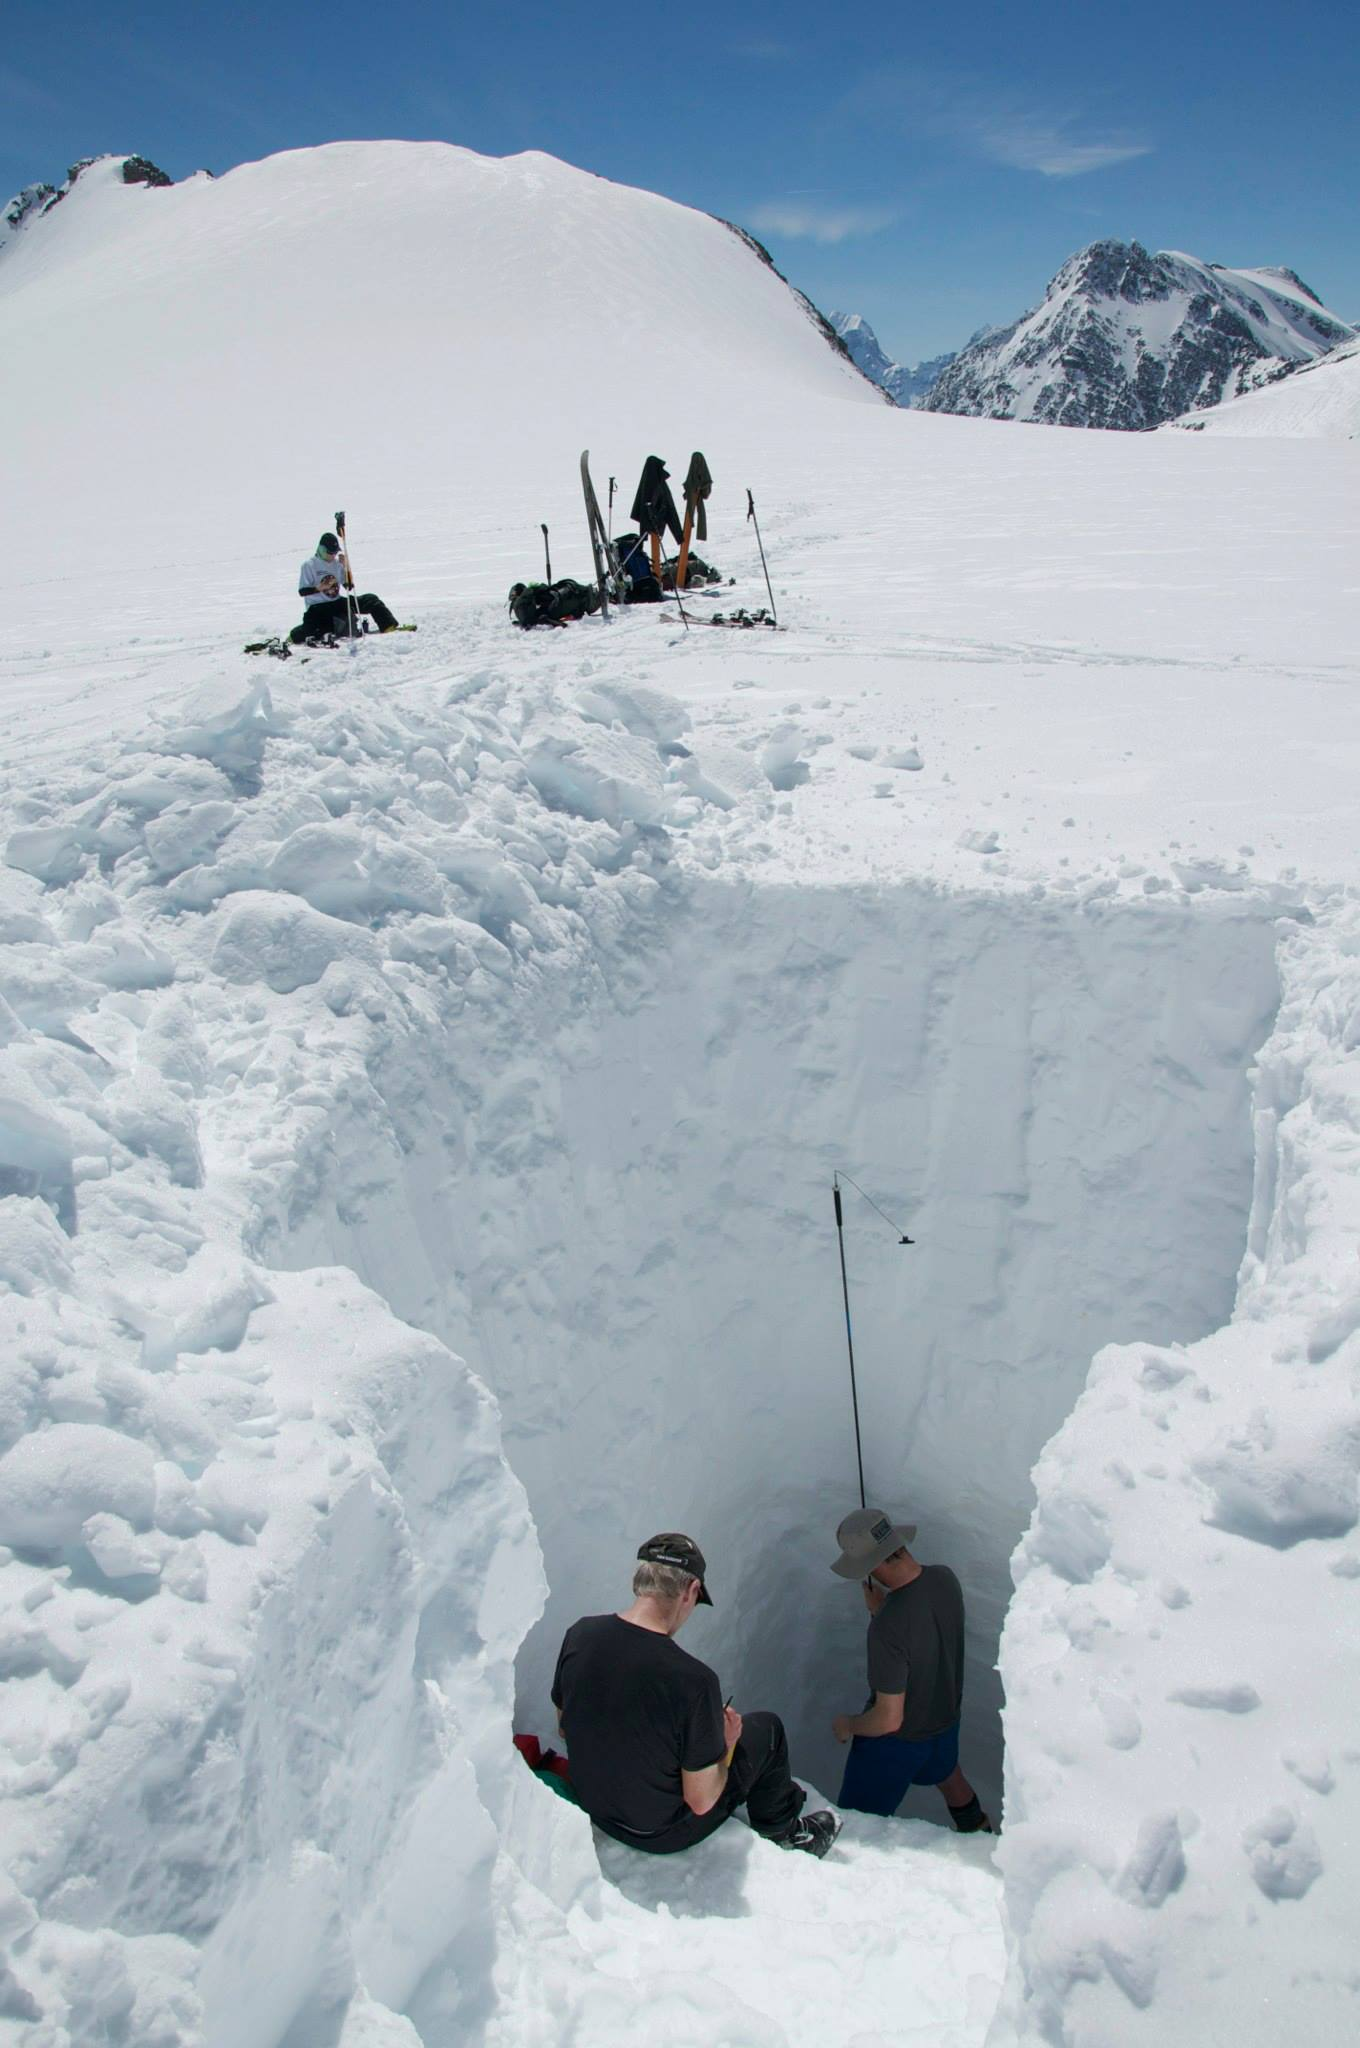
\includegraphics[width=0.4\textwidth]{snowpit.jpg}
  \caption{Measuring snow depth and density in a snow pit located in the accumulation area of Haig Glacier, Rocky Mountains}
        \label{snowpit}
\end{figure}

The most direct way of measuring snow depth is by probing. To determine the snowpack thickness, the height of the snow above the surface at the end of the previous melt season is measured. Usually, a number of snow height measurements are obtained close to each other and the mean value is taken to be representative of that location. For example, \cite{Machguth2006} took the mean of nine snow probe measurements within a 7 m radius as representative of a single measurement location.  

In the ablation zone of a glacier snow depth is easy to measure because the interface between the end-of-summer melt surface and the winter accumulation is well defined (i.e. glacier ice) \citep{McGrath2015}. In the accumulation zone however, the snow surface at the end of the melt season may not be easily distinguishable from the winter accumulation \citep{Grunewald2010}. It is common for the accumulation zone to have a heterogeneous surface at the end of the melt season; some areas do not experience any melt, while other areas experience some melt and the melt water percolates through the snow and firn. Melt water generated from warm weather or rain events, especially in the early and late parts of the accumulation season, can refreeze in the snowpack to form ice lenses \citep{Sold2014}. As a result, the desired interface can be difficult to detect and probing in the accumulation zone can result in erroneous depth measurements. If a probe penetrates into the dense snow or firn, the snowpack will seem deeper and if the probe hits an ice lens, the snow pack will seem shallower \citep{Sold2013}. Snow pits and cores are therefore used to examine snow and firn layers and to determine where the current season's snow begins.

To determine the basin-wide snow distribution, point snow depth measurements from probing need to be interpolated and extrapolated. This is often done using a statistical regression on parameters such as slope, aspect, curvature and susceptibility to wind redistribution \citep[e.g.][]{Wheler2014,McGrath2015}. A regression generates an equation that is site specific and is used to estimate accumulation for each gridcell based on the gridcell values of topographic parameters. 

Snow probing is the simplest and oldest method used to determine accumulation. At the most basic level, it requires little more than a probe to determine depth, a way to determine location (such as a hand-held GPS) and a shovel to dig snow pits (see Figure \ref{snowpit}). Furthermore, this method directly measures snow depth so no data processing or corrections are needed. Depth uncertainty is simple to quantify and is often taken to be the standard deviation of measurements that are taken close together \citep{Sold2013}. 

There are however many drawbacks to this method. \textit{In situ} probing and digging snow pits is time-consuming \citep{Deems2006}, limiting the number of measurements that can be made. As a result, accumulation variability is under-represented and spatial variability in accumulation is difficult to capture \citep{Sold2014}. Measurement is also limited to areas that are both accessible and safe for researchers. In complex terrain many areas cannot be surveyed, resulting in data gaps. \cite{Sold2013} noted that this systematic bias can result in incorrect values of glacier-wide accumulation, particularly because inaccessible areas such as cliffs and ridges have relatively low accumulation (due to wind erosion) and heavily crevassed areas can accumulate deep snow packs. 

\subsection{Sampling Design}

Optimal sampling schemes for snow probing are central to accurately estimating snow distribution and mass balance from \textit{in situ} measurements. Measuring snow depth and travelling between measurement locations is both time consuming and can disturb the snow so care must be taken to choose a sampling scheme that avoids bias, allows for the greatest variability to be measured and minimizes distance travelled \citep{Shea2010}. A design that maximizes accuracy and minimizes effort is therefore desired \citep{Elder1991} and both theoretical \citep{Trujillo2015} and applied \citep{Kronholm2004,Shea2010} investigations of various sampling designs have been pursued. There are a number of different designs that have been employed to obtain point measurements, including pure random, linear random, nested, gridded random and gridded. 

A purely random distribution of points (Figure \ref{schemes}(a)) is favourable because it avoids all bias, results in the most accurate representation of the true spatial patterns and is likely to capture the most variability \citep{Kronholm2007, Shea2010}. Logistically, it is difficult to successfully measure all points in the study area because some may be impossible to access and some may be disrupted during travel or measurement. A purely random design often results in inefficient travelling routes, thus decreasing the number of possible point measurements. \cite{Elder1991} show a simple basin-wide random sample is a less optimal sampling scheme than a stratified random sample that accounts for known variation. 

Linear-random sampling schemes impose a structure to traverse as much of the study area as possible but allow for a random distance between sampling points. An example of this scheme is the `star', created by \cite{Shea2010}. A significant advantage of this scheme is that it was designed to minimize distance travelled while still measuring snow properties in various orientations and various distances apart, which reduces bias. However, since the observer travels in straight transects there is still a potential to miss smaller features or ones that parallel the transects (spatial autocorrelation). \cite{Shea2010} used comparative Monte Carlo simulations to validate that the star scheme performs as well as or better than other (more structured) sampling methods and that it converges to the true distribution as well as a purely random scheme. One example of a linear-random sampling scheme can be seen in Figure \ref{schemes}(b). Linear-random sampling can also be done in an `hourglass' shape with an inscribed circle (referred to as an hourglass sampling scheme). As seen in Figure \ref{schemes}(f), this pattern allows sampling in all directions and captures a wide range of snow depths from the underlying snow distribution (Parr, C., 2016 personal communication).

\begin{figure}[H]
\begin{minipage}[c][11cm][t]{.33\textwidth}
        \vspace*{\fill}
  \centering
  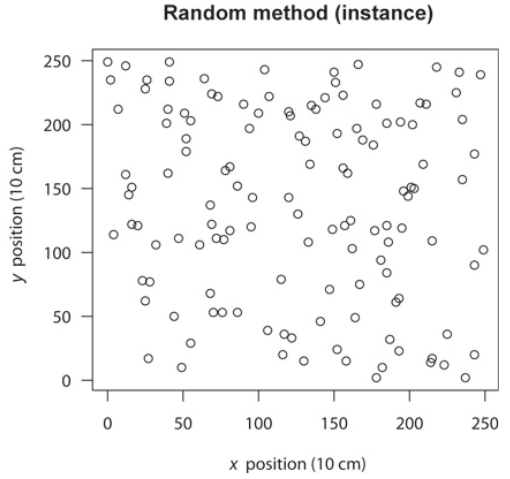
\includegraphics[width=5cm,height=4.5cm]{random.png}
  \subcaption{Pure random}
  \par\vfill
  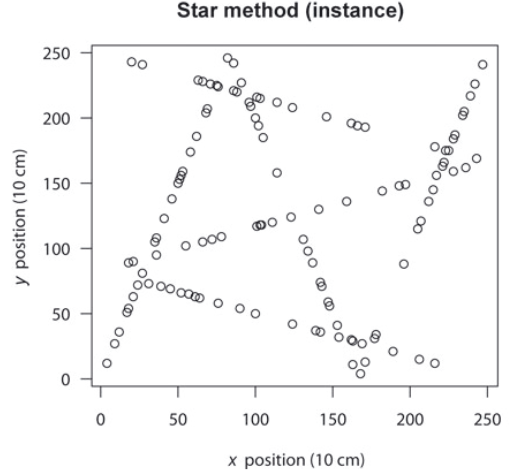
\includegraphics[width=5cm,height=4.5cm]{star.png}
  \subcaption{Star}
\end{minipage}%
\begin{minipage}[c][11cm][t]{.33\textwidth}
        \vspace*{\fill}
  \centering
  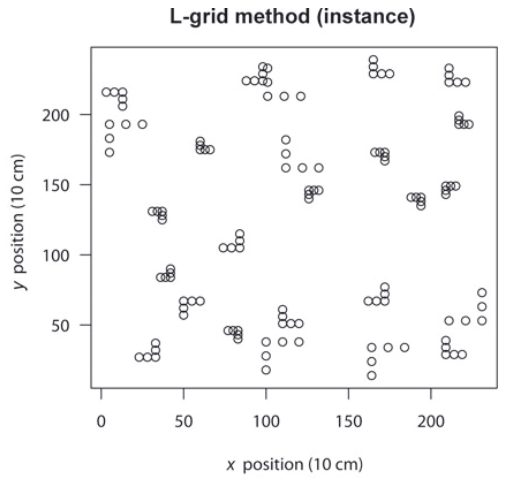
\includegraphics[width=5cm,height=4.5cm]{Lgrid.png}
  \subcaption{L-grid}
\par\vfill
  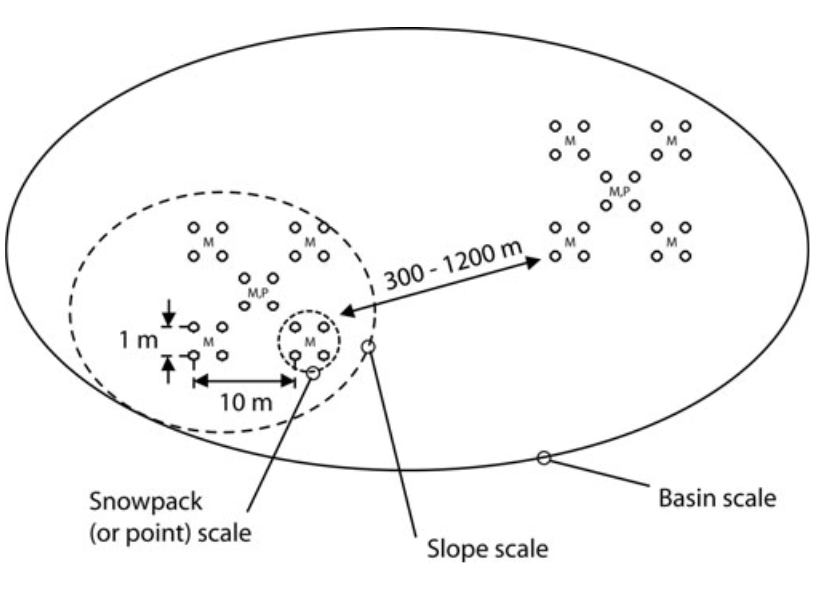
\includegraphics[width=5cm,height=4.5cm]{nested.png}
  \subcaption{Nested}
\end{minipage}%
\begin{minipage}[c][11cm][t]{.33\textwidth}
        \vspace*{\fill}
  \centering
    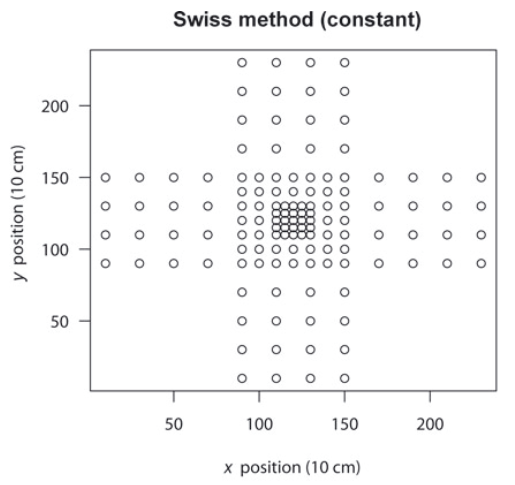
\includegraphics[width=5cm,height=4.5cm]{swiss.png}
  \subcaption{Swiss grid}
   \par\vfill
   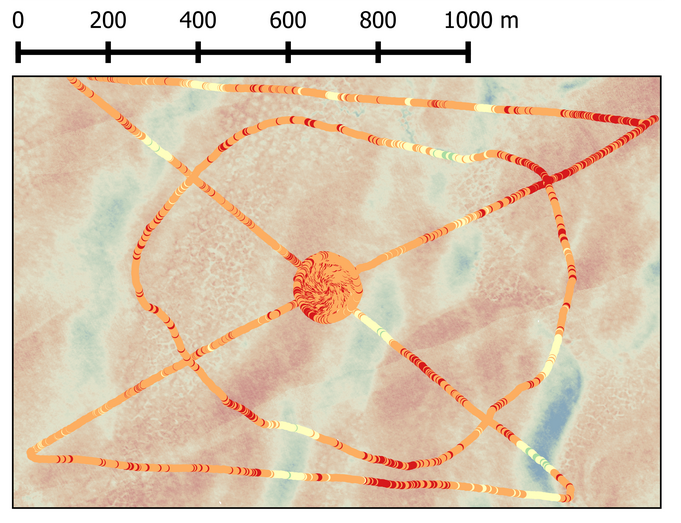
\includegraphics[width=5cm,height=4.5cm]{hourglass.png}
  \subcaption{Hourglass}
\end{minipage}
\caption{Examples of snow sampling schemes. Figures (a), (b), (c) and (e) from \cite{Shea2010}. Figure (d) from \cite{Schweizer2008}. Figure (f) from Parr, C., (2016 personal communication).}
\label{schemes}
\end{figure}

Gridded-random designs (Figure \ref{schemes}(c)) involve dividing the study area into equal sized areas and then sampling randomly within each area. The L-grid is an example of this scheme \citep{Bellaire2008, Elder2009, Bellaire2011}. In this scheme, the study area is divided into a grid and in each cell a random location is chosen as the start of the transect. The cardinal direction and measurement spacing of the transect are chosen randomly. Transects consist of five measurements, with three in the first direction selected and two perpendicular to this, forming an `L' shape. This scheme has a small error bias (maintains randomness), while allowing for more efficient measurement \citep{Shea2010}. Compared to the star scheme, the L-grid does not have a consistent travel distance and involves constant reorientation and finding of transect start locations, which decreases its efficiency. 

Nested sampling (Figure \ref{schemes}(d)) is a scheme that maintains a certain sampling pattern and applies it at various length scales. For example, \cite{Schweizer2008} took four point measurements in a 1\,m square and did this 10\,m apart to form another square. The set of measurements was then repeated 300--1200\,m away to capture variability at the basin scale. Hierarchal trees are often used to determine nested sampling locations. For example, \cite{Watson2006} and \cite{Kasurak2011} use hierarchal sampling to divide the study area into regions (often discontinuous) that are likely to have a similar snow distribution and low variance, which means they require fewer sampling locations. Nested sampling requires that the observer predetermine parameters that affect the spatial pattern of the variable. Often, remote sensing is used to obtain these parameters so the resolution of regions is limited to that of the remote sensing images (typically 30\,m resolution). The variability that exists at scales less than the grid-size of the images is classified as being caused by `random' effects, which are assumed to be unbiased and unpredictable \citep{Watson2006}. Nested sampling is well suited for regions with many complex and interacting parameters. For example, \cite{Watson2006} used a hierarchal tree with time (traveling between locations), elevation, vegetation and solar radiation at various length scales to create subgroup to sample. 

Gridded sampling designs (Figure \ref{schemes}(e)) use regular measurement intervals in a grid pattern. Many variations of this scheme exist \citep{Molotch2005a, Kronholm2007, Lopez2011} with the most popular one being the Swiss cross \citep{Kronholm2004}. This nested arrangement allows for a larger area to be covered than a fully quadratic grid and measures at various spatial scales, leading to more reliable geospatial statistics. However, measurements are biased by regularly spaced intervals and linear orientation, which could result in an under representation of the snow distribution further from the centre. 

\section{Snow distribution on glaciers}
While studies of snow distribution in alpine regions are plentiful \citep[and sources within]{Clark2011} there are comparatively few studies on the distribution of snow on glaciers. Although glaciers are often found in alpine environments, they present a different setting for accumulation. The freezing temperatures of glacier ice allow for snow to stick earlier than on the surrounding rocks, which can be above freezing especially in the early part of the accumulation season. Additionally, the surface of a glacier is often less steep than the surrounding peaks, which allows for snow to deposit more easily. The margin of the glacier can also accumulate snow from avalanches released from the surrounding terrain \citep{Bloschl1991, Mott2008}. Further, most glaciers do not support vegetation, which has significant effects on snow accumulation in many alpine basins \citep{Pomeroy1999}. \cite{Alford1985} found that in open alpine areas with snow fields and small cirque glaciers there was a wide range of SWE values over a relatively small range of elevation, while in the montane areas there was a strong relationship between elevation and SWE, where SWE values increased rapidly with elevation. Since few studies have been done on this topic, it is difficult to say whether snow distribution on glaciers is fundamentally different than that of an alpine basin. This lack of snow variability quantification points to a significant gap in the literature.

\cite{Winther1998} conducted one of the first accumulation variability studies on a glacier. A GPR system was used to measure snow depth along three large transects on Spitsbergen, Svalbard. It was found that the accumulation--elevation gradients varied considerably and that regional variability was large, with almost 50$\%$ more accumulation on the eastern coast and a minimum in accumulation in the inland locations. A number of subsequent accumulation studies in Svalbard have since been conducted. \cite{Palli2002} used GPR along longitudinal profiles of Nordenskj\"{o}ldbreen and found 40 -- 60$\%$ spatial variability over short distances. \cite{Grabiec2011} compared snow distribution on four types of glaciers in Svalbard. It was observed that the land-terminating mountain glacier had a simple altitudinal gradient while the outlet glacier had a much weaker correlation and more wind-redistributed snow. The orientation and shape of the glacier also had a significant impact on snow accumulation, with the glaciers that were oriented parallel to the dominant wind direction having stronger altitudinal gradients. Another glacier that was observed had no altitudinal gradient, so snow distribution was determined by complex local conditions. The ice cap that \cite{Grabiec2011} studied had all of these types of distributions in different areas.

\cite{Machguth2006} conducted an airborne GRP survey of two adjacent glaciers in Switzerland. The lower part of the larger valley glacier showed a clear correlation between altitude and snow accumulation. The upper part of the glacier and the adjacent smaller glacier had no altitudinal trend and the fluctuations in depth were large. Additionally, the accumulation was 40$\%$ lower on the smaller glacier. The altitudinal trend is a well documented pattern and was thought to be a result of melt that occurred during warmer weather, which is more pronounced at lower elevations. Spatial variability of precipitation and redistribution of snow are believed to have resulted in the high spatial variability in higher parts of the study area. Since the majority of the precipitation events originated from one direction and the large glacier was on the lee side of a ridge, it experienced preferential deposition. Meanwhile, the smaller glacier was further along the storm track so it received less precipitation. Overall, \cite{Machguth2006} showed that snow distribution on glaciers is not simply a function of altitude, which corroborated research done in other alpine catchments.

The most recent and comprehensive study of snow distribution on glaciers was done by \cite{McGrath2015}. This study focused on seven Alaskan glaciers of various sizes, orientations and distances from the Pacific Ocean. \cite{McGrath2015} found that SWE was highly variable (40$\%$ differences) at the hillslope-scale and was especially large in the ablation area (which has a rough surface due to the presence of crevasses). The dominant control on SWE distribution was elevation, but multiple terrain parameters were needed to capture most of the variance; after elevation, wind exposure explained the most variance. \cite{McGrath2015} also found that four of the study glaciers exhibited a rapid increase in SWE variability between measurements separated by $\sim$150 m and a slow increase in variability beyond. The three other study glaciers exhibited a gradual increase in variability within increasing distance between measurements over the entire range. Although this was not a detailed investigation of observed length scales, it highlights spatial heterogeneity of snow distribution on glaciers.

The study done by \cite{Walmsley2015} contains the longest record of spatial distribution of snow accumulation. \cite{Walmsley2015} analyzed 48 and 44 year records of two Norwegian glaciers for inter-annual stability in distribution patterns. It was found that snow accumulation is spatially heterogeneous yet it exhibits robust time stability in distributions. Reliability maps were then used to reduce the sampling scheme to one index site as well as a transect with 50 m elevation intervals for each glacier. Although winter balance reconstructions produced values within 0.15 m water equivalent, it was determined that a centreline transect underestimated winter balance. Transverse transects were therefore recommend as an addition to the sampling scheme to improve reliability.

The majority of studies that have examined snow distribution on glaciers have been done with either airborne or ground-based radar \citep[e.g.][]{Winther1998,Machguth2006, Grabiec2011, Pelt2014,McGrath2015}. In general, the radargrams provided valuable information but ground truthing by probing was always conducted. \cite{Gusmeroli2014} also did a small GPR survey on an Alaskan glacier and found that GPR reflections were difficult to identify in areas of the glacier that had high debris content on the surface or in the upper part of the accumulation area. \cite{Sold2013} did an extensive study that compared snow distribution values obtained by using probing, GPR and DEM subtraction with lidar. All three methods showed an overall elevation trend but with significant small-scale variability (for a comparison of the three methods and their relative benefits, see Section \ref{sec:comparemethods}). \cite{Pelt2014} used GPR and a surface-energy balance model coupled with a snow model to examine accumulation variability. It was found that terrain parameters such as slope and curvature were good indicators of preferential deposition. Additionally, \cite{Pelt2014} calculated that small-scale variability of snow accumulation had a negligible effect on the mean net mass balance in the accumulation zone and a negative impact of $-$0.09 \,m\,w.e. a$^{-1}$ in the ablation area.

\cite{Dadic2010} examined snow distribution on glaciers using a dynamic model. This study specifically looked at the effect of wind on snow accumulation and found that glacierized areas with the largest accumulation also experienced the lowest horizontal wind speeds and highest downward wind velocity. Preferential deposition was highest (positive or negative) in troughs located close to steep slopes, where updrafts and down drafts led to decreased and enhanced deposition, respectively. In general, the wind speed was controlled by small-scale topography and had a significant impact on accumulation. 

Although there are still relatively few studies of snow distribution on glaciers, the work described above provides a good starting point for such investigations. Comparisons of variability between neighbouring glaciers and within a basin are both important areas of research.

\section{Research scope}
\label{sec:ResearchScope}
The overarching goal of this thesis is to address the need for a multi-scale investigation of snow distribution on alpine glaciers in the St. Elias Mountains. I focus on estimating winter surface mass balance (`winter balance'), which is the net accumulation and ablation of snow over the winter season \citep{Cogley2011}, at multiple scales on three alpine glaciers in the Donjek Range (Table \ref{tab:glacierstats}). The objectives of this study are to (1) critically examine methods of converting direct snow depth and density measurements to distributed estimates of winter balance and (2) identify sources of uncertainty, evaluate their magnitude and assess their combined contribution to uncertainty in glacier-wide winter balance. 

\begin{sidewaystable}[]
\centering
\caption{Physical characteristics of the study glaciers and May 2016 winter-balance survey details, including number of snow-depth measurement locations along transects ($n_{\mathrm{T}}$), total length of transects ($d_{\mathrm{T}}$), number of combined snow pit and Federal Sampler density measurement locations ($n_{\rho}$) and number of zigzag surveys ($n_{\mathrm{zz}}$).}
\label{tab:glacierstats}
\begin{tabular}{cccccccccccc}
\midrule
\textbf{} & \textbf{Location} & \multicolumn{3}{c}{\textbf{Elevation (m a.s.l)}} & \textbf{Slope ($^{\circ}$)} & \multirow{2}{*}{\textbf{\begin{tabular}[c]{@{}c@{}}Area \\ (km$^2$)\end{tabular}}} & \multirow{2}{*}{\textbf{\begin{tabular}[c]{@{}c@{}}Survey\\ Dates\end{tabular}}} & \multicolumn{4}{c}{\textbf{Survey Details}} \\
 & UTM Zone 7 & \textit{Mean} & \textit{Range} & \textit{ELA} & \textit{Mean} &  &  & $n_{\mathrm{T}}$ & $d_{\mathrm{T}}$ (km) & $n_{\rho}$ & $n_{\mathrm{zz}}$ \\ \midrule
\textbf{Glacier 4} & \begin{tabular}[c]{@{}c@{}}595470 E\\ 6740730 N\end{tabular} & 2344 & 1958--2809 & $\sim$2500 & 12.8 & 3.8 & 4--7 May 2016 & 649 & 13.1 & 10 & 3 \\
\textbf{Glacier 2} & \begin{tabular}[c]{@{}c@{}}601160 E\\ 6753785 N\end{tabular} & 2495 & 1899--3103 & $\sim$2500 & 13.0 & 7.0 & 8--11 May 2016 & 762 & 13.6 & 11 & 3 \\
\textbf{Glacier 13} & \begin{tabular}[c]{@{}c@{}}604602 E\\ 6763400 N\end{tabular} & 2428 & 1923--3067 & $\sim$2380 & 13.4 & 12.6 & 12--15 May 2016 & 941 & 18.1 & 20 & 4
\end{tabular}
\end{sidewaystable}

\subsection{Study site}

The St. Elias Mountains (Fig. \ref{fig:Sampling}a) rise sharply from the Pacific Ocean, creating a significant climatic gradient between coastal maritime conditions, generated by Aleutian--Gulf of Alaska low-pressure systems, and interior continental conditions, driven by the Yukon--Mackenzie high-pressure system \citep{Taylor1969}. The boundary between the two climatic zones is generally aligned with the divide between the Hubbard and Kaskawulsh Glaciers, approximately 130\,km from the coast. Research on snow distribution and glacier mass balance in this area is limited. A series of research programs, including Project ``Snow Cornice''  and the Icefield Ranges Research Project, were operational in the 1950s and 60s \citep{Wood1948, Danby2003} and in the last 30 years, there have been a few long-term studies on selected alpine glaciers \citep[e.g.][]{Clarke2014} as well as several regional studies of glacier mass balance and dynamics \citep[e.g.][]{Arendt2008, Burgess2013,Waechter2015}.

We carried out winter balance surveys on three unnamed glaciers in the Donjek Range of the St. Elias Mountains. The Donjek Range is located approximately 40 km to the east of the regional mountain divide and has an area of about $30\times30$\,km$^2$. Glacier 4, Glacier 2 and Glacier 13 (labelling adopted from \cite{Crompton2016}) are located along a southwest-northeast transect through the range (Fig. \ref{fig:Sampling}b, Table \ref{tab:glacierstats}). These small alpine glaciers are generally oriented southeast-northwest, with Glacier 4 having a predominantly southeast aspect and Glaciers 2 and 13 have generally northwest aspects. The glaciers are situated in valleys with steep walls and have simple geometries. Based on a detailed study of Glacier 2  \citep{Wilson2013} and related theoretical modelling \citep{Wilson2013a} we suspect all of the study glaciers to be polythermal. 

\begin{figure}
	\centering
	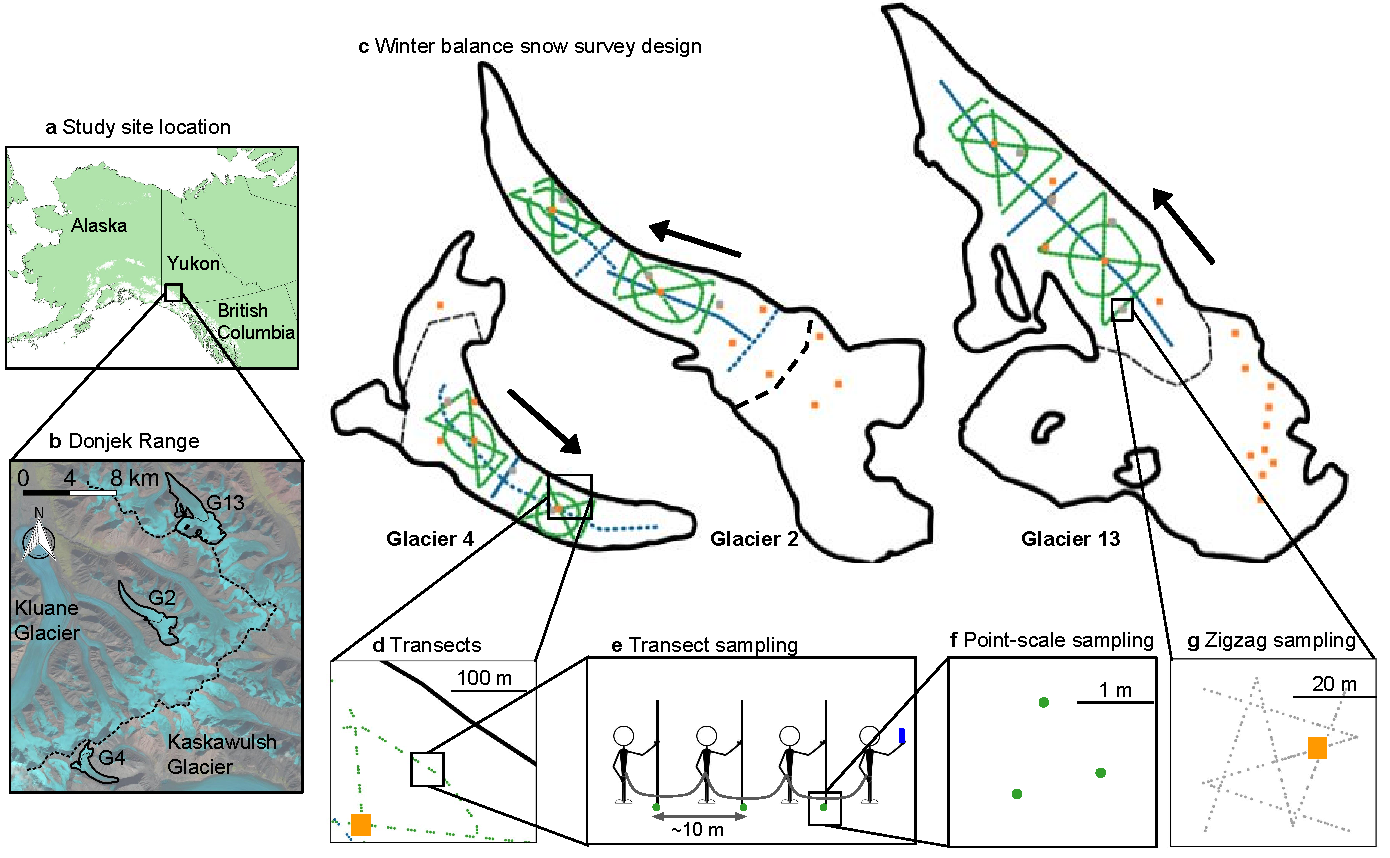
\includegraphics[width =0.9\textwidth]{Sampling.pdf}\\
	\caption{Study area location and sampling design for Glaciers 4, 2 and 13. (a) Study region in the Donjek Range of the St. Elias Mountains of Yukon, Canada. (b) Study glaciers located along a southwest-northeast transect through the Donjek Range. The local topographic divide is shown as a dashed line. Imagery from Landsat8 (5 September 2013, data available from the U.S. Geological Survey). (c) Details of the snow-survey sampling design, with centreline and transverse transects (blue dots), hourglass and circle designs (green dots) and locations of snow density measurements (orange squares). Arrows indicate ice-flow directions. Approximate location of ELA on each glacier is shown as a black dashed line. (d) Close up of linear and curvilinear transects. (e) Configuration of navigator and observers. (f) Point-scale snow-depth sampling. (g) Linear-random snow-depth measurements in `zigzag' design (grey dots) with one density measurement (orange square) per zigzag.}
	\label{fig:Sampling}
\end{figure}


 \begin{figure}
           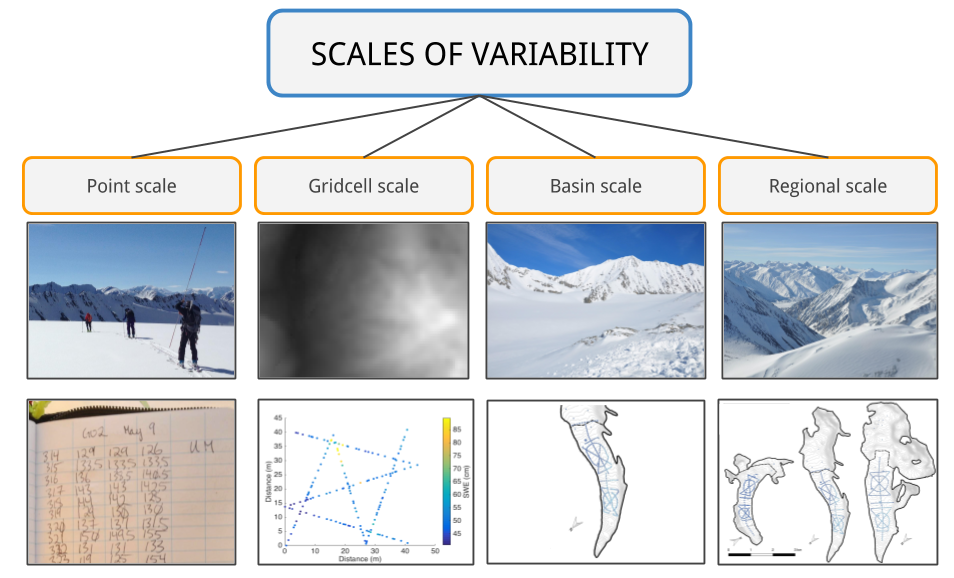
\includegraphics[width = 0.95\textwidth]{ScalesOfVariability.png}
       \caption{Visualization of the four spatial scales investigated. The lower panels show examples of the data analyzed at each scale.}
       \label{fig:flowchart_scales}
\end{figure}

\subsection{Overview of research}

Commonly applied, low-complexity methods of measuring and estimating winter balance are used in the interest of making the results broadly applicable. An extensive snow survey is conducted, using a combination of snow-depth probing and two snow density measurement techniques, on three alpine glaciers in the Donjek Range. A combination of statistical techniques is then used to investigate spatial variability at multiple scales. Throughout this thesis, four spatial scales that are relevant to estimating winter balance are discussed: point, gridcell, basin (or glacier-wide) and regional (Figure \ref{fig:flowchart_scales}). 

The thesis work is centred around the process of converting point-scale, direct measurements of snow depth and density to estimates of glacier-wide winter balance using statistical models. The project is structured in four main components (Figure \ref{fig:flowchart_project}). First, observations are described using basic statistics and a variety of density assignment methods are investigated. Second, regression and kriging methods are used to interpolate winter balance data. An evaluation of the various interpolation techniques is then done and significant topographic parameters are identified. Third, a Monte Carlo approach is used to quantify the effect of several sources of uncertainty on the glacier-wide winter-balance uncertainty. Fourth, the transferability of statistical relationships between glaciers is examined and an winter-balance gradient on the continental side of the St. Elias Mountains is identified.

\subsection{Thesis structure}
The thesis is structured to follow the visual representation of the research project presented in Figure \ref{fig:flowchart_project}. Chapter 2 provides a detailed description of the intended and executed field measurements as well as a description of data processing methods. Chapter 3 focuses on presenting snow depth and density measurements as well as subsequent data processing. This chapter details various methods of assigning density values to unmeasured locations, converting snow depth and density to winter balance, as well as calculating topographic parameters used for interpolation. Chapter 4 details three interpolation methods used to obtain distributed estimates of winter balance. Linear regression, simple kriging and regression kriging are compared and insights gained through the interpolation processes about controls on winter balance are discussed. Chapter 5 examines estimates of winter balance and how grid-scale variability, density assignment and data interpolation interact to create uncertainty in estimates of winter balance. Chapter 6 examines winter balance at the regional-scale. The transferability of linear regression models between glaciers is investigated and glacier-wide winter balances are related to the regional winter-balance gradient along the continental side of the St. Elias Mountains. 

 \begin{figure}[H]
 \centering
           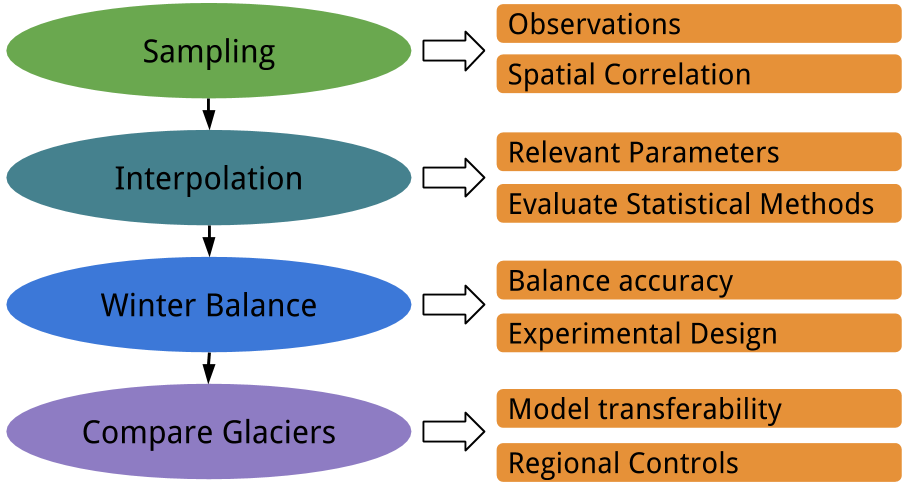
\includegraphics[width =0.7\textwidth]{MastersFlow.png}
       \caption{Visual representation of research project. General scope is described on the left (ovals) and specific investigations are shown on the right (squares).}
       \label{fig:flowchart_project}
\end{figure}

\section{Summary}
Snow accumulation plays a central role in alpine hydrology and has a prominent impact on glacier mass balance. In mountainous regions, accumulation is highly variable on point, hillslope, watershed and regional scales. The contribution of accumulation to glacier mass balance is controlled mainly by the distribution of snow. Processes such as orographic lifting, preferential deposition and wind redistribution, all arising from the interaction of atmospheric conditions and topography, strongly affect snow distribution. Statistical models have been used to relate meteorological and topographic variables to snow accumulation in order to better understand the effects of these processes. These models rely on accurate measurement of snow distribution, which can be achieved by determining snow water equivalent values from snow density and depth. Results from previous studies of accumulation on glaciers have shown considerable spatial variability at many scales resulting from interactions between topography and atmospheric conditions. 

Accumulation in the St. Elias Mountains is poorly understood. There is a need to quantify winter balance in this region and how it varies both between glaciers and within glacierized basins. The study described in this thesis is the first within the St. Elias Mountains to examine winter balance variability at the point, gridcell, basin and regional scales. Well-established methods are applied to estimate winter balance at multiple scales. The data are used to investigate the role of topography in determining snow distribution, uncertainty in estimating glacier-wide winter balance, the transferability of statistical relationships and regional differences in distributed winter balance. 


%%%%%%%%%%%%%%%%%%%%%%%%%%%%%%%%%%%
% Field methods and data processing
%%%%%%%%%%%%%%%%%%%%%%%%%%%%%%%%%%%

\chapter{Field methods and data processing}

The thesis work is centred around data collected during a snow survey, which occurred during a two week period in May 2016 on three glaciers within the Donjek Range, St. Elias Mountains, Yukon, Canada. The intent of the survey design was to capture the spatial variability of winter balance (WB) at various scales. Measurement locations are concentrated in the ablation areas of the glaciers, where a clearly defined boundary between snow and ice allows for accurate identification of snow that has accumulated during the previous winter season. Snow depth was measured using avalanche probes, and snow density was measured using a wedge sampler in snow pits and using a Federal Sampler. We intended to use a firn corer to measure winter balance in the accumulation area, but cold snow combined with positive air temperatures led to cores being unrecoverable. Snow depth and density data were manually recorded in the field, and waypoints, from which measurement locations were later estimated, were recorded using a single-band GPS. 

The following sections describe the design of the snow survey, how the survey was implemented in the field and how the data were digitized. Initial processing methods to obtain data for future analysis are also detailed. Section 2.1 describes the survey naming scheme and shows planned snow measurement locations. Section 2.2 provides details of the snow survey and use of various snow measurement tools. Section 2.3 describes how the data are processed to obtain the point- and gridcell-scale WB data that are used for analysis in subsequent sections. Appendix \ref{app:GPSwaypoints} describes the steps needed to create GPS waypoints and Appendix \ref{app:fieldmaps} contains maps that were created for fieldwork.

%%%%
\section{Experimental design}
%%%%
\label{sec:FieldDesign}

\subsection{Sampling scheme and naming system}

Three glaciers within the Donjek Range were chosen as study sites (Figure \ref{studysites}). Glaciers in the Donjek Range are unnamed, but working names have been employed by \cite{Crompton2016} and are adopted for this work. Glacier 4, Glacier 2 and Glacier 13 were selected. These glaciers were chosen because they are distributed throughout the Donjek Range and are located increasingly further from the large-scale topographic divide (located at the head of the Kaskawulsh Glacier \citep{Taylor1969}). The three glaciers are also located on different sides of the range-scale topographic divides, which run roughly from west to east in the southern area and from south to north in the eastern area and form an `L' shape. Glacier 4 is located on the southern side of the west-east arm, Glacier 2 is located on the northern side of the west-east arm and the western side of the north-south arm and Glacier 13 is located on the eastern side of the north-south arm. These small alpine glaciers are generally oriented southeast-northwest, with Glacier 4 having a predominantly southeast aspect and Glaciers 2 and 13 have generally northwest aspects. The glaciers are situated in valleys with steep walls and have simple geometries. Within the Donjek Range, these glaciers have good coverage in the SPIRIT SPOT-5 DEM, which provides the highest resolution gridded topographic data available for this area. Additionally, most of the area of the three glaciers is accessible on foot and the total area is small enough (see Table \ref{tab:glacierstats}) to allow for reasonable coverage using point measurements.

The sampling scheme for each glacier was chosen to facilitate comparison between glaciers. Each glacier was divided into the accumulation area, upper ablation area and lower ablation area. In the accumulation area, a central snow pit location was chosen. Approximately ten snow coring locations were chosen throughout the accumulation area. Steep sections and glacier margins were avoided. In both the upper and lower ablation area a number of linear and curvilinear transects were planned and included an `hourglass and circle' (Parr, C., 2016 personal communication) as well as transverse and midline transects. The length and width of each transect was adjusted to span the full width of the glacier. Snow pit locations in the ablation area were chosen to be at the centre of each hourglass. An overview of the sampling design can be seen in Figure \ref{transect_planned}.

The full ablation area was also divided into seven zones of approximately equal elevation intervals. Three locations within each zone were then randomly selected (using QGIS) for zigzag \citep{Shea2010} measurements (Figure \ref{zigzag_planned}) and the three locations were randomly prioritized. The goal was to complete one zigzag survey in each zone. If possible, the measurement would be completed at the `Priority A' location but if it was not possible due to dangerous conditions then the `Priority B' or `Priority C' locations would be chosen. This allowed for random locations to be used but with the flexibility to adjust locations in the field. Federal Sampler measurements (described below) would be taken within each zigzag and at snow pit locations within the ablation area.  

\begin{figure}
	\centering
	\fbox{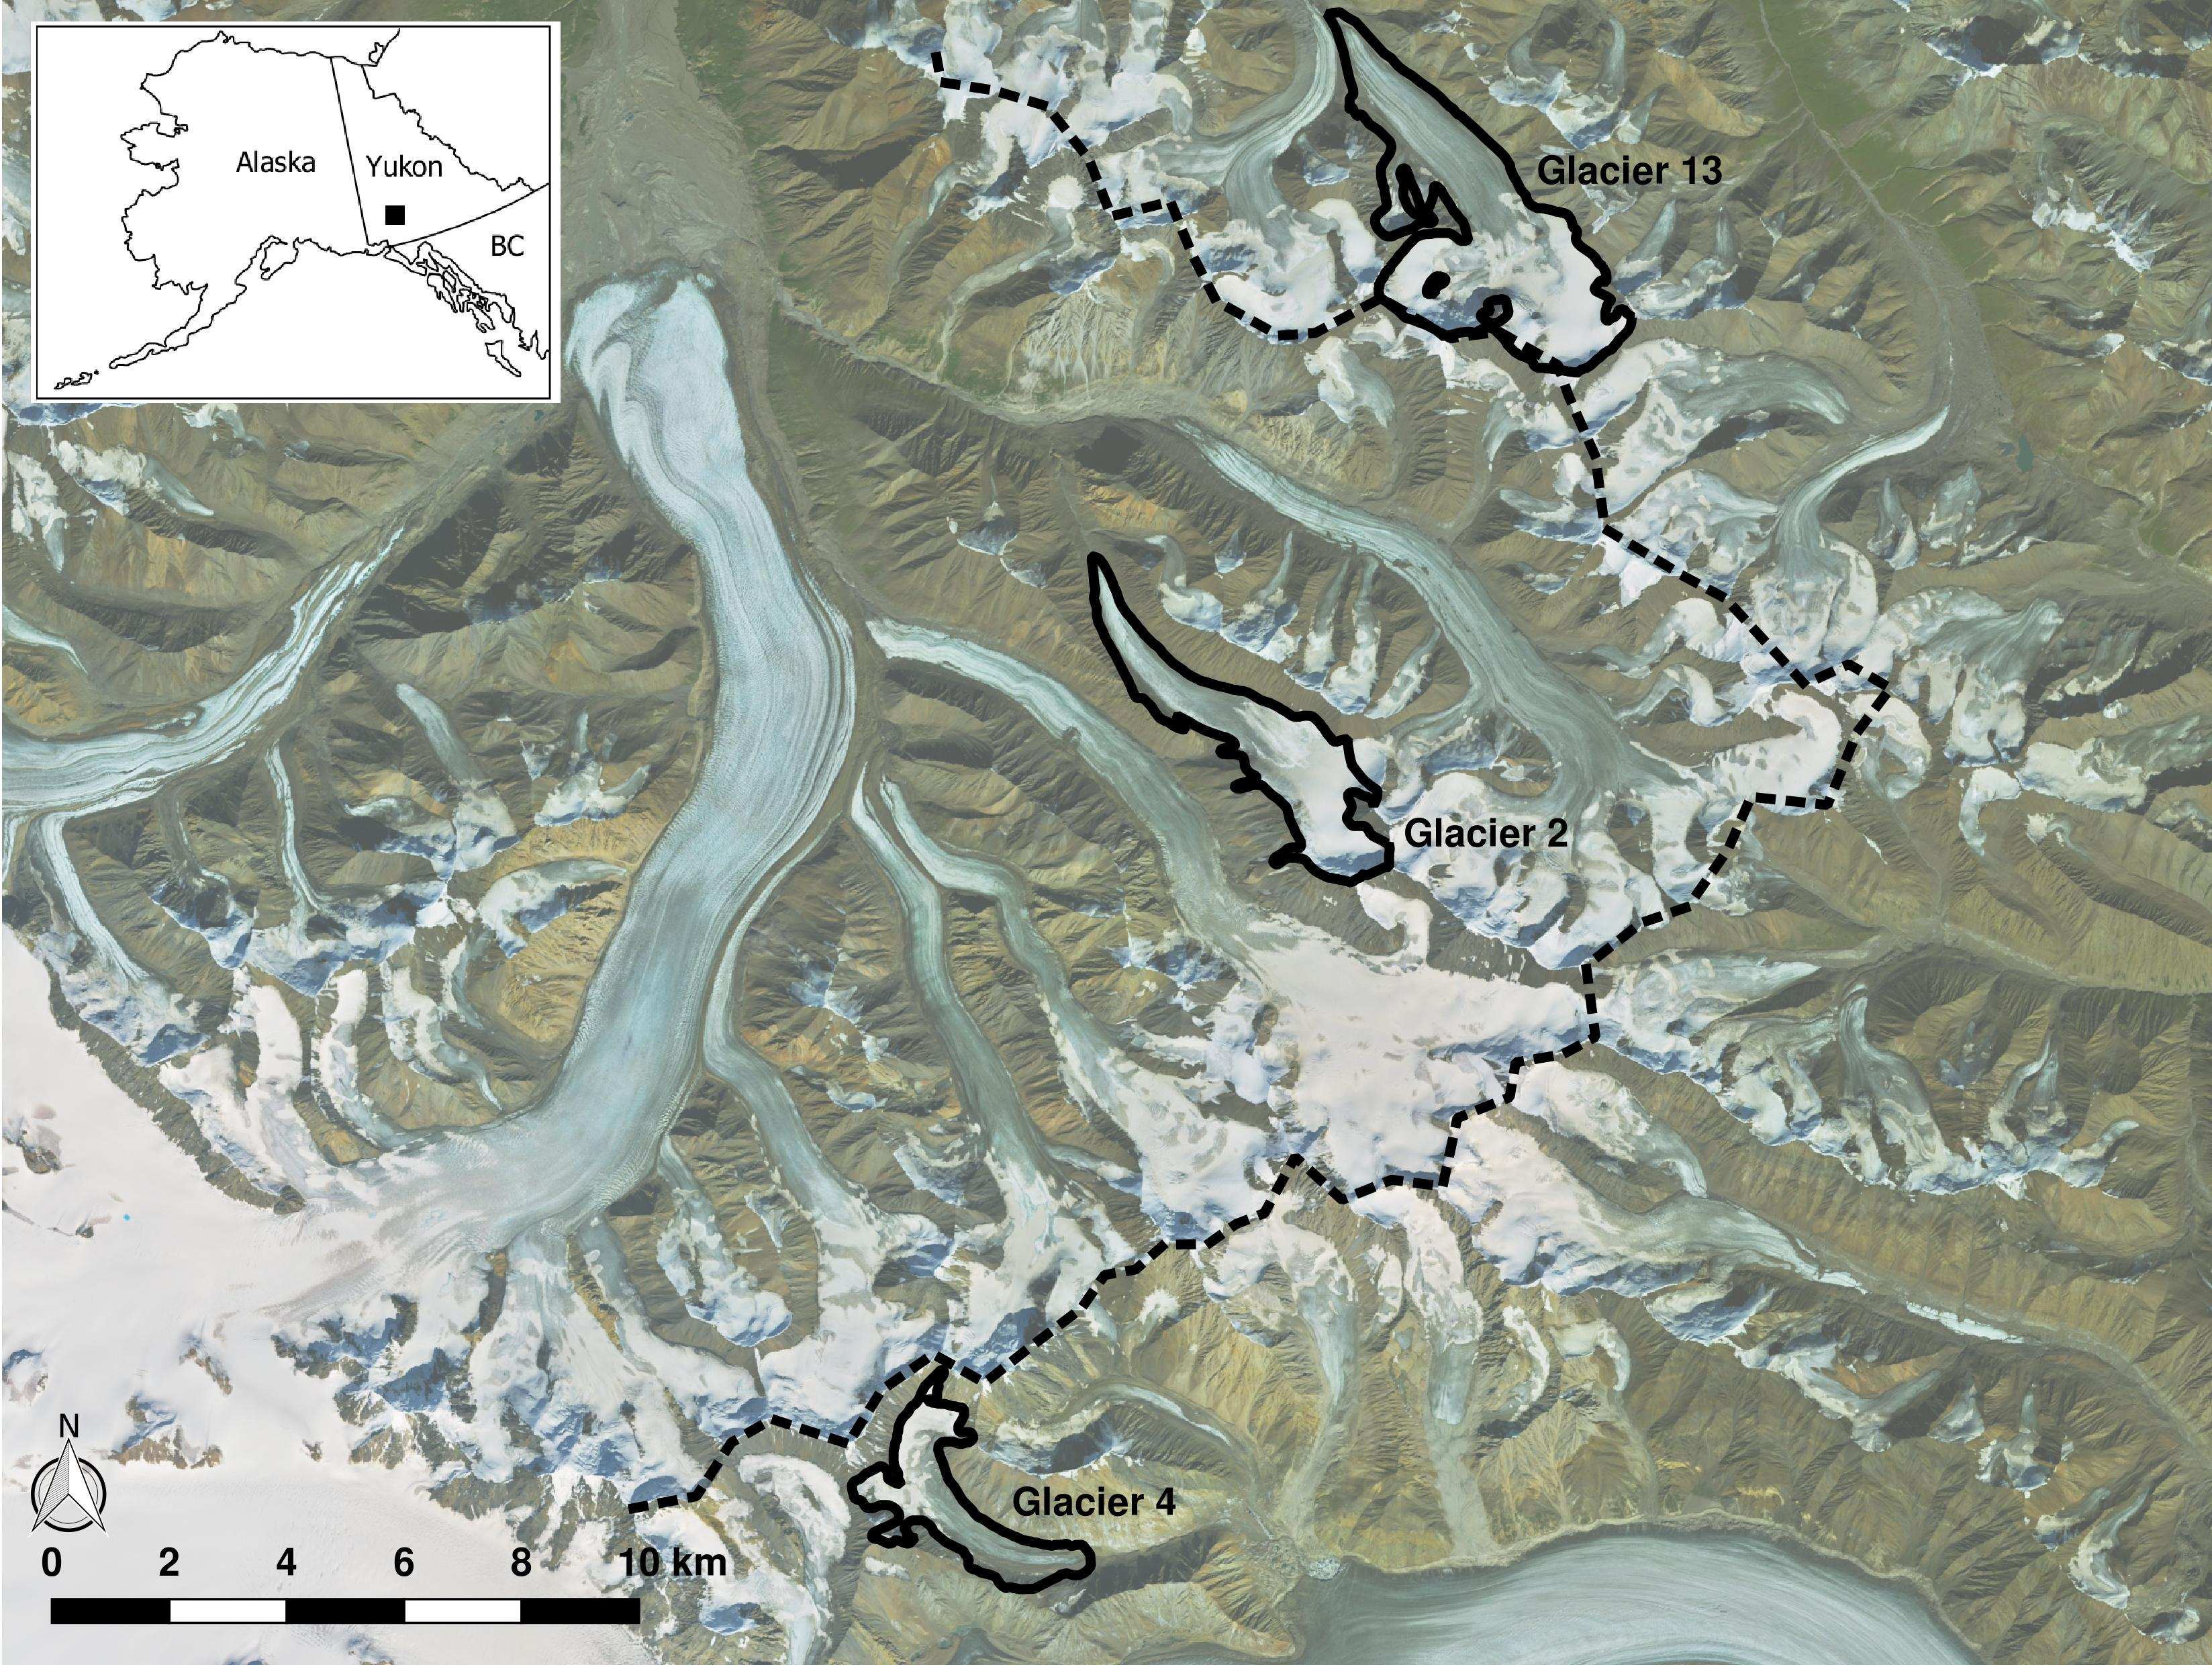
\includegraphics[width = \textwidth]{chosenglaciers.jpeg}}\\
	\caption{Study glaciers in the Donjek Range, Yukon (see inset). The local topographic divide is shown as a dashed line.}
	\label{studysites}
\end{figure}

\begin{figure}
	\centering
	\fbox{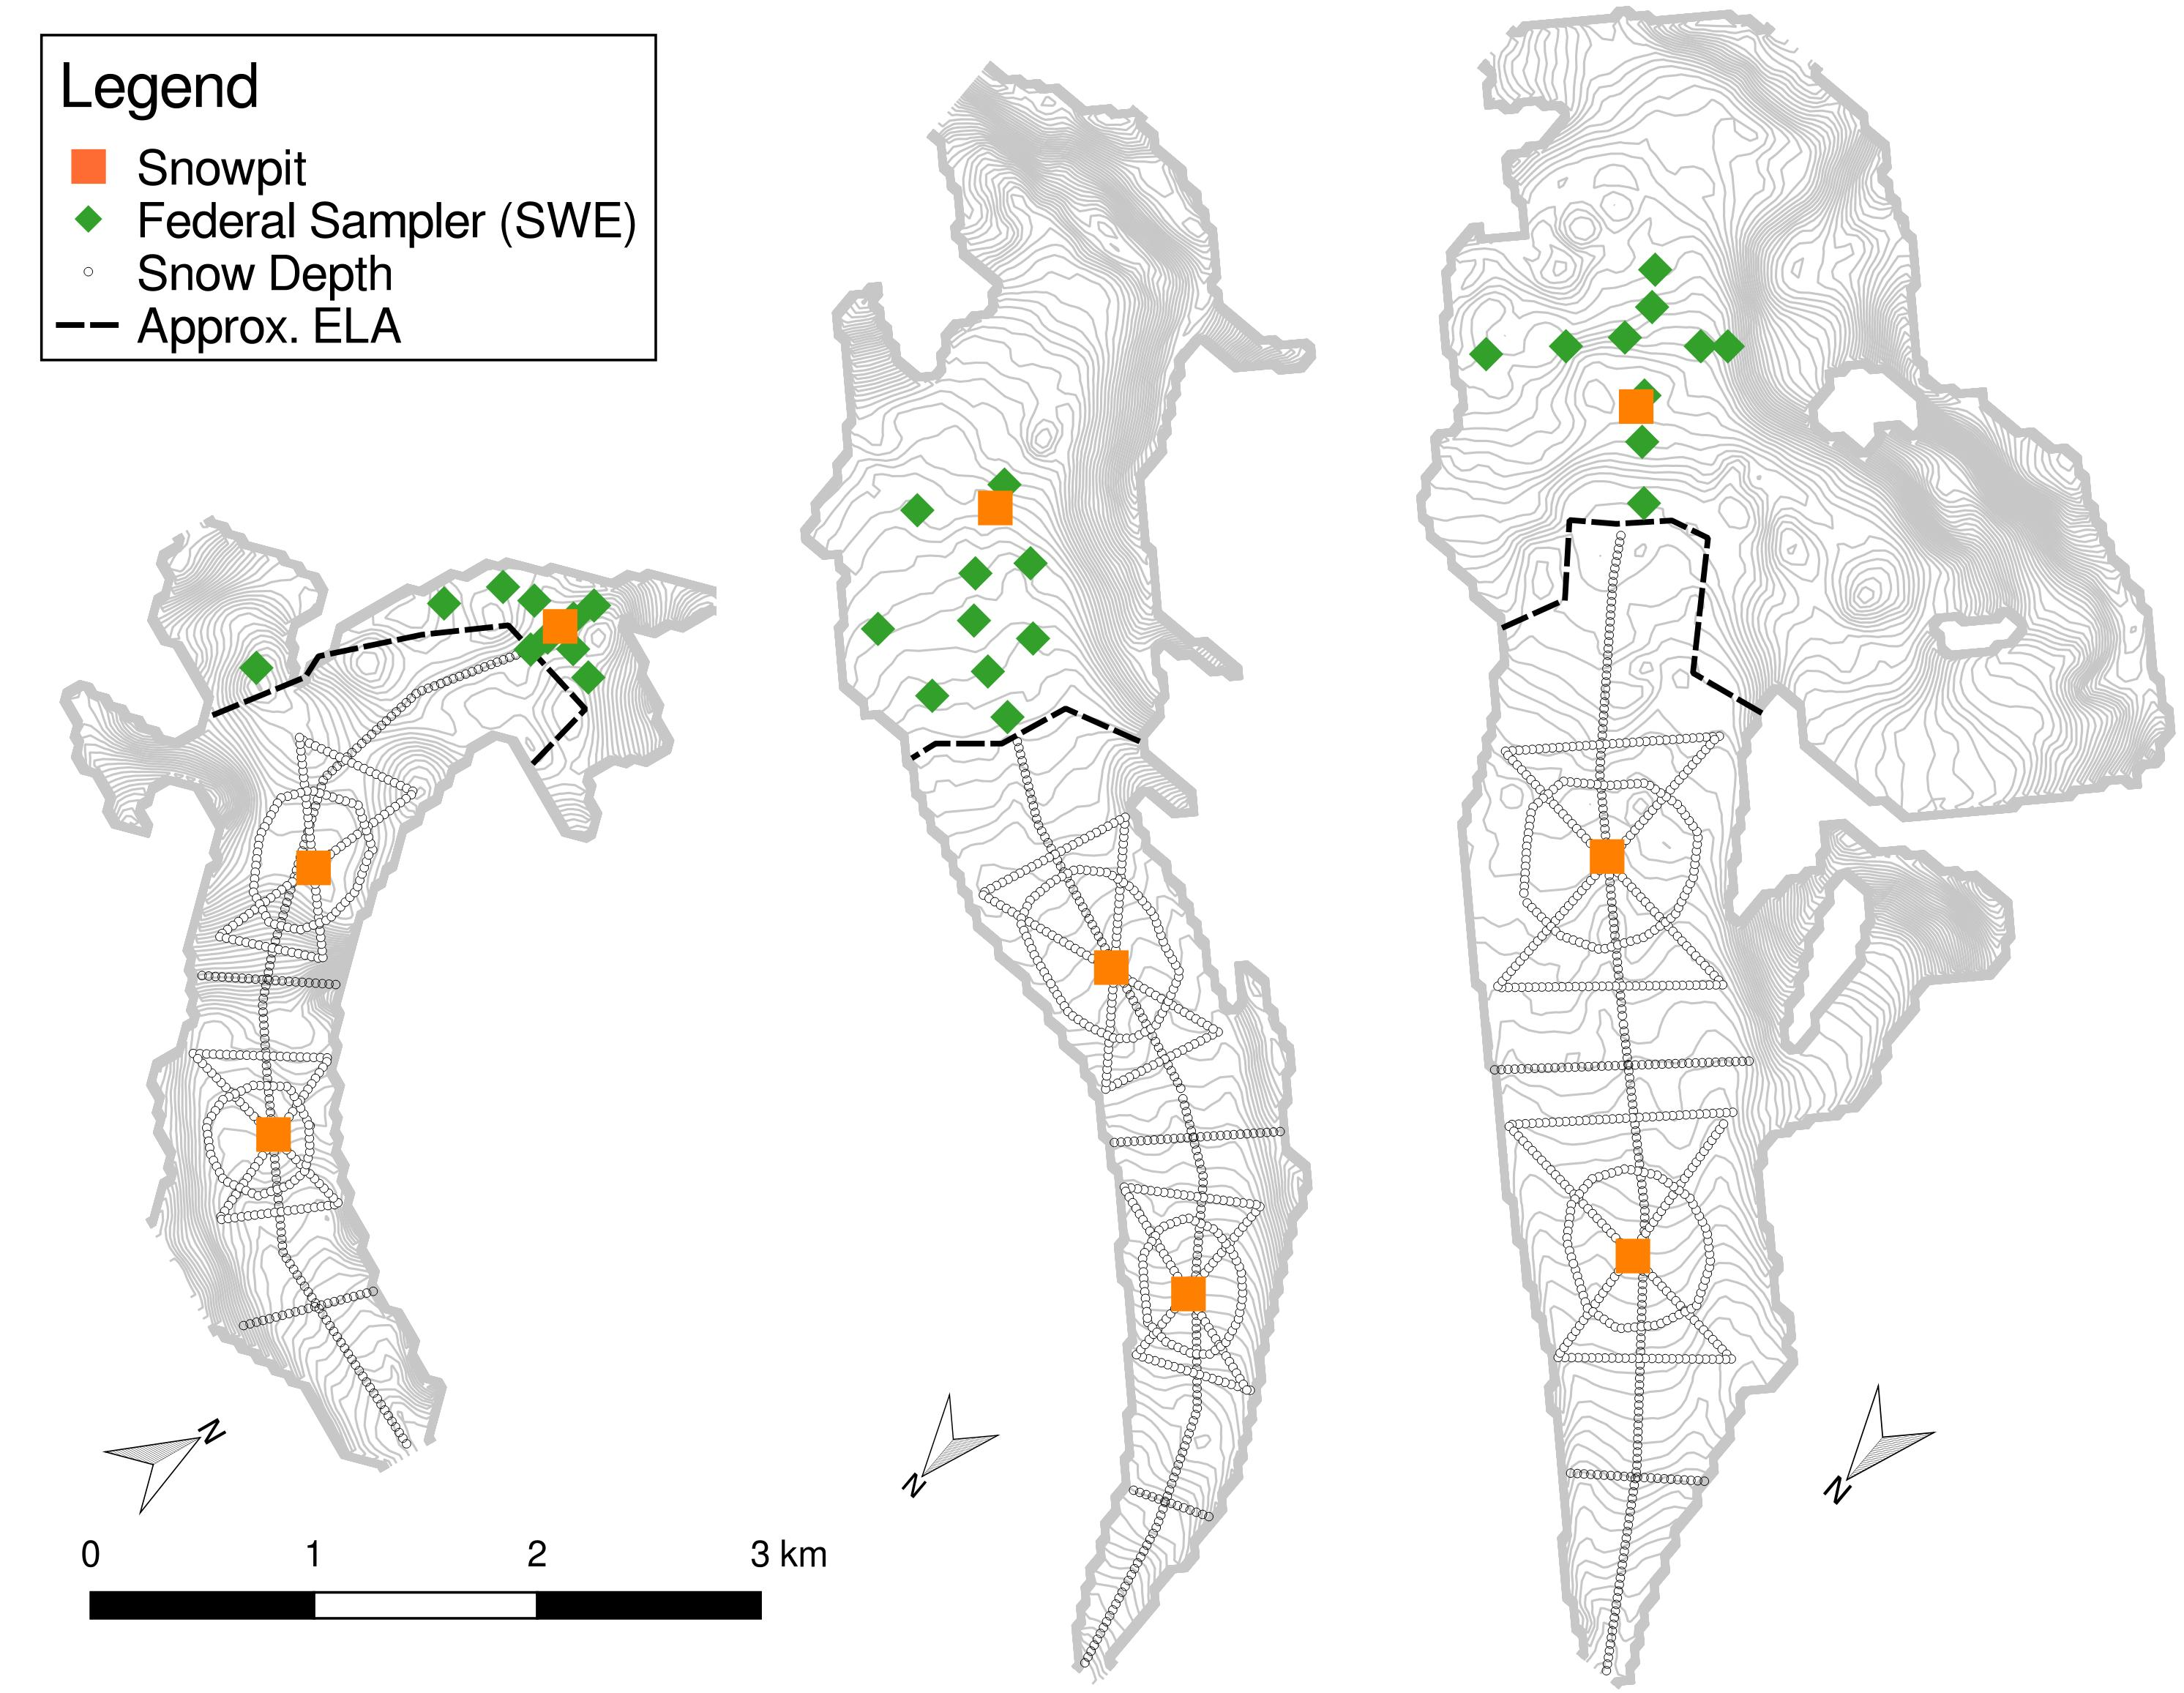
\includegraphics[width = \textwidth]{Transects_planned.jpeg}}\\
	\caption{Planned sampling design. Target waypoints for snow depth transects, snow pits and Federal Sampler measurements are shown for Glacier 4 (left), Glacier 2 (middle) and Glacier 13 (right).}
	\label{transect_planned}
	\end{figure}

\begin{figure}
	\centering
	\fbox{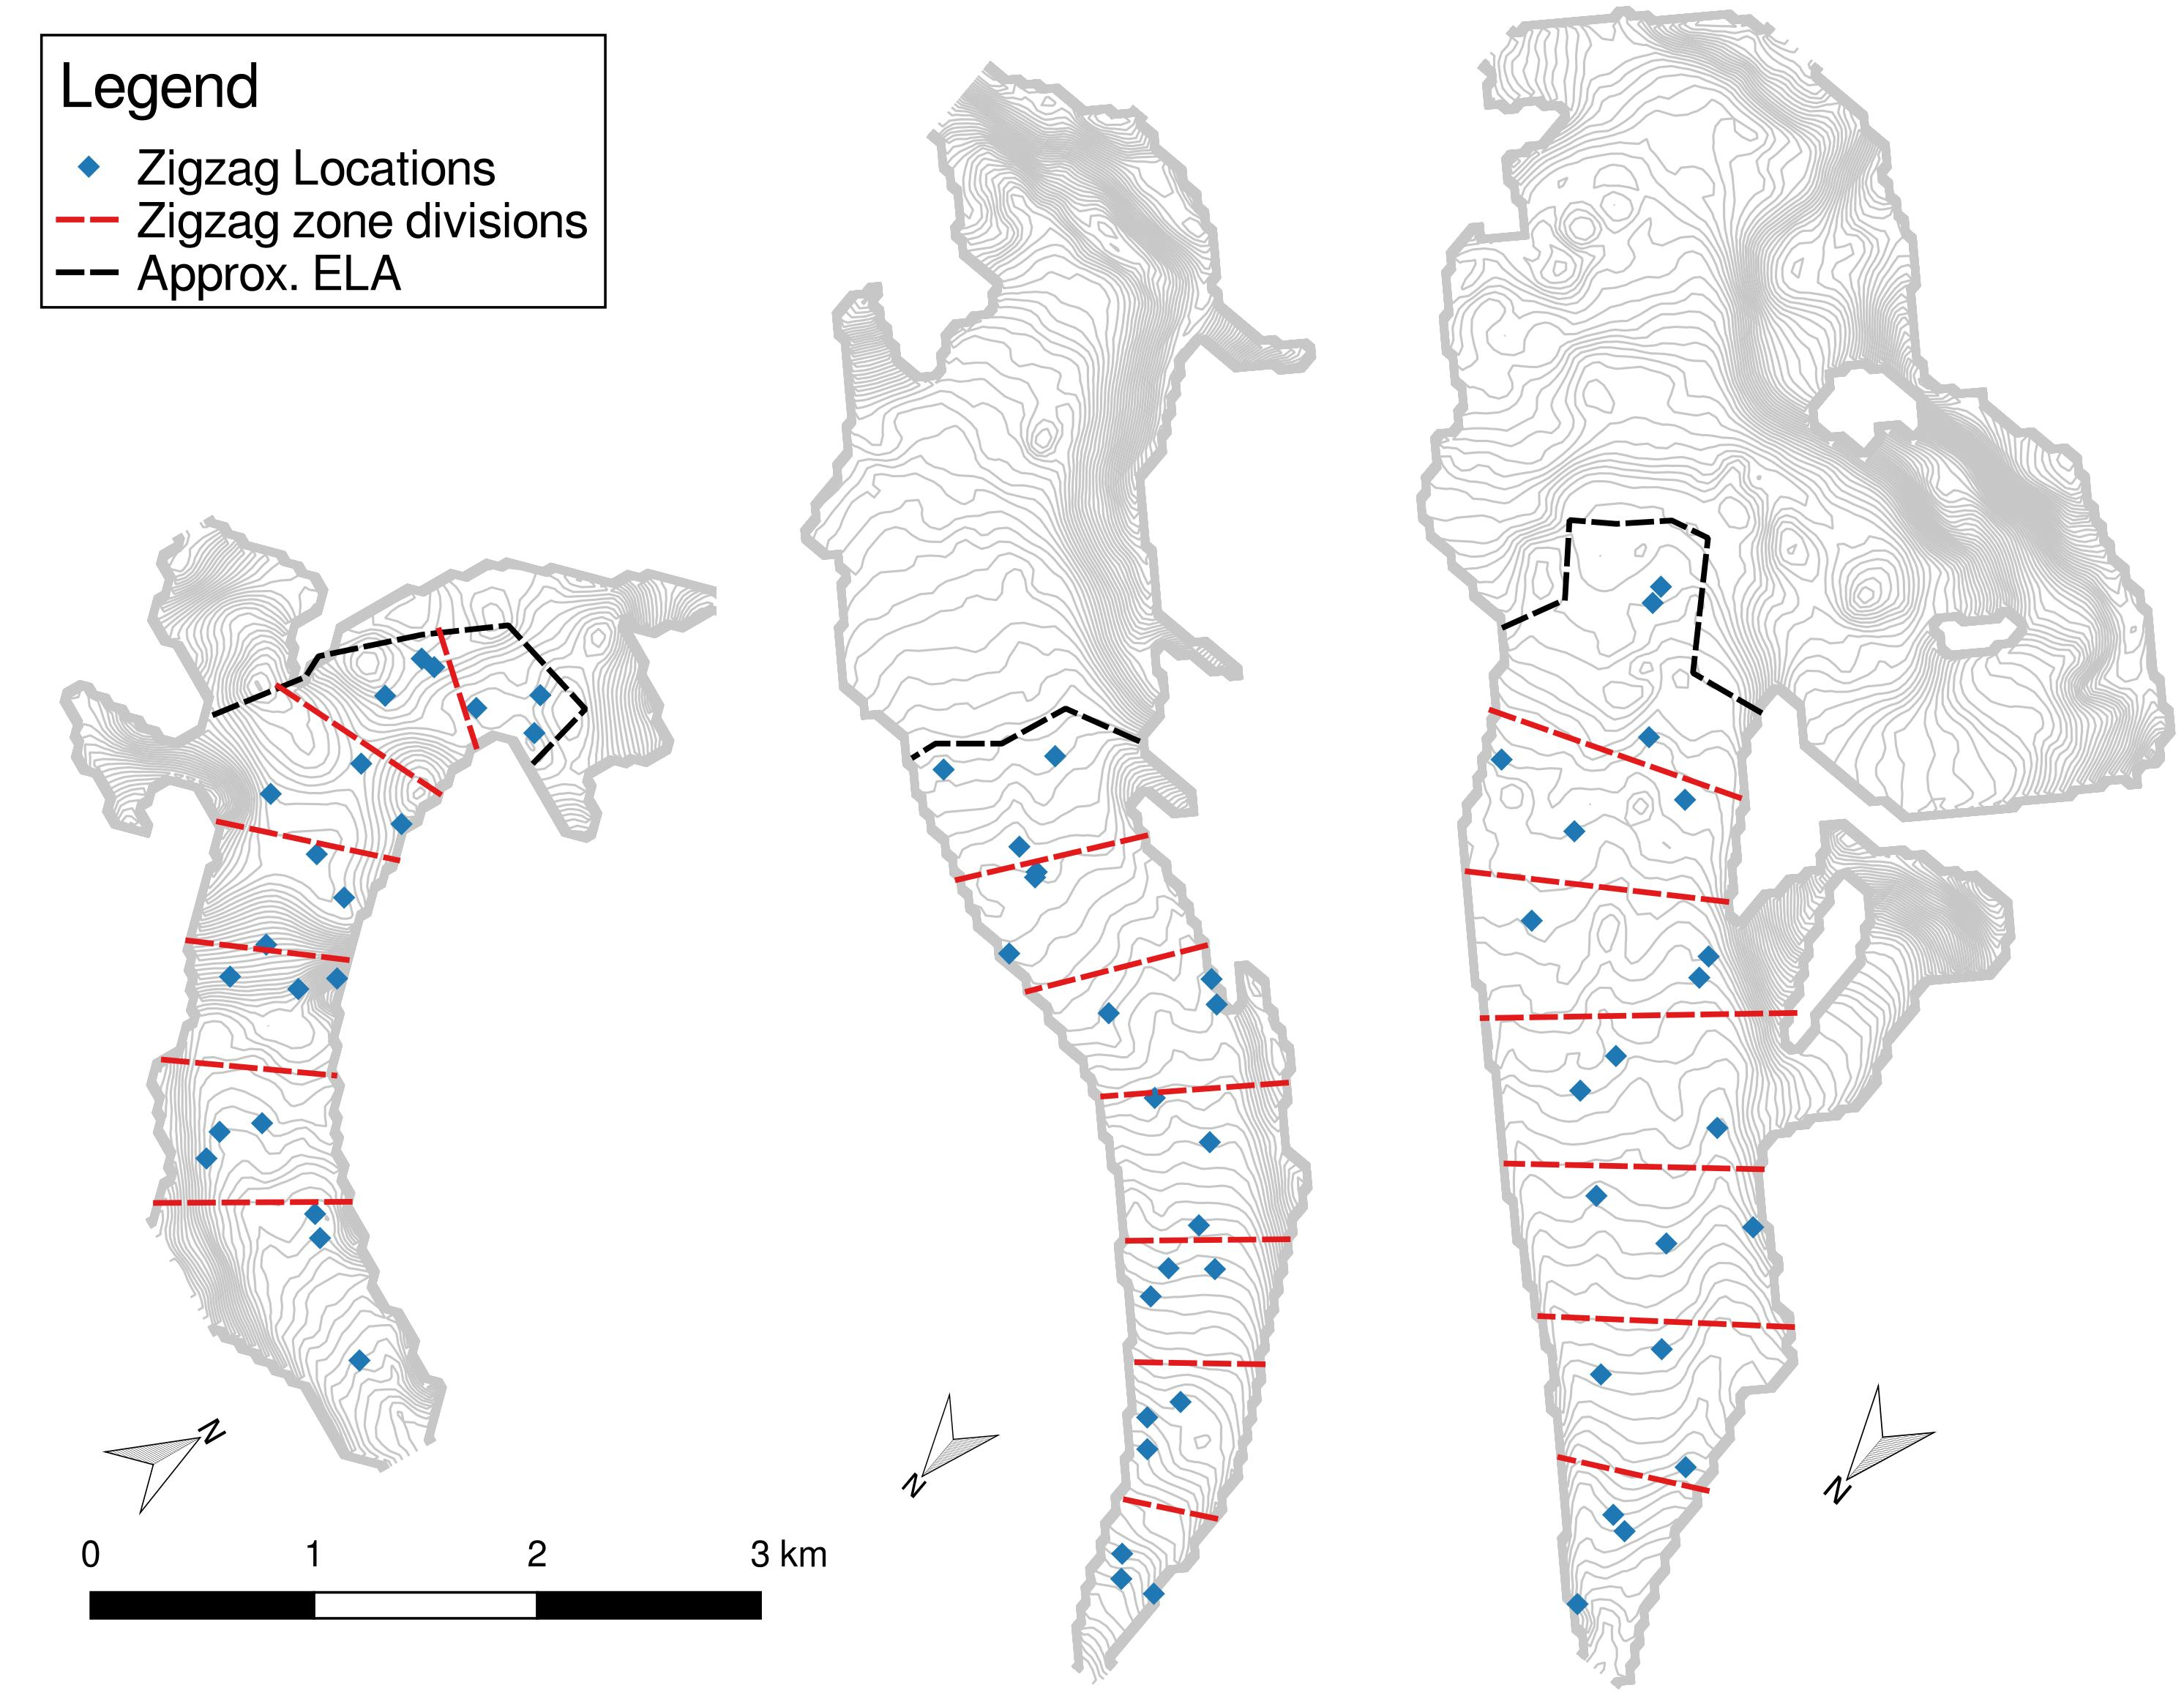
\includegraphics[width = \textwidth]{Zigzag_planned.jpeg}}\\
	\caption{Randomly assigned locations for zigzag measurements in the ablation areas (divided into seven zones) of Glacier 4 (left), Glacier 2 (middle) and Glacier 13 (right).}
	\label{zigzag_planned}
\end{figure}

\begin{figure}
	\centering
	\fbox{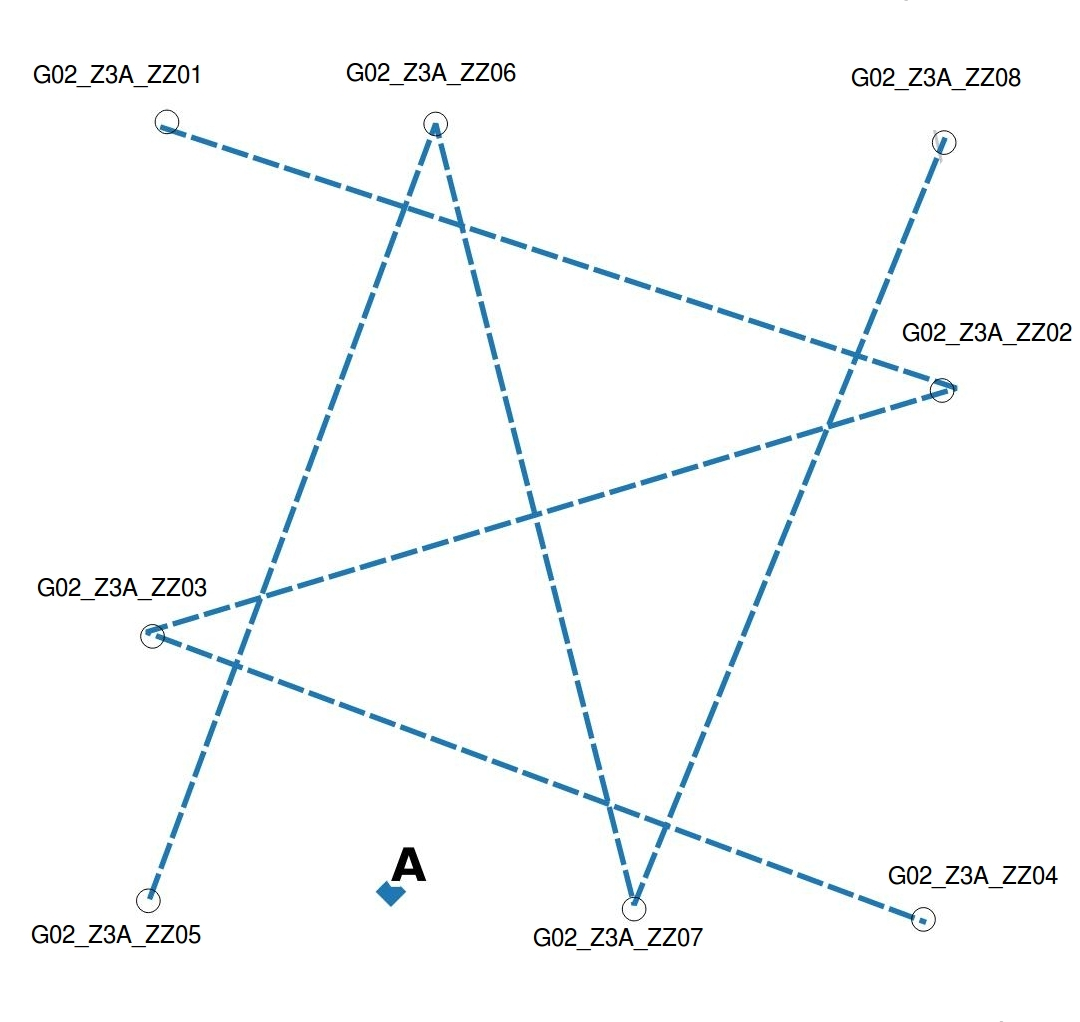
\includegraphics[width = 0.75\textwidth]{ZZ_vertex.jpeg}}\\
	\caption{Example of zigzag survey plan. Vertices are labelled and measurements are taken at random intervals along the dashed lines between vertices. The randomly chosen location of the Federal Sampler measurement is shown as a diamond.}
	\label{zigzag_vertex}
\end{figure}


%%%%
\section{Field methods}
%%%%

\subsection{Linear and Curvilinear Transects}
\label{sec:transects}

The transects, which include the hourglass, circle, transverse transect and midline, were all executed in a similar way. Along each transect, waypoints were marked every 30 m. To sample these locations, a team of four people was used in the configuration shown in Figure \ref{photo_probing} and schematically in Figure \ref{probing}. The four people were roped together so that during typical glacier travel there was approximately 10 m separating each person (likely ranged between 9.5 and 11 m). The front person was responsible for navigation and waypoint marking and would follow these steps for each measurement location:
\begin{enumerate}
\item Use the GPS device to locate each intended waypoint
\item Navigate to that location using the GPS device
\item Stop and inform the team when they had arrived at the location
\item Mark a new waypoint on the GPS device as the real location of the measurement (allow for auto labelling of waypoint, which was a three digit number that increased by one with subsequent waypoints). When needed, call out the waypoint label to the team.
\item In one line of a field book, write the labels `Intended' for the waypoint that was being navigated to (code created during planning stage), `Real' for the name of the newly created waypoint on the GPS device (three digit number), as well as the easting, northing and elevation for that location. This served as the backup for locating measurement points in the event of GPS device failure. 
\end{enumerate}

The remaining three people took snow depth measurement using graduated 3.2 m avalanche probes. Upon arriving at the waypoint they would follow these steps:
\begin{enumerate}
\item Insert the probe into the snow until the snow/ice interface was reached. Read the depth of the snow pack on the probe to 0.5\,cm. Repeat two (or three) more times (total of three (or four) measurements) within a 1 m$^2$ area of the first measurement and in a way that the three (or four) measurements are approximately equidistant. 
\item In one line of a field book, record the `Real' waypoint label (three digit number), as well as the three (or four) depth measurements. 
\end{enumerate}
Note that the snow/ice interface could often be differentiated from an ice lens. Typically, glacier ice felt hard, had a thin, low density snow layer above and created a bright `ping' sound in the probe. Ice lenses felt sticky and the probe would make a dull `thud' sound. In some locations this differentiation was obvious while in other locations it was difficult to determine what was at the end of the probe. Often, layers in the snowpack could be felt with the probe. For example, the probe would move easily through low density layers such as depth hoar and would `stick' to hard layers or ice lenses. Increasing the force applied to the probe would usually allow the probe to penetrate through hard layers. In cases where the `sticky' layer could not be penetrated, the observer would place a question mark next to the recorded depth or simply omit that measurement. A question mark was also placed beside measurements that were notably smaller than adjacent measurements. Note that the probe was inserted vertically, which was not necessarily perpendicular to the snow surface. The small, conical-shaped tip ($\sim$1\,cm) fell off most of the probes during field work. We were not able to determine when the tips fell off so no corrections were made to the snow depth measurements. 

It was originally planned for each observer to take four depth measurements in a square pattern. However, during the first transect the observers found it time consuming and difficult to remember and record four depths. The observers found that the most efficient way to collect data was to take three depth measurements, remember the values and then write them all down in the field book. Therefore, the number of measurements was reduced to three so that we could increase the number of locations measured. 

There were dedicated field books for each type of measurement rather than each observer. The first person had the `Navigation' field book, the second person had `Snow depth \#1', the third person had `Snow depth \#2' and the fourth person had `Snow depth \#3'. In this way, the location of each measured value can be inferred from its location relative to the navigation person (where the location was being recorded). For example, the `Snow depth \#3' value was located $\sim$30 m behind the waypoint location along the trajectory between the previous and current waypoint. This arrangement was preferred to having a field book for each observer because it minimized confusion and potential errors when entering and processing data.

In this arrangement, snow depth measurements could be taken every 10 m along a transect if a waypoint was marked every 30 m. For the first two transects, measurements were completed at every waypoint. However, this also proved to be too time consuming, so measurements were taken at every second waypoint for subsequent transects (exceptions include the midline on Glacier 4 and the lower hourglass on Glacier 2, see Table \ref{tab:snowdepthsummary}). A schematic of this arrangement can be seen in Figure \ref{probing:mapview}. Waypoints that were too dangerous to access were omitted. Additional waypoints (not originally uploaded to GPS devices) were created in some instances when travelling from the last accessible waypoint to the next accessible waypoint. A summary of information about the completed snow depth transects can be seen in Table \ref{tab:snowdepthsummary}.

\begin{figure}[H]
	\centering
	\fbox{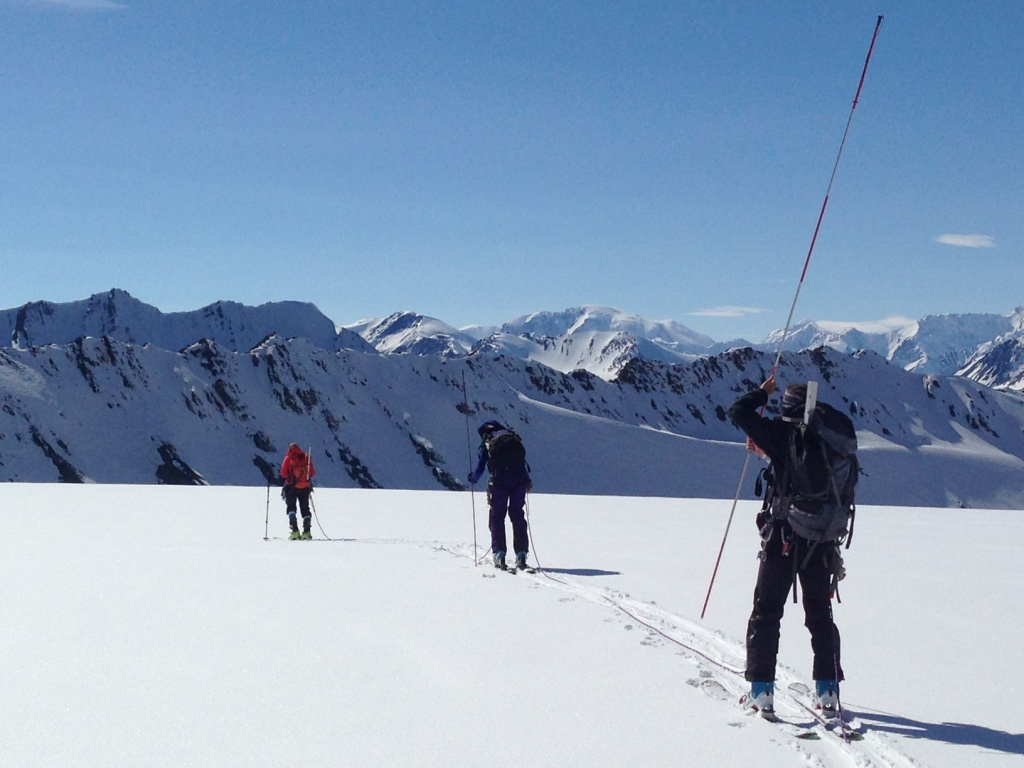
\includegraphics[width = 0.95\textwidth]{photo_probing.jpg}}\\
	\caption{Implementation of transect probing. The first person navigated to the intended waypoint using the GPS device. The second, third and fourth (not seen) observers are probing using 3.2 m long avalanche probes. There is approximately 10 m between observers. Photo credit: G. Flowers}
	\label{photo_probing}
	\end{figure}

\begin{figure}[H]
    \centering
    \begin{subfigure}[b]{0.8\textwidth}
        \fbox{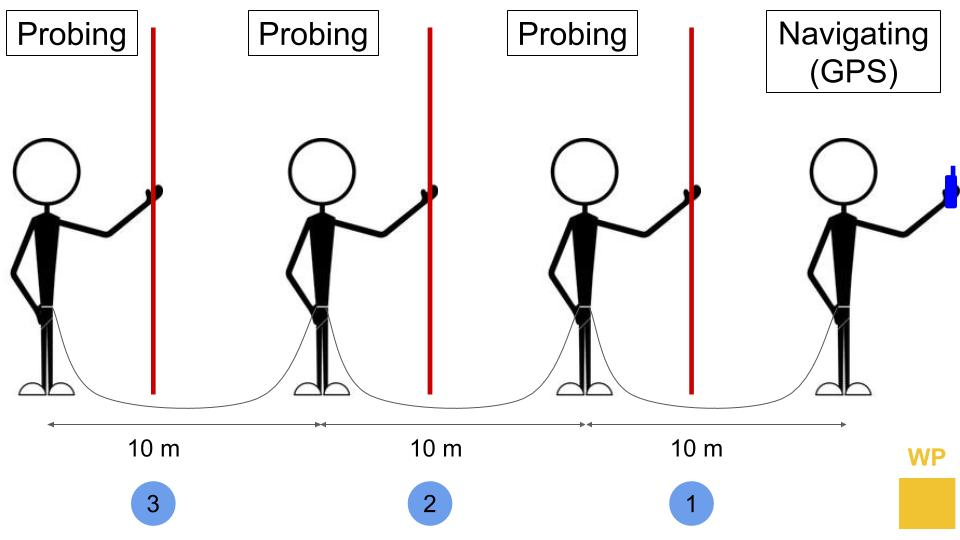
\includegraphics[width=\textwidth]{probers1.jpg}}
        \caption{Relative location of four people taking depth measurements at desired locations.}
        \label{probing:people}
    \end{subfigure}
    
    \begin{subfigure}[b]{0.8\textwidth}
        \fbox{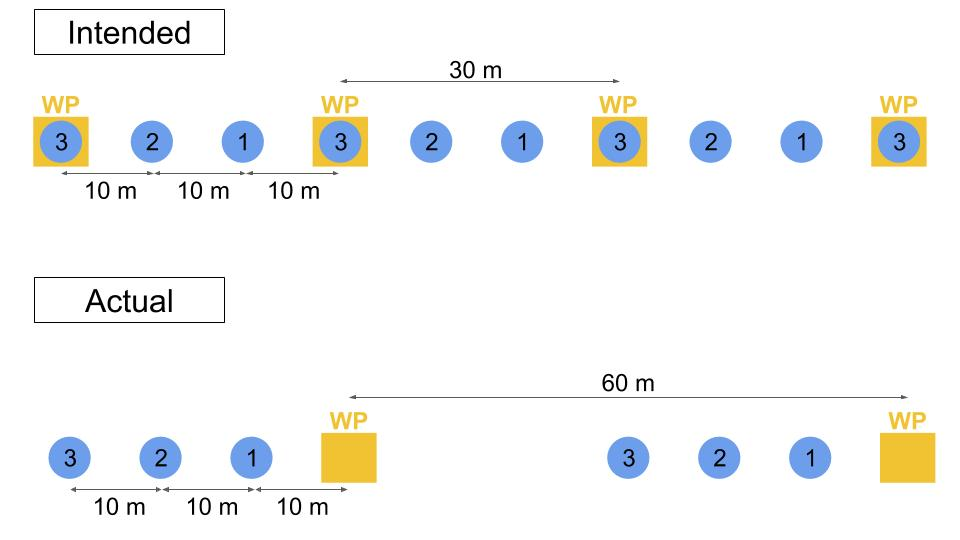
\includegraphics[width=\textwidth]{probers2.jpg}}
        \caption{Intended and actual transect-depth measurement spacing. In the intended design, there was uniform sample spacing along a transect with 10\,m sampling interval. In the actual implementation, every second waypoint was used so there were 60\,m between subsequent measurements.}
        \label{probing:mapview}
    \end{subfigure}

    \caption{Schematic of the snow depth measurement configuration. Blue circles indicate depth measurement and orange squares indicate waypoint (WP) locations.}\label{probing}
\end{figure}


\begin{sidewaystable}[]
\footnotesize
\centering
\caption{Summary information for snow depth transects. Transect shapes completed include Lower Hourglass (LH), Lower Circle (LC), Lower Midline (LM), Upper Hourglass (UH), Upper Circle (UC), Upper Midline (UM), Upper Transect (UT) and Bonus Transect (BT). The first observer navigated to waypoints and the remaining three made depth measurements. Observers given with initials of name.}
\label{tab:snowdepthsummary}
\begin{tabular}{ccccccl}

\textbf{Glacier}                                                             & \textbf{Shape}                                               & \textbf{\begin{tabular}[c]{@{}c@{}}Measurement\\ Interval\end{tabular}}  & \textbf{Date} & \textbf{\begin{tabular}[c]{@{}c@{}}GPS \\ Waypoint\\  Labels\end{tabular}} & \textbf{\begin{tabular}[c]{@{}c@{}}Observer\\  Order\end{tabular}} & \multicolumn{1}{c}{\textbf{Comments}}                                                                                                                                                                                                            \\ \hline
\multirow{7}{*}{\begin{tabular}[c]{@{}c@{}}Glacier 4\\ (G04)\end{tabular}}   & \textbf{LH}                                                  & \begin{tabular}[c]{@{}c@{}}30\,m \\ (60\,m for \\ upper part)\end{tabular} & 4 May 2016    & 021 -- 070                                                                 & GF--AP--CA--AC                                                     & \begin{tabular}[c]{@{}l@{}}4 depth measurement/location \\ along upper part\end{tabular}                                                                                                                                                         \\
                                                                             & \textbf{LC}                                                  & 60\,m                                                                     & 6 May 2016    & 159 -- 184                                                                 & GF--AP--CA--AC                                                     &                                                                                                                                                                                                                                                  \\
                                                                             & \textbf{LM}                                                  & 90\,m                                                                     & 7 May 2016    & 185 -- 207                                                                 & AP--GF--CA--AC                                                     &                                                                                                                                                                                                                                                  \\
                                                                             & \textbf{UH}                                                  & 60\,m                                                                     & 5 May 2016    & 072 -- 126                                                                 & CA--GF--AP--AC                                                     &                                                                                                                                                                                                                                                  \\
                                                                             & \textbf{UC}                                                  & 60\,m                                                                     & 5 May 2016    & 127 -- 157                                                                 & CA--GF--AP--AC                                                     &                                                                                                                                                                                                                                                  \\
                                                                             & \textbf{UM}                                                  & 90\,m                                                                     & 7 May 2016    & 208 -- 221                                                                 & AP--GF--CA--AC                                                     & Additional measurement at WP 158 (6 May 2016)                                                                                                                                                                                                               \\
                                                                             & \textbf{UT}                                                  & 30\,m                                                                     & 4 May 2016    & 004 -- 020                                                                 & GF--AP--CA--AC                                                     & 4 depth measurement/location                                                                                                                                                                                                                     \\ \hline
\multirow{7}{*}{\begin{tabular}[c]{@{}c@{}}Glacier 2 \\ (G02)\end{tabular}}  & \textbf{\begin{tabular}[c]{@{}c@{}}LH \\ \& LC\end{tabular}} & 30\,m                                                                     & 11 May 2016   & 371 -- 518                                                                 & GF--AP--CA                                                         & \begin{tabular}[c]{@{}l@{}}Only two probers. Avoided crossing main \\ channel so LH \& LC were combined and \\ done together on glacier right and then \\ glacier left of the channel.\end{tabular} \\
                                                                             & \textbf{LM}                                                  & $\sim$60\,m                                                               & 10 May 2016   & 355 -- 370                                                                 & AP--GF--CA--AC                                                     & \begin{tabular}[c]{@{}l@{}}Original points along supraglacial stream \\ bed so points moved to glacier right and \\ locations were approximated\end{tabular}                                                                                     \\
                                                                             & \textbf{UH}                                                  & 60\,m                                                                     & 8 May 2016    & 223 -- 275                                                                 & AC--AP--CA--GF                                                     & \begin{tabular}[c]{@{}l@{}}Many corner points avoided due to \\ crevasse danger\end{tabular}                                                                                                                                                     \\
                                                                             & \textbf{UC}                                                  & 60\,m                                                                     & 8 May 2016    & 276 -- 313                                                                 & AC--AP--CA--GF                                                     &                                                                                                                                                                                                                                                  \\
                                                                             & \textbf{UM}                                                  & 60\,m                                                                     & 9 May 2016    & 313 -- 343                                                                 & AC--AP--CA--GF                                                     &                                                                                                                                                                                                                                                  \\
                                                                             & \textbf{UT}                                                  & 60\,m                                                                     & 11 May 2016   & 519 -- 528                                                                 & GF--AP--CA                                                         & Only two probers                                                                                                                                                                                                                                 \\
                                                                             & \textbf{BT}                                                  & $\sim$60\,m                                                               & 19 May 2016   & 344 -- 354                                                                 & GF--AP--CA--AC                                                     &                                                                                                                                                                                                                                                  \\ \hline
\multirow{7}{*}{\begin{tabular}[c]{@{}c@{}}Glacier 13 \\ (G13)\end{tabular}} & \textbf{LH}                                                  & 60\,m                                                                     & 15 May 2016   & 745 -- 811                                                                 & AC--AP--CA--GF                                                     &                                                                                                                                                                                                                                                  \\
                                                                             & \textbf{LC}                                                  & 60\,m                                                                     & 15 May 2016   & 812 -- 847                                                                 & AC--AP--CA--GF                                                     &                                                                                                                                                                                                                                                  \\
                                                                             & \textbf{LM}                                                  & 60\,m                                                                     & 14 May 2016   & 714 -- 743                                                                 & AC--AP--CA--GF                                                     &                                                                                                                                                                                                                                                  \\
                                                                             & \textbf{UH}                                                  & 60\,m                                                                     & 12 May 2016   & 571 -- 650                                                                 & AC--GF--CA--AP                                                     &                                                                                                                                                                                                                                                  \\
                                                                             & \textbf{UC}                                                  & 60\,m                                                                     & 12 May 2016   & 529 -- 570                                                                 & AC--GF--CA--AP                                                     &                                                                                                                                                                                                                                                  \\
                                                                             & \textbf{UM}                                                  & 60\,m                                                                     & 14 May 2016   & 678 -- 713                                                                 & AC--AP--CA--GF                                                     &                                                                                                                                                                                                                                                  \\
                                                                             & \textbf{UT}                                                  & 60\,m                                                                     & 14 May 2016   & 660 -- 677                                                                 & AC--AP--CA--GF                                                     &                                                                                                                                                                                                                                                 
\end{tabular}
\end{sidewaystable}


\begin{sidewaystable}[]
\normalsize
\centering
\caption{Summary information for zigzag measurements. Observers given with initials of name.}
\label{tab:zigzagsummary}
\begin{tabular}{ccccccl}
\textbf{Glacier} & \textbf{Zone} & \textbf{Priority} & \textbf{Date} & \textbf{Observers} & \textbf{\begin{tabular}[c]{@{}c@{}}Number of\\ Measurements\end{tabular}} & \multicolumn{1}{c}{\textbf{Comments}}                                                                          \\ \hline
G04              & 3             & A                 & 5 May 2016    & AP/CA  &168            &                                                                                                                \\
G04              & 2             & A                 & 7 May 2016    & CA/AC   &135           &                                                                                                                \\
G04              & 5             & B                 & 7 May 2016    & AP/GF  &146            & \begin{tabular}[t]{@{}l@{}}Sticky layer - many points not collected\\ Snowing during measurements\end{tabular} \\ \hline
G02              & 5             & C                 & 10 May 2016   & CA/GF   &152           & \begin{tabular}[t]{@{}l@{}}Extra line measured\\ Vertex labelling error in GPS device \end{tabular}                                                                                   \\
G02              & 7             & A                 & 10 May 2016   & CA/GF/AP/AC   &191           & \begin{tabular}[t]{@{}l@{}}Channel present\\ Vertex labelling error in GPS device\end{tabular}                        \\
G02              & 3             & B                 & 10 May 2016   & GF/AP   &160           & Vertex labelling error in GPS device                                                                                  \\ \hline
G13              & 7             & C                 & 14 May 2016   & AC/AP  &167            & Vertex labelling error in GPS device                                                                                  \\
G13              & 4             & C                 & 14 May 2016   & GF/CA   &143           & \begin{tabular}[t]{@{}l@{}}Channel present\\ Vertex labelling error in GPS device\end{tabular}                        \\
G13              & 3             & B                 & 15 May 2016   & GF/CA    &164          & Vertex labelling error in GPS device                                                                                  \\
G13              & 5             & A                 & 15 May 2016   & AP/AC   &157           & \begin{tabular}[t]{@{}l@{}}Mushy snow that collapses\\ Vertex labelling error in GPS device\end{tabular}             
\end{tabular}
\end{sidewaystable}


 \begin{figure}[H]
	\centering
	\fbox{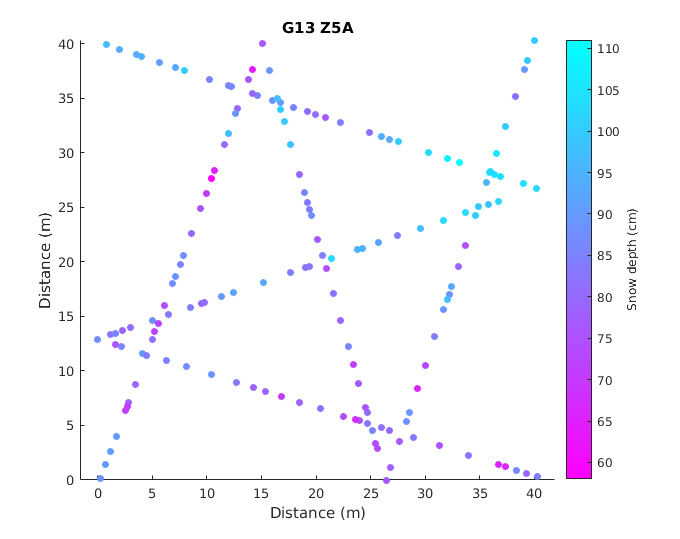
\includegraphics[width = 0.9\textwidth]{zigzag_completed.png}}\\
	\caption{Snow depth values measured along a zigzag pattern (G04\_Z3A)}
	\label{zigzag_example}
\end{figure}


\begin{table}[]
\small
\centering
\caption{Summary information for Federal Sampler measurements }
\label{tab:SWEsummary}
\begin{tabular}{ccccccl}
\textbf{Glacier}      & \textbf{Location} & \textbf{\begin{tabular}[c]{@{}c@{}}Total \\ number of \\ samples \end{tabular}} & \textbf{\begin{tabular}[c]{@{}c@{}}Number \\ of tube \\ lengths\end{tabular}} & \textbf{Date} & \textbf{Observers} & \multicolumn{1}{c}{\textbf{Comments}}  \\ \hline
\multirow{7}{*}{G04}  & Z3A & 5    & 3 & 5 May 2016    & GF/AC   &  \\
                      & USP               & 9                                                         & 3                                                                             & 5 May 2016    & GF/CA              &                                                                              \\
                      & Z2A               & 3                                                               & 3                                                                             & 7 May 2016    & GF/AP              &                                                                              \\
                      & LSP               & 9                                                        & 3                                                                             & 7 May 2016    & GF/CA              &                                                                              \\
                      & Z5B               & 3                                                               & 3                                                                             & 7 May 2016    & CA/AC              &                                                                              \\
                      & Z5A               & 3                                                               & 3                                                                             & 7 May 2016    & CA/AC              &                                                                              \\
                      & Z5C               & 3                                                               & 2                                                                             & 7 May 2016    & CA/AC              &                                                                              \\ \hline
\multirow{7}{*}{G02}  & Z5C               & 3                                                               & 2                                                                             & 10 May 2016   & AP/AC              &                                                                              \\
                      & USP               & 9                                                         & 2                                                                             & 10 May 2016   & AP/AC              &                                                                              \\
                      & Z7A               & 3                                                               & 3                                                                             & 10 May 2016   & CA/GF              &                                                                              \\
                      & Z7B               & 3                                                               & 3                                                                             & 10 May 2016   & CA/GF              &                                                                              \\
                      & Z7C               & 3                                                               & 2                                                                             & 10 May 2016   & AP/CA              &                                                                              \\
                      & LSP               & 8                                                         & 1                                                                             & 10 May 2016   & CA/AC              & \begin{tabular}[t]{@{}l@{}}Used snow pit \\ spring scale (grams)\end{tabular} \\
                      & Z3B               & 3                                                               & 1                                                                             & 10 May 2016   & CA/AC              & \begin{tabular}[t]{@{}l@{}}Used snow pit \\ spring scale (grams)\end{tabular} \\ \hline
\multirow{19}{*}{G13} & ASP               & 8                                                         & 3                                                                             & 13 May 2016   & AP/AC              &                                                                              \\
                      & AFC05             & 3                                                               & 3                                                                             & 13 May 2016   & AP/CA              & \begin{tabular}[t]{@{}l@{}}Probe depth \\ $\neq$ tube depth\end{tabular}     \\
                      & WP 651            & 3                                                               & 3                                                                             & 13 May 2016   & AP/CA/GF           &                                                                              \\
                      & WP 652            & 4                                                               & 3                                                                             & 13 May 2016   & AP/CA/GF           &                                                                              \\
                      & WP 653            & 3                                                               & 3                                                                             & 13 May 2016   & AP/CA/GF           &                                                                              \\
                      & WP 654            & 3                                                               & 3                                                                             & 13 May 2016   & AP/CA/GF           &                                                                              \\
                      & WP 655            & 3                                                               & 3                                                                             & 13 May 2016   & AP/CA/GF           &                                                                              \\
                      & WP 656            & 3                                                               & 3                                                                             & 13 May 2016   & AP/CA/GF           &                                                                              \\
                      & WP 657            & 3                                                               & 3                                                                             & 13 May 2016   & AP/CA/GF           &                                                                              \\
                      & WP 658            & 3                                                               & 3                                                                             & 13 May 2016   & AP/CA/GF           &                                                                              \\
                      & WP 659            & 3                                                               & 3                                                                             & 13 May 2016   & AP/CA/GF           &                                                                              \\
                      & Z7C               & 3                                                               & 2                                                                             & 13 May 2016   & CA/GF              &                                                                              \\
                      & USP               & 8                                                         & 2                                                                             & 14 May 2016   & AP/AC              & \begin{tabular}[t]{@{}l@{}}Ice layer near \\ bottom\end{tabular}             \\
                      & Z4C               & 3                                                               & 3                                                                             & 14 May 2016   & AP                 & In stream channel                                                            \\
                      & WP 744            & 3                                                               & 2                                                                             & 14 May 2016   & AP                 & In Z4C zigzag                                                                \\
                      & Z3B               & 3                                                               & 2                                                                             & 15 May 2016   & AP/AC              &                                                                              \\
                      & Z4B               & 3                                                               & 2                                                                             & 15 May 2016   & AP/AC              &                                                                              \\
                      & Z5C               & 3                                                               & 2                                                                             & 15 May 2016   & CA/GF              &                                                                              \\
                      & Z5B               & 3                                                               & 2                                                                             & 15 May 2016   & CA/AC              &                                                                             
\end{tabular}
\end{table}



\subsection{Zigzag survey}
\label{sec:zigzagmethods}

The zigzag sampling pattern was used to obtain many measurements within a 40$\times$40\,m area.  The pattern consisted of two intersecting `Z'-shaped transects. Snow depth was measured with random spacing between 0.3\,m and 3.0\,m. 

Two teams of two people were used to complete each zigzag. The first team would navigate to the vertices of the zigzag using the GPS device and place wands at each vertex. Often the tracks would not be straight between two vertices so the second team would use the wands to travel between vertices in as straight a line as possible. The first person would use the avalanche probe to measure out the distance to the next measurement spot and then probe at that point (Sturm, M., 2016 personal communication). Probing protocol was exactly the same as for transect measurements but only measurement was made at each location (see Section \ref{sec:transects}). The first person would call out the depth to the second person, who was responsible for recording the distance between measurements and the depth at the measurement point. A field book was dedicated to zigzag measurements and each page would have the name of the vertex where measurements started, the distance from the previous measurement point and the depth at that point. The second person also had a sheet with random numbers from a uniform distribution between 0.3 and 3.0 m (generated using Matlab) and would call out these numbers in order as the distance between measurement points. While the second team was measuring snow depth, the first team used a Federal Sampler to take three snow water equivalent measurements with a $\sim$1 m area around the predetermined location within the zigzag area (see Section \ref{sec:SWE} for protocol). An example of a completed zigzag pattern can be seen in Figure \ref{zigzag_example} and a summary of information about completed zigzags can be found in Table \ref{tab:zigzagsummary}.  


 \subsection{Federal Snow Sampler}
\label{sec:SWE}
 
\begin{figure}[H]
    \centering
    \begin{subfigure}[b]{0.39\textwidth}
        \fbox{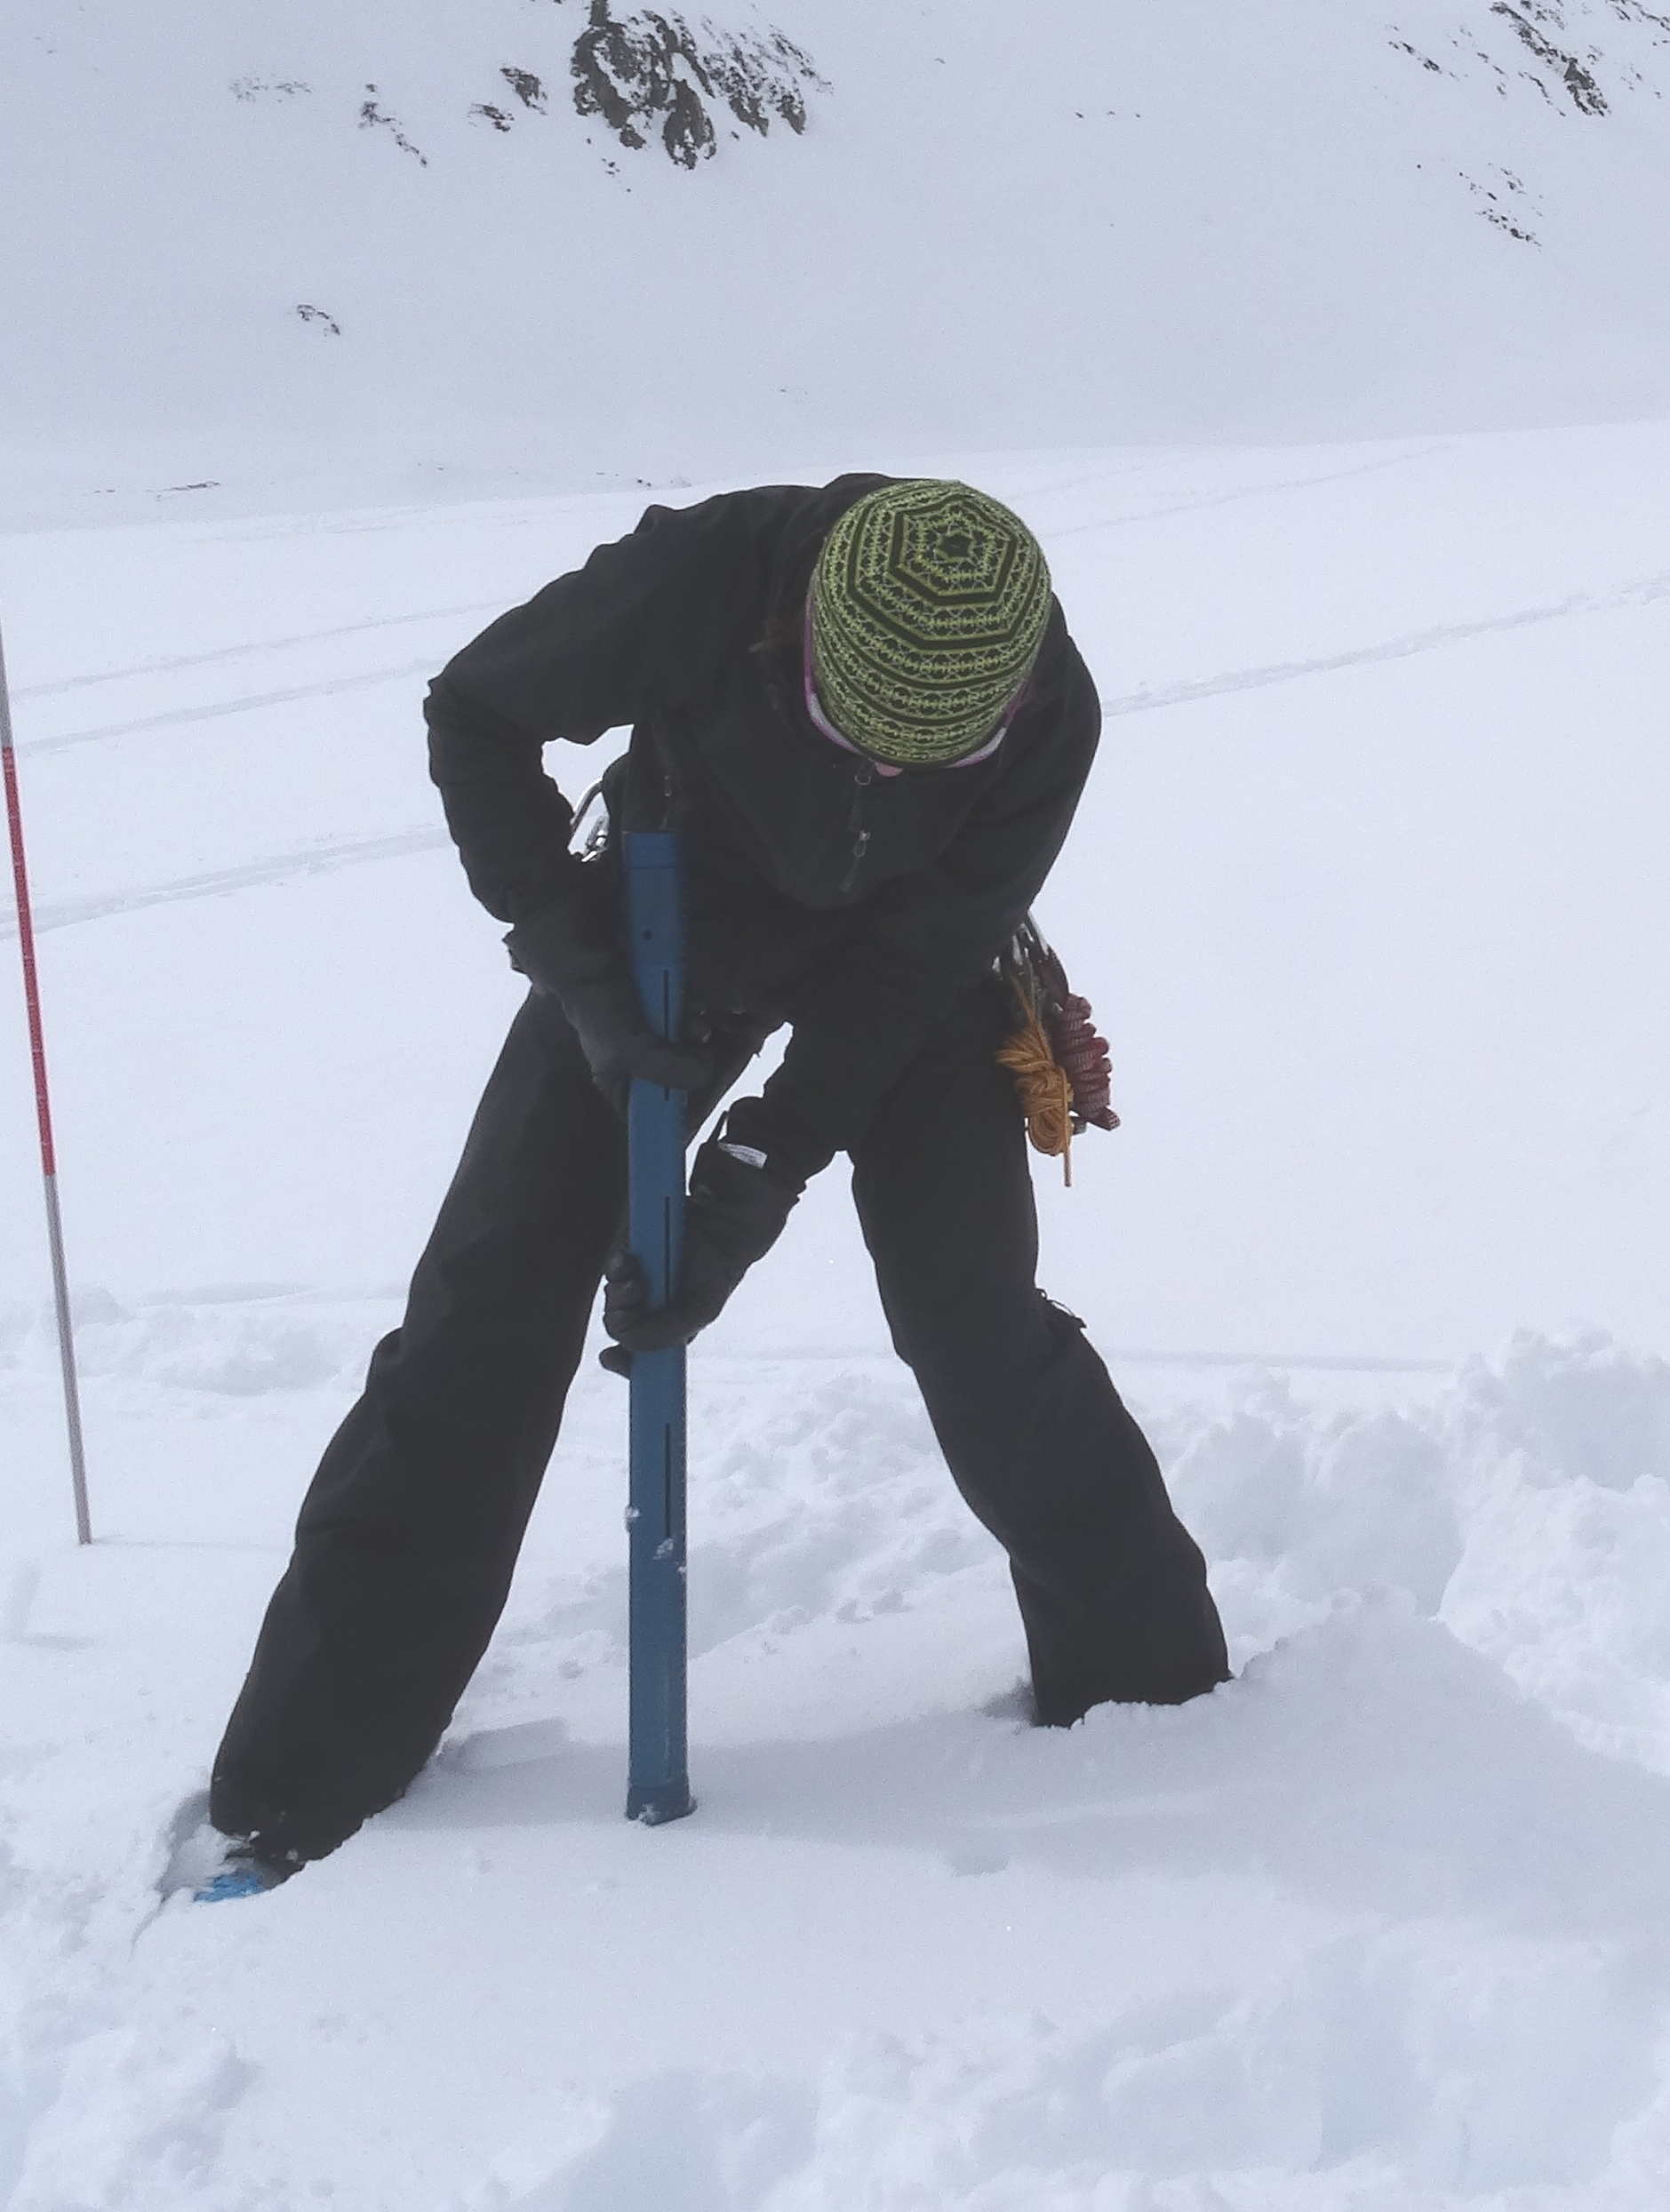
\includegraphics[width=\textwidth]{photo_swe1.JPG}}
        \caption{Inserting the Federal Sampler into the snow. Photo credit: C. Ariagno}
        \label{photo_swe1}
    \end{subfigure}
    ~
    \begin{subfigure}[b]{0.55\textwidth}
        \fbox{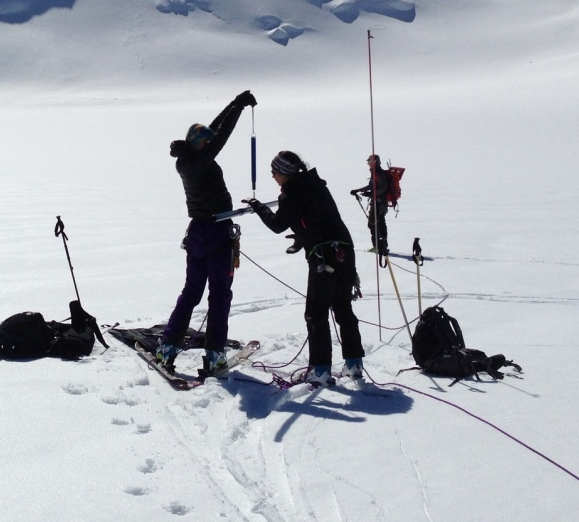
\includegraphics[width=\textwidth]{photo_swe2.jpg}}
        \caption{Weighing the Federal Sampler using the spring scale (units of cm SWE). Photo credit: G. Flowers}
        \label{photo_swe2}
    \end{subfigure}

    \caption{Using the Federal Sampler to measure snow water equivalent}
    \label{photo_swe}
\end{figure}
 
A metric Federal Snow Sampler from Geo Scientific Ltd. was used to measure snow depth and snow water equivalent (SWE). At the predetermined locations, three measurements (within 50\,cm of each other) were made using the sampler. At the snow-pit locations, a total of eight measurements were made, with two measurements on each side of the snow pit. Density calculated from these values will be compared with density determined from sampling within the snow pit (see Section \ref{sec:snowpit}). 

The Federal Snow Sampler consists of four 0.83 m sections that could be screwed together. One end of the sampler has cutter teeth and the other end has a removable thread protector that can be screwed onto the top section of the tube. The sampler has graduations in units of 1\,cm and slits along the side of the tube to allow the observer to determine the length of the core when it is in the tube. The spring scale that comes with the Federal Sampler is in units of cm SWE. To avoid heating the tube, the Federal Sampler is always handled while wearing gloves.

To take a measurement with the Federal Sampler the following steps were taken:
\begin{enumerate}
\item Three depth measurements (within $\sim$50\,cm of each other) were made using an avalanche probe and the depths were recorded.
\item The weight (in cm SWE) of the assembled empty tube was measured using the spring scale and then recorded (tare).
\item The tube was placed vertically into the snow and then pushed and twisted clockwise so that the cutters at the end of the tube would penetrate the snow pack. If this proved to be too difficult, the T-handle was added onto the tube to aid in pushing the tube further into the snow. 
\item When the bottom of the snow pack was reached, the observer would measure the snow depth by using the graduation on the outside of the tube.
\item The tube was then gently pulled out of the snow (so as not to lose any snow from the bottom). The length of the snow core inside the tube was then measured by using the side slits to see the top of the core and reading the height with the graduation on the outside of the tube. This value was then recorded. If the length of the snow core was less than $<$70\% of the snow depth (typically a result of lost snow), the sample measurement was redone.
\item The snow-filled tube was then weighed using the spring scale and the value was recorded.
\item The tube was then emptied and wiped using a soft cloth on a pole to remove any moisture. 
\end{enumerate}

When the T-handle was used, the tube segments often became difficult to take apart. The small handles provided in the kit aided in disassembling the Federal Sampler. However, if a significant force were applied to the T-handle during sampling and the tube segments seized then longer handles (accomplished by attaching snow shovel handles to provided tools) helped in disassembling the sampler. Anti-seizing compound was included in the kit and was applied when needed. A summary of information about completed Federal Sampler measurements can be seen in Table \ref{tab:SWEsummary}.

\subsection{Firn Corer}

The firn corer was intended to be used in the accumulation area to extract a snow/firn core. The coring device would be beneficial in the accumulation area because the core can be extracted and used to determine the location of the snow/firn transition. The snow depth and the mass of the snow core, which included only the past year of snow accumulation, could then be determined. The Federal Sampler was thought to be ineffective in the accumulation area because the snow/firn transition may not have been felt and the core cannot be examined to establish where the transition occurs.

When the corer was used in the field however, a number of problems were encountered that prevented the collection of accurate measurements. The first was that the snow core would get stuck inside the core barrel. Warm temperatures meant that the barrel would get wet from snow melt and when it was inserted into the snow pack, the snow would freeze onto the side of the barrel. As a result, the core was destroyed in the extraction process. The second problem (which was related to the first problem) was that the coring chips in the hole could not be discriminated from the core itself. Coring chips are loose snow crystals that fall to the bottom of the drilling hole when the barrel is taken out. When the barrel is reinserted for the second (or third) core, the snow in the subsequent core will contain these coring chips, which are not part of the intended core. The mass of the core will be overestimated because of this additional snow. This problem is typically avoided by extracting the in-tact core and identifying and removing the coring chips. However, since the core could not be extracted as one piece, this step was not possible. 

In a few locations, sections of the core could be extracted without breaking them apart. In these areas the snow/firn transition could be identified. This means that the firn corer could be used to determine the depth of this transition. The main challenge is therefore being able to identify chips. In firn core trials that occurred after this field work, it was found that the the cores could be pulled out easily if the barrel was not full. However, in these less compacted cores the chips remained difficult to identify so problems persisted. 

As a result of these complications, many planned accumulation area measurements on Glacier 4 and Glacier 2 were abandoned. On Glacier 13, the Federal Sampler was successfully used to obtain snow density measurements. The snow/firn transition could be detected with the Federal Sampler because of a large density change between the snow and firn. In many of these locations, we also dug down to the interface to confirm the snow/firn transition.

\subsection{Snow pit}
\label{sec:snowpit}

\begin{figure}[H]
	\centering
	\fbox{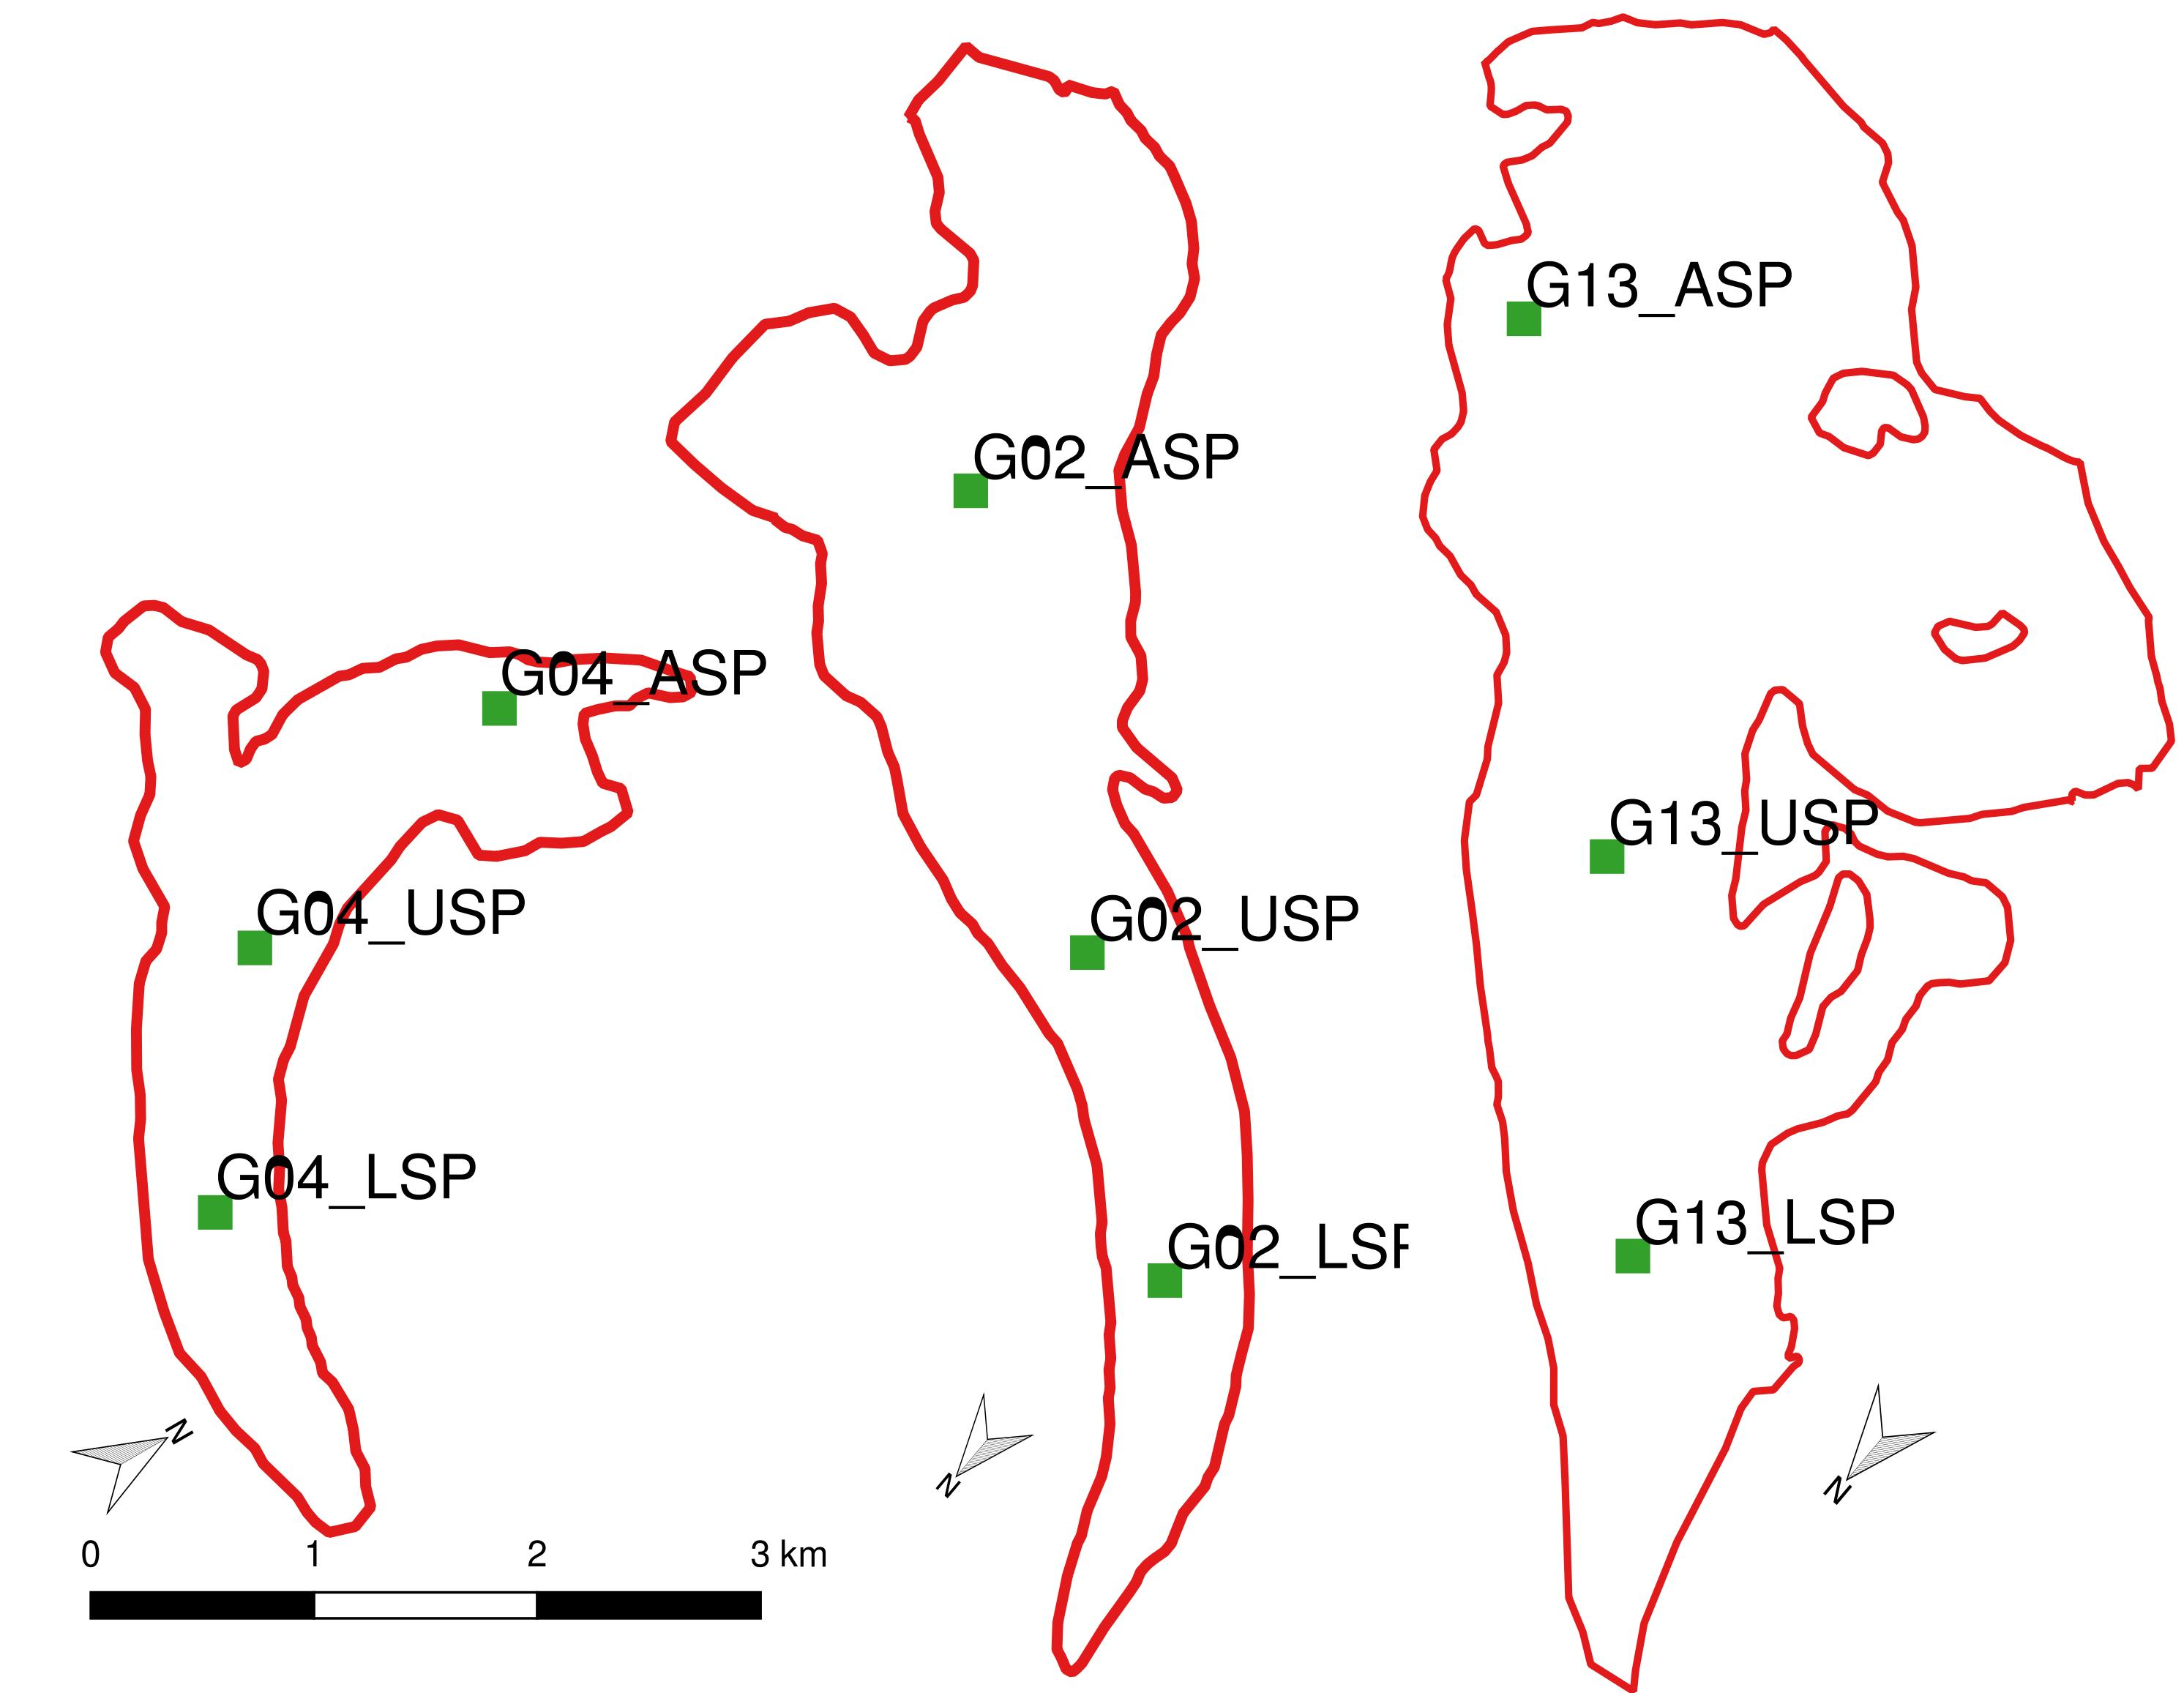
\includegraphics[width = 0.55\textwidth]{map_snowpitlocation_all.jpeg}}\\
	\caption{Locations and labels for all snow pits dug on Glaciers 4, 2 and 13 (left to right).}
	\label{fig:snowpit_location_all}
	\end{figure}

Three snow pits were excavated on each glacier (Figure \ref{fig:snowpit_location_all}) and snow density sampled every 5--10\,cm using a wedge cutter (Snow Metrics RIP 2 Cutter (250 cc)). The snow temperature was also measured at 10\,cm intervals. The snow pit was oriented so that the sampling face was in the shade (typically south wall of snow pit), which reduces melt and radiation-driven changes in temperature of the surface. 

The measurement procedure in the snow pit was as follows:
\begin{enumerate}
\item The face of the wall that was chosen for sampling was smoothed and a ruler was placed against the wall with the 0\,cm mark at the bottom of the snow pit. The ruler was used to measure sampling heights within the snow pack. The snow surface directly above this wall was undisturbed during the digging process so that the true snow depth could be determined. 
\item Air and snow surface temperature were measured by placing the thermometer (dial-stem thermometer ($\pm$0.5$^\circ$)) in the shade of a shovel or ski. 
\item Snow density samples were taken in 10\,cm (or 5\,cm if the snow pack was low) intervals through the full depth of the snow pack. Samples were offset horizontally from each other so that the snow was not affected by previous measurements. 
	\begin{enumerate}
	\item The wedge cutter was inserted into the snow vertically (to sample 10\,cm intervals) and the top was slid onto the wedge to isolate the sample. The wedge was taken out and inspected. If the sample appeared to fill the entire wedge (no obvious voids) then the wedge was emptied into a small plastic bag. If the sample was poor then the snow was discarded and a new sample was taken at the same height in the snow pit. 
	\item A spring scale ($\pm$2.5\,g) was then used to weigh the bag with the snow sample and the weight was recorded. The snow sample was then discarded. Note that the spring scale was tared with an empty bag.
	\end{enumerate}
\item Snow temperatures were also measured and recorded every 10\,cm. The thermometer was inserted into the snow at the desired location and left to equilibrate for several minutes. The temperature was then recorded.
\end{enumerate}

Modifications to this procedure occurred when snow samples could not be taken because the snow was too dense. This would often occur when ice layers or lenses were present in the snow, which could not be cut by the wedge. In these cases, the measured thickness was recorded. A sample would then be taken using the wedge cutter but aligned horizontally so that a 5\,cm tall sample was taken. The sample interval closest to the ice surface (0--10\,cm) would be difficult to obtain because the ice was rough and the snow above was faceted. Sometimes, this sample could not be obtained or a 5\,cm sample needed to be taken. 

After the majority of snow pit measurements were completed, a spring scale with finer resolution was found. For Glacier 4 and 2 the coarse resolution (10\,g) scale had been used but for Glacier 13 the fine resolution (2\,g) scale was used. Future measurements should use the finer resolution spring scale when using the small wedge sampler. As a result, the snow-density uncertainty is larger for Glacier 4 and 2 than for Glacier 13. 

\begin{figure}[H]
	\centering
	\fbox{\includegraphics[width = 0.95\textwidth]{photo_snowpit.jpg}}\\
	\caption{Taking snow denisty measurements in a snow pit. An expandable ruler is used to measure snow depth and determine sampling locations. A 250 cc wedge cutter is used to extract a known volume of snow and a spring scale is used to weigh the snow. The dial-stem thermometer is used for measureing snow temperature. Note that the sampling wall is shaded, has an undistrubed snow surface above it and has a smoothed face. Photo credit: A. Criscitiello}
	\label{photo_snowpit}
	\end{figure}

%%%%
\section{Data processing}
%%%%
\subsection{Snow depth measured with graduated avalanche probe}

\subsubsection{Linear and curvilinear transect surveys}

Snow-depth measurements along the linear and curvilinear transects were taken at locations a certain distance from marked waypoints. Since only the coordinates of the waypoints (WP) were recorded, the coordinates of the measurement locations need to be estimated. The measurement locations were assumed to be 10, 20 and 30 m behind the marked WP, in a straight line between the marked WP and the previous WP (Figure \ref{fig:transect_measure_loc}). In cases with only two observers, locations were assumed to be 10 and 20 m behind the marked WP. For the first marked WP of a transect, it was assumed that the measurement locations were along the same line as that between the first and second WPs. Details of the methodology used to estimate measurement locations can be found in Appendix \ref{app:DataProcessingScripts}.

\begin{figure}[H]
	\centering
	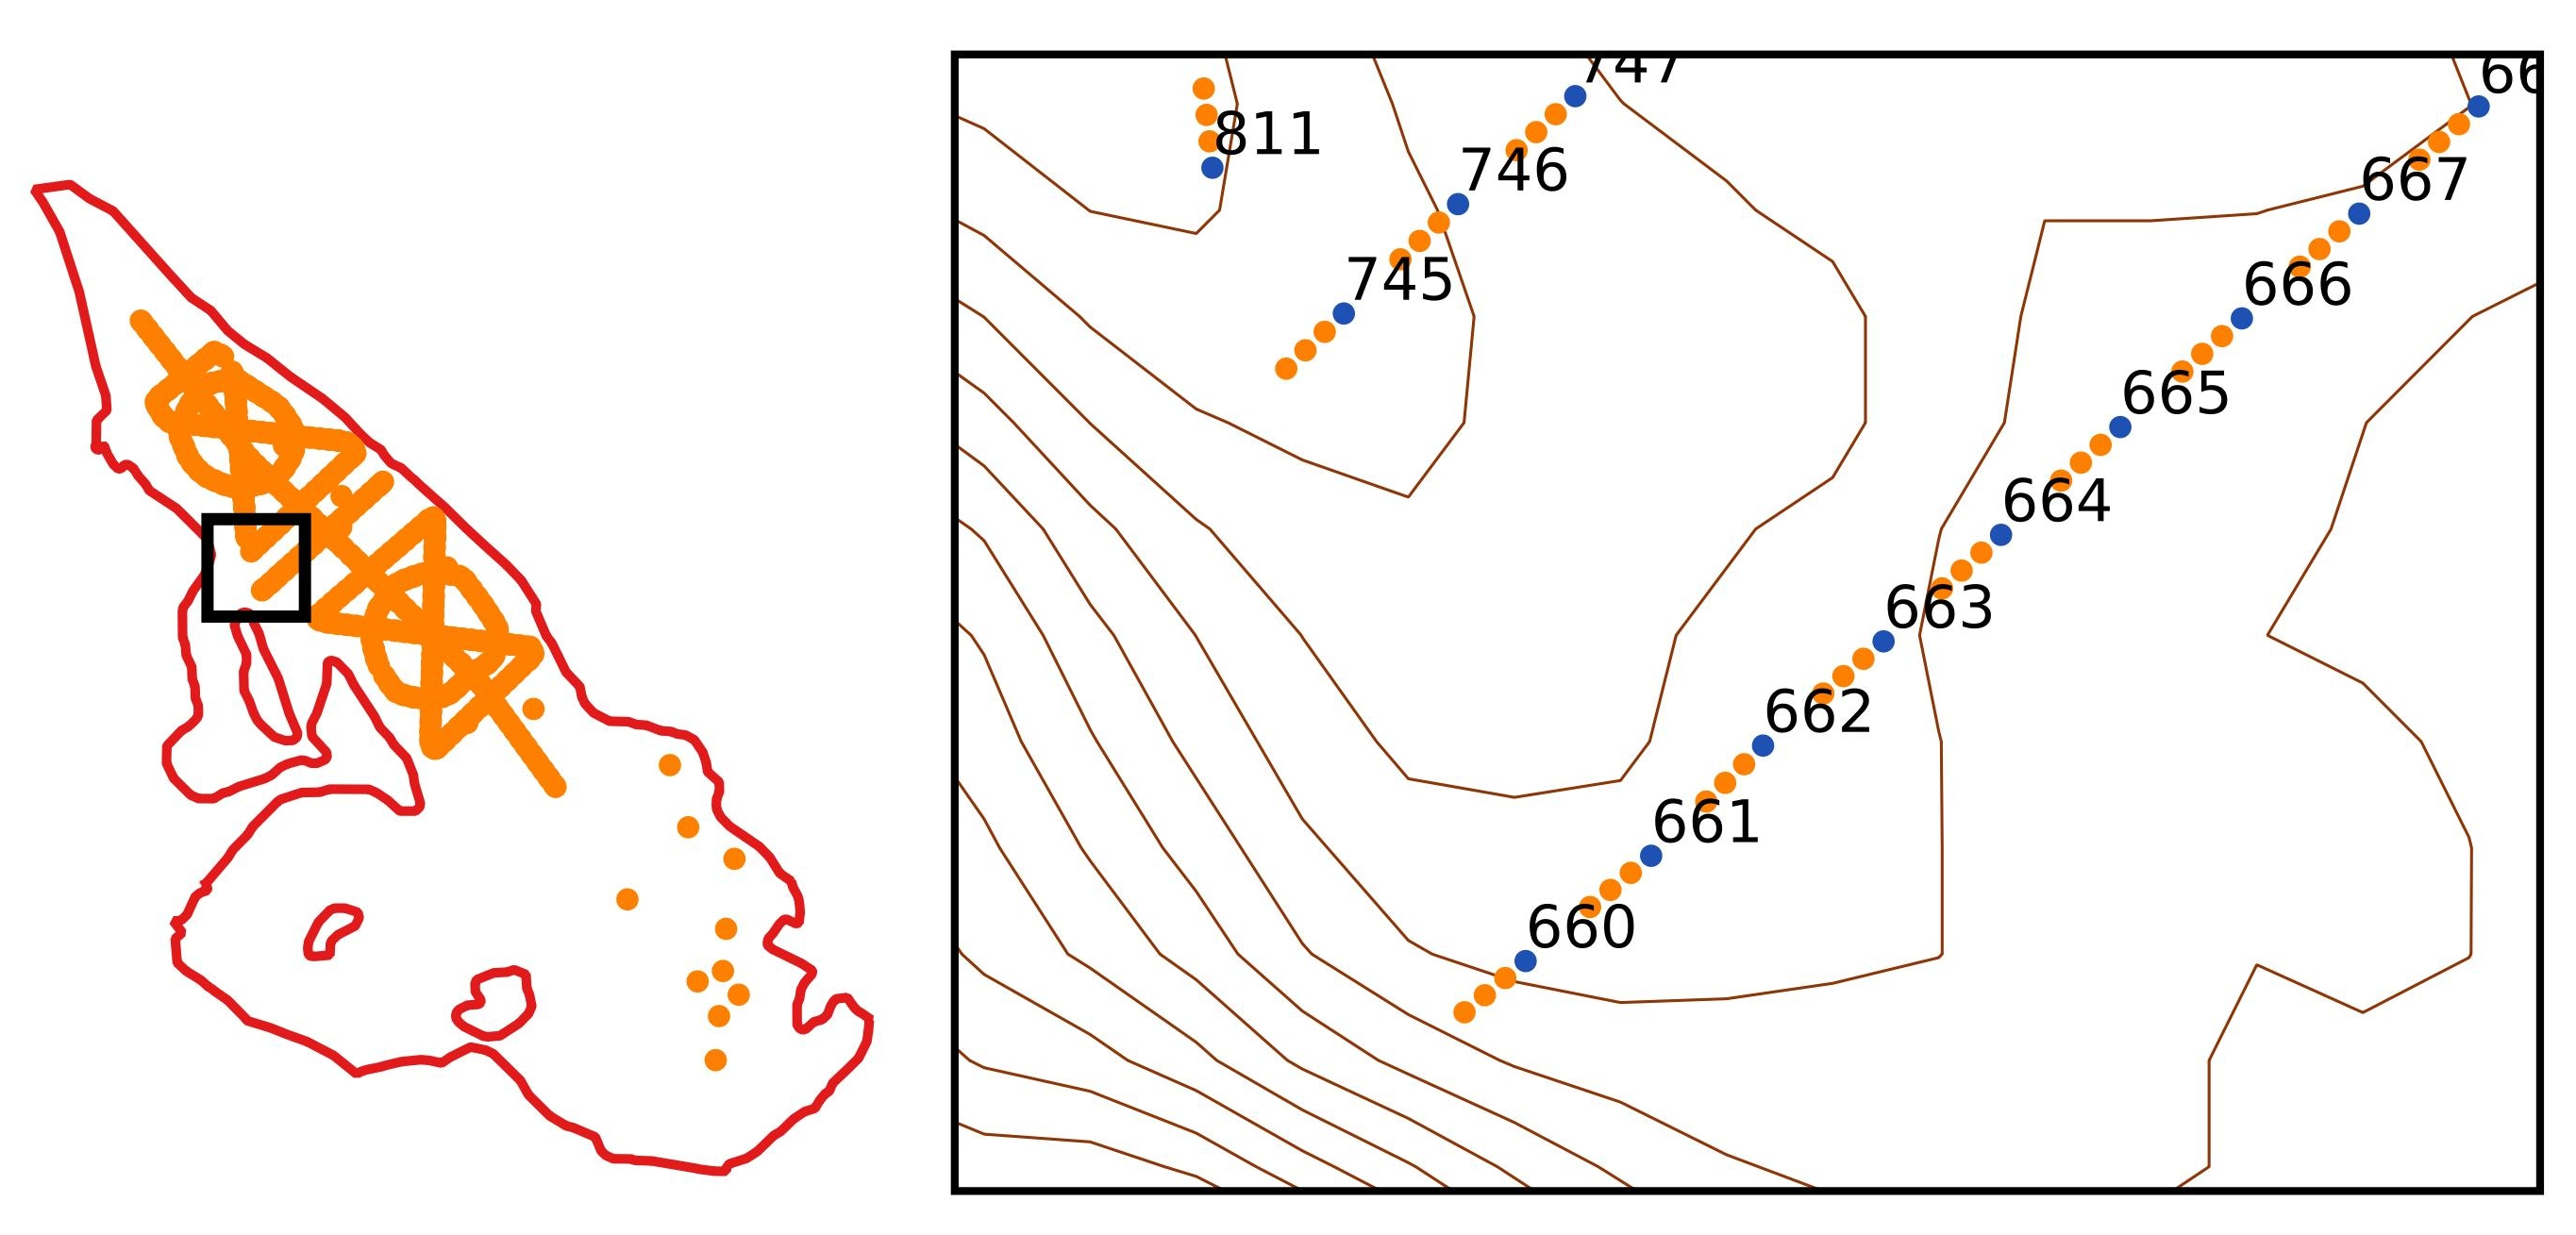
\includegraphics[width = 0.8\textwidth]{transect_measure_locations.jpeg}\\
	\caption{Example of estimating snow depth measurement locations in one area (indicted by black box) on Glacier 13. Numbered waypoint (WP) locations are shown in blue and estimated measurement locations are shown in orange at a distance of 10, 20 and 30 m from the WP. Measurement locations are taken to be along a straight line between subsequent WPs. For the first WP of a transect, the measurement locations are assumed to be along the same line as that between the first and second WPs of a transect. For example, the measurement locations behind WP 660 fall along the same line as those between WP 660 and WP 661. The same is true for WP 745. }
	\label{fig:transect_measure_loc}
\end{figure}

\subsubsection{Zigzag surveys}

\begin{wrapfigure}[25]{R}{0.5\textwidth}
	\centering
	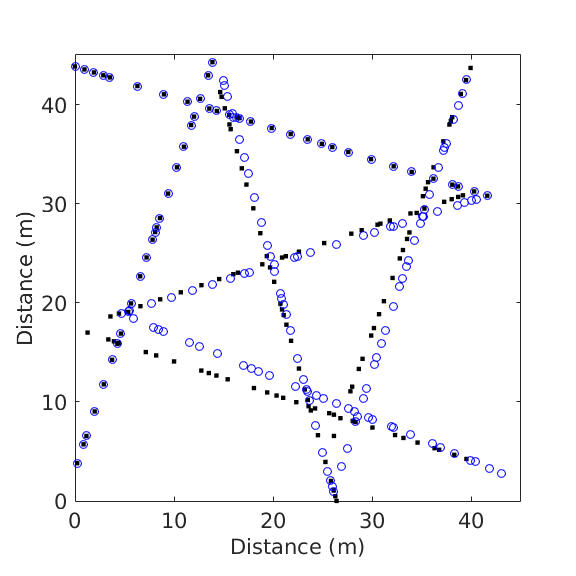
\includegraphics[width = 0.5\textwidth]{Zigzag_calOptions.png}\\
	\caption{Example of zigzag survey measurement locations calculated using different reference vertices for each section of the zigzag. Black squares show measurement locations calculated using the original GPS coordinates of vertices (Option 1). Blue circles show measurement locations calculated using the last measurement location from the previous section as the reference vertex (Option 2). For the first and fifth vertices (located at (0, 40 m) and (0, 4 m)) the original GPS coordinates were used for both options. }
	\label{fig:zigzag_location_options}
\end{wrapfigure}

Depth measurements in zigzag surveys were taken along six sections that connected eight vertices. GPS coordinates of vertices were predetermined. The survey involved navigating to the first vertex, then taking measurements at random distances from this vertex along a straight line between that vertex and the next one. The location of each measurement was measured, using the avalanche probe as a ruler and recorded as the distance from the previous measurement location. Each section was recorded separately and identified by its startingh vertex. 

Originally, the location of measurements was found by taking the cumulative distance of a measurement from its reference vertex along a straight line between the reference and the next vertices. However, it was found that the cumulative distance (measured using an avalanche probe) of each zigzag section was not equivalent to the distance between UTM coordinates of each vertex (due to error in GPS and/or walking between vertices not along a straight line). Therefore, a second option for calculating the measurement locations was established. This second option still assumes the measurement was along a straight line between two vertices but the location is relative to the end of the previous section, not the reference vertex. Vertices 1 and 5 were used as reference vertices for their respective section because they began a section with no prior measurements. An example of differences between these two location estimation methods can be seen in Figure \ref{fig:zigzag_location_options}.


\subsection{Snow density}
\label{sec:snow_density_methods}

The snow pit and Federal Sampler measurements were entered into a spreadsheet and the snow density from each measurement was calculated. For snow-pit measurements the snow density was calculated by multiplying the measured density from each wedge sample by the thickness of the sample and summing these values. This is known as an integrated snow density. A density of 917\,kg\,m$^{-3}$ was applied to ice layers and a density of 600\,kg\,m$^{-3}$ was applied to layers that were described as `hard' and were too difficult to sample. To determine the error in estimating integrated snow density, the values of ice density, ice-layer thickness and the `hard' layer density were varied between 700 and 917\,kg\,m$^{-3}$, $\pm$ 1\,cm (representing 20-100\% of the ice-layer thickness) and 500 and 600\,kg\,m$^{-3}$, respectively.  A summary of density values and ranges is shown in Table \ref{tab:density_stats}.

\begin{table}[b!]
\centering
\caption{Statistics of integrated densities measured using Federal Sampler or vertical density profiles (of snow-wedge measurements) in snow pits. Mean, standard deviation (std) and number ($n$) of snow density measurements on study glaciers is shown.}
\label{tab:density_stats}
\begin{tabular}{c|ccc|ccc}
\multirow{2}{*}{} & \multicolumn{3}{c}{\textbf{Snow pits }} & \multicolumn{3}{| c}{\textbf{Federal Sampler}} \\
 & \begin{tabular}[t]{@{}c@{}}Mean \\ (kg\,m$^{-3}$)\end{tabular} & \begin{tabular}[t]{@{}c@{}}Std \\ (kg\,m$^{-3}$)\end{tabular} & $n$ & \begin{tabular}[t]{@{}c@{}}Mean \\ (kg\,m$^{-3}$)\end{tabular}& \begin{tabular}[t]{@{}c@{}}Std \\ (kg\,m$^{-3}$)\end{tabular}& $n$ \\ \hline \hline
\textbf{Glacier 4} & 348 & 13 & 3 & 327 & 32 & 7 \\
\textbf{Glacier 2} & 333 & 26 & 4 & 326 & 23 & 7 \\
\textbf{Glacier 13} & 349 & 26 & 10 & 307 & 32 & 31 \\ \hline
\textbf{All} & 342 & 26 & 10 & 316 & 31 & 31
\end{tabular}
\end{table}

Density values determined from Federal Sampler measurements that were deemed to be unrepresentative of the local snow pack, including measurements where the inner core length was less than 70\% of the snow depth or where density values were exceptionally high (e.g. 490\,kg\,m$^{-3}$), were removed. The remaining Federal Sampler density values were then averaged for each measurement location.

\subsection{Estimating point-scale winter balance}
\label{sec:swe_calc}

The conversion of measured snow depth to point-scale winter balance cannot not be done at all measurement locations because snow density is not measured at all locations where snow depth is measured. This means that the density measurements need to be interpolated. A subset of appropriate interpolation methods is chosen for this task. In the absence of a clear justification for choosing one option over the other, all options are carried forward in the analysis. 

Four main interpolation methods are used \citep{McGrath2015, Elder1991}. The first assumes a uniform spatial distribution of density, calculated as the mean from all measurement locations on all three glaciers, over the entire study area. The second  also assumes a uniform spatial distribution of density but uses a mean density for individual glaciers (different value for each glacier). The third and fourth methods involve spatially variable density values. One of these methods uses a regression of density on elevation to interpolate between measurement locations. The other spatially variable interpolation method uses an inverse-distance weighted mean for interpolation. 

Since the snow-pit-derived densities and Federal-Sampler-derived densities had no discernible relationship, the two density datasets are kept separate. This means that for each density interpolation option, there are two outputs. In the end, there are eight different interpolations of density that are carried forward throughout the study, allowing for a range of winter balance estimates to be made. 

The eight density distributions can be classified by snow-pit-derived densities (SP) or Federal-Sampler-derived densities (FS) and by the density interpolation method, which is indicated by a number (Table \ref{tab:densityOptions}).
\begin{itemize}
	\item[S1] Calculates the mean density of all snow pit measurements.
	\item[F1] Calculates the mean density of all Federal Sampler measurements.
	\item[S2] Calculates the mean density for each glacier using the snow pit measurements. 
	\item[F2] Calculates the mean density for each glacier using the Federal Sampler measurements. 
	\item[S3] Calculates the slope and intercept of the best-fit regression line of snow-pit densities with elevation for each glacier using the Matlab \texttt{fit} function and then uses slope and intercept to determine density for all elevations associated with each measurement location.
	\item[F3] Calculates the slope and intercept of the best-fit regression line of Federal-Sampler densities with elevation for each glacier using the Matlab \texttt{fit} function and then uses the slope and intercept to determine density for all elevations associated with each measurement location.
	\item[S4] Determines the distance between each depth measurement location and all snow pits and then calculates the inverse-distance weight. For each depth measurement location, each snow pit density is then multiplied by its weight and these values are added together and divided by the sum of all weights. 
	\item[F4] Determines the distance between each depth measurement location and all Federal Sampler measurement locations and then calculates the inverse-distance weight. For each depth measurement location, each Federal Sampler density is then multiplied by its weight and these values are added together and divided by the sum of all weights. 
	\end{itemize}

\begin{table}
\centering
\caption{Eight methods used to estimate snow density at unmeasured locations. Total number of resulting density values given in parentheses, with $n_T$ the total number of snow-depth measurement locations along transects (Table \ref{tab:glacierstats}).}
\label{tab:densityOptions}
\begin{tabular}{cccc}
\hline
\multirow{2}{*}{\textbf{\begin{tabular}[c]{@{}c@{}}Method \\ code \end{tabular}}} & \multicolumn{2}{c}{\textbf{\begin{tabular}[c]{@{}c@{}}Source of measured \\ snow density\end{tabular}}} & \multirow{2}{*}{\textbf{\begin{tabular}[c]{@{}c@{}}Density assignment \\ method\end{tabular}}} \\
 & \textit{Snow pit} & \textit{\begin{tabular}[c]{@{}c@{}}Federal\\ Sampler\end{tabular}} &  \\ \hline
S1 & $\blacksquare$ &  & \multirow{2}{*}{\begin{tabular}[c]{@{}c@{}}Mean of measurements \\ across all glaciers (1)\end{tabular}} \\
F1 &  & $\blacksquare$ &  \\ \hline
S2 & $\blacksquare$ &  & \multirow{2}{*}{\begin{tabular}[c]{@{}c@{}}Mean of  measurements \\ for each glacier (3)\end{tabular}} \\
F2 &  & $\blacksquare$ &  \\ \hline
S3 & $\blacksquare$ &  & \multirow{2}{*}{\begin{tabular}[c]{@{}c@{}}Regression of density on \\ elevation for a glacier ($n_T$)\end{tabular}} \\
F3 &  & $\blacksquare$ &  \\ \hline
S4 & $\blacksquare$ &  & \multirow{2}{*}{\begin{tabular}[c]{@{}c@{}}Inverse distance weighted\\ mean for a glacier ($n_T$)\end{tabular}} \\
F4 &  & $\blacksquare$ & 
\end{tabular}
\end{table}


\subsection{Estimating gridcell-scale winter balance}

We average one to six (mean of 2.1 measurements) point-scale values of WB within each $40 \times 40$\,m DEM gridcell to obtain the gricell-averaged WB (Figure \ref{fig:NumObsPerCell}). The locations of individual measurements have uncertainty due to the error in the horizontal position given by the GPS unit and the estimation of observer location based on the recorded GPS positions of the navigator. This location uncertainty could result in the incorrect assignment of a point-scale WB to a particular gridcell. However, this source of error is not further investigated because we assume that the uncertainty in gridcell-averaged WB is captured in the zigzag measurements described above. Uncertainty due to having multiple observers was also evaluated. There are no significant differences between snow-depth measurements made by observers along any transect (p$>$0.05), with the exception of the first transect on Glacier 4 (51 measurements) (see Appendix \ref{app:variability_data_multiple_scales} for details). 

\begin{figure}[H]
	\centering
	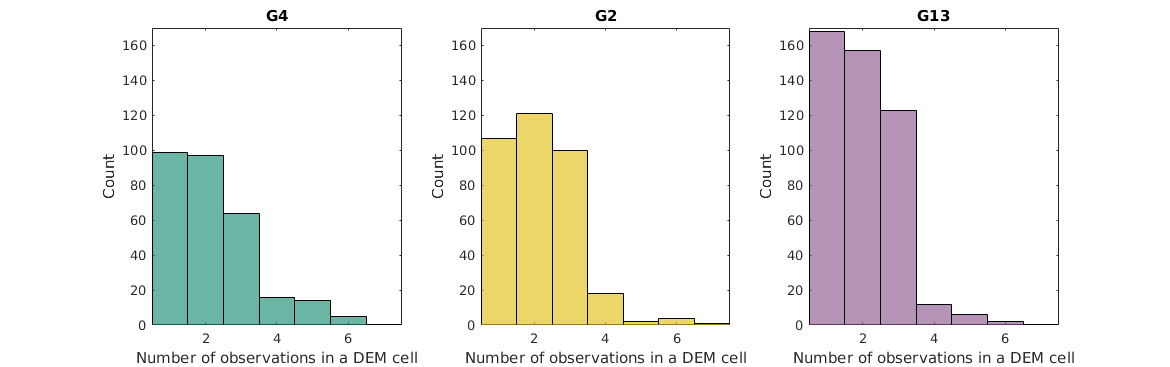
\includegraphics[width =\textwidth]{NumObsPerCell.png}\\
	\caption{Number of measurement locations within DEM gridcells.}
	\label{fig:NumObsPerCell}
\end{figure}


\section{Summary}

Within this chapter, I describe the design and implementation of a snow survey on three glaciers as well as the initial data processing. The experimental design is structured to measure WB at multiple scales. The regional-scale variability is investigated by taking measurements on three glaciers within a mountain range. The basin-scale variability is investigated by taking snow depth measurements along linear and curvilinear transects that cover large areas of the glaciers. The transects include a centreline with multiple transverse transects pattern and an hourglass with inscribed circle. Measurement locations are calculated based on GPS waypoints, assumed distances between observers and known direction of travel. The gridcell-scale variability is investigated by taking many snow depth measurements within a single gridcell in the zigzag survey. At least three zigzags surveys were completed on each glacier. Finally, the point-scale variability is investigated by making at least three snow-depth observations at each measurement location. Snow density is measured at three locations on each glacier using a wedge sampler in a snow pit as well as at 7--17 locations across each glacier using a Federal Sampler. To obtain estimates of point-scale winter balance, point-scale snow depth values are averaged and then multiplied by the assigned density value. Gridcell-scale winter balance values are the obtained by averaging point-scale WB values within a gridcell. 



%%%%%%%%%%%%%%%%%%%%%%%%%%

%%%%%%%%%%%%%%%%%%%%%%%%%
\chapter{Field results}

This chapter presents collected snow density and depth data. Section 3.1 examines snow density and its associated uncertainty, with a focus on understanding discrepancies between the snow-pit-derived and Federal-Sampler-derived densities. The relationship between density and elevation is also examined. Basic statistics are then used to examine snow depth variability at multiple scales. Sections 3.2 and 3.3 summarize snow depth data from the transects and zigzag surveys, respectively. A brief description of point-scale winter balance values is presented in Section 3.4. Appendix \ref{app:DataProcessingScripts} contains a more detailed description of steps used in the data processing.


%%%
\section{Density}
%%%
\label{sec:density}

\subsection{Basic statistics}

Snow pit (SP)-derived regional (S1) and glacier-mean (S2) densities are within one standard deviation of the corresponding Federal Sampler (FS)-derived densities (F1 and F2) although SP-derived density values are larger (Table \ref{tab:density_stats}). For both SP- and FS-derived densities, the mean density for any given glacier (S2 or F2) is within one standard deviation of the mean across all glaciers (S1 or F1). For any given glacier, the standard deviation of the 3--4 SP- or FS-derived densities is $<$13\% of the mean of those values (S2 or F2). Note that the mean of all Federal Sampler derived density values was skewed by the proportionally large number of measurements obtained on Glacier 13.

\subsection{Federal Sampler measurements and snow depth}
\label{sec:FSdensity&depth}

There is a positive linear relationship (R$^2$ = 0.59, p$<$0.01) between measured snow density and depth for all Federal Sampler measurements (Figure \ref{fig:all_depth}). This positive relationship could be a result of physical processes, such as compaction in deep snow and preferential formation of depth hoar in shallow snow, but is more likely a result of measurement artefacts for a number of reasons. First, the range of densities measured by the Federal sampler seems improbably large (225--410\,kg\,m$^{-3}$) given the conditions at the time of sampling. Previous unpublished density measurements taken on Glacier 2 for five study years have a mean snow density of 298\,kg\,m$^{-3}$ and a standard deviation of 48\,kg\,m$^{-3}$ (range of 264-396\,kg\,m$^{-3}$ with a maximum density difference of 110\,kg\,m$^{-3}$ in any one year) (Flowers, 2016, personal communication). Second, compaction effects of the magnitude required to explain the density differences between SP and FS measurements would not be expected at the measured snow depths (up to 340\,cm). Third, no linear relationship exists between depth and SP-derived density (R$^2 =$ 0.05). These findings suggest that the Federal Sampler measurements have a bias for which I have not identified a suitable correction. 

The Federal Sampler appears to oversample in deep snow and undersample in shallow snow. Oversampling by small-diameter (3.2--3.8\,cm) sampling tubes has been observed in previous studies, with a percent error between 6.8\% and 11.8\% \citep[e.g.][]{Work1965, Fames1982, Conger2009}. Studies that use Federal Samplers often apply a 10\% correction to all measurements for this reason \citep[e.g.][]{Molotch2005}. Oversampling has been attributed to slots ``shaving'' snow into the tube as it is rotated \citep[e.g.][]{Dixon2012} and to snow falling into the slots, particularly for snow samples with densities $>$400\,kg\,m$^{-3}$ and snow depths $>$1\,m \citep[e.g.][]{Beaumont1963}. Undersampling is likely to occur due to loss of snow from the bottom of the sampler \citep{Turcan1975}. Loss by this mechanism may have occurred in this study, given the isothermal and melt-affected snow conditions observed over the lower reaches of Glaciers 2 and 13. Relatively poor Federal Sampler spring-scale sensitivity also calls into question the reliability of measurements for snow depths $<$20\,cm.



\begin{figure}[p]
	\centering
	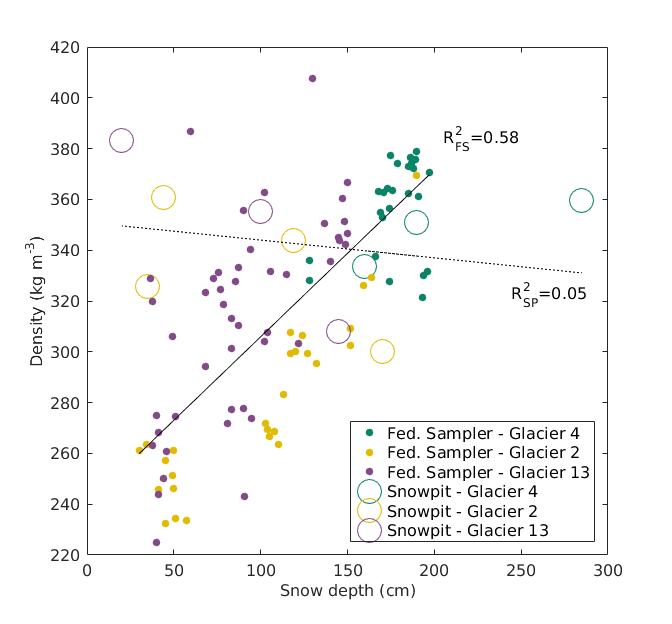
\includegraphics[width =0.85\textwidth]{DepthDensity_SWEonly.png}\\
	\caption{Relationship between measured density and snow depth for all Federal Sampler and snow pit locations. A linear regression of density on depth for Federal Sampler measurements is shown as a solid line and for snow pits is shown as a dashed line.}
	\label{fig:all_depth}
\end{figure}


\subsection{Density uncertainties}

\subsubsection{Snow-pit-derived densities}

Uncertainty in estimating density from snow pits (SP) stems from measurement errors and incorrect assignment of density to layers that could not be sampled (see Section \ref{sec:snow_density_methods}). When accounting for these uncertainties, the range of integrated density values is always less than 15\% of the reference density, with the largest ranges present on Glacier 2 (Table \ref{tab:density_SP}). Depth-averaged densities for shallow pits ($<$50\,cm) that contain ice lenses are particularly sensitive to changes in prescribed density and ice-lens thickness.

\begin{sidewaystable}[]
\centering
\caption{Summary of integrated snow density values calculated from snow-pit measurements. The reference density values are calculated with an ice-layer density of 917\,kg\,m$^{-3}$ and a `hard' snow density of 600\,kg\,m$^{-3}$. To determine the error in estimating integrated snow density, ice density, ice thickness and the `hard' layer density are varied between 700 and 917\,kg\,m$^{-3}$, $\pm$ 1\,cm and 500 and 600\,kg\,m$^{-3}$, respectively.}
\label{tab:density_SP}
\resizebox{\textwidth}{!}{%
\begin{tabular}{lcccccccc}
\multirow{2}{*}{\textbf{Snow pit name}} &  & \multicolumn{4}{c}{\textbf{Density (kg m$^{-3}$)}} &  \\
\multirow{-2}{*}{} & \multirow{-2}{*}{\textbf{Depth (m)}} & \textit{Reference} & \textit{Minimum} & \textit{Maximum} & \textit{Range} & \multirow{-2}{*}{\textbf{\begin{tabular}[c]{@{}c@{}}Range as \% \\ of reference value\end{tabular}}} & \multirow{-2}{*}{\textbf{\begin{tabular}[c]{@{}c@{}}Elevation\\ (m a.s.l)\end{tabular}}}& \multirow{-2}{*}{\textbf{\begin{tabular}[c]{@{}c@{}}Average \\ Temperature ($^{\circ}$) \end{tabular}}}\\ \hline \hline

Glacier 4, Lower & 190 & 350.9 & 343.2 & 359.1 & 15.9 & 4.5 & 2154 & $-$ 4.3\\
Glacier 4, Upper & 160 & 333.4 & 316.6 & 349.6 & 33.0 & 9.9  & 2298 & $-$ 5.7\\
Glacier 4, Accumulation& 285 & 359.7 & 356.6 & 362.4 & 5.8 & 1.6  & 2482 & $-$ 6.8\\  \hline
Glacier 2, Lower  & 44 & 360.9 & 328.6 & 377.3 & 48.7 & 13.5 & 2175 & $-$ 3.7 \\
Glacier 2, Zone 4A & 35 & 325.8 & 307.9 & 344.7 & 36.8 & 11.3 & 2261 & $-$ 3.4 \\
Glacier 2, Upper  & 119 & 344.0 & 327.1 & 361.9 & 34.8 & 10.1 & 2349 & $-$ 6.6 \\ 
Glacier 2, Accumulation & 170 & 300.2 & 298.6 & 303.1 & 4.5 & 1.5  & 2550 & $-$ 7.4\\  \hline
Glacier 13, Lower  & 20 & 383.0 & 383.0 & 383.0 & 0 & 0  & 2139 & $-$ 0.1\\
Glacier 13, Upper & 100 & 355.4 & 345.6 & 366.9 & 21.3 & 6.0 & 2257 & $-$ 1.7 \\
Glacier 13, Accumulation & 145 & 307.8 & 306.4 & 308.2 & 1.8 & 0.6 & 2521 & $-$ 5.6
\end{tabular}%
}
\end{sidewaystable}

\subsubsection{Federal-Sampler-derived densities}

Error in Federal Sampler (FS)-derived densities is calculated as the standard deviation of the 3--8 measurements taken at each sampling location. The mean FS-derived density has a large range of values over the study glaciers (227--431\,kg\,m$^{-3}$) (Table \ref{tab:density_TubeRange}). The FS-derived density range as a percentage is also large ($>$25\%) for many of the measurement locations. 

\begin{table}[]
\centering
\caption{Range of densities estimated from Federal Sampler measurements. The number ($n$) of reliable measurements, as well as the minimum, maximum and mean density are shown. The density range, given as a percent of the mean density, is also shown. Location refers to the snow pit name as shown in Figure \ref{fig:snowpit_location_all}.}
\label{tab:density_TubeRange}
\begin{tabular}{lcccccc}
\multicolumn{1}{c}{\multirow{2}{*}{\textbf{Location}}} & \multirow{2}{*}{\textbf{$n$}} & \multicolumn{3}{c}{\textbf{Density (kg m$^{-3}$)}} & \multirow{2}{*}{\textbf{\begin{tabular}[c]{@{}c@{}}Range as \%\\ of mean (\%)\end{tabular}}}& \multirow{2}{*}{\textbf{\begin{tabular}[c]{@{}c@{}}Elevation\\ (m a.s.l)\end{tabular}}} \\
\multicolumn{1}{c}{} &  & Mean & Minimum & Maximum &  \\ \hline  \hline
G04\_Z3A\_SWE & 3 & 334 & 309 & 358 & 14 & 2229 \\
G04\_USP & 6 & 311 & 274 & 353 & 22 & 2298 \\
G04\_Z2A\_SWE & 3 & 360 & 303 & 431 & 35 & 2162 \\
G04\_LSP & 7 & 272 & 250 & 297 & 13 & 2154 \\
G04\_Z5B\_SWE & 2 & 337 & 324 & 350 & 7  & 2360\\
G04\_Z5A\_SWE & 3 & 311 & 275 & 351 & 21  & 2328\\
G04\_Z5C\_SWE & 2 & 361 & 350 & 373 & 6  & 2332\\  \hline
G02\_Z5C\_SWE & 2 & 296 & 245 & 347 & 28 & 2332 \\
G02\_USP & 7 & 294 & 232 & 353 & 34  & 2349\\
G02\_Z7A\_SWE & 3 & 326 & 304 & 349 & 12  & 2403\\
G02\_Z7B\_SWE & 2 & 336 & 320 & 351 & 9 & 2458 \\
G02\_Z7C\_SWE & 3 & 351 & 338 & 365 & 7 & 2442 \\
G02\_Z3B\_SWE & 3 & 349 & 341 & 353 & 3  & 2172\\
G02\_LSP\_SWE & 7 & 331 & 302 & 349 & 13 & 2175 \\ \hline
G13\_ASP & 8 & 343 & 277 & 395 & 33  & 2521\\
G13\_651 & 3 & 329 & 318 & 345 & 7  & 2574\\
G13\_652 & 2 & 319 & 291 & 346 & 15  & 2542\\
G13\_654 & 3 & 298 & 266 & 318 & 14  & 2571\\
G13\_655 & 1 & 300 &-- & -- & --  & 2561\\
G13\_656 & 3 & 279 & 227 & 315 & 24  & 2541\\
G13\_657 & 3 & 331 & 323 & 338 & 4  & 2483\\
G13\_658 & 2 & 343 & 333 & 354 & 6  & 2427\\
G13\_659 & 3 & 245 & 232 & 258 & 7 & 2327 \\
G13\_Z7C\_SWE & 2 & 270 & 253 & 287 & 9  & 2297\\
G13\_USP & 6 & 294 & 247 & 359 & 31  & 2258\\
G13\_Z4C\_SWE & 4 & 342 & 334 & 350 & 5 & 2206 \\
G13\_744 & 3 & 323 & 298 & 347 & 14 & 2210 \\
G13\_Z3B\_SWE & 3 & 333 & 308 & 351 & 12 & 2156 \\
G13\_Z4B\_SWE & 2 & 332 & 312 & 351 & 11  & 2214\\
G13\_Z5A\_SWE & 3 & 276 & 240 & 301 & 17  & 2271\\
G13\_Z5B\_SWE & 2 & 255 & 254 & 257 & 1 & 2226
\end{tabular}
\end{table}

\subsection{Comparing density from snow pit and Federal Sampler measurements}

To directly compare SP-derived densities and FS-derived densities, eight FS measurements were taken around two snow-pit locations on each study glacier.  The overall range of FS-derived densities is larger than that of the SP-derived density values (Figure \ref{fig:density_pitVStube}). Within the minimum and maximum SP-derived densities, the values are indistinguishable for all SP locations, except for the snow pit in the accumulation area on Glacier 13 (`G13\_ASP').

\begin{figure}[H]
	\centering
	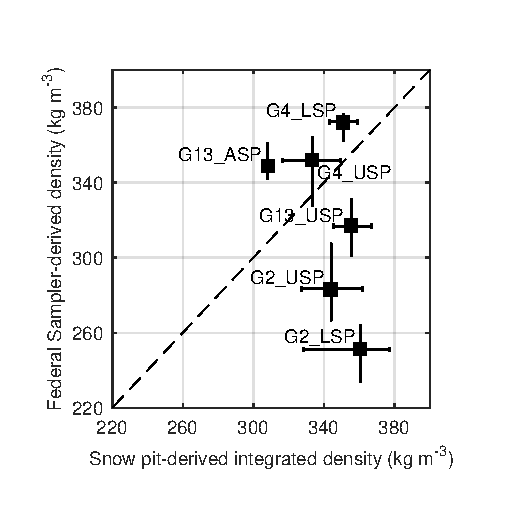
\includegraphics[width =0.7\textwidth]{SPvsFS.pdf}\\
	\caption{Comparison of depth-averaged densities estimated using Federal Sampler (FS) measurements and a wedge cutter in a snow pit (SP)  for Glacier 4 (G4), Glacier 2 (G2) and Glacier 13 (G13). Labels indicate snow pit locations in the accumulation area (ASP), upper ablation area (USP) and lower ablation area (LSP). Error bars for SP-derived densities are calculated by varying the thickness and density of layers that are too hard to sample (Table \ref{tab:density_SP}) and error bars for FS-derived densities are the standard deviation of measurements taken at one location (Table \ref{tab:density_TubeRange}). One-to-one line is dashed.}
	\label{fig:density_pitVStube}
\end{figure}


\subsection{Density and elevation}

A linear regression of density on topographic parameters is often used to interpolate density values between measurement locations \citep[e.g.][]{Elder1998, Molotch2005,Wetlaufer2016}. Since the density measurement locations spanned a large fraction of the elevation range for each glacier, the density values are regressed on elevation only. 

Regression slopes differ in both magnitude and sign for SP-derived and FS-derived densities (Table \ref{tab:elev_regress}). SP-derived density decreases with elevation on Glaciers 2 and 13 and does not change with elevation on Glacier 4 (Figure \ref{fig:elev_snowpit}). The lower elevation sites on Glaciers 2 and 13 could have been melt affected. Warmer mean snow temperatures at the lower sites (Table \ref{tab:density_SP}) indicate that melt has occurred, which would increase snow density. Glacier 4 was probably not affect by melt, as snow temperatures were low at all SP sites. 

Opposite relationships are seen in the regression of FS-derived densities on elevation (Figure \ref{fig:elev_tube}). Density increases with elevation on Glacier 2 and there is no relationship with elevation on Glacier 4 and 13. The positive relationship between FS-derived density and elevation on Glacier 2 is likely enhanced because of the combination of a positive relationship between FS-derived density and snow depth (Section \ref{sec:FSdensity&depth}) and a positive relationship between snow depth and elevation on Glacier 2 (Figure \ref{fig:depth_elev}). Since there is no significant relationship between snow depth and elevation on Glaciers 4 and 13, the relationship between snow density and elevation is weak. 


\begin{table}[]
\centering
\caption{Summary of linear regressions between integrated density and elevation (m a.s.l.). }
\label{tab:elev_regress}
\begin{tabular}{lrrcrcc}
\multicolumn{1}{c}{\multirow{2}{*}{\textbf{Location}}} & \multicolumn{3}{c}{\textbf{\begin{tabular}[c]{@{}c@{}}Snow pit \\ Regression\end{tabular}}} & \multicolumn{3}{c}{\textbf{\begin{tabular}[c]{@{}c@{}}Fed. Sampler\\ Regression\end{tabular}}} \\
\multicolumn{1}{c}{} & \multicolumn{1}{c}{Equation} & \multicolumn{1}{c}{R$^2$} & \multicolumn{1}{l}{$n$} & \multicolumn{1}{c}{Equation} & R$^2$ & \multicolumn{1}{l}{$n$} \\ \hline \hline
Glacier 4 & 0.03$z+$274 & 0.16 & 3 & $-$0.16$z+$714 & 0.53 & 7 \\
Glacier 2 & $-$0.14$z+$659 & 0.75 & 4 & 0.24$z-$282 & 0.72 & 7 \\
Glacier 13 & $-$0.20$z+$802 & $>$0.99 & 3 & 0.12$z+$33 & 0.21 & 17 \\ \hline
All & $-$0.12$z+$618 & 0.50 & 10 & $-$0.14$z+$659 & 0.75 & 31
\end{tabular}
\end{table}


\begin{figure}[H]
  \makebox[\textwidth][c]{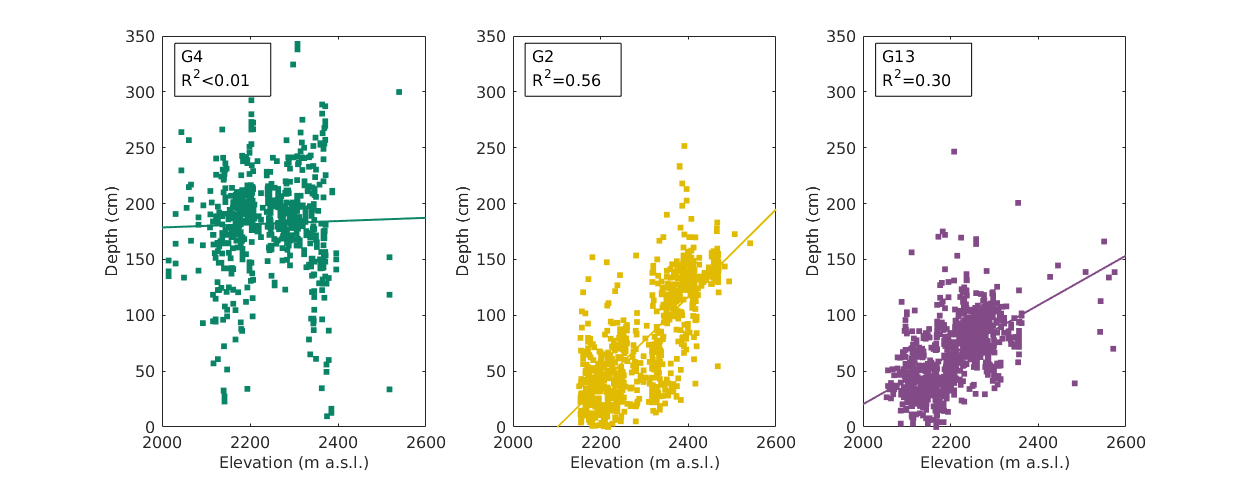
\includegraphics[width=1.2\textwidth]{DepthElevation.png}}%
	\caption{Relationship between measured snow depth and elevation at all sampling locations for Glaciers 4 (G04), 2 (G02) and 13 (G13).}
	\label{fig:depth_elev}
\end{figure}


\begin{figure}[H]
	\centering
	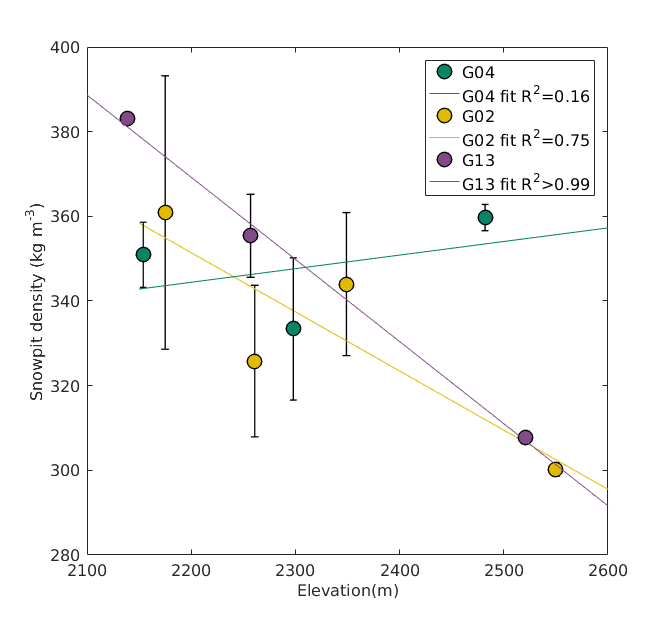
\includegraphics[width = 0.5\textwidth]{ElevationVsSnowpit_all.png}\\
	\caption{Relationship between snow-pit-derived density and elevation for Glaciers 4 (G04), 2 (G02) and 13 (G13).}
	\label{fig:elev_snowpit}
\end{figure}


\begin{figure}[H]
	\centering
	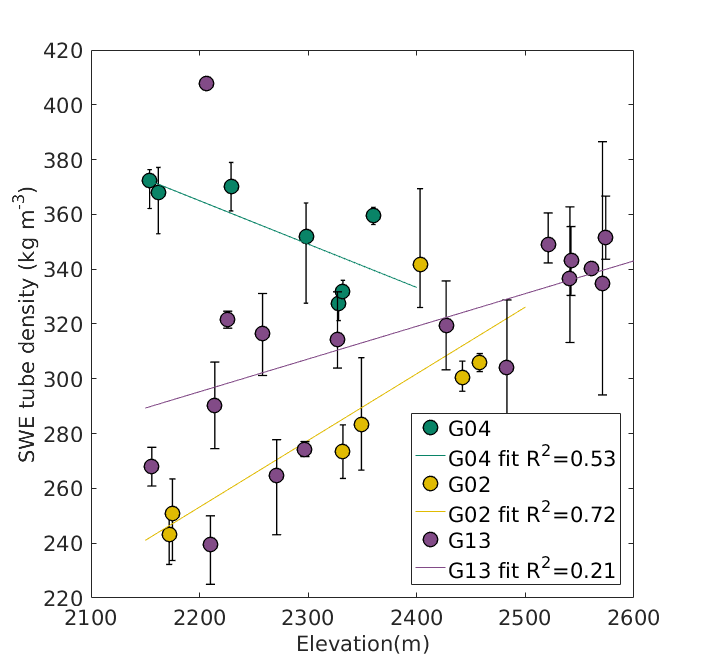
\includegraphics[width = 0.5\textwidth]{ElevationVsSWEtube_all.png}\\
	\caption{Relationship between Federal-Sampler-derived density and elevation for Glaciers 4 (G04), 2 (G02) and 13 (G13).}
	\label{fig:elev_tube}
\end{figure}


%%%%%%%%%%%%%%%%%%%%%%%%%%%%%%%%%%%%%%
\section{Linear and curvilinear transect snow depth data}

\begin{figure}[H]
    \centering
    \begin{subfigure}[b]{0.48\textwidth}
        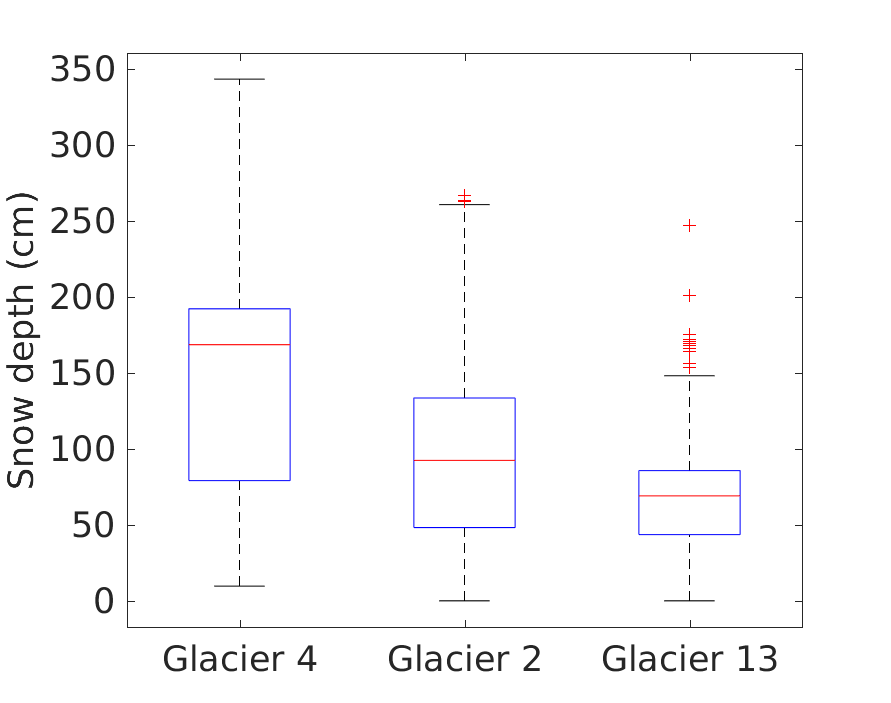
\includegraphics[width=\textwidth]{box_depth_wZZ.png}
        \caption{ }
        \label{fig:box_depth_wZZ}
    \end{subfigure}
    ~
    \begin{subfigure}[b]{0.48\textwidth}
        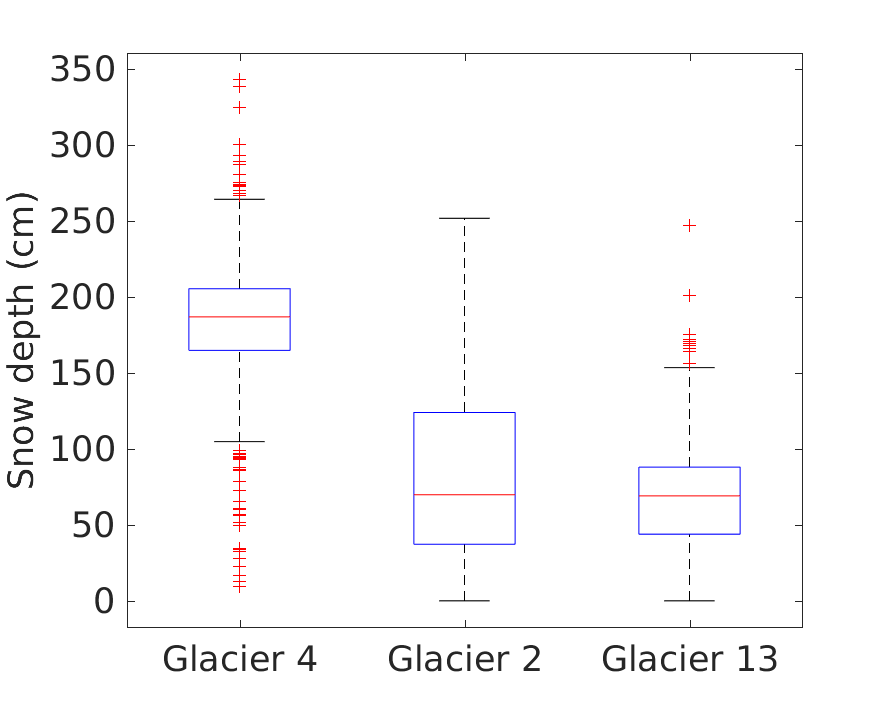
\includegraphics[width=\textwidth]{box_depth_noZZ.png}
        \caption{}
        \label{fig:box_depth_noZZ}
    \end{subfigure}

    \caption{Boxplots of snow depth measured on study glaciers. (a) All snow depth values. (b) Snow depth values only from transects (zigzag, snow pit and Federal Sampler measurements excluded). Red line indicates median, blue box shows first quantiles, bars indicate minimum and maximum values (excluding outliers) and red crosses show outliers, which are defined as being outside of the range of 1.5 times the quartiles (approximately $\pm2.7\sigma$).}
    \label{fig:box_depth_transects}
\end{figure}

Glacier 4 has the largest median and range of snow depth values, while Glacier 13 has the smallest (Figure \ref{fig:box_depth_transects}). The boxplot of snow depth on Glacier 4 has different characteristics when only transect data is plotted (zigzag, snow pit and Federal Sampler measurements excluded). The range and IQR are smaller and there are significantly more points that are considered outliers. 

%%%%%%%%%%%%%%%%%%%%%%%%%%%%%%%%%%%%%%
\section{Zigzag snow-depth data}

A comparison of measured snow depth for each zigzag is shown in Figure \ref{fig:ZZ_boxplot}. The snow-depth data from zigzag surveys on Glacier 4 have the smallest range of values observed and few outliers. The mean depth is significantly greater at the highest elevation zigzag. Zigzags on Glacier 2 show more variability. The range of depth values is greatest within the mid-glacier zigzag survey and the upper zigzag survey has many outliers. The zigzags on Glacier 13 do not vary considerably in range, although the lower zigzags show a large number of outliers which may be a result of these locations being close to a supraglacial meltwater channel. 

The depths measured in each zigzag on Glaciers 4, 2 and 13 are shown in Figures \ref{fig:ZZ_G04}, \ref{fig:ZZ_G02} and \ref{fig:ZZ_G13}, respectively. There is considerable variability both between zigzags and within each zigzag. For example, snow depths in G04\_Z5B are more uniform than in G04\_Z3A (Figure \ref{fig:ZZ_G04}). The average standard deviation of all zigzag depth measurements is 0.07\,m, 0.17\,m and 0.14\,m, for Glaciers 4, 2 and 13, respectively. When converted to values of WB using the local FS-derived density measurement, the average standard deviation is 0.027\,m\,w.e., 0.035\,m\,w.e. and 0.040 \,m\,w.e. WB data for each zigzag are not normally distributed.

\begin{figure}[H]
	\centering
	 \makebox[\textwidth][c]{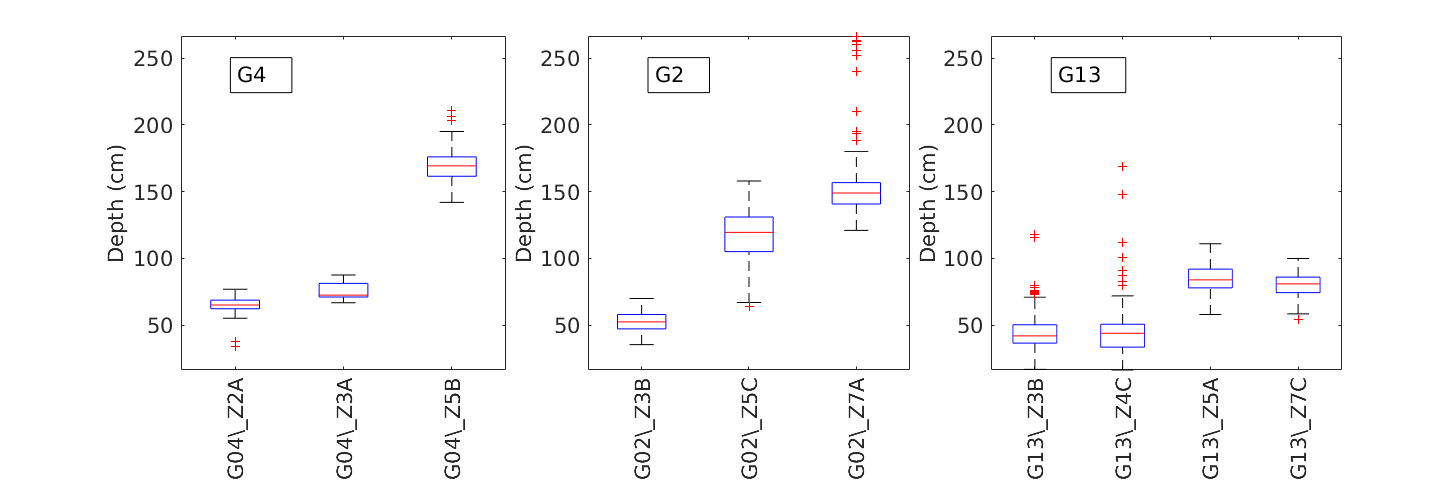
\includegraphics[width = 1.1\textwidth]{Zigzag_Boxplot.png}}%
	\caption{Boxplots of snow depth data measured at each zigzag location. See Figure \ref{fig:ZZ_locations} for locations of each zigzag.}
	\label{fig:ZZ_boxplot}
\end{figure}


\begin{figure}[H]
	\centering
	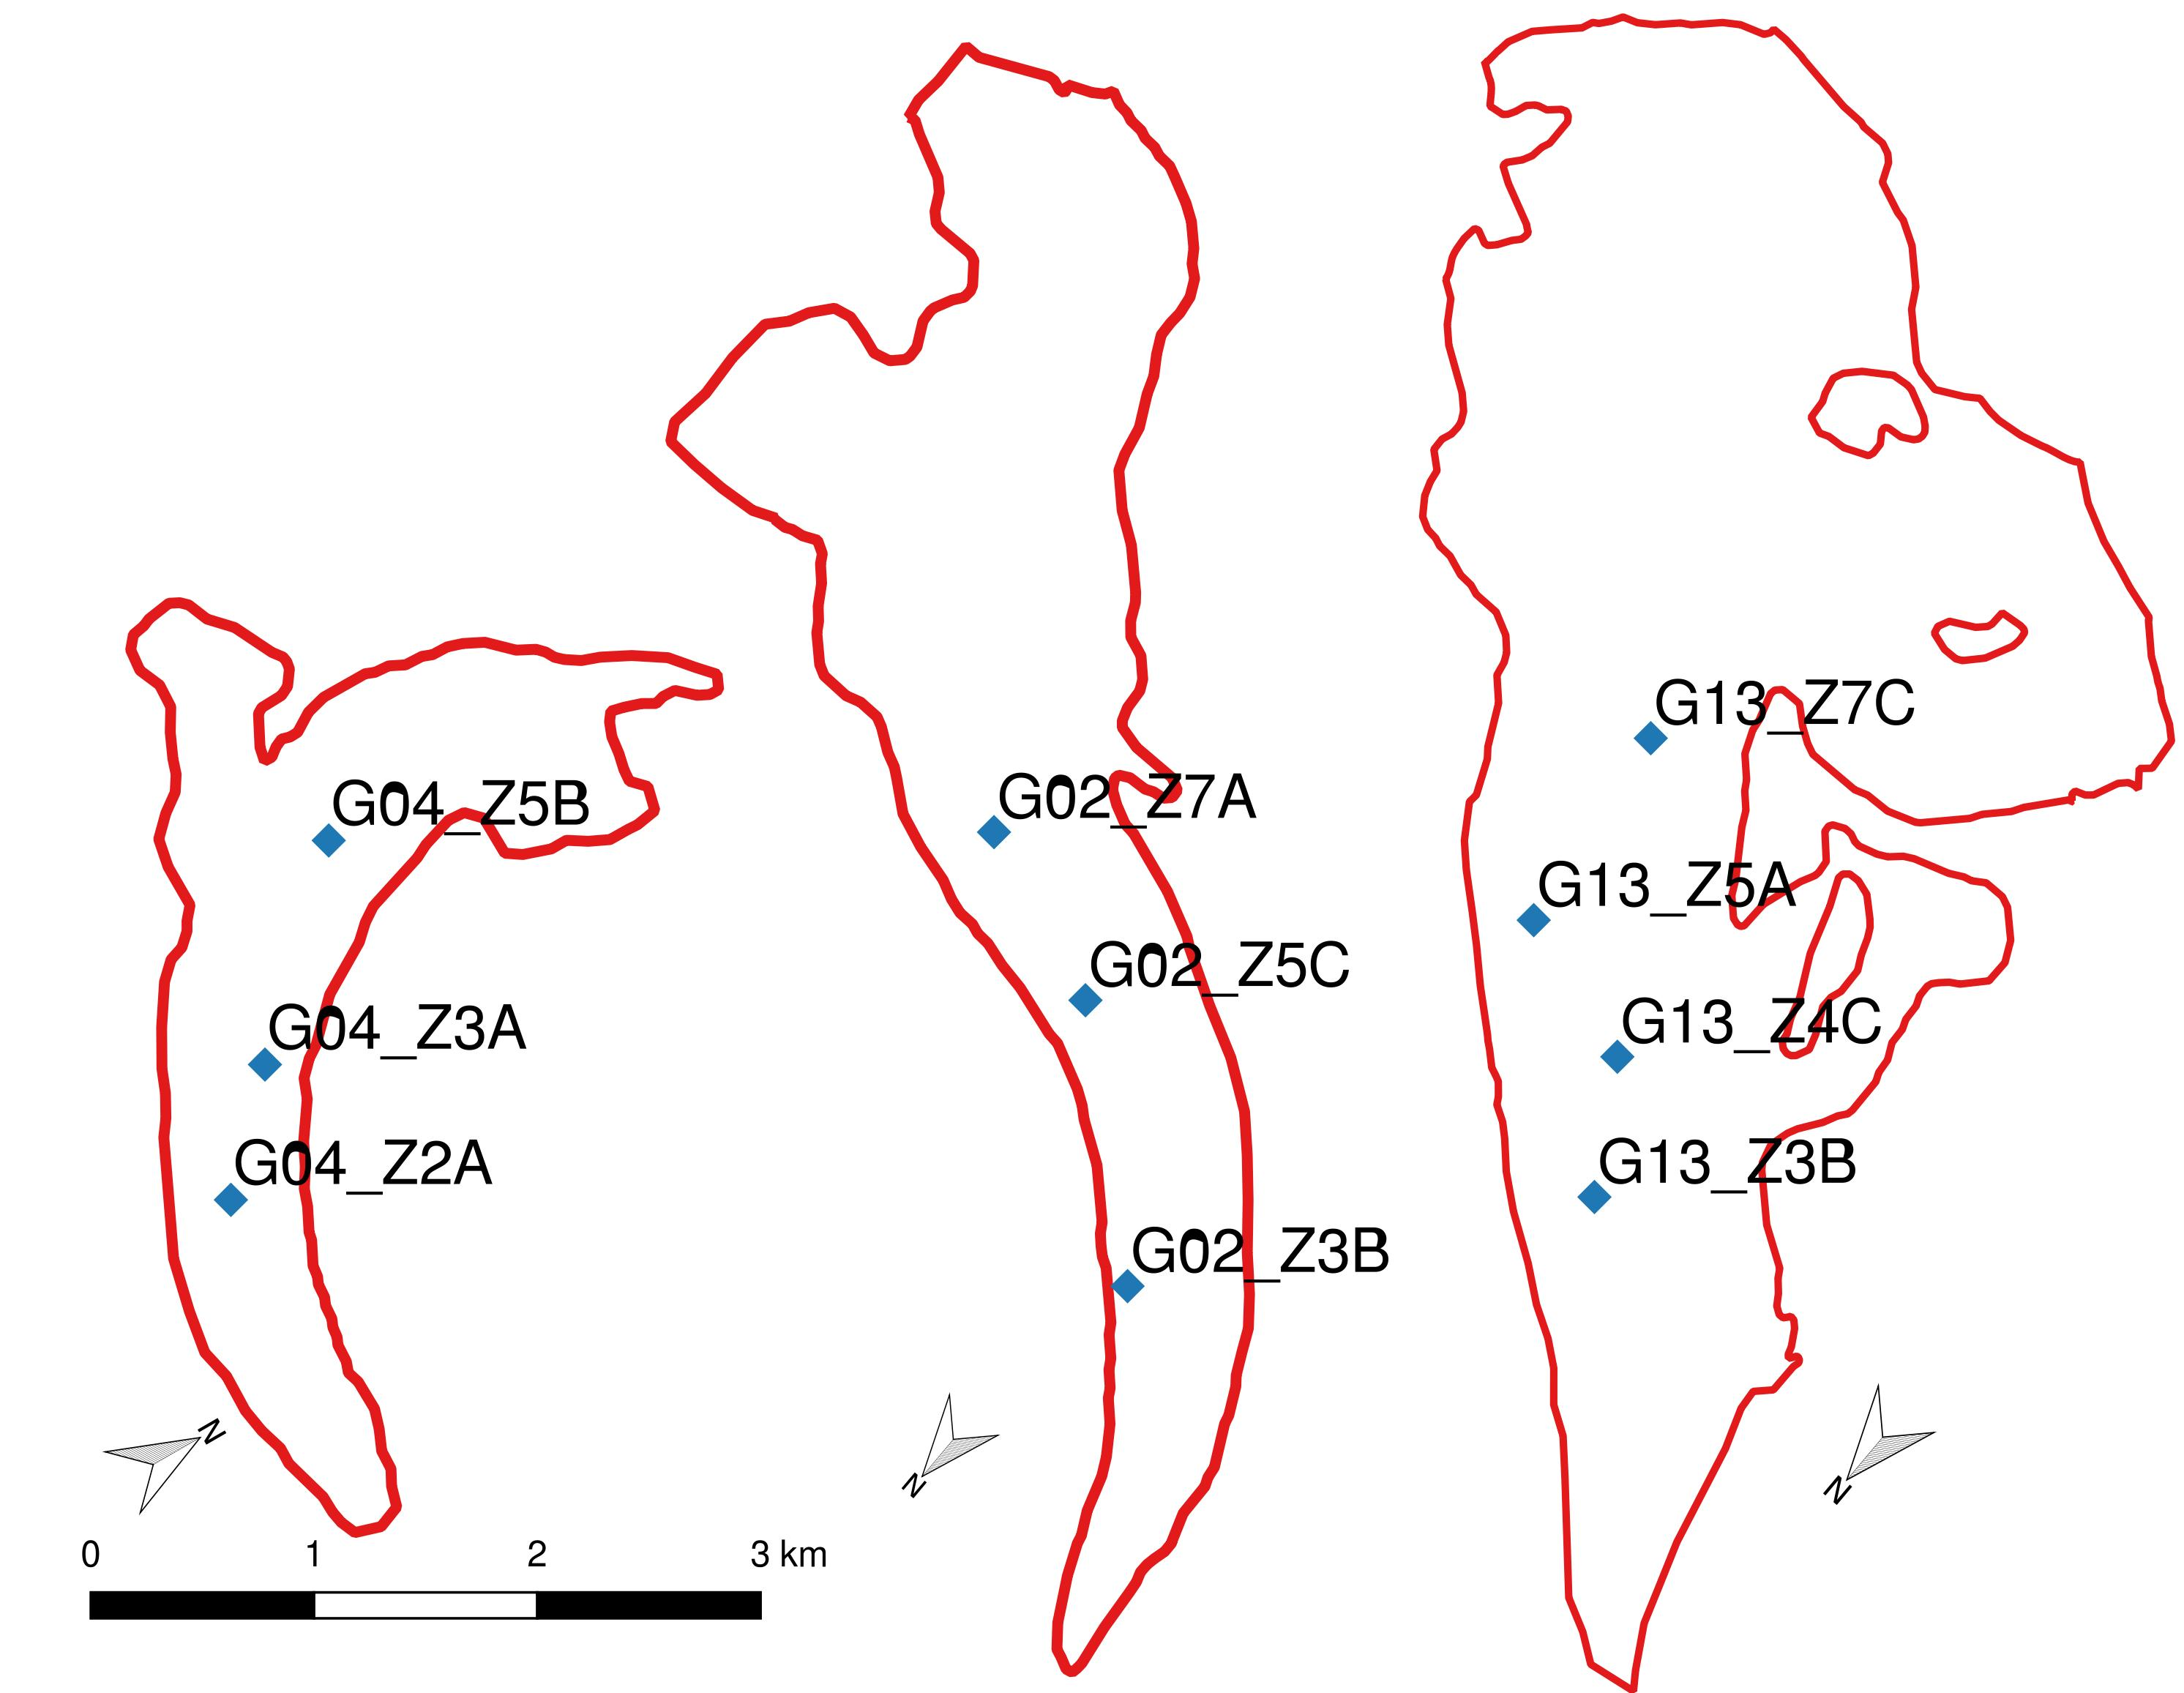
\includegraphics[width = 0.7\textwidth]{map_zigzaglocation_all.jpeg}\\
	\caption{Map of zigzag locations on Glaciers 4, 2 and 13 (left to right).}
	\label{fig:ZZ_locations}
\end{figure}

\begin{figure}[H]
	\centering
	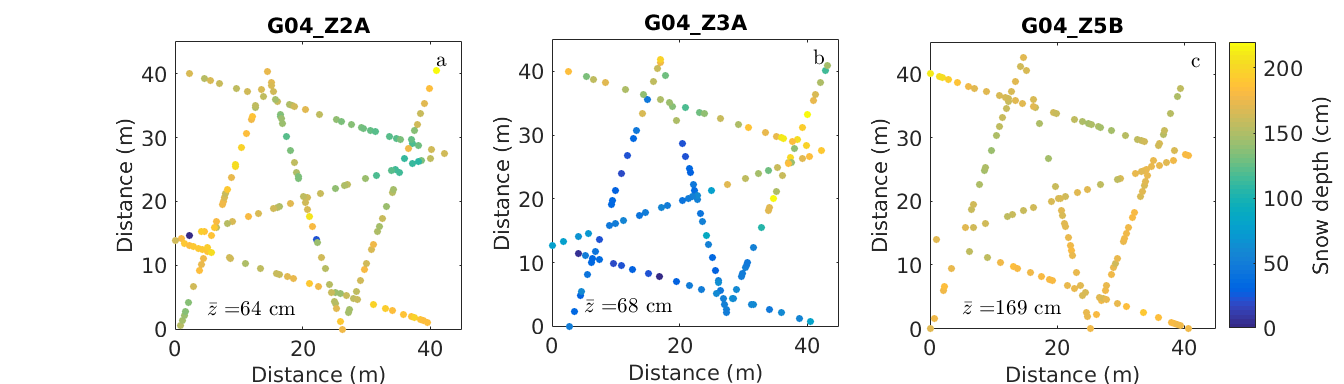
\includegraphics[width = \textwidth]{ZigzagDepth_G04.png}\\
	\caption{Snow depths measured in zigzags on Glacier 4. Mean depth ($\bar{z}$) is also reported. Zigzag elevations (left to right) are 2162, 2229 and 2360 \,m\,a.s.l. See Figure \ref{fig:ZZ_locations} for locations of each zigzag.}
	\label{fig:ZZ_G04}
\end{figure}

\begin{figure}[H]
	\centering
	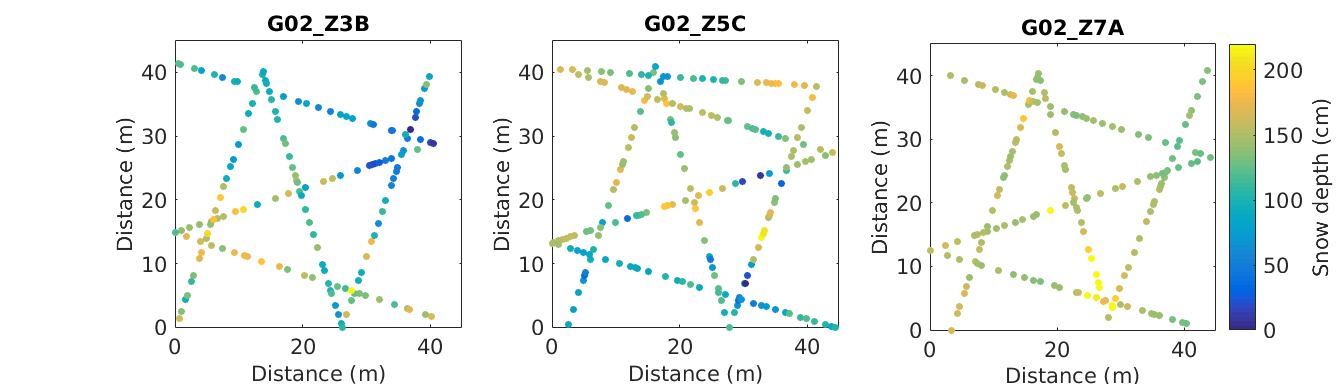
\includegraphics[width = \textwidth]{ZigzagDepth_G02.png}\\
	\caption{Snow depths measured in  zigzags on Glacier 2. Mean depth ($\bar{z}$) is also reported. Zigzag elevations (left to right) are 2172, 2332 and 2403 \,m\,a.s.l. See Figure \ref{fig:ZZ_locations} for locations of each zigzag.}
	\label{fig:ZZ_G02}
\end{figure}

\begin{figure}[H] 
	\centering
	 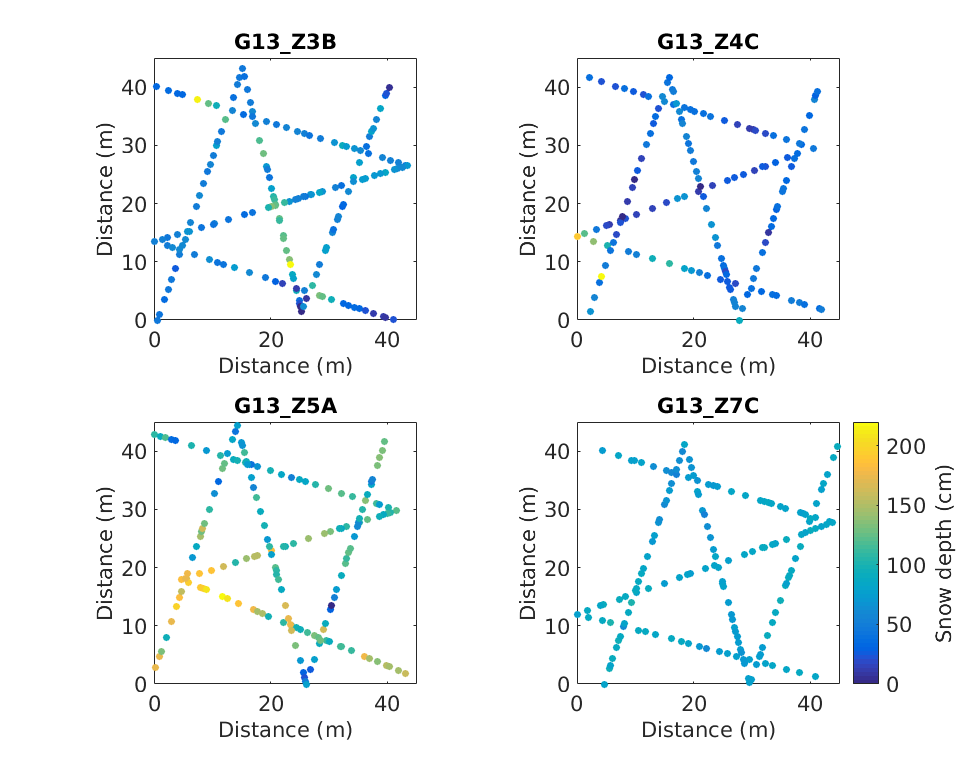
\includegraphics[width=0.9\textwidth]{ZigzagDepth_G13.png}%
	\caption{Snow depths measured in zigzags on Glacier 13. Mean depth ($\bar{z}$) is also reported. Zigzag elevations (a-d) are 2156, 2206, 2271 and 2297 \,m\,a.s.l. See Figure \ref{fig:ZZ_locations} for locations of each zigzag.}
	\label{fig:ZZ_G13}
\end{figure}


%%%%%%%%%%%%%%%%%%%%%%%%%%%%%%%%%%%%%%
\section{Point-scale winter balance}

Point-scale winter balance (WB) at sampling locations is estimated using eight density assignment methods (Section \ref{sec:density}). Groups of data, each calculated with a different density assignment method, are tested for differences using analysis of variance (ANOVA with p$<$0.05). Estimates of point-scale WB on each glacier are significantly different when various density assignment methods are applied (Figure \ref{fig:AllSWEopts_boxplot}). Glacier 4 has two main groups of point-scale WB estimates with a number of estimates that overlap (belong to both group A and C). The estimate calculated using F1 has a lower mean than the remaining estimates. Glacier 2 has four different groups of point-scale WB estimates but all estimates belong to multiple groups so there is no one estimate that differs from the rest. Point-scale WB estimates on Glacier 13 found using FS-derived densities (group B) have a higher mean than those found using SP-derived densities (groups A, C and D). The percent difference between the means of the point-scale WB estimates are 12\%, 18\% and 19\%  for Glacier 4, 2 and 13, respectively. 

Density assignment method 3 (Figures \ref{fig:SWEmap_S3} and \ref{fig:SWEmap_F3}), which uses a linear regression of density on elevation (S3 and F3), is used in this study to examine how a regression based on topography could affect point-scale WB estimates. Despite relationships of opposite sign between density and elevation for FS-derived densities and SP-derived densities (Table \ref{tab:elev_regress}), the point-scale WB estimates do not differ significantly for Glaciers 4 and 2. On Glacier 13, S3 and F3 point-scale WB estimates do differ but all point-scale WB estimates with FS-derived densities differ from point-scale WB estimates with SP-derived densities. This systematic difference is perhaps a result of undersampling by the FS on Glacier 13. Undersampling could have occurred because a considerable portion of the snowpack had undergone melt and snow depths were commonly low, potentially resulting in snow falling out of the sampling tube. 

For all density assignment methods, point-scale WB is highest on Glacier 4 and lowest on Glacier 13. Glacier 4 also shows considerable point-scale WB variability within the basin, with both high and low values along a single transect (Figures \ref{fig:SWEmap_S1} to \ref{fig:SWEmap_F4}). The northwest side of Glacier 2 has low values of point-scale WB with large variations along transects. During field data collection, this area was observed to have a surface texture characterized by roughness elements that were $\sim$2\,m wide and long and $\sim$0.5\,m tall with exposed ice on the ridge crests and wind-deposited snow patches in troughs.



\begin{figure}[H]
	\centering
	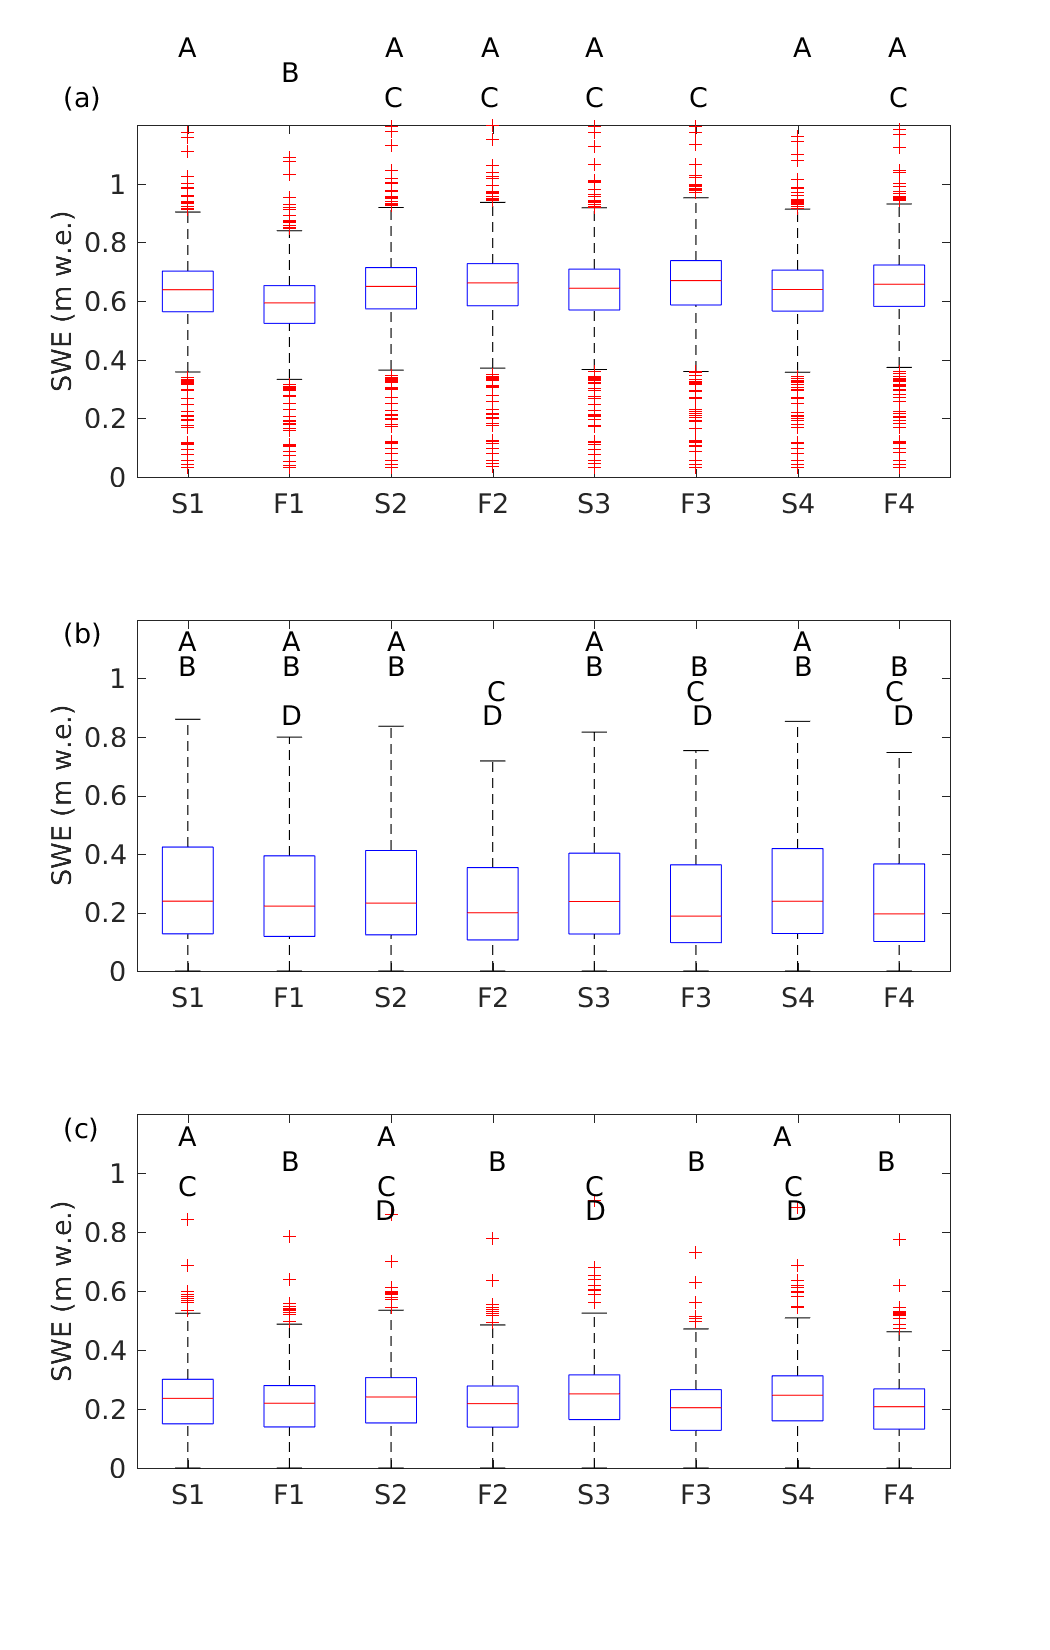
\includegraphics[width = 0.8\textwidth]{AllSWEopts_boxplot.png}\\
	\caption{Boxplots of estimated point-scale winter balance (WB) at sampling locations for (a) Glacier 4, (b) Glacier 2 and (c) Glacier 13. See Table \ref{tab:densityOptions} for explanation of density assignment methods and codes. Point-scale WB estimates using various density assignment methods were tested for differences using ANOVA (p$<$0.05). Point-scale WB estimates that were not significantly different are labelled with the same letter (e.g. all estimates with A on Glacier 4 are significantly different than all estimates with B on Glacier 4).}
	\label{fig:AllSWEopts_boxplot}
\end{figure}


\begin{figure}[H]
	\centering
	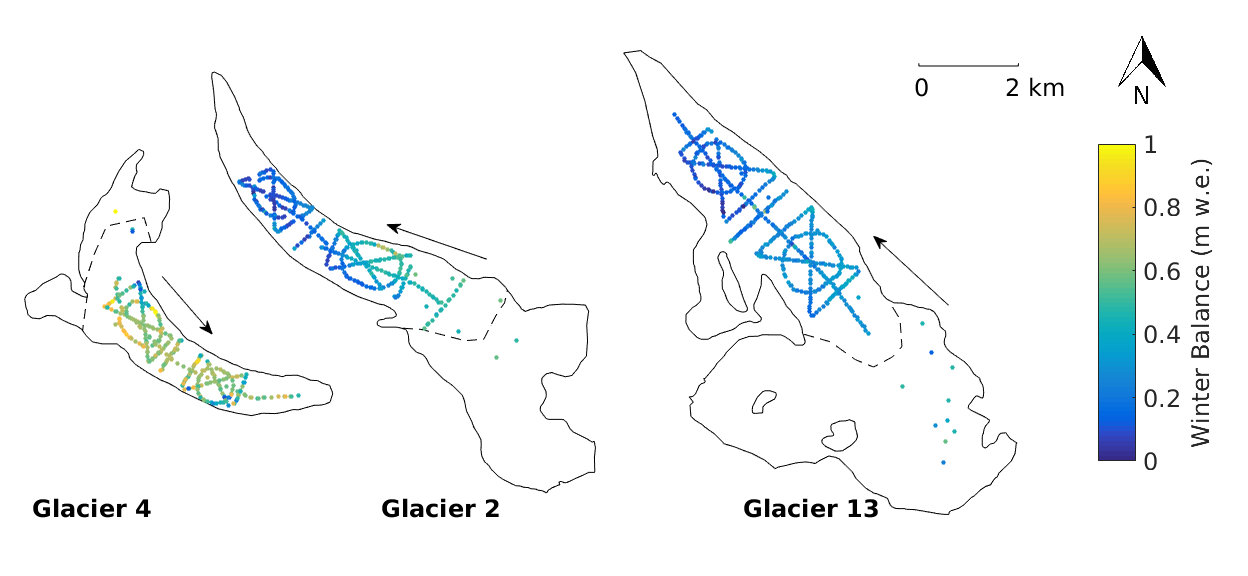
\includegraphics[width = \textwidth]{SWEmap_opt2.png}\\
	\caption{Estimated point-scale winter balance at measurement locations. Density was taken to be the mean value of all snow-pit-derived densities from all glaciers (S1). Arrows show ice-flow direction and dashed lines show approximate ELA. Note that the individual measurement locations overlap on the figure.}
	\label{fig:SWEmap_S1}
\end{figure}

\begin{figure}[H]
	\centering
	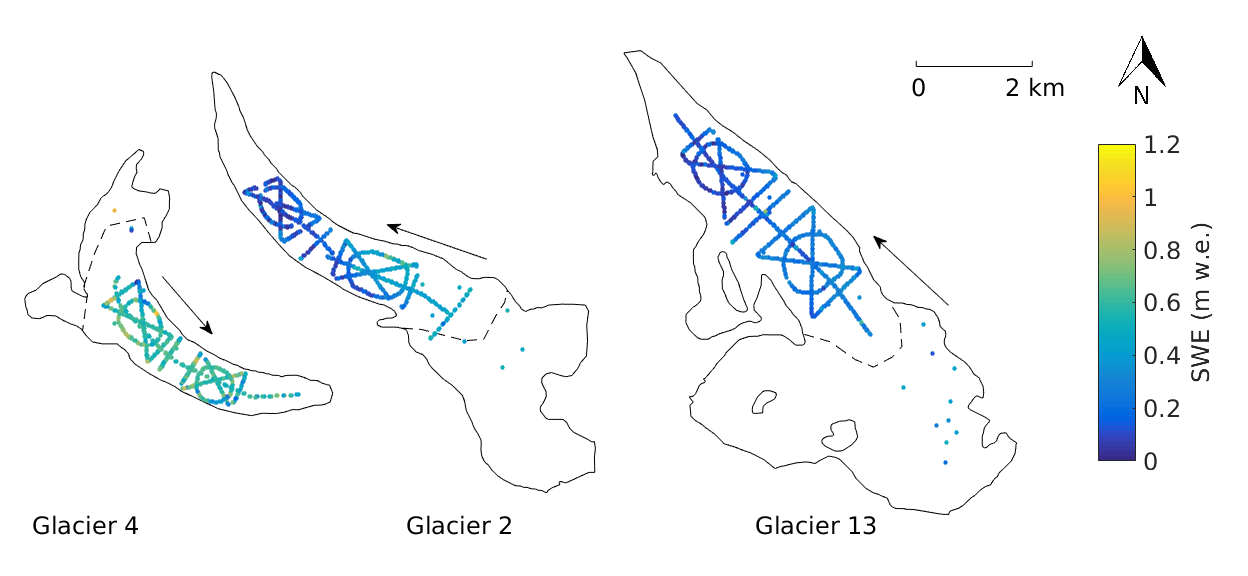
\includegraphics[width = \textwidth]{SWEmap_opt3.png}\\
	\caption{Estimated point-scale winter balance at measurement locations. Density was taken to be the mean value of all Federal-Sampler-derived densities from all glaciers (F1). Arrows show ice-flow direction and dashed lines show approximate ELA. Note that the individual measurement locations overlap on the figure.}
	\label{fig:SWEmap_F1}
\end{figure}

\begin{figure}[H]
	\centering
	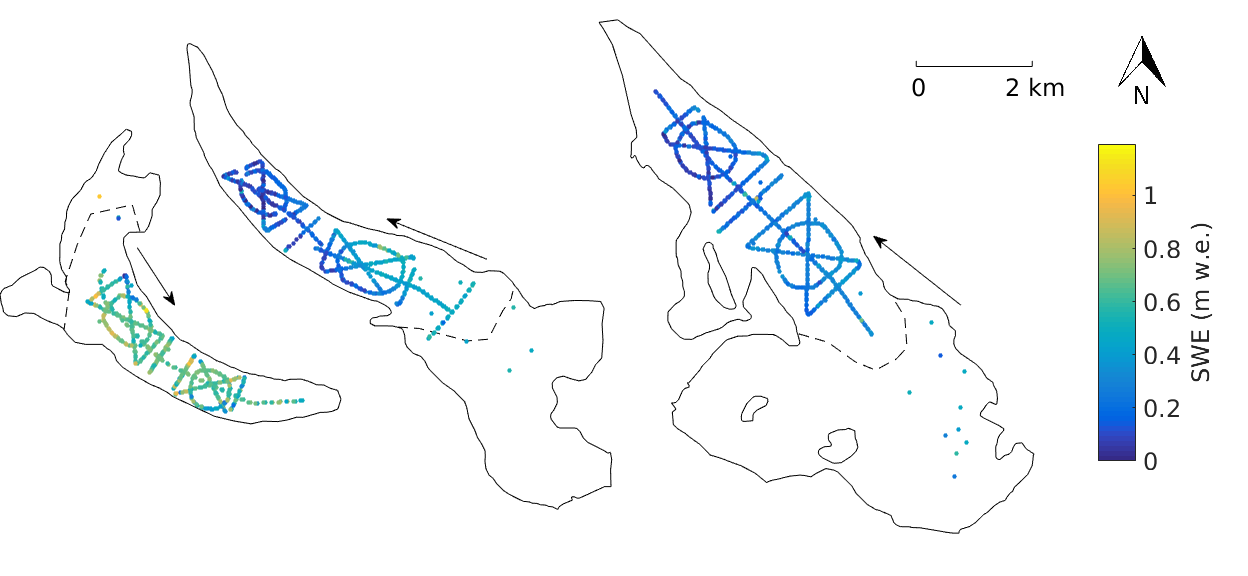
\includegraphics[width =\textwidth]{SWEmap_opt4.png}\\
	\caption{Estimated point-scale winter balance at measurement locations. Density for each glacier was taken to be the mean value of snow-pit-derived densities from that glacier (S2). Arrows show ice-flow direction and dashed lines show approximate ELA. Note that the individual measurement locations overlap on the figure.}
	\label{fig:SWEmap_S2}
\end{figure}

\begin{figure}[H]
	\centering
	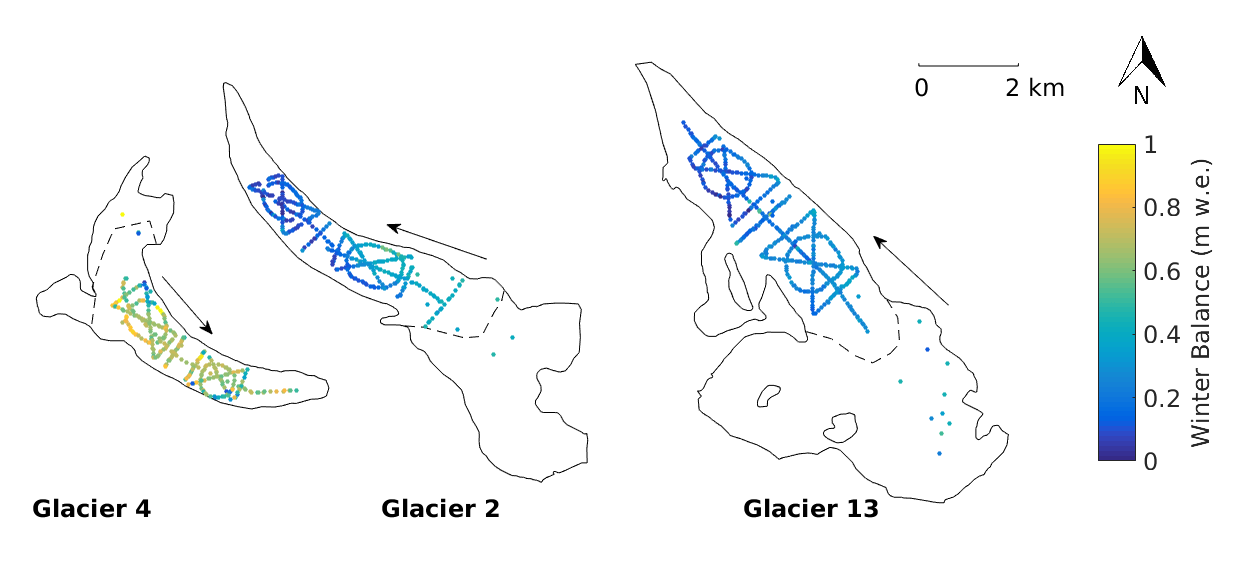
\includegraphics[width = \textwidth]{SWEmap_opt5.png}\\
	\caption{Estimated point-scale winter balance at measurement locations. Density for each glacier was taken to be the mean value of Federal-Sampler-derived densities from that glacier (F2). Arrows show ice-flow direction and dashed lines show approximate ELA. Note that the individual measurement locations overlap on the figure.}
	\label{fig:SWEmap_F2}
\end{figure}

\begin{figure}[H]
	\centering
	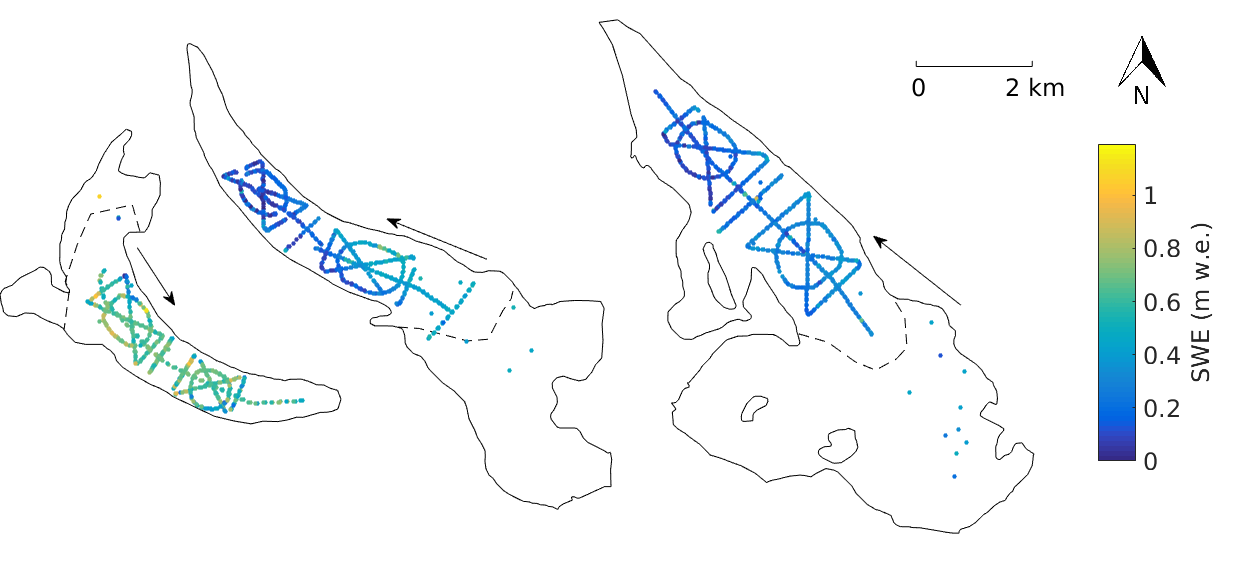
\includegraphics[width = \textwidth]{SWEmap_opt6.png}\\
	\caption{Estimated point-scale winter balance at measurement locations. Density was determined by using a linear fit between snow-pit-derived density and elevation for each glacier (S3). Arrows show ice-flow direction and dashed lines show approximate ELA. Note that the individual measurement locations overlap on the figure.}
	\label{fig:SWEmap_S3}
\end{figure}

\begin{figure}[H]
	\centering
	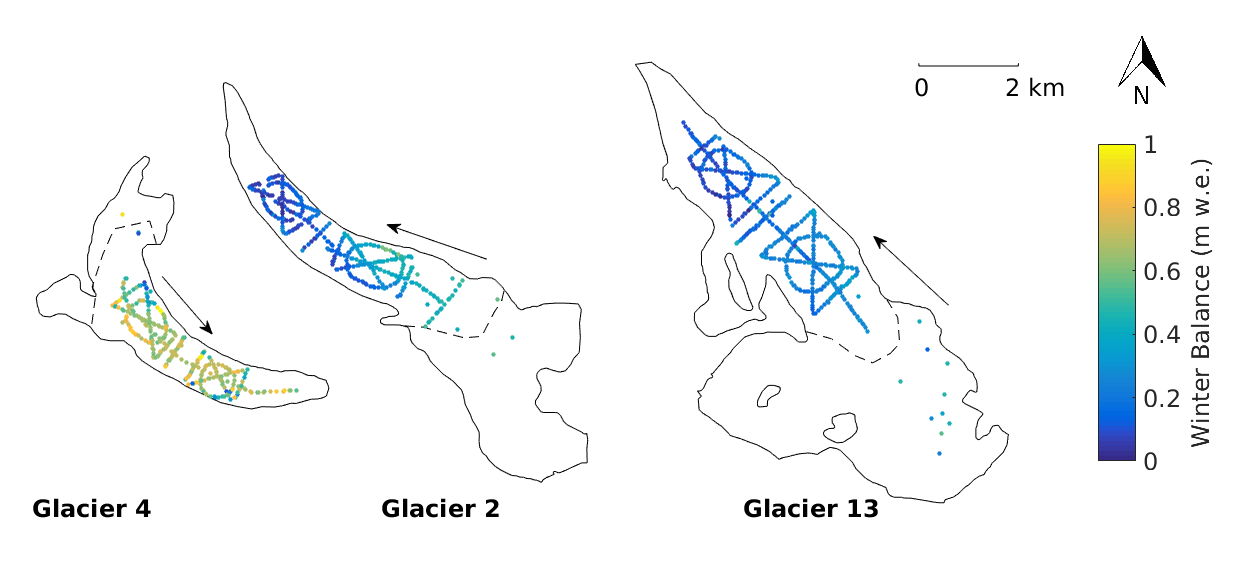
\includegraphics[width = \textwidth]{SWEmap_opt7.png}\\
	\caption{Estimated point-scale winter balance at measurement locations.Density was determined by using a linear fit between Federal-Sampler-derived density and elevation for each glacier (F3). Arrows show ice-flow direction and dashed lines show approximate ELA. Note that the individual measurement locations overlap on the figure.}
	\label{fig:SWEmap_F3}
\end{figure}

\begin{figure}[H]
	\centering
	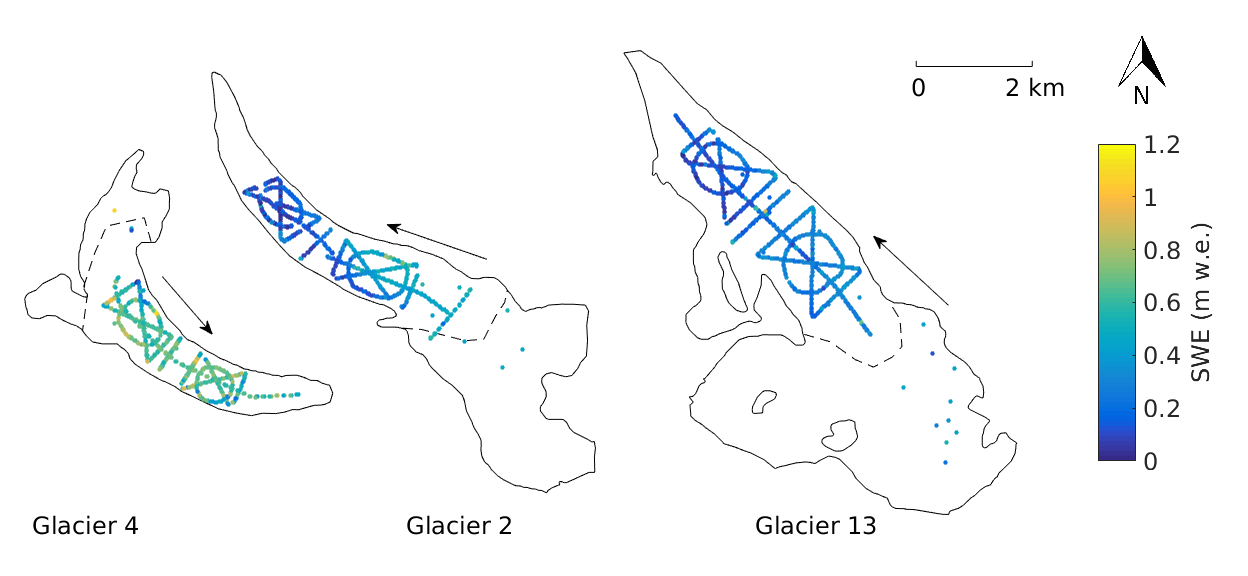
\includegraphics[width = \textwidth]{SWEmap_opt8.png}\\
	\caption{Estimated point-scale winter balance at measurement locations. Density was calculated using inverse distance weighting using all snow-pit-derived densities (S4). Arrows show ice-flow direction and dashed lines show approximate ELA. Note that the individual measurement locations overlap on the figure.}
	\label{fig:SWEmap_S4}
\end{figure}

\begin{figure}[H]
	\centering
	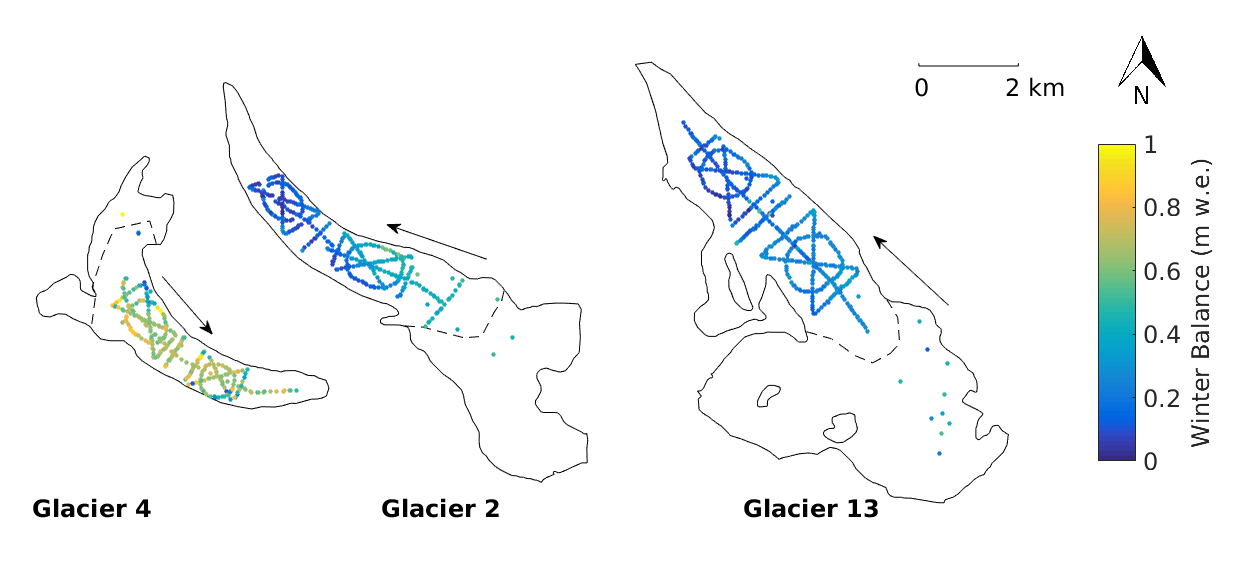
\includegraphics[width =\textwidth]{SWEmap_opt9.png}\\
	\caption{Estimated point-scale winter balance at measurement locations. Density was calculated using inverse distance weighting using all snow-pit-derived densities (F4). Arrows show ice-flow direction and dashed lines show approximate ELA. Note that the individual measurement locations overlap on the figure.}
	\label{fig:SWEmap_F4}
\end{figure}


\section{Summary}

In this chapter, snow depth and density data are investigated. First, density values derived from snow pit (SP) and Federal Sampler (FS) measurements are compared. FS-derived densities are found to be correlated with snow depth and I establish that the FS is likely oversampling in deep snow and undersampling in shallow snow. Contrary to expectation, co-located FS and SP measurements are found to be uncorrelated. Relationships between density and elevation differ in magnitude and sign between density measurement methods and between glaciers. Assessed uncertainties in density values are found to be small (usually $<$10\%). I then investigate collected snow depth data at multiple scales. From the transect surveys, Glacier 4 has the highest mean value and the largest range of observed snow depth, while Glacier 13 has the lowest mean value and smallest range. Zigzag survey data indicate that the range of snow depths within a gridcell is comparable between gridcells but that some gridcells have many outliers. Point-scale WB analysis indicates that the density assignment method creates significant, but inconsistent, differences in glacier-wide WB. 

%%%%
\chapter{Digital elevation models and topographic parameters}
%%%%

This chapter documents how topographic parameters are obtained from a given DEM of the study region. Processing steps such as DEM stitching, smoothing and raster calculations are described in detail.  Appendix \ref{app:topoparams_QGIS_Matlab} describes how to import topographic parameters from QGIS to Matlab. 

\section{DEMs for the study glaciers}

Topographic parameters are derived from a digital elevation model (DEM) of the study area. The DEM used in this project was created from imagery collected by the SPOT-5 satellite and it was provided at no cost by the French Space Agency (CNES) through the SPIRIT International Polar Year project \citep{Korona2009}. The DEM has a cell size of 40$\times$40 m. The DEM was created using a set of correlation parameters fit for steeper slopes (E. Berthier personal communication, 2016). 

Two DEMs are available for the Donjek Range. The first DEM (GES 08-029) was made from images collected on September 3, 2007 and the second DEM (GES 07-044) from images collected on September 13, 2007. The snow extent on September 13, 2007, as imaged by the Landsat 7 satellite, can be seen in Figure \ref{fig:Landsat_2007}. Since the images were collected in September, the snow would likely be at a seasonal minimum. Therefore, the surface described by the DEM in the ablation area represents the ice topography. A limitation in using this DEM is that it is from 2007 and there have almost certainly been changes in the end-of-summer glacier surface. However, the SPOT-5 DEM is the highest resolution and most current DEM available for the study area \footnote{At the time of project initiation, SPIRIT SPOT-5 was the highest resolution DEM available. At the time of completing this work, ArcticDEM and TanDEM-X are the highest resolution, freely-available DEMs available for the Donjek Range.}. 

\begin{figure}[H]
    \centering
    \begin{subfigure}[b]{0.48\textwidth}
        \fbox{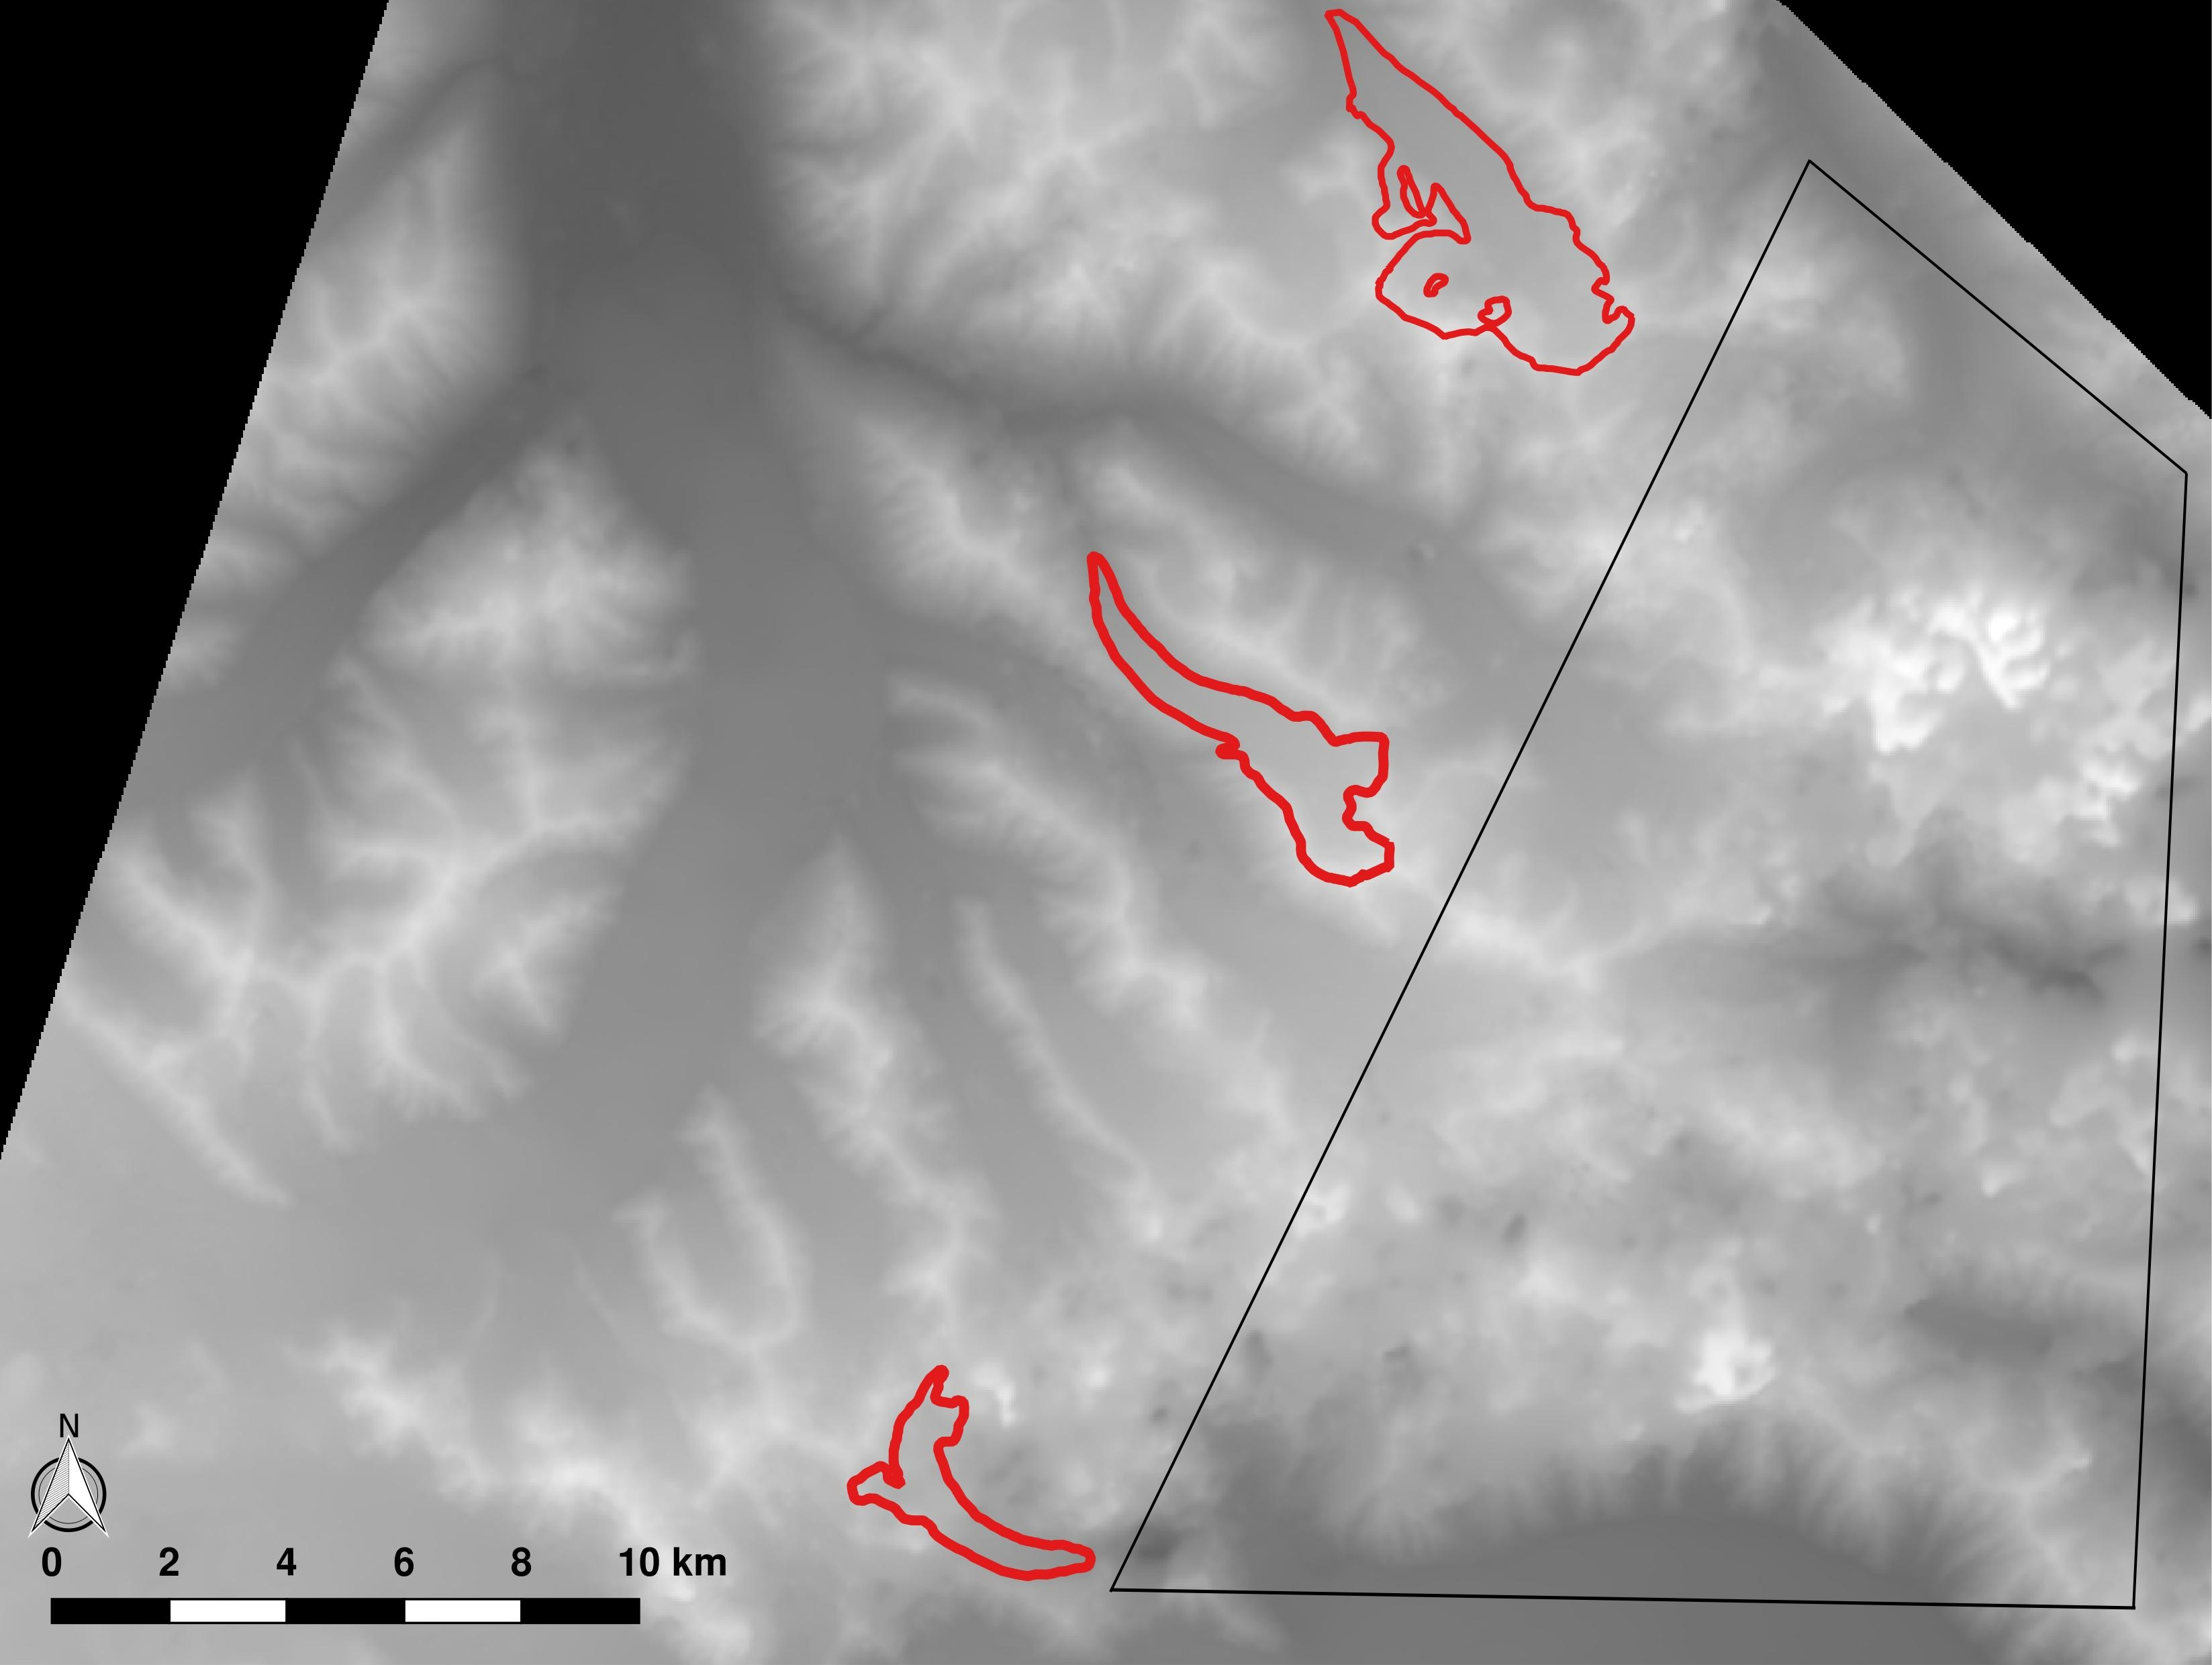
\includegraphics[width=\textwidth]{8029_original2.jpeg}}
        \caption{}
        \label{fig:8029_original}
    \end{subfigure}
    ~
    \begin{subfigure}[b]{0.48\textwidth}
        \fbox{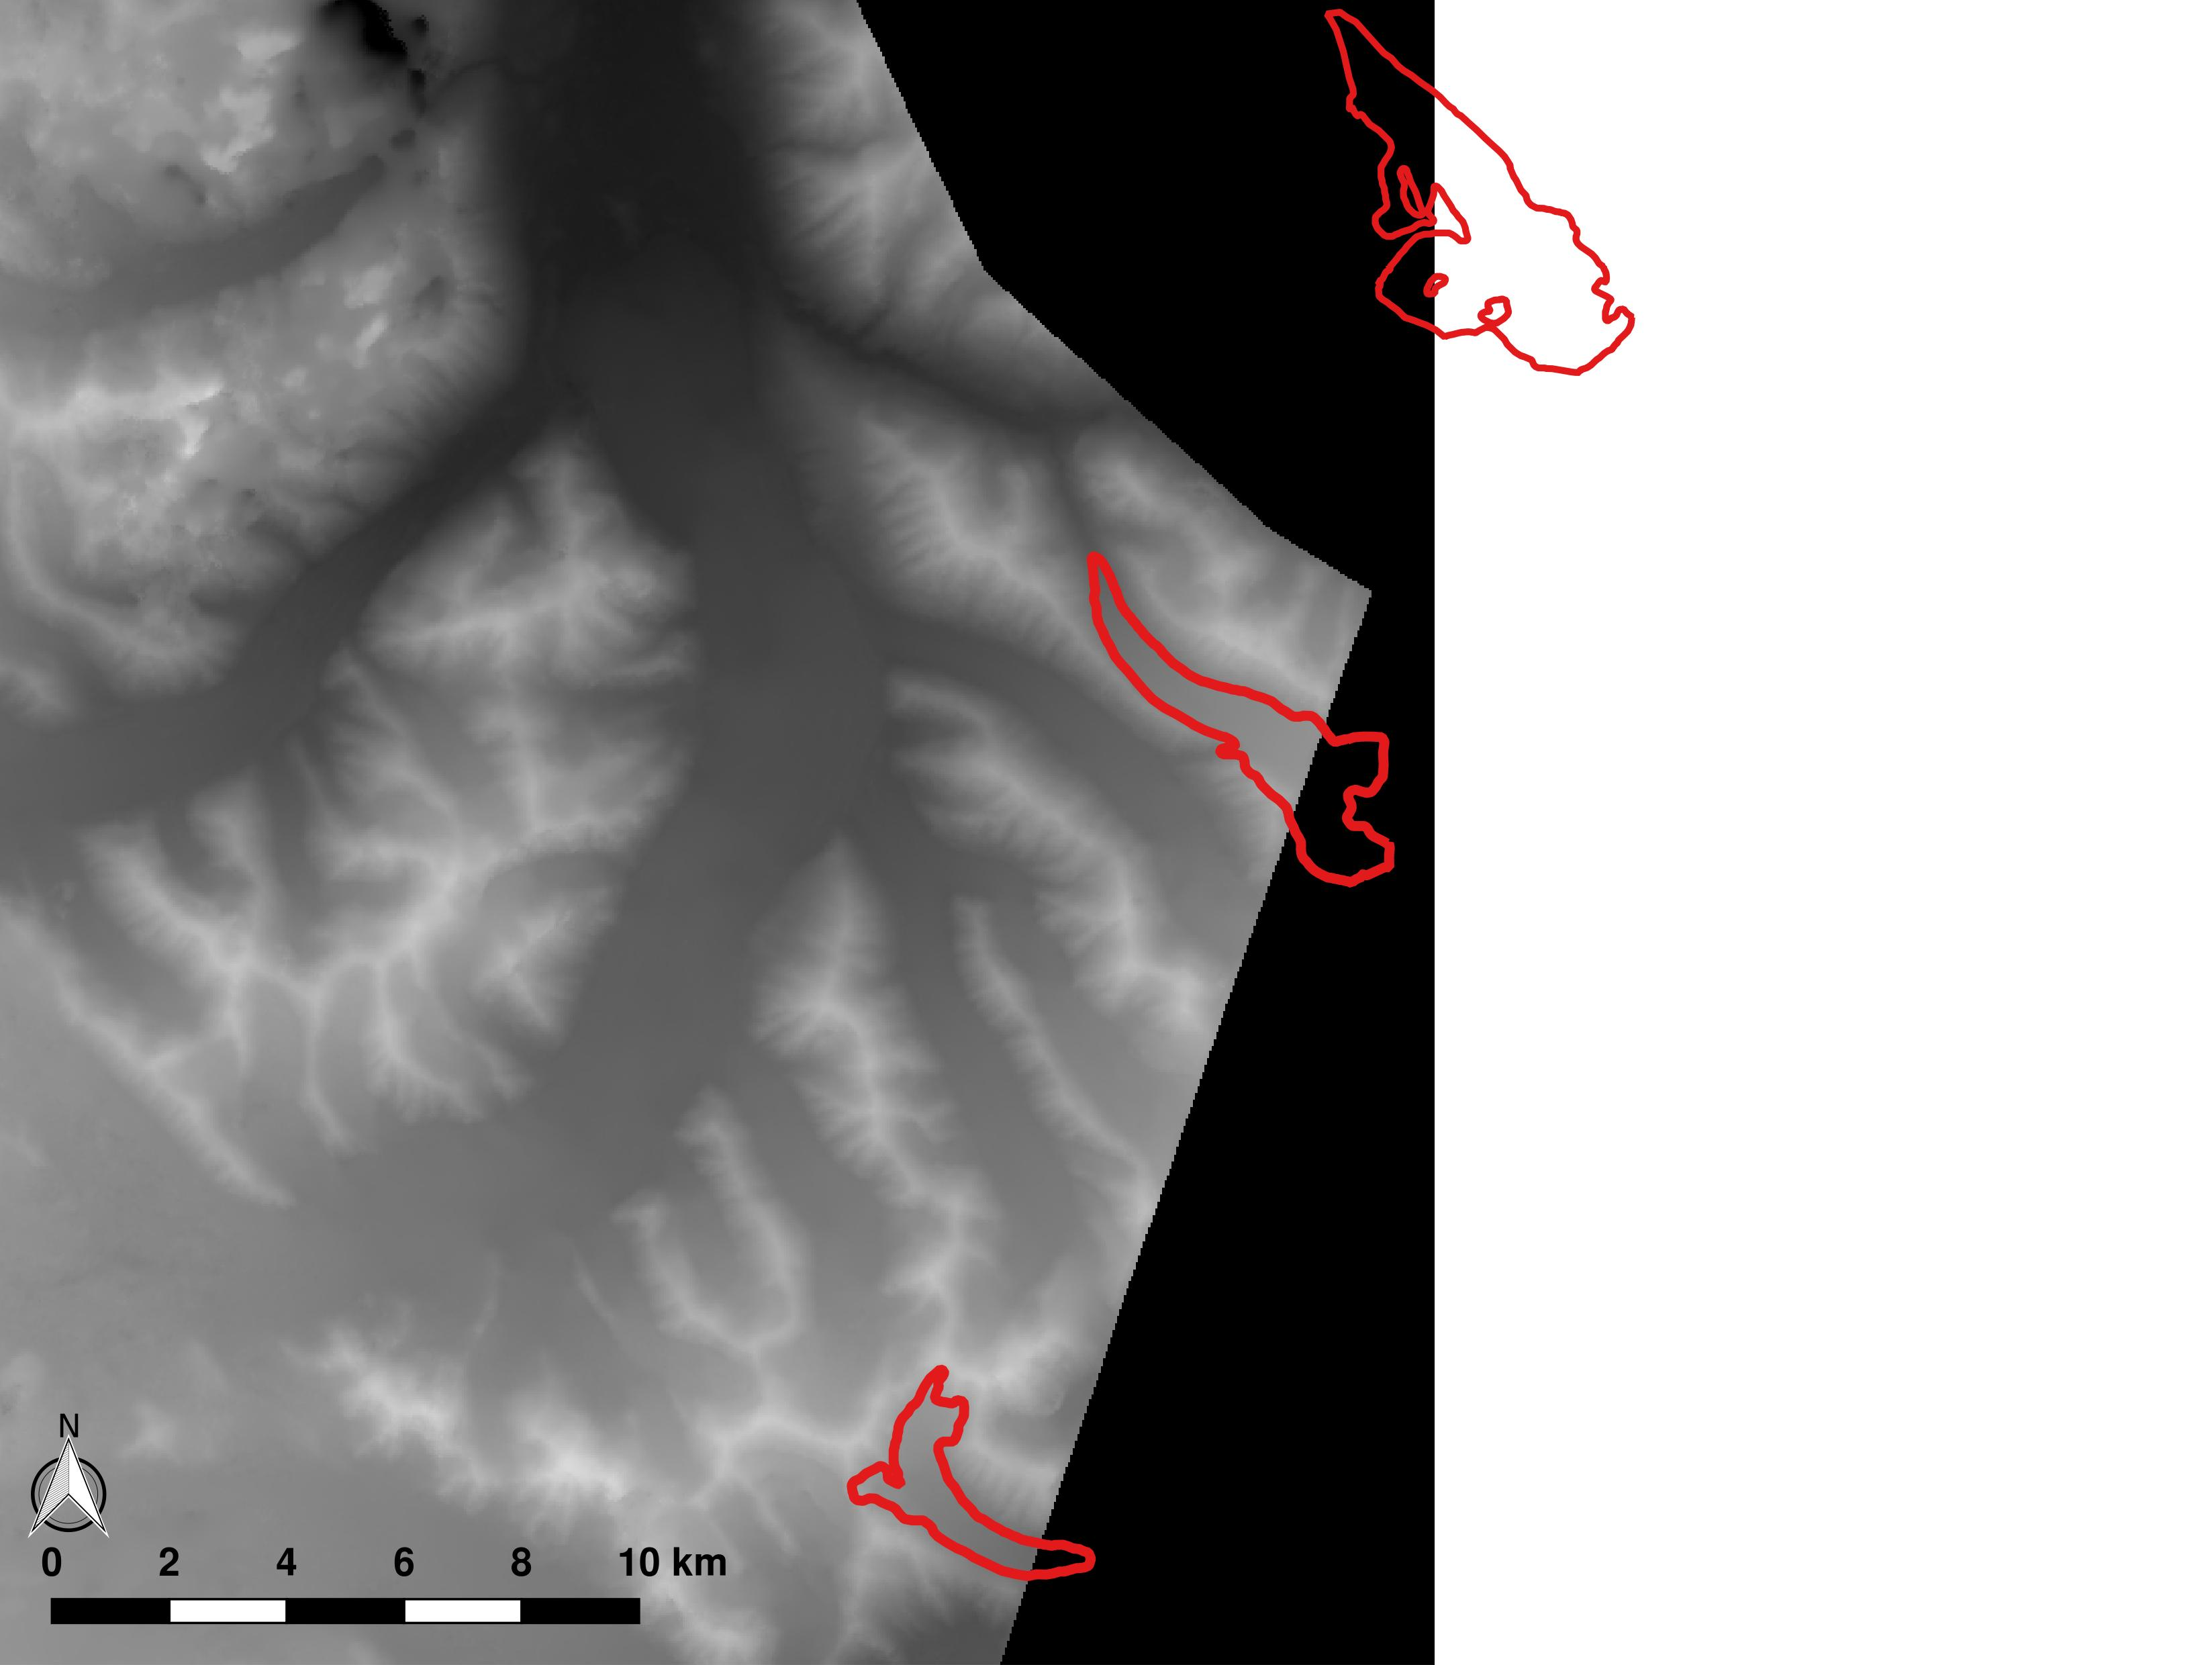
\includegraphics[width=\textwidth]{7044_original.jpeg}}
        \caption{}
        \label{fig:7044_original}
    \end{subfigure}

    \caption{SPOT-5 DEMs available for the Donjek Range. Study glaciers are shown as red outlines. The DEM made from imagery collected on September 3, 2007 (GES 08-029) is shown in (a) and the DEM made from imagery collected on September 13, 2007 (GES 07-044) is shown in (b). Imagery with cloud cover results in a distorted DEM, as seen in the boxed area of (a).}
    \label{fig:originalDEMs}
\end{figure}

\begin{figure}[H]
  \makebox[\textwidth][c]{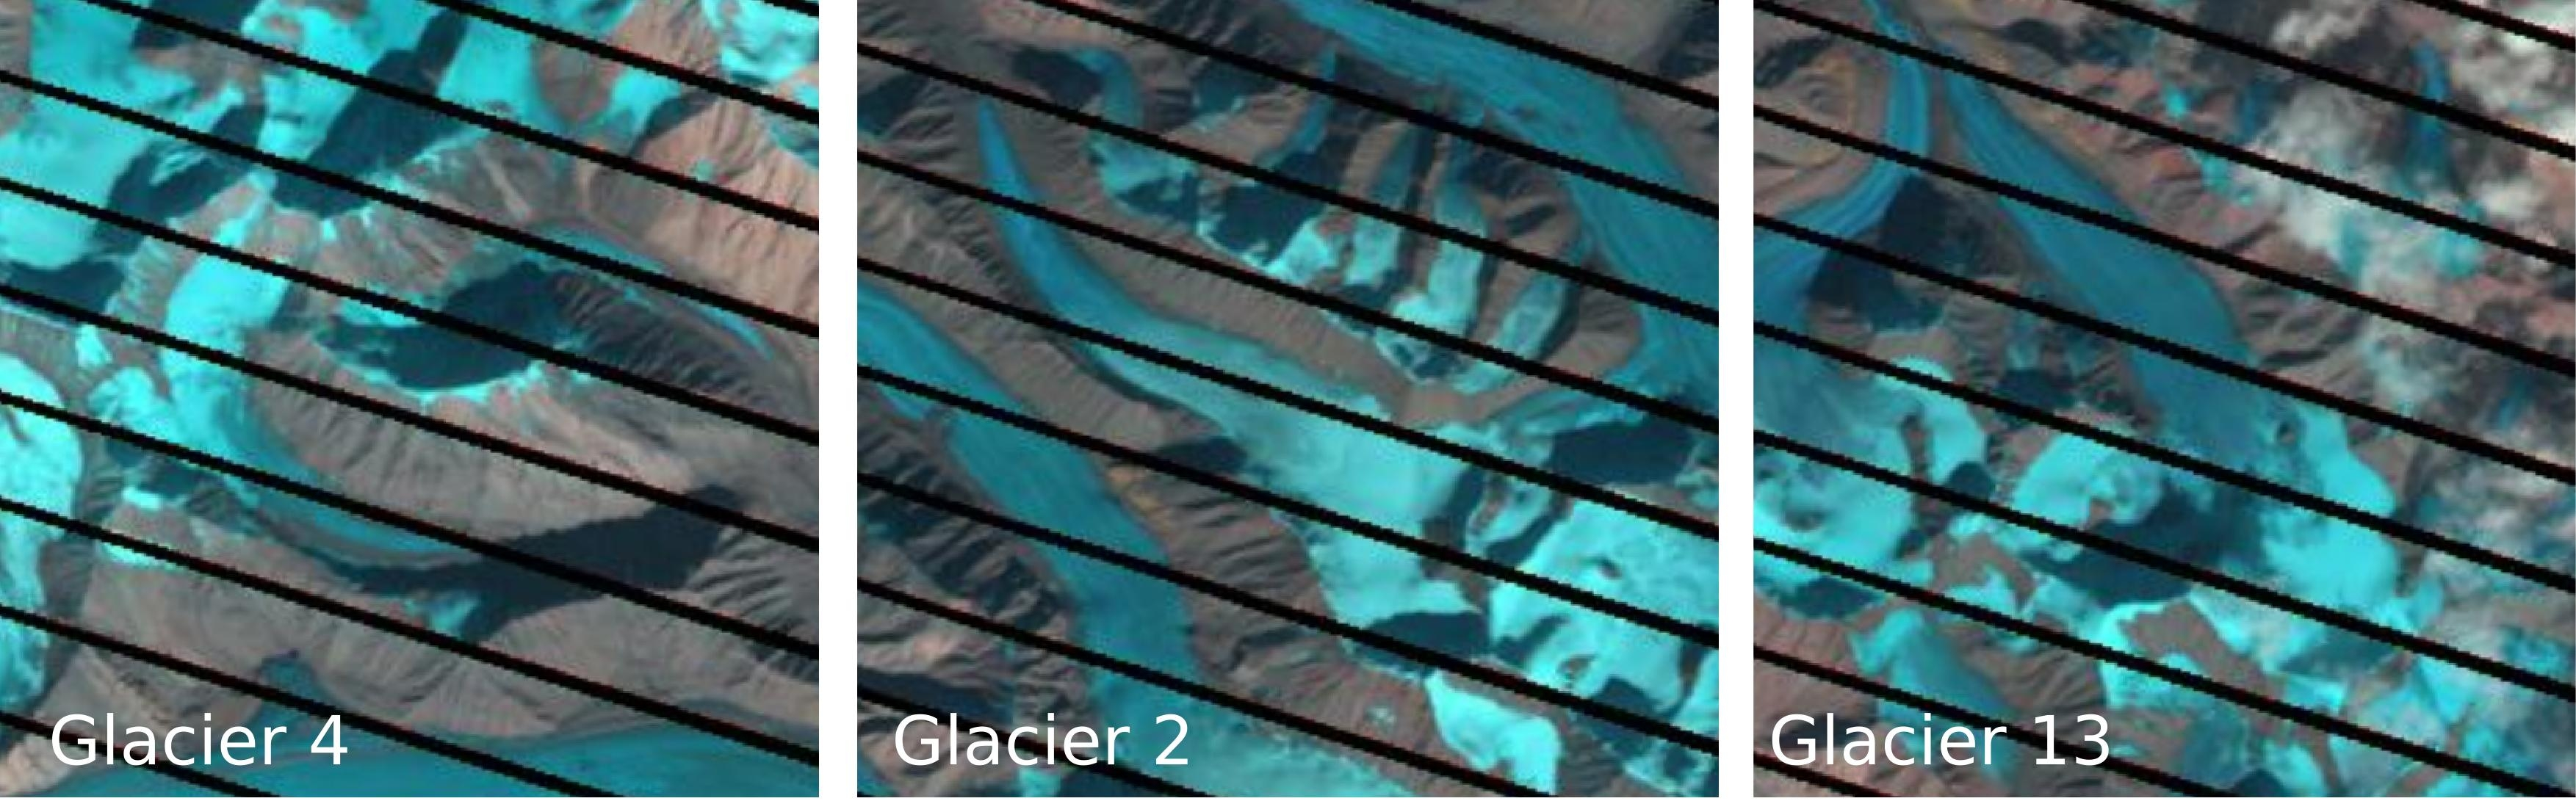
\includegraphics[width=\textwidth]{Landsat_2007.jpeg}}%
	\caption{Landsat 7 ETM images of study glaciers on September 13, 2007. Snow cover is shown as light blue and ice is shown as dark blue.}
	\label{fig:Landsat_2007}
\end{figure}

The GES 08-029 DEM covers all three study glaciers (see Figure \ref{fig:8029_original}) but a large part of Glacier 4 and some areas of Glacier 2 were masked by clouds and/or showed limited contrast in the original stero-image pairs, resulting in incorrect elevation data (E. Berthier personal communication, 2016). The cloudy areas appear as black regions in the DEM mask (not shown) and as distortion in the DEM, as seen in the boxed area of Figure \ref{fig:8029_original}. The second DEM (GES 07-044) spans only part of the Donjek Range, covering most of Glacier 4 and $\sim$60\% of Glacier 2 (see Figure \ref{fig:7044_original}). This DEM had no masked areas over Glaciers 2 and 4. The two DEMs were therefore merged to create a cloud-free DEM that spanned all three glaciers. 

\begin{figure}[H]
    \centering
    \begin{subfigure}[b]{0.48\textwidth}
        \fbox{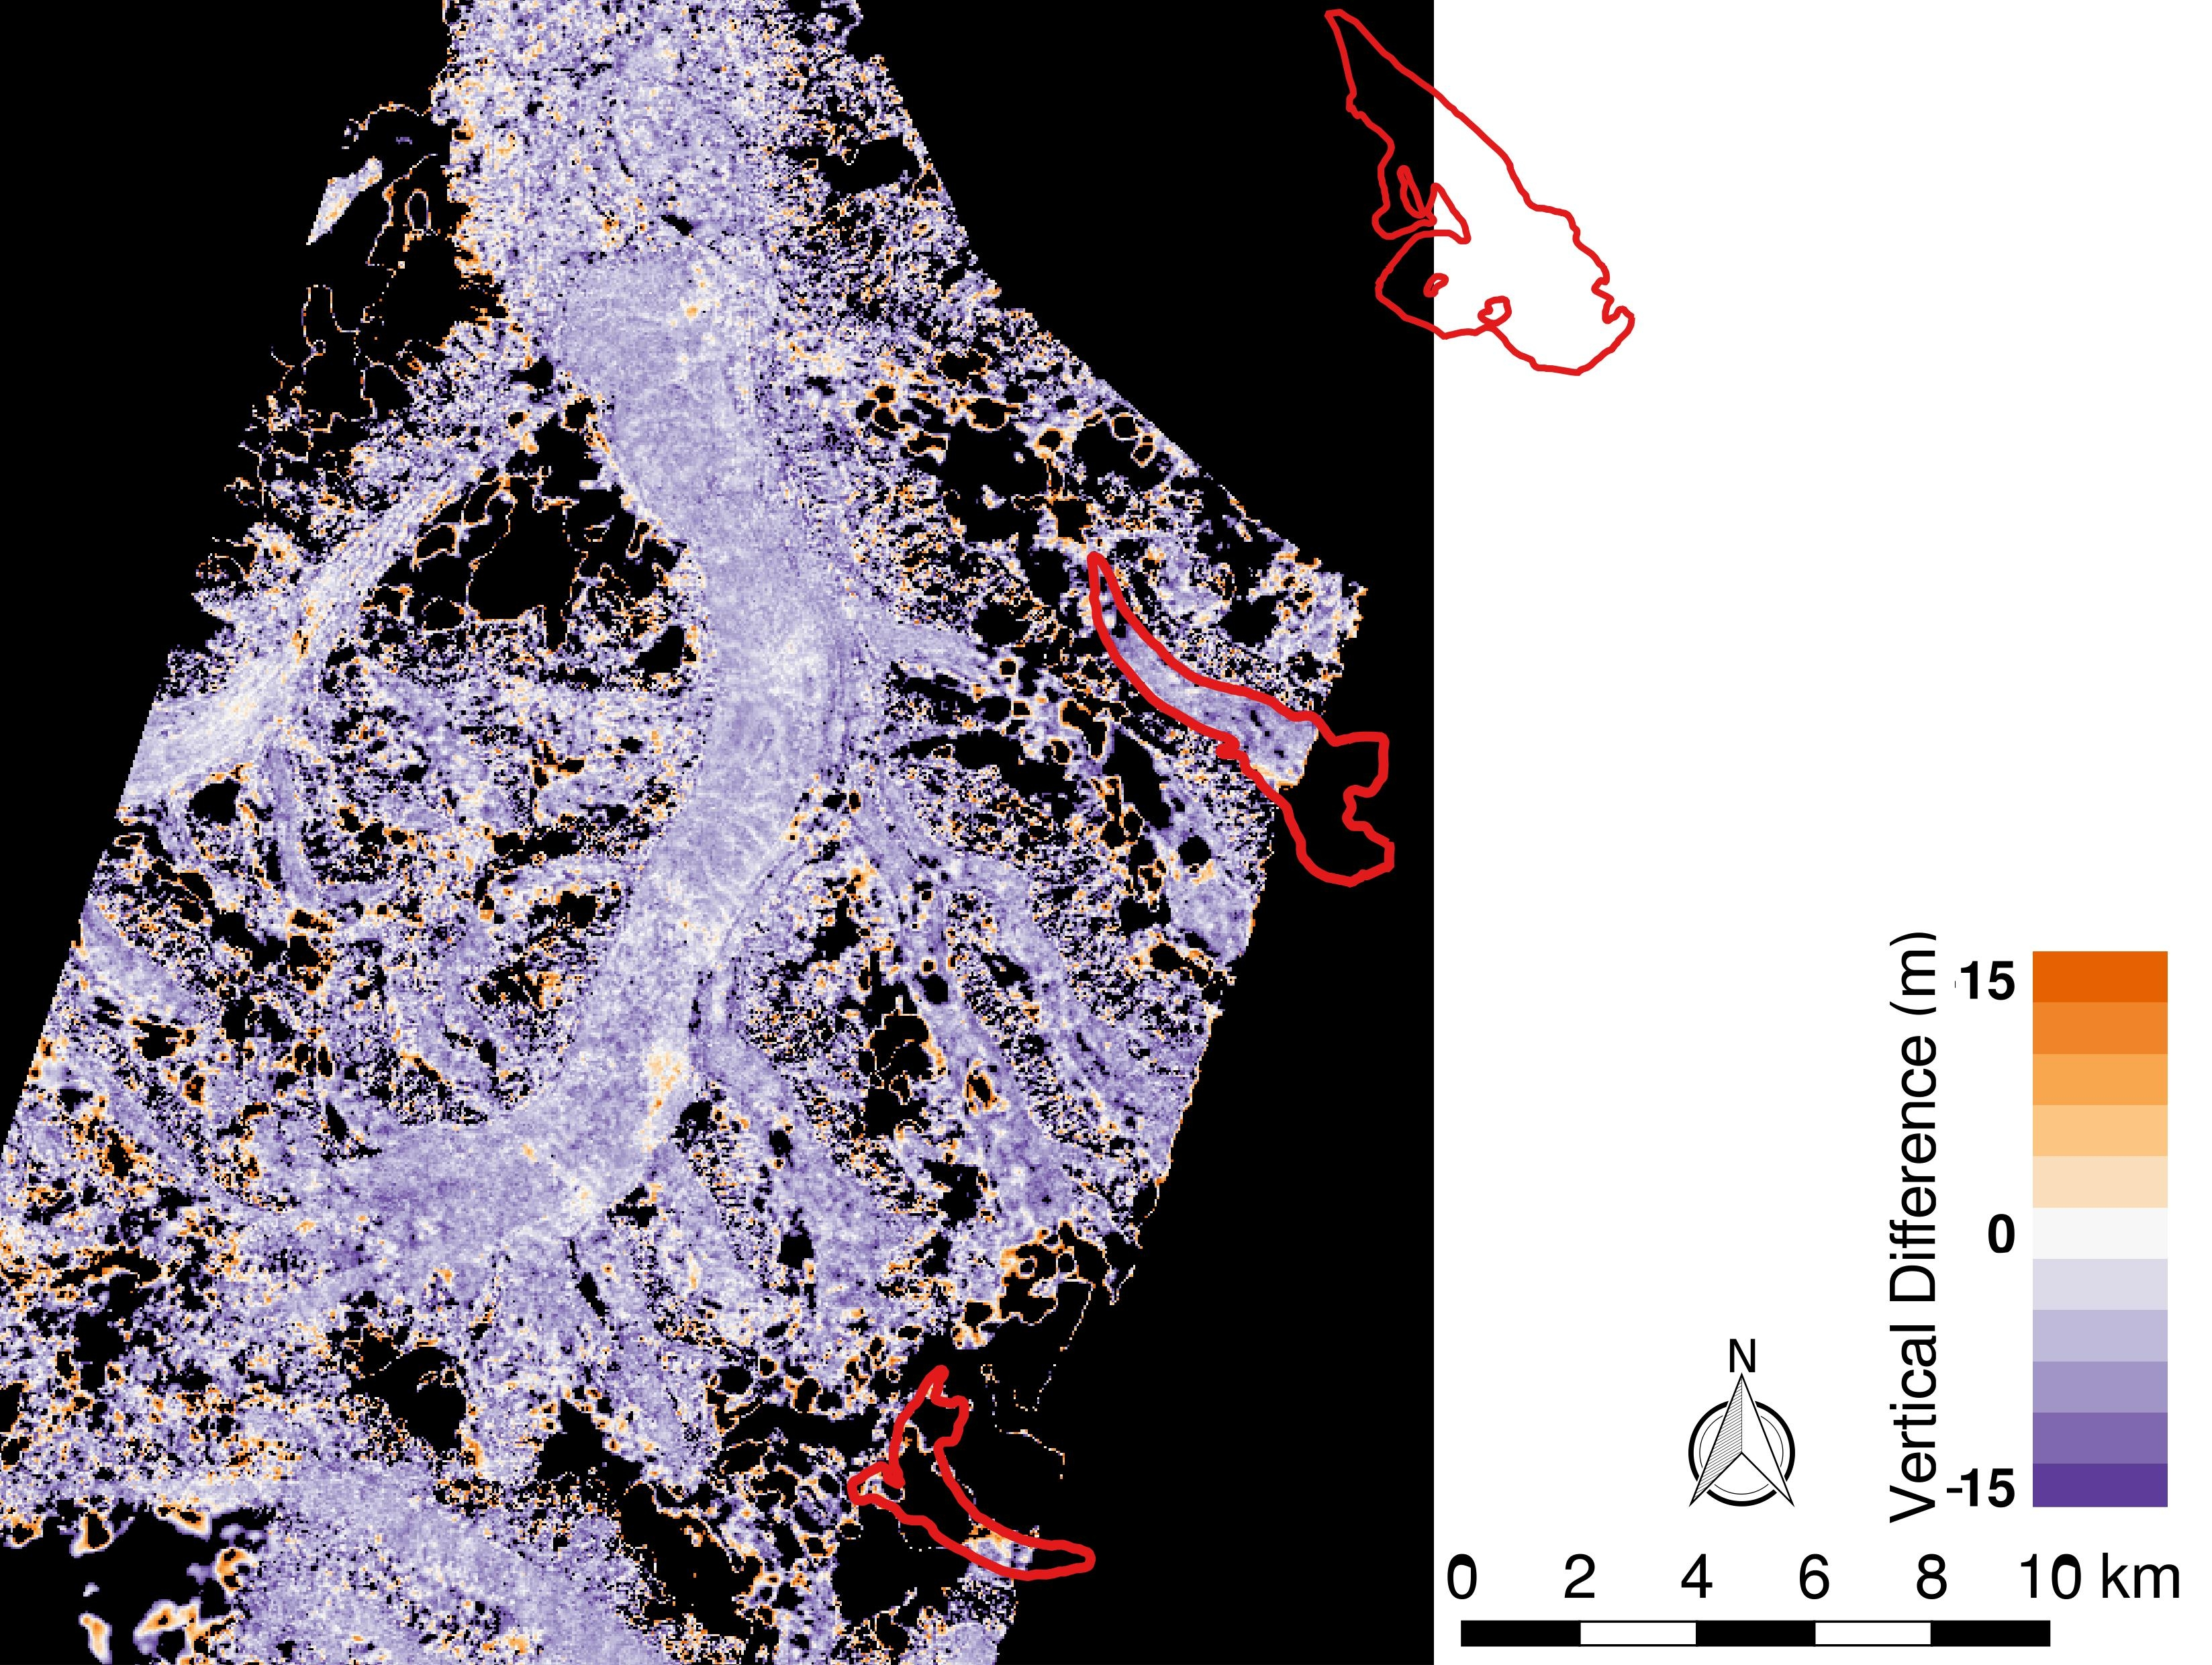
\includegraphics[width=\textwidth]{diff_7044-8029_original.jpeg}}
        \caption{Difference between original DEMs}
        \label{fig:DEMdifferenceOriginal}
    \end{subfigure}
    ~
    \begin{subfigure}[b]{0.48\textwidth}
        \fbox{\includegraphics[width=\textwidth]{diff_7044-8029_shift.jpeg}}
        \caption{Difference between corrected DEMs.}
        \label{fig:DEMdifferenceCorrected}
    \end{subfigure}

    \caption{Vertical difference between DEMs in overlapping area. Difference was found by subtracting GES 08-029 from GES 07-044. Positive values indicate that GES 07-044 values are higher than GES 08-029 values. }
 \label{fig:DEMdifference}
\end{figure}    
    
\begin{wrapfigure}{L}{0.6\textwidth}
	\centering
	\includegraphics[width = 0.6\textwidth]{DEMcorrection_hist.png}\\
	\caption{Histogram of the vertical difference between GES 08-029 and GES 07-044 before (dark blue) and after (light blue) correction. }
	\label{fig:DEMcorrection_hist}
\end{wrapfigure}    
    

The merging process was complicated by the fact that there was a horizontal discrepancy between the two DEMs. Although the discrepancy was not consistent throughout the study area, the GES 07-044 DEM was generally higher than the first, as can be seen by the overall purple colour in Figure \ref{fig:DEMdifferenceOriginal} and the positive skew of the vertical difference between the two DEMs in Figure \ref{fig:DEMcorrection_hist}. The mean vertical difference is +6.3 m.


\begin{wrapfigure}{R}{0.6\textwidth}
	\centering
	\includegraphics[width = 0.6\textwidth]{mergeLine.jpeg}\\
	\caption{Outlines of the cropped GES 07-044 DEM (pink, left) and cropped GES 08-029 DEM (blue, right) used for merging. There is a slight overlap between the two DEMs that cannot be seen at this scale.}
	\label{fig:mergeLine}
\end{wrapfigure}

The discrepancy was corrected by E. Bertier (2016, personal communication) using an iterative 3D-coregistration algorithm \citep{Berthier2007}. The GES 07-044 DEM was arbitrarily chosen to be used as the reference DEM. Note that the absolute value of the elevation is not necessarily important for the topographic regression, as long as the relative elevations are correct. The reference DEM (GES 07-044) was first shifted vertically by $+$5.4\,m, which was estimated using ICESat data \citep{Berthier2010}. Then, the mean horizontal and vertical (X, Y, Z) shift between the reference DEM and the GES 08-029 DEM was found by minimizing the standard deviation of the elevation differences between the DEMs. Using this correlation, the GES 08-029 DEM  was shifted $\sim$2\,m east, $\sim$4\,m north and $\sim$1.9\,m vertically. The GES 08-029 DEM was then reprojected in the same projection as the reference DEM (GES 07-044). The difference map between the two shifted DEMs is shown in Figure \ref{fig:DEMdifferenceCorrected}. Difference values are not uniform but do show both positive and negative values. The distribution of vertical difference values (Figure \ref{fig:DEMcorrection_hist}) after correction is centred at zero with a mean difference of $-$0.2\,m.

Merging of the corrected DEMs was completed in QGIS. First, the rasters were cropped to overlap by a few cells. The crop line was chosen by hand to include as much of the reference DEM as possible (Figure \ref{fig:mergeLine}). The second DEM was cropped to follow the same merge line but overlap with the first DEM by a few cells. This was done to avoid gaps in cell values that arise from cropping across a DEM cell. The merging was completed using the built in QGIS tool `Merge' and in areas where the two DEMs overlapped, the GES 08-029 DEM values were chosen.

The final DEM used for subsequent analysis can be seen in Figure 4. Despite the corrections, there were still discrepancies along the intersection of the DEMs, which can be seen as sharp boundaries in the contour lines. However, these discrepancies are more than 250\,m from the edge of any of the glaciers so this DEM was used as the final version for the Donjek Range.

\begin{figure}[H]
\begin{adjustbox}{addcode={\begin{minipage}{\width}}{\caption{%
      Merged DEM of the Donjek Range from two corrected SPOT-5 DEMs, plotted with 10\,m contour lines. Study glaciers are shown in red. Discrepancies between the DEMs along the merge line can be seen as anomalous linear features in the contour map (yellow boxes). Distorted contours in the eastern regions (white box) are a result of errors in the DEM. 
      }\end{minipage}},rotate=90,center}
     	\includegraphics[height = 0.9\textwidth]{mergedDEM2.jpeg}%
 \end{adjustbox}  
  \label{fig:finalDEM}
\end{figure}

\section{Topographic parameters}
\label{sec:topoCalc}

Topographic parameters are used to describe characteristics of the local landscape that may affect snow distribution and can act as proxies for physical processes that determine snow deposition and redistribution. Topographic parameters used in snow accumulation studies on glaciers include elevation ($z$), slope ($m$), tangential ($\kappa_T$) and profile ($\kappa_P$) curvature, northness ($N$), aspect ($\alpha$) and wind redistribution parameter ($Sx$) \citep{Basist1994, Revuelto2014, McGrath2015}.	We add distance from centreline ($d_C$) as an additional parameter.
 
A number of programs are used to calculate topographic parameters from the DEM. Distance from centreline and northness were calculated in Matlab. $Sx$ was determined using a executable obtained from Adam Winstral that follows the procedure outlined in \cite{Winstral2002}. The remaining parameters were calculated using the \texttt{r.slope.aspect} module in GRASS GIS software run through QGIS as described in \cite{Mitavsova1993} and \cite{Hofierka2009}. Note that topographic parameters were calculated using the full DEM and then trimmed to the glacier outlines as defined in the Randolph Glacier Inventory so as to avoid errors that arise at the edge of the DEM when taking derivatives. Note that the outlines defined by the Randolph Glacier Inventory were modified slightly to match the 2015 glacier outlines as seen in Landsat 7 imagery.

\subsection{Calculating topographic parameters}

Details about the calculation of topographic parameters are described below and a summary of topographic parameters is found in Table \ref{tab:TopoParams}.
\subsubsection*{Elevation}

Elevation ($z$) values were taken from the (corrected) SPOT-5 DEMs directly (Figure \ref{map:elev}).

\subsubsection*{Distance from centreline}

Distance from centreline ($d_C$) was calculated as the minimum distance between the Easting and Northing coordinates of the northwest corner of each cell and a manually defined centreline (Figure \ref{map:centreD}). 


\subsubsection*{Slope} 

Slope ($m$) is the maximal rate of change of elevation and is defined as the angle between a plane tangential to the surface (gradient) and the horizontal \citep{Olaya2009} (Figure \ref{map:slope}). Slope ($m$) is calculated according to 
\begin{equation}
m = \arctan \sqrt{\left( \frac{\partial z}{\partial x} \right) ^2 + \left( \frac{\partial z}{\partial y} \right) ^2},
\end{equation}
where the partial derivatives can be approximated by \citep{Mitavsova1993, Neteler2008, Hofierka2009}
\begin{align} \label{eq:firstpartial}
\frac{\partial z}{\partial x} &\approx \frac{(z_{i-1,j-1}-z_{i+1,j-1})+(2z_{i-1,j}-2z_{i+1,j})+(z_{i-1,j+1}-z_{i+1,j+1})}{8  \Delta x},\nonumber \\
\frac{\partial z}{\partial y} &\approx \frac{(z_{i-1,j-1}-z_{i-1,j+1})+(2z_{i,j-1}-2z_{i,j+1})+(z_{i+1,j-1}-z_{i+1,j+1})}{8  \Delta y}.
\end{align}
Here, $z_k$ refers to one of the gridcells surrounding the cell of interest, which is located at row $i$ and column $j$ of the DEM. The grid spacing (resolution) of the DEM is $\Delta x$ and $\Delta y$ in the east-west and north-south direction, respectively \citep{Neteler2008}. 

\subsubsection*{Aspect} 

Aspect ($\alpha$) represents the orientation of the steepest slope, with 0${^\circ}$ defined as North and no value given to cells that have zero slope. The equation for aspect is \citep{Neteler2008}
	\begin{equation}
	\alpha = \arctan\left(\frac{\partial z}{\partial y} \bigg/ \frac{\partial z}{\partial x}\right), 
	\end{equation}
where the partial derivatives are approximated by Equations \ref{eq:firstpartial}. Here, $\alpha = 0$ is west but the computed values are transformed such that 0${^\circ}$ is north (clockwise). 

Aspect is a circular parameter (0${^\circ}$ is the same as 360${^\circ}$) but regressions (Section \ref{sec:linearregression}) require that a parameter is linear. Therefore, only the sine of aspect was used in topographic analysis. The sine of aspect is a proxy for the relative amount of direct solar radiation incident on a slope.


\subsubsection*{Curvature} 

Curvature describes the convexity or concavity of a surface. The curvature of a surface is different in different directions, so curvature may be defined in various ways. Profile and tangential curvature are the most common types to consider in geophysical systems. For this study, the mean curvature ($\kappa$), found by taking the average of profile and tangential curvature, is used. Relative accumulation would be expected to occur in mean-concave (positive values) areas and relative scour would be expected to occur in and mean-convex (negative values) terrain \citep{Olaya2009}.

Profile curvature is the curvature in the direction of the surface gradient and it describes the change in slope angle. The equation for profile curvature ($\kappa_p \left[\mathrm{m}^{-1}\right]$) is \citep{Neteler2008}
\begin{equation} 
\kappa_p = \frac{\frac{\partial^2 z}{\partial x^2} \big(\frac{\partial z}{\partial x}\big)^2 + 2\frac{\partial^2 z}{\partial x \partial y}\frac{\partial z}{\partial x}\frac{\partial z}{\partial y} +  \frac{\partial^2 z}{\partial y^2} \big(\frac{\partial z}{\partial y}\big)^2}{\left[\big( \frac{\partial z}{\partial x} \big) ^2 + \big(\frac{\partial z}{\partial y} \big)^2\right] \sqrt{\left[\big(\frac{\partial z}{\partial x} \big) ^2 + \big( \frac{\partial z}{\partial y}\big) ^2+1\right]^3}}
\end{equation} 
where first-order partial derivatives are found using Equation \ref{eq:firstpartial}. Second-order partial derivatives can be approximated by \citep{Hofierka2009, Neteler2008}
\begin{align}\label{eq:secondpartial}
\frac{\partial^2 z}{\partial x^2} &\approx\frac{z_{i-1,j+1}-2z_{i,j+1}+z_{i+1,j+1}+4z_{i-1,j}-8z_{i,j}+4z_{i+1,j}+z_{i-1,j-1}-2z_{i,j-1}+z_{i+1,j-1}}{6  (\Delta x)^2},\nonumber\\
\frac{\partial^2 z}{\partial y^2} &\approx \frac{z_{i-1,j+1}-4z_{i,j+1}+z_{i+1,j+1}-2z_{i-1,j}-8z_{i,j}-2z_{i+1,j}+z_{i-1,j-1}+4z_{i,j-1}+z_{i+1,j-1}}{6  (\Delta y)^2},\nonumber\\
\frac{\partial^2 z}{\partial x \partial y} &\approx \frac{(z_{i-1,j-1}-z_{i+1,j-1})-(z_{i-1,j+1}-z_{i+1,j+1})}{4  \Delta x \Delta y}.
\end{align}
Tangential Curvature represents the curvature in the direction of the contour tangent. The equation for profile curvature ($\kappa_t \left[\mathrm{m}^{-1}\right]$) is \citep{Neteler2008}
\begin{equation}
\kappa_t = \frac{\frac{\partial^2 z}{\partial x^2} \big(\frac{\partial z}{\partial y}\big)^2 - 2\frac{\partial^2 z}{\partial x \partial y}\frac{\partial z}{\partial x}\frac{\partial z}{\partial y} +  \frac{\partial^2 z}{\partial y^2} \big(\frac{\partial z}{\partial x}\big)^2}{\left[\big( \frac{\partial z}{\partial x} \big) ^2 + \big(\frac{\partial z}{\partial y} \big)^2\right] \sqrt{\big(\frac{\partial z}{\partial x} \big) ^2 + \big( \frac{\partial z}{\partial y}\big) ^2 +1}},
\end{equation} 	
where first- and second-order partial derivatives are approximated using Equations \ref{eq:firstpartial} and \ref{eq:secondpartial}. 

\subsubsection*{Northness} 

``Northness'' ($N$) is a proxy parameter for solar radiation processes that affect accumulation distribution, especially during the spring \citep{Revuelto2014}. It is also been suggested that this parameter is related to sun-induced snow metamorphosis and/or sun crusts, both of which affect point-scale winter balance \citep{McGrath2015}. Northness is defined as 
\begin{equation}
N = \cos{\alpha} \times \sin{m},
\end{equation}
where $\alpha$ is aspect and $m$ is slope \citep{Molotch2005}. A value of $-$1 represents a vertical, south facing slope, a value of $+$1 represents a vertical, north facing slope and a flat surface yields 0. 


\subsubsection*{Wind redistribution parameter} 

$Sx$ represents wind exposure/shelter and requires the identification of a cell within a certain angle and distance from the cell of interest that has the greatest upward slope relative to the cell of interest \citep{Winstral2002}. The identified cell is referred to as the maximum upwind slope. Negative $Sx$ values represent exposure relative to the shelter-defining pixel, which means that the cell of interest is higher than the cell with greatest upwind slope. Conversely, positive values represent sheltered cells. To determine $Sx$ values, the following equation is used
\begin{equation}
Sx_{A, d\max}(x_i, y_i) = \textrm{max} \left[ \textrm{tan}^{-1} \left( \frac{z(x_v,y_v)-z(x_i,y_i)}{[(x_v-x_i)^2+(y_v-y_i)^2]^{1/2}} \right) \right] ,
\end{equation}
where A is the azimuth of the search direction, $(x_i, y_i)$ are the coordinates of the cell of interest and $(x_v, y_v)$ are the set of all cell coordinates located along the search vector defined by	$(x_i, y_i)$, the azimuth ($A$) and maximum search distance ($d$max). Code for this calculation was provided by Adam Winstral (2016, personal communication). As done by \cite{McGrath2015}, I compute $Sx$ at 5$^{\circ}$ azimuth increments for $d$max distances of 100, 200 and 300 m. These values are then correlated (Pearson correlation) with observed values of point-scale winter balance and the $Sx$ values from the combination of azimuth and $d$max input values that have the highest correlation are used for subsequent analysis (Table \ref{tab:Sxparams}). The code for calculating $Sx$ requires a UTM raster formatted to ASCII in ArcGIS. 



%% TOPO PARAMS TABLE
\begin{landscape}
\begin{table}
\footnotesize
\begin{threeparttable}
   %\captionsetup{singlelinechec\FloatBarrierk=off, skip=4pt}
\caption{Description of topographic parameters used in the linear regression.}
\label{tab:TopoParams}
\begin{tabularx}{22cm}{XXXXX}
\midrule
\textbf{\begin{tabular}[c]{@{}l@{}}Topographic\\ parameter\end{tabular}} & \textbf{Definition} & \textbf{\begin{tabular}[c]{@{}l@{}}Calculation \\ method\end{tabular}} & \textbf{Notes} & \textbf{Source} \\ \midrule
\textbf{Elevation ($z$)} & Height above sea level & Values taken directly from DEM &  &  \\ \midrule
\textbf{Distance from centreline ($d_C$)} & Linear distance from user-defined glacier centreline & Minimum distance between the Easting and Northing of the northwest corner of each gridcell and a manually defined centreline &  &  \\ \midrule
\textbf{Slope ($m$)} & Angle between a plane tangential to the surface (gradient) and the horizontal & \texttt{r.slope.aspect} module in GRASS GIS software run through QGIS &  & \cite{Mitavsova1993, Hofierka2009, Olaya2009} \\ \midrule
\textbf{Aspect ($\alpha$)} & Dip direction of the slope & \texttt{r.slope.aspect} module in GRASS GIS software run through QGIS & $\sin(\alpha)$, a linear quantity describing a slope as north/south facing, is used in the regression & \cite{Mitavsova1993, Hofierka2009, Olaya2009} \\ \midrule
\textbf{Mean curvature ($\kappa$)} & Average of profile (direction of the surface gradient) and tangential (direction of the contour tangent) curvature & \texttt{r.slope.aspect} module in GRASS GIS software run through QGIS & ($+$) mean-concave terrain and ($-$) mean-convex terrain & \cite{Mitavsova1993, Hofierka2009, Olaya2009} \\ \midrule
\textbf{Northness ($N$)} & A value of $-1$ represents a vertical, south facing slope, a value of $+1$ represents a vertical, north facing slope and a flat surface yields 0 & Product of the cosine of aspect and sine of slope &  & \citep{Molotch2005} \\ \midrule
\textbf{Wind redistribution parameter ($Sx$)} & Proxy for snow deposition due to wind redistribution & Executable obtained from Adam Winstral that follows the procedure outlined in \cite{Winstral2002} & Calculation based on selecting a cell within a certain angle and distance from the cell of interest that has the greatest upward slope relative to the cell of interest & \citep{Winstral2002}
\end{tabularx}
\end{threeparttable}
\end{table}
\end{landscape}


\begin{figure}[H]
	\centering
	\includegraphics[width = 0.6\textwidth]{Sx_infographic.jpeg}\\
	\caption{ Example of $Sx$ calculations for three cells of interest along a 270$^\circ$ search vector. As depicted, with $d$max set equal to 300 m, the shelter-defining cell for cells 1 and 2 is cell A, producing positive $Sx$ values. The shelter-defining cell for cell 3 is cell B, producing a negative $Sx$. Had $d$max been equal to 100\,m, the search for the shelter-defining  cell  for  cell  1  would  not  extend  across  the  valley,  thus producing a negative $Sx$ for cell 1, while $Sx$ for cell 2 would remain the same and that for cell 3 would be slightly lower. Image and description from \citep{Winstral2002}.}
	\label{fig:Sx_infographic}
\end{figure}


\begin{table}
\centering
\caption{Values of azimuth ($A$) and maximum search distance ($d$max), that correspond to the $Sx$ that had the highest absolute correlation to observed WB.}
\label{tab:Sxparams}
\begin{tabular}{lccc}
 & \begin{tabular}[c]{@{}c@{}}$A$\\ ($^{\circ}$ from North)\end{tabular} & \begin{tabular}[c]{@{}c@{}}$d$max \\ (m)\end{tabular} & \begin{tabular}[c]{@{}c@{}}Correlation\\ Coefficient\end{tabular} \\ \hline
Glacier 4 & 85 & 300 & $-$0.26 \\
Glacier 2 & 330 & 300 & 0.56 \\
Glacier 13 & 280 & 200 & 0.28
\end{tabular}
\end{table} 

\subsection{DEM smoothing}

Visual inspection of the curvature fields calculated using the DEM indicated that the spatial patterns of curvature were noisy and did not vary smoothly. \cite{Olaya2009} states that the curvature calculation is sensitive to noisy data and a smoothing filter must often be applied to the DEM prior to calculation. Curvature, as well as slope, aspect and northness, are all sensitive to noise because calculating these parameters involves calculating the first and second derivatives of the elevation which are highly dependent on the size of the DEM cell. To minimize the effect of noise on these four parameters, a smoothing filter was applied to the DEM and this smoothed DEM was used to calculate curvature, slope, aspect and northness. The unsmoothed DEM was used to determine elevation and $Sx$ because these parameters do not depend on a topographic length scale and their values are not as sensitive to the size of the DEM gridcell.

To choose a smoothing algorithm and window size, I applied a number of smoothing algorithms and chose the combination that resulted in the highest correlation between topographic parameters and point-scale winter balance values. Window sizes of 3$\times$3, 5$\times$5, 7$\times$7 and 9$\times$9 gridcells were used. For all sizes, inverse-distance weighted smoothing and Gaussian smoothing were poorly correlated with WB. The smoothing algorithm that used 7$\times$7 window resulted in the highest correlation between curvature (second derivative) and WB as well as slope (first derivative) and WB. The window size that produced the highest correlation of WB values and curvature for each glacier differed, but for all WB values taken together, the 7$\times$7 window resulted in the highest correlation. For slope, all three glaciers showed highest correlation with 7$\times$7 smoothing window, but not when combined. To maintain consistency between parameters, the 7$\times$7 smoothing window was chosen and applied to the DEM for calculation of curvature, slope, aspect and northness. 

\begin{figure}[H]
	\centering
	\includegraphics[width = 0.7\textwidth]{G13curvatureSmoothing.jpeg}\\
	\caption{(a) Curvature found using the original DEM. (b) 
	Curvature found using the smoothed (7$\times$7 window moving average) DEM.}
	\label{fig:smoothingCurve}
\end{figure}


\subsection{Parameter correlations}

The correlation between topographic parameters at sampling locations on each glacier is shown in Table \ref{tab:pearson_correlation}. Correlation values are generally low, with the exception of the correlation between northness and aspect on Glacier 2 and northness and $Sx$ on Glacier 13 which were both larger than 0.7. Since there is little correlation between parameters and the correlations vary between glaciers, the use of a linear regression with these topographic parameters as predictor variables is warranted. 

\begin{table}[H]
\centering
\caption{Pearson correlation coefficients between topographic parameters at snow-depth sampling locations. \params}
\label{tab:pearson_correlation}
\begin{tabular}{cc|ccccccc}
 &  & $z$ & $d_C$ & $\alpha$ & $m$ & $N$ & $\kappa$ & $Sx$ \\ \hline
\multirow{7}{*}{Glacier 4} & $z$ & 1 & 0.16 & $-$0.57 & $-$0.08 & $-$0.51 & 0.17 & 0.43 \\
 & $d_C$ &  & 1 & 0.13 & 0.56 & 0.16 & $-$0.43 & 0.35 \\
 & $\alpha$ &   &  & 1 & 0.57 & 0.95 & $-$0.61 & $-$0.58 \\
 & $m$ &   &   &   & 1 & 0.64 & $-$0.58 & $-$0.10 \\
 & $N$ &   &   &   &   & 1 & $-$0.59 & $-$0.59 \\
 & $\kappa$ &   &   &   &   &   & 1 & 0.05 \\
 & $Sx$ &   &   &   &   &   &   & 1 \\ \hline
\multirow{7}{*}{Glacier 2} & $z$ & 1 & 0.06 & $-$0.52 & $-$0.58 & $-$0.62 & 0.45 & 0.57 \\
 & $d_C$ &   & 1 & 0.06 & 0.13 & 0.11 & $-$0.27 & 0.01 \\
 & $\alpha$ &   &  & 1 & 0.33 & 0.86 & $-$0.42 & $-$0.45 \\
 & $m$ &   &   &   & 1 & 0.74 & $-$0.67 & $-$0.41 \\
 & $N$ &   &   &   &   & 1 & $-$0.67 & $-$0.48 \\
 & $\kappa$ & &   &   &   &   & 1 & 0.28 \\
 & $Sx$ &   &   &   &   &   &   & 1 \\ \hline
\multirow{7}{*}{Glacier 13} & $z$ & 1 & 0.15 & 0.19 & $-$0.15 & 0.10 & 0.02 & 0.27 \\
 & $d_C$ &   & 1 & $-$0.05 & 0.18 & 0.10 & $-$0.45 & 0.06 \\
 & $\alpha$ &   &   & 1 & $-$0.07 & 0.68 & $<$0.01 & 0.45 \\
 & $m$ &   &   &   & 1 & 0.63 & $-$0.22 & $-$0.22 \\
 & $N$ &   &   &   &   & 1 & $-$0.21 & 0.23 \\
 & $\kappa$ &   &   &   &   &   & 1 & $-$0.30 \\
 & $Sx$ &   &   &   &   &   &   & 1
\end{tabular}
\end{table}


\subsection{Topographic parameter distributions}


Elevation maps (Figure \ref{map:elev}) show that high elevation area on both Glacier 2 and 13 are confined to steep headwalls. Mean elevation is within one standard deviation for all glaciers for the full and sampled distribution (Table \ref{tab:sampled&fullParams_stats}). However, maximum elevation values are lower for Glacier 4 than the other two glaciers (Figure \ref{sampledRange:elev}) and the sampled elevation means are approximately 200\,m less than that of the full distribution. Standard deviations are smaller for sampled ranges for all glaciers. The skewness of sampled and full distributions is different for all glaciers. Full distributions of elevation are similar for the study glaciers, with kurtosis for all distributions, except sampled elevation on Glacier 13, being less than 3 (value for a normal distribution). Kurtosis of sampled distributions shows that Glacier 13 has a broader distribution and Glacier 2 has a narrower distribution. 

The mean of sampled distance from centreline (Figure \ref{sampledRange:centreD}) is different from that of the full distribution for all glaciers (Table \ref{tab:sampled&fullParams_stats}). Large values of distance from centreline are located at the edges of the glacier in the accumulation area (Figure \ref{map:centreD}), which constitute steep, inaccessible terrain. Within the ablation area, the hourglass sampling pattern allowed for locations across the whole width of the glacier to be measured. Note that Glacier 13 has two centrelines in the accumulation area because of the confluence of two major arms of the glacier.

The aspect of Glaciers 2 and 13 indicate that most of the glacier area is north facing, while most of Glacier 4 is south facing (Figure \ref{map:aspect}). This is also highlighted in the mean values of aspect, which are positive for Glaciers 2 and 13 and negative for Glacier 4 (Table \ref{tab:sampled&fullParams_stats}). Sampled mean aspect is similar to the full distribution, although the standard deviation of sampled aspects is much lower. Further, the skewness and kurtosis of the sampled distributions differ considerably from the full distribution and there are many aspects that were not sampled (Figure \ref{sampledRange:aspect}). 

Slope of the three study glaciers (Figure \ref{map:slope}) is generally less than 20$^{\circ}$, with only the margins of the accumulation area and a few steps on Glacier 13 having steep slopes. The full and sampled distributions of slope are similar between glaciers (Table \ref{tab:sampled&fullParams_stats}), with mean values of $\sim$13$^{\circ}$ for the full distribution and 5$^{\circ}$ to 8$^{\circ}$ for the sampled distribution. The sampled distributions are all different than the full range, as indicated by the lower means, standard deviations and skewness, as well as larger kurtosis. The sampled distributions severely under-represent steep slopes (Figure \ref{sampledRange:slope}).

The mean northness values for all glaciers is close to zero and the majority of cells have values close to zero, which is likely due to their low slope values (Figure \ref{map:northness}). Even for Glacier 4, which is largely south facing and should thus have lower values of northness, has a distribution with a mean close to zero (Table \ref{tab:sampled&fullParams_stats}). The low slope values mean that the values of northness were determined largely by the aspect, which can be seen by the resemblance between the northness map and the aspect map and their high correlation (Table \ref{tab:pearson_correlation}). Sampled distributions of northness do not resemble the full distributions. Although the mean values are similar, the skewness and kurtosis values are higher for all glaciers, indicating that the sampling is biased.

Curvature values on all glaciers are largely negative, indicating that concave topography is more prevalent than convex topography (Figures \ref{map:curvature} and \ref{sampledRange:curvature}). The sampled distribution of curvature is a poor representation of the full distribution as shown by the dramatically different values of skewness, which are positive for the full distribution and negative for the sampled distribution (Table \ref{tab:sampled&fullParams_stats}). 

$Sx$ maps over the study glaciers are shown in Figure \ref{map:Sx} and the wind direction and maximum search distance with the highest correlation to point-scale winter balance for each glacier are shown in Table \ref{tab:Sxparams}. For Glacier 4, an approximately east wind and 300 m search distance were most strongly correlated. The correlation was negative, which means that negative values of $Sx$ (exposure) correspond to areas with higher winter balance (more snow). This is counter intuitive and perhaps indicates that $Sx$ is not an appropriate topographic parameter to correlate with WB on Glacier 4. Despite this, $Sx$ was retained in future analysis for consistency between glaciers. For Glacier 2, a north wind with a 300 m search distance was most strongly correlated and for Glacier 13, a west wind with a 200 m search distance produced the strongest correlation. Both of these correlations were positive, so a more positive $Sx$ value (sheltered) corresponds to higher values of point-scale winter balance (more snow). The correlation values for Glacier 4 and 2 are low ($<$0.3) which indicates that $Sx$ will likely be insignificant in estimating snow accumulation. The correlation between $Sx$ and point-scale winter balance on Glacier 2 is higher (0.56). 

The full distribution of $Sx$ (Figure \ref{sampledRange:Sx}) is different for each glacier and differs greatly between sampled and full distributions. Glacier 2 has a mean less than zero, indicating that a large portion of the glacier has exposed topography (Table \ref{tab:sampled&fullParams_stats}). Glacier 4 and 13 have positive mean values of $Sx$, indicating more sheltered topography. Extreme values of $Sx$ are generally located along the edges of the accumulation areas (Figure \ref{map:Sx}). The sampled distribution mean for Glacier 2 is close to that of its full distribution, while the sampled distribution means of Glacier 4 and 13 are different (negative) than that of the full distribution means (positive). The sampled distribution are more sharply peaked, as indicated by the smaller standard deviation values and larger kurtosis when compared to the full distributions. The skewness also differs for Glaciers 4 and 2, with the sampled distributions skewed more to the right than full distributions. Overall, the sampled distribution of $Sx$ is a poor representation of the full distribution. 

Overall, the sampled topographic parameters are poor representatives of the full distribution of parameters. Extreme values of all parameters are grossly under sampled and the distribution of the sampled parameters generally differs from the full distribution. This was largely do to dangerous travel conditions and an inability to quickly and accurately measure snow depth in the accumulation area. As a result, extrapolation of regression models will likely result in large errors. These errors are especially relevant in the accumulation area, which has extreme values for all parameters. Errors in the accumulation area are especially important to acknowledge because this area has the highest winter balance values and is likely to heavily influence glacier-wide winter balance values. Generally, the sampled values do not fully capture the variance in topographic parameters but a regression is still valuable  since topographic regressions are common when estimating winter balance.  

\begin{sidewaystable}
\small
\centering
\caption{Descriptive statics of topographic parameter full and sampled distribution. Mean and standard deviation are in units of meters for distance from centreline ($d_C$) and elevation ($z$), in units of m$^{-1}$ for profile ($\kappa_P$) and tangential ($\kappa_T$) curvature and are unitless for cosine of aspect ($\alpha$), northness ($N$), slope ($m$) and wind redistribution ($Sx$). Skewness is a measure of the data asymmetry about the mean, with positive values indicating data that are more spread to the right of the mean and zero indicating a perfectly symmetric distribution. Kurtosis is a measure of how prone a distribution is to outliers. A normal distribution has a kurtosis value of 3 and larger values indicate distributions that are more prone to outliers.}
\label{tab:sampled&fullParams_stats}
\begin{tabular}{cc|cccc|cccc}
 & \textbf{} & \multicolumn{4}{c|}{\textbf{Full}} & \multicolumn{4}{c}{\textbf{Sampled}} \\
\textit{\textbf{}} & \textit{} & \textit{Mean} & \textit{\begin{tabular}[c]{@{}c@{}}Standard \\ Deviation\end{tabular}} & \textit{Skewness} & \textit{Kurtosis} & \textit{Mean} & \textit{\begin{tabular}[c]{@{}c@{}}Standard \\ Deviation\end{tabular}} & \textit{Skewness} & \textit{Kurtosis} \\ \hline
\multirow{7}{*}{\textbf{Glacier 4}} & $z$ & 2343.76 & 178.36 & $-$0.17 & 2.13 & 2242.63 & 89.52 & 0.00 & 2.59 \\
 & $d_C$ & 258.95 & 233.49 & 1.82 & 6.52 & 124.33 & 89.56 & 0.32 & 2.04 \\
 & $\alpha$ & $-$0.35 & 0.61 & 0.75 & 2.23 & $-$0.37 & 0.53 & 0.85 & 2.57 \\
 & $m$ & 12.81 & 7.03 & 1.11 & 3.37 & 8.32 & 3.17 & 2.19 & 8.10 \\
 & $N$ & $-$0.05 & 0.17 & 0.52 & 4.04 & $-$0.04 & 0.10 & 1.35 & 5.04 \\
 & $\kappa$ & $-$53.32 & 70.30 & 0.76 & 7.81 & $-$33.34 & 38.33 & $-$0.80 & 2.95 \\
 & $Sx$ & 1.56 & 11.46 & 1.03 & 4.28 & $-$1.06 & 5.17 & 1.62 & 6.21 \\ \hline
\multirow{7}{*}{\textbf{Glacier 2}} & $z$ & 2494.71 & 233.03 & 0.09 & 2.82 & 2306.90 & 93.74 & $-$0.02 & 1.93 \\
 & $d_C$ & 304.95 & 236.97 & 1.22 & 4.51 & 140.65 & 98.84 & 0.37 & 2.74 \\
 & $\alpha$ & 0.59 & 0.43 & $-$1.43 & 4.83 & 0.52 & 0.33 & $-$0.42 & 2.14 \\
 & $m$ & 13.02 & 9.48 & 1.08 & 3.00 & 6.54 & 2.24 & 1.97 & 9.12 \\
 & $N$ & 0.14 & 0.16 & 0.74 & 3.68 & 0.06 & 0.05 & 1.01 & 4.10 \\
 & $\kappa$ & $-$18.40 & 91.35 & 1.30 & 6.83 & $-$22.94 & 43.91 & $-$1.44 & 4.75 \\
 & $Sx$ & $-$3.82 & 9.34 & $-$0.18 & 6.09 & $-$3.63 & 2.59 & 0.81 & 4.81 \\ \hline
\multirow{7}{*}{\textbf{Glacier 13}} & $z$ & 2427.62 & 225.15 & 0.13 & 2.45 & 2219.45 & 82.25 & 0.92 & 5.67 \\
 & $d_C$ & 443.88 & 308.48 & 0.76 & 3.21 & 181.91 & 152.29 & 0.46 & 2.33 \\
 & $\alpha$ & 0.55 & 0.49 & $-$1.30 & 3.89 & 0.69 & 0.28 & $-$1.31 & 4.91 \\
 & $m$ & 13.36 & 10.13 & 1.15 & 3.51 & 5.10 & 1.98 & 2.20 & 12.99 \\
 & $N$ & 0.13 & 0.18 & 1.01 & 4.02 & 0.06 & 0.04 & 1.58 & 9.63 \\
 & $\kappa$ & $-$13.31 & 89.16 & 1.24 & 6.65 & $-$6.93 & 32.44 & $-$0.77 & 4.51 \\
 & $Sx$ & 3.69 & 12.08 & 0.97 & 3.68 & $-$1.62 & 3.94 & 0.90 & 4.95
\end{tabular}
\end{sidewaystable}

\pagebreak
\begin{figure}[H]
	\centering
	\includegraphics[width = \textwidth]{Map_elevation.png}\\
	\caption{Distributions of elevation ($z$) used in the topographic regressions for the study glaciers. This DEM is derived from a SPOT5 satellite image and has a grid size of 40$\times$40 m. Subsequent topographic parameters were derived from this DEM. \topomap}
	\label{map:elev}
\end{figure}

\begin{figure}[H]
  \makebox[\textwidth][c]{\includegraphics[width=1.2\textwidth]{SampledRangeTopo_elevation.png}}%
	\caption{Histograms of elevation ($z$) sampled (black) as compared to total range of elevation (white) of study glaciers.}
	\label{sampledRange:elev}
\end{figure}

\begin{figure}[H]
	\centering
	\includegraphics[width=\textwidth]{Map_centreD.png}\\
	\caption{Distributions of distance from centreline ($d_C$) used in the topographic regressions for the study glaciers. Centreline was drawn by hand in QGIS. \topomap}
	\label{map:centreD}
\end{figure}

\begin{figure}[H]
	 \makebox[\textwidth][c]{\includegraphics[width=1.2\textwidth]{SampledRangeTopo_centreD.png}}%
	\caption{Histograms of distance from centreline ($d_c$) sampled (black) as compared to total range (white) of distance from centreline of study glaciers.}
	\label{sampledRange:centreD}
\end{figure}

\begin{figure}[H]
	\centering
	\includegraphics[width=\textwidth]{Map_aspect.png}\\
	\caption{Distributions of the sine of aspect ($\alpha$), which indicates north-south component of a slope (+1 defined as north), used in the topographic regressions for the study glaciers. Values are derived from a smoothed DEM. \topomap}
	\label{map:aspect}
\end{figure}

\begin{figure}[H]
	 \makebox[\textwidth][c]{\includegraphics[width=1.2\textwidth]{SampledRangeTopo_aspect.png}}%
	\caption{Histograms of aspect ($\alpha$) sampled (black) as compared to total range (white) of aspect of study glaciers.}
	\label{sampledRange:aspect}
\end{figure}

\begin{figure}[H]
	\centering
	\includegraphics[width=\textwidth]{Map_slope.png}\\
	\caption{Distributions of slope ($m$) used in the topographic regressions for the study glaciers. Values were derived from a smoothed DEM (grid size of 40$\times$40 m) in QGIS. \topomap}
	\label{map:slope}
\end{figure}

\begin{figure}[H]
	 \makebox[\textwidth][c]{\includegraphics[width=1.2\textwidth]{SampledRangeTopo_slope.png}}%
	\caption{Histograms of slope ($m$) sampled (black) as compared to total range (white) of slope of study glaciers.}
	\label{sampledRange:slope}
\end{figure}

\begin{figure}[H]
	\centering
	\includegraphics[width=\textwidth]{Map_northness.png}\\
	\caption{Distributions of northness ($N$) used in the topographic regressions for the study glaciers. Northness is defined as the product of the cosine of aspect and sine of slope. A value of -1 represents a steep, south facing slope, a value of +1 represents a steep, north facing slope and flat surfaces yield 0. Values were derived from a smoothed DEM (grid size of 40$\times$40 m) in QGIS. \topomap}
	\label{map:northness}
\end{figure}

\begin{figure}[H]
	 \makebox[\textwidth][c]{\includegraphics[width=1.2\textwidth]{SampledRangeTopo_northness.png}}%
	\caption{Histograms of northness ($N$) sampled (black) as compared to total range (white) of northness of study glaciers.}
	\label{sampledRange:northness}
\end{figure}

\begin{figure}[H]
	\centering
	\includegraphics[width=\textwidth]{Map_curvature.png}\\
	\caption{Distributions of curvature ($\kappa$) used in the topographic regressions for the study glaciers. Values were derived from a smoothed DEM (grid size of 40$\times$40 m) in QGIS. Colour axis has been scaled to better resolve values close to zero. \topomap}
	\label{map:curvature}
\end{figure}

\begin{figure}[H]
	 \makebox[\textwidth][c]{\includegraphics[width=1.2\textwidth]{SampledRangeTopo_curvature.png}}%
	\caption{Histograms of curvature ($\kappa$) sampled (black) as compared to total range (white) of profile curvature of study glaciers.}
	\label{sampledRange:curvature}
\end{figure}

\begin{figure}[H]
	\centering
	\includegraphics[width=\textwidth]{Map_Sx.png}\\
	\caption{Distributions of $Sx$, which is a wind redistribution parameter, used in the topographic regressions for the study glaciers. See Section \ref{sec:topoCalc} and the original paper by \cite{Winstral2002} for more details on calculation. See Table \ref{tab:Sxparams} for values of best correlated azimuth and maximum search distance for each glacier. \topomap }
	\label{map:Sx}
\end{figure}

\begin{figure}[H]
	 \makebox[\textwidth][c]{\includegraphics[width=1.2\textwidth]{SampledRangeTopo_Sx.png}}%
	\caption{Histograms of $Sx$ sampled (black) as compared to total range (white) of $Sx$ of study glaciers.}
	\label{sampledRange:Sx}
\end{figure}


\section{Summary}

This chapter documents the process of obtaining topographic parameters, which include elevation, slope, curvature, distance from centreline, aspect, northness and wind redistribution, from a given DEM of the study area. Maps of each topographic parameter, as well as distributions of sampled and total values are shown. Processing steps, which include DEM corrections and stitching are also described. I find that a smoothing algorithm that takes the mean value of 7$\times$7 gridcells results in the highest correlation between curvature and WB data. The smoothed DEM is used for further analysis. 



%%%%%%%%%%%%%%%%%%%%%%%%%%%%%%%%%%
%%%%%% INTERPOLATION%%%%%%%%%%%%%%%%%%%%%%%%%%%%
\chapter{Interpolation}

To obtain a distributed estimate of winter balance (WB), gridcell-scale winter balance values need to be interpolated and extrapolated. Linear regression (LR), simple kriging (SK) and regression kriging (RK) are used to interpolate data. Linear regression (Section \ref{sec:linearregression}) relates gridcell-averaged WB and various topographic parameters. This method is simple and has precedent for success \citep[e.g.][]{McGrath2015}. Instead of a basic regression however, cross-validation and model averaging are used to test all combinations of the topographic parameters. The results from regression analysis are compared with simple kriging (SK) (Section \ref{sec:kriging}), a data-driven interpolation method free of any physical interpretation \citep[e.g.][]{Hock1999}. The two methods are then combined by kriging the residuals of the LR and adding them to the LR interpolation, a method known as regression kriging (Section \ref{sec:regressionkriging}). In Section \ref{sec:compareInterpMethods} the distributed WB estimates found using these three methods are compared.

%%%%%%%%%%%%%%%%%%%%%%%%%%%%%%%%%%%%%%%%%%%%%%%%%%
\section{Linear topographic regressions}
\label{sec:linearregression}

\subsection{Background}
Relating WB values and terrain parameters to better predict distributed WB within a basin has been employed for decades \citep[e.g.][]{Woo1978, Molotch2005, McGrath2015}. The most common type of relation between topographic parameters and WB is a linear regression, where the observed WB is related to a linear combination of topographic parameters at each measurement location. 

A linear regression takes the form
\begin{equation}
\vector{y} = \vector{X} \bm{\beta} + \bm{\varepsilon},
\end{equation}
where the matrix $\vector{X}$ contains the set of independent regressors $\vector{x}_i$ used to explain the dependant variable $\vector{y}$ \citep[e.g.][]{Davis1986}. The regression coefficient for each regressor is given by $\bm{\beta}$ and the error of the system is given by $\bm{\varepsilon}$. In my work, the matrix of independent regressors ($\vector{X}$) contains the topographic parameters at the sampling locations, the dependent variable $\vector{y}$ contains the gridcell-averaged values of WB and the $\bm{\beta}$ values are determined using a fitting model. While there are many types of fitting models, the ones employed in this study are multiple linear regression (MLR) and Bayesian model averaging (BMA).

To prevent over fitting of the data, regressions are calculated using cross validation. This means that for each regression, a randomly selected portion of the data is used to estimate regression coefficients and the coefficients are used to predict values that correspond to the remaining data \citep{Kohavi1995}. The root mean squared error (RMSE) between the estimated and observed data is then calculated. This process is repeated 1000 times and the regression coefficients that result in the lowest RMSE are then chosen for that model. 

We use model averaging to account for uncertainty when selecting predictors and to maximize the model's predictive ability \citep{Madigan1994}. The total number of models is $2^n$ , where $n$ is the number of topographic parameters. Seven topographic parameters are used, resulting in $2^7 = 128$ models. Model averaging is then used to determine the final regression coefficients. Model averaging is described in more detail for multiple linear regressions (MLRs) in Section \ref{sec:MLR} and for Bayesian Model Averaging (BMA) in Section \ref{sec:BMS}.

Once $\bm{\beta}$ values have been estimated, they can then be used to predict values of the dependent variable in other locations where regressors are known \citep{Davis1986}. For each gridcell, known values of topographic parameters can be multiplied by their respective $\bm{\beta}$ coefficients and added together to obtain the modelled or predicted value of WB.

\subsection{Importance of variables in regression models}

Regressions are used not only for estimating the response variable but also for assessing the relative importance of the regressors. Most types of regression models, including the ones used in this study, cannot be used to directly determine variable importance, so many additional metrics have been developed to address this need. \cite{Gromping2015} lists seven simple metrics for assessing variable importance in a univariate regression (one dependant variable). Two of these metrics, raw correlation and semi-partial correlation, are chosen for this study. For both metrics, a larger value indicates a larger influence of a regressor in the model.

The first metric is the square of the raw correlations between regressors and response variable \citep{Gromping2015}. Raw correlation values can aid in identifying important variables for explaining and interpreting results because it is ignorant of which other regressors are included in the model \citep{Darlington1968}. 

The second metric is the square of the semi-partial (or part) correlations for each regressor variable \citep{Gromping2015}. Semi-partial correlations are the correlation between the response variable and the residuals of the regression between each regressor and the remaining regressors. The value can be interprested as the unique variance accounted for by $\vector{x}_1$ in the presence of other predictors $\vector{x}_2,...,\vector{x}_\mathrm{k}$ \citep{Darlington1968, Bring1996}. Semi-partial correlations are helpful in identifying a small number of regressors that have the most influence in the regression \citep{Gromping2009}. An assumption for semi-partial correlation is that regressors are independent of each other. When regressors are independent, the semi-partial correlations of all regressors sum to the total coefficient of determination (R$^2$) of the regression  \citep{Gromping2015}. In this study, the regressors are all independent (R$^2<$0.35 for all glaciers) except for aspect and northness, which have R$^2$ values of 0.79, 0.83 and 0.64 for Glaciers 4, 2 and 13, respectively. Despite this correlation, semi-partial correlation is used because of its simplicity. 

\subsection{Multiple Linear Regression (MLR)}
\label{sec:MLR}

\subsubsection{Background}

Perhaps the most basic and well used method for relating WB and topographic parameters is a multiple linear regression (MLR) \citep[e.g.][]{Cohen2013}. The best-fit line between WB and a linear combination of topographic parameters is the one described by coefficients that minimize the sum of squares of the vertical deviations of each data point ($Y_i$) from the estimated value according to the equation ($\hat{Y}_i$) \citep{Davis1986}
\begin{equation}
\sum^n_{i=1}(\hat{Y}_i-Y_i)^2 = \mathrm{minimum}.
\end{equation}
Note that if a point falls on the line then the deviation is zero and  the positive and negative deviations from the line do not cancel because the values are first squared and then summed. The residuals are simply the differences between the estimated and observed data values. To prevent over fitting of the data, cross validation is done for each MLR, as described in Section \ref{sec:linearregression}.

In this study, there are $2^7$ models that encompass all possible linear combinations of topographic parameters. There is no reason to favour any of the models so a weighted sum of all models is used to estimate regression coefficients.   The Bayesian information criterion (BIC) value is used to assess the relative predictive success of each model. 

A BIC value is found according to
\begin{equation}
\textrm{BIC} = -2 \ln L(\hat\theta_k  | y) + k \ln(n),
\end{equation}
where the values of $\hat \theta_k$, which are the model parameters, maximize the likelihood function for data $y$ \citep{Burnham2004}. The likelihood function, $ L(\hat\theta_k  | y)$, is the probability of the model parameters occurring given the data. The number of data points is $n$ and the number of regressors is $k$. BIC values are used to assess the relative predictive success of models while penalizing for overfitting of data. While the absolute BIC value is meaningless, models can be selected or averaged using the relative BIC values, with lower values indicating a better model \citep{Burnham2004}. 

The BIC value for each model (BIC$_i$) is used to determine the normalized weight of each model ($w_i$) relative to the best model (lowest BIC value indicated by BIC$_{\min}$) as defined by the equation \citep{Burnham2004}
\begin{equation}
w_i = \frac{e^{-0.5(\mathrm{BIC}_i-\mathrm{BIC}_{\min})}}{\Sigma_{i=1}^R e^{-0.5(\mathrm{BIC}_i-\mathrm{BIC}_{\min})}}.
\label{eq:BIC}
\end{equation}
Parameters not included in a particular model are assigned coefficients of zero. The sum of the weighted coefficients gives the final $\bm{\beta}$ values.

\subsubsection{Methods}

The MLR of WB values and topographic parameters is done in Matlab (see Appendix \ref{sec:MLRMethods} for details). The best set of regression coefficients for each model is selected using cross-validation, with the coefficients chosen by minimizing the vertical sum of squares. Then, the regression coefficients from all models are weighted according to the BIC value of the model.

\subsubsection{Results and Discussion}

\begin{sidewaystable}
\centering
\caption{Mean MLR and BMA coefficients for regression of winter balance (WB) data on standardized topographic parameters. \params  Since parameters are standardized, the magnitude of the coefficients is representative of their importance in predicting WB. The root-mean-squared error (RMSE) between modelled WB using those coefficients and observed WB is also given. Semi-partial correlation is a metric that describes the increase in R$^2$ from the addition of a parameter to a regression that contains all other regressors. Raw correlation is the square of the Pearson correlation between a parameter and WB.}
\label{tab:MLRmeancoeff}
\begin{tabular}{ll|rrrrrrrc|c}
 &  & \multicolumn{1}{c}{$z$} & \multicolumn{1}{c}{$d_C$} & \multicolumn{1}{c}{$\alpha$} & \multicolumn{1}{c}{$m$} & \multicolumn{1}{c}{$N$} & \multicolumn{1}{c}{$\kappa$} & \multicolumn{1}{c}{$Sx$} & Intercept & RMSE \\ \hline \hline
\multirow{4}{*}{\textbf{Glacier 4}} & MLR Coefficient & 0.008 & $-$0.001 & $-$0.012 & $-$0.004 & $-$0.002 & 0.016 & $-$0.051 & 0.619 & 0.145 \\
 & BMA Coefficient & 0.006 & $-$0.001 & $-$0.010 & $-$0.007 & $-$0.003 & 0.016 & $-$0.050 & 0.619 & 0.106 \\
 & Semi-partial R$^2$ & 0.015 & $<$0.001 & $<$0.001 & 0.007 & 0.001 & 0.010 & 0.034 & --- & --- \\
 & Raw correlation & 0.003 & 0.044 & 0.001 & 0.027 & 0.001 & 0.041 & 0.065 & --- & --- \\ \hline
\multirow{4}{*}{\textbf{Glacier 2}} & MLR Coefficient & 0.110 & 0.008 & $-$0.010 & 0.026 & 0.011 & 0.001 & 0.036 & 0.262 & 0.089 \\
 & BMA Coefficient & 0.111 & 0.008 & $-$0.011 & 0.029 & 0.012 & 0.002 & 0.036 & 0.261 & 0.075 \\
 & Semi-partial R$^2$ & 0.205 & 0.014 & 0.004 & $<$0.001 & 0.003 & 0.004 & 0.028 & --- & --- \\
 & Raw correlation & 0.586 & 0.031 & 0.211 & 0.100 & 0.193 & 0.078 & 0.333 & --- & --- \\ \hline
\multirow{4}{*}{\textbf{Glacier 13}} & MLR Coefficient & 0.054 & $<$0.001 & $<$0.001 & 0.001 & 0.001 & $-$0.021 & 0.003 & 0.229 & 0.076 \\
 & BMA Coefficient & 0.054 & $<$0.001 & $-$0.001 & $<$0.001 & 0.001 & $-$0.019 & 0.003 & 0.228 & 0.060 \\
 & Semi-partial R$^2$ & 0.245 & 0.003 & 0.007 & 0.002 & 0.005 & 0.008 & 0.009 & --- & --- \\
 & Raw correlation & 0.347 & 0.051 & 0.012 & $<$0.001 & 0.022 & 0.040 & 0.083 & --- & ---
\end{tabular}
\end{sidewaystable}


\begin{sidewaystable}
\footnotesize
\centering
\caption{MLR coefficients for regression of winter balance (WB) data on standardized topographic parameters. \params  Since parameters are standardized, the magnitude of the coefficients is representative of their importance in predicting WB. The root-mean-squared error (RMSE) between modelled WB using those coefficients and observed WB is also given. See Table \ref{tab:densityOptions} for description of density assignment methods.}
\label{tab:MLRcoeffFull}
\begin{tabular}{ccrrrrrrrr}
 & \textbf{Parameter} & \multicolumn{1}{c}{\textbf{S1}} & \multicolumn{1}{c}{\textbf{F1}} & \multicolumn{1}{c}{\textbf{S2}} & \multicolumn{1}{c}{\textbf{F2}} & \multicolumn{1}{c}{\textbf{S3}} & \multicolumn{1}{c}{\textbf{F3}} & \multicolumn{1}{c}{\textbf{S4}} & \multicolumn{1}{c}{\textbf{F4}} \\ \hline \hline
\multirow{9}{*}{\textbf{Glacier 4}} & $z$ & 0.011 & 0.006 & 0.008 & 0.009 & 0.018 & $<$0.001 & 0.008 & 0.003 \\
 & $d_C$ & $<$0.001 & $-$0.002 & $<$0.001 & $-$0.002 & $-$0.001 & $-$0.001 & $-$0.001 & $<$0.001 \\
 & $\alpha$ & $-$0.021 & $-$0.006 & $-$0.024 & $-$0.013 & $-$0.016 & $-$0.002 & $-$0.008 & $-$0.010 \\
 & $m$ & $-$0.002 & $-$0.004 & $-$0.002 & $-$0.005 & $-$0.013 & $-$0.002 & $-$0.004 & $-$0.003 \\
 & $N$ & $-$0.002 & $-$0.002 & $-$0.002 & $-$0.002 & $-$0.004 & $-$0.001 & $-$0.001 & $-$0.002 \\
 & $\kappa$ & 0.009 & 0.021 & 0.012 & 0.018 & 0.009 & 0.028 & 0.016 & 0.015 \\
 & $Sx$ & $-$0.059 & $-$0.046 & $-$0.055 & $-$0.053 & $-$0.057 & $-$0.051 & $-$0.045 & $-$0.042 \\
 & Intercept & 0.617 & 0.567 & 0.626 & 0.631 & 0.621 & 0.642 & 0.618 & 0.633 \\
 & RMSE & 0.144 & 0.134 & 0.146 & 0.149 & 0.146 & 0.148 & 0.144 & 0.147 \\ \hline
\multirow{9}{*}{\textbf{Glacier 2}} & $z$ & 0.119 & 0.109 & 0.114 & 0.099 & 0.102 & 0.120 & 0.109 & 0.109 \\
 & $d_C$ & 0.009 & 0.021 & 0.008 & 0.003 & 0.007 & 0.002 & 0.011 & 0.001 \\
 & $\alpha$ & $-$0.011 & $-$0.007 & $-$0.019 & $-$0.009 & $-$0.013 & $-$0.003 & $-$0.011 & $-$0.005 \\
 & $m$ & 0.030 & 0.024 & 0.023 & 0.023 & 0.025 & 0.029 & 0.022 & 0.029 \\
 & $N$ & 0.012 & 0.008 & 0.022 & 0.009 & 0.012 & 0.003 & 0.011 & 0.008 \\
 & $\kappa$ & 0.003 & 0.002 & 0.002 & 0.001 & 0.001 & 0.001 & 0.001 & 0.001 \\
 & $Sx$ & 0.040 & 0.036 & 0.040 & 0.031 & 0.035 & 0.027 & 0.040 & 0.037 \\
 & Intercept & 0.287 & 0.263 & 0.275 & 0.235 & 0.273 & 0.240 & 0.282 & 0.238 \\
 & RMSE & 0.096 & 0.089 & 0.093 & 0.081 & 0.093 & 0.082 & 0.096 & 0.084 \\ \hline
\multirow{9}{*}{\textbf{Glacier 13}} & $z$ & 0.058 & 0.052 & 0.055 & 0.052 & 0.045 & 0.058 & 0.054 & 0.055 \\
 & $d_C$ & $<$0.001 & $<$0.001 & 0.001 & 0.001 & 0.001 & $<$0.001 & $<$0.001 & $<$0.001 \\
 & $\alpha$ & $<$0.001 & $<$0.001 & $<$0.001 & $-$0.002 & $<$0.001 & $<$0.001 & $<$0.001 & $<$0.001 \\
 & $m$ & 0.001 & $<$0.001 & $<$0.001 & 0.001 & 0.001 & 0.001 & $<$0.001 & $<$0.001 \\
 & $N$ & 0.002 & $<$0.001 & $<$0.001 & 0.001 & 0.001 & $<$0.001 & $<$0.001 & $<$0.001 \\
 & $\kappa$ & $-$0.024 & $-$0.020 & $-$0.021 & $-$0.019 & $-$0.023 & $-$0.018 & $-$0.021 & $-$0.020 \\
 & $Sx$ & 0.001 & 0.002 & 0.001 & 0.007 & 0.004 & 0.008 & 0.001 & 0.001 \\
 & Intercept & 0.236 & 0.220 & 0.241 & 0.217 & 0.250 & 0.208 & 0.246 & 0.211 \\
 & RMSE & 0.078 & 0.073 & 0.080 & 0.072 & 0.084 & 0.068 & 0.081 & 0.071
\end{tabular}
\end{sidewaystable}

The importance of the various topographic parameters differs for the three study glaciers (Table \ref{tab:MLRmeancoeff}). The regression for Glacier 2 explains a large portion of the variance (R$^2$=0.66), although the RMSE is higher than that of Glacier 13, for which the regression explains less variance (R$^2$=0.40) (Figure \ref{fig:MLRfit}). Glacier 4 has the least variance explained by the regression (R$^2$=0.12) and the highest RMSE. The intercepts of the regression are similar for Glaciers 2 and 13 ($\sim$0.25 \,m\,w.e.) and these are much lower than the intercept for Glacier 4 (0.62 \,m\,w.e.). The discrepancy between intercept values is a result of the poor fit of the Glacier 4 regression --- the value of the intercept approaches that of the data mean (0.63 \,m\,w.e.). The residuals for Glacier 4 have a larger range than those of Glacier 2 and 13 (Figure \ref{fig:MLRresiduals_all}).

The most important regressor for Glacier 4 is $Sx$. The $Sx$ regression coefficient is a factor of five larger than those of the remaining parameters for all density assignment methods (Table \ref{tab:MLRcoeffFull}) and for the mean of all density assignment methods (Table \ref{tab:MLRmeancoeff}). $Sx$ has the highest mean semi-partial correlation (0.034)  and raw correlation (0.065) (Table \ref{tab:MLRmeancoeff}). The $Sx$ coefficient is negative, which indicates less snow in `sheltered' areas. The negative correlation is counter intuitive so it is surprising that $Sx$ is the best predictor for accumulation.

The map of distributed WB for the entire glacier shows a relatively uniform WB over Glacier 4 (Figure \ref{fig:MLRmodelledSWE}), due to the large influence of the intercept on the regression. Areas with high $Sx$ values (sheltered), especially in the accumulation area, have the lowest WB values. This regression indicates that the wind plays a role in snow distribution but since the valley in which the glacier sits is steep walled and curved, perhaps having a single cardinal direction for wind is inappropriate. Examining $Sx$ values that assume wind moving up or down glacier and changing direction to follow the valley could allow the $Sx$ parameter to explain more of the variance. 

For Glacier 2, the most important regressor is elevation (Table \ref{tab:MLRmeancoeff}). This coefficient is positive, which means that WB will increase with elevation. The elevation regression coefficient is an order of magnitude larger than the other coefficients and has the highest semi-partial R$^2$ and raw correlation (Table \ref{tab:MLRmeancoeff}). $Sx$ is the second most important regresor and has a positive correlation, which indicates that `sheltered' areas are likely to have high accumulation. 

The map of distributed WB on Glacier 2 closely matches that of elevation (Figure \ref{map:elev}), which highlights the strong dependence of WB on elevation. The range of predicted WB is largest for Glacier 2 and it also has the highest WB (1.92 m w.e) and the lowest WB (0 \,m\,w.e.) values (Figure \ref{fig:MLRsweboxplot}). Both extremes are perhaps unexpected on this glacier and are likely an artefact from extrapolating the regression, which largely depends on elevation. The high WB values in the southwest region of the result from the combination of high elevation and $Sx$ values. The low WB values at the terminus are a result of low elevation values and $Sx$ values close to zero. 

The most important regressor for Glacier 13 is elevation (Table \ref{tab:MLRmeancoeff}). The coefficient is positive, which means that cells at higher elevation had higher values of WB. Despite a low value of raw correlation between elevation and WB, the semi-partial R$^2$ value is  the largest between the glaciers. The high semi-partial R$^2$ value indicates that when elevation is added to the regression the total variance explained increases considerably because the remaining regressors are not important. The map of estimated WB on Glacier 13 (Figure \ref{fig:MLRmodelledSWE}) closely follows elevation although the range of WB values is relatively small so the elevation effect is less pronounced than on Glacier 2. 

Qualitatively, there is little variation in the fit between modelled and observed winter balance between the various density assignment methods for all glaciers and the residuals display a similar distribution between the density assignment methods (Figure \ref{fig:MLRresiduals_all}). The semi-partial R$^2$ and raw correlation for each regressor also varies little between different density assignment methods (Figure \ref{fig:MLRsemiR2_densityOptions}).

The distribution of residuals from the MLR regression (Figure \ref{fig:MLRresidualsboxplot}) differs between glaciers. The range of residual values is largest for Glacier 4 because of the poor regression and the range of values is smallest for Glacier 2 because of the relatively high explanatory power of the regression. The map of residual values (Figure \ref{fig:MLR_residualsMap}) shows high residual values (both negative and positive) throughout Glacier 4. The upper part of the upper hourglass has especially high and low values, indicating that there was significant variability over a short distance that was not captured by the regression. A few high residual values are seen on Glacier 13 as well, which correspond to a deep, snow-filled supraglacial channel.

The choice of density assignment method does not affect the relative importance of regressors. Although there is a range of coefficient values that result from the choice of density assignment methods (Figure \ref{fig:MLRcoeff_densityOptions}), the relative dominance of $Sx$ for Glacier 4 and elevation for Glacier 2 and 13 is consistent. The largest range in semi-partial correlation is in elevation for Glaciers 2 and 13 (Figure \ref{fig:MLRsemiR2_densityOptions}). Estimating WB using F3 resulted in the highest semi-partial correlation for Glaciers 2 and 13 (0.24 and 0.30, respectively). Since the FS-derived densities are correlated with snow depth, which is correlated with elevation, it is likely that these density values amplify the elevation component of the regression. 

The largest difference in estimated WB between the various density assignment methods is found on Glacier 2 in the upper part of the accumulation area (Figure \ref{fig:MLR_SWEdiffMap}). Glacier 2 also has the lowest difference in estimated WB, which result from all density assignment methods estimating values of 0 \,m\,w.e. at the terminus. The strong relationship between elevation and WB makes the estimation of glacier-wide WB sensitive to this parameter. The difference in estimated WB expressed as a percent (Figure \ref{fig:MLR_SWEdiffMapPercent}) is relatively consistent on each glacier. The mean percent difference is highest on Glacier 2 (25\%) and slightly lower on Glaciers 4 and 13 (18\% and 20\%, respectively). Extreme values in percent difference are located in areas with low values of estimated WB (small denominator), including the terminus of Glaciers 2 and 13 as well as parts of the accumulation area on Glacier 4.  



\begin{figure}[H]
    \centering
    \begin{subfigure}[b]{\textwidth}
        \makebox[\textwidth][c]{\includegraphics[width=1.2\textwidth]{MLRfit_opt8.png}}
    \end{subfigure}
    
    \begin{subfigure}[b]{\textwidth}
       \makebox[\textwidth][c]{\includegraphics[width=1.2\textwidth]{MLRfit_allLines.png}}
    \end{subfigure}

    \caption{Modelled versus observed winter balance (WB). (Top row) Comparison of estimated (MLR) and observed (WB) for three study glaciers. The WB values were calculated using inverse-distance weighted snow pit densities (S4). (Bottom row) Plots of all linear fits between estimated and observed WB using eight density assignment methods. Mean R$^2$ value is shown for each sub-plot and a reference 1:1 line is also provided. Black line highlights the S4 option from the top row. See Figure \ref{fig:allMLRmodelled} for a plot of all estimated WB values.}
    \label{fig:MLRfit}
\end{figure}

\begin{figure}[H]
\centering
	\includegraphics[width =0.6\textwidth]{ModelledSWE_box_MLR.png}\\
\caption{Summary of estimated gridcell-scale winter balance values found using MLR coefficients. \boxMatlab}
\label{fig:MLRsweboxplot}
\end{figure} 


\begin{figure}[H]
	\makebox[\textwidth][c]{\includegraphics[width=1.2\textwidth]{MLRresiduals_all.png}}%
	\caption{Residuals of winter balance predicted using MLR for all density interpolation methods.}
	\label{fig:MLRresiduals_all}
\end{figure}

\begin{figure}[H]
\centering
	\includegraphics[width =0.6\textwidth]{residuals_box_MLR.png}\\
\caption{Summary of residuals from estimated winter balance values found using MLR coefficients (S4). \boxMatlab}
\label{fig:MLRresidualsboxplot}
\end{figure} 

\begin{figure}[H]
	\centering
	\includegraphics[width =\textwidth]{residualsMap_MLR.png}\\
	\caption{Map of the residuals from estimated winter balance values found using MLR coefficients (S4) for each measurement location.}
	\label{fig:MLR_residualsMap}
\end{figure} 

\begin{figure}[H]
	\centering
	\includegraphics[width =1\textwidth]{MLRcoeff_DensityOpts.png}\\
	\caption{Boxplot showing the range of regressor coefficients that are estimated with winter balance values calculated using all density assignment methods. \params \boxplot }
	\label{fig:MLRcoeff_densityOptions}
\end{figure}


\begin{figure}[H]
	\centering
	\includegraphics[width =1 \textwidth]{MLRsemiR2_DensityOpts.png}\\
	\caption{Boxplot showing the range of semi-partial correlation that are estimated with winter balance values calculated using all density assignment methods. \params \boxplot }
	\label{fig:MLRsemiR2_densityOptions}
\end{figure} 

\begin{figure}[H]
	\makebox[\textwidth][c]{\includegraphics[width=\textwidth]{MLRmap_Modelled_Observed8.png}}%
	\caption{Modelled winter balance using coefficients determined using MLR and density assigned by inverse-distance weighting from snow pits (S4). \swedots}
	\label{fig:MLRmodelledSWE}
\end{figure}

\begin{figure}[H]
	\centering
	\includegraphics[width =\textwidth]{MLR_SWEdifferenceMap.png}\\
	\caption{Map of the difference between maximum and minimum winter balance estimated with MLR. Winter balance data is calculated with each density assignment method. \topomap}
	\label{fig:MLR_SWEdiffMap}
\end{figure}

 \begin{figure}[H]
	\centering
	\includegraphics[width =\textwidth]{MLR_SWEdifferenceMap_percent.png}\\
	\caption{Map of the difference between maximum and minimum winter balance (WB) values, expressed as a percent of the maximum WB, estimated with MLR and WB data calculated with each density assignment method. The colours have been scaled to highlight differences in the main part of the glaciers. Values of 0\% are found where the minimum estimated WB is 0\,m\,w.e. \topomap}
	\label{fig:MLR_SWEdiffMapPercent}
\end{figure}
 


\begin{figure}[H]
        \centering
        \begin{subfigure}[b]{0.475\textwidth}
            \centering
            \includegraphics[width=\textwidth]{MLRmap_Modelled_Observed1.png}
            \caption[Option 1]%
            {{\small S1}}    
        \end{subfigure}
        \hfill
        \begin{subfigure}[b]{0.475\textwidth}  
            \centering 
            \includegraphics[width=\textwidth]{MLRmap_Modelled_Observed2.png}
            \caption[]%
            {{\small F1}}    
        \end{subfigure}
        \vskip\baselineskip
        \begin{subfigure}[b]{0.475\textwidth}   
            \centering 
            \includegraphics[width=\textwidth]{MLRmap_Modelled_Observed3.png}
            \caption[]%
            {{\small S2}}    
        \end{subfigure}
        \quad
        \begin{subfigure}[b]{0.475\textwidth}   
            \centering 
            \includegraphics[width=\textwidth]{MLRmap_Modelled_Observed4.png}
            \caption[]%
            {{\small F2}}    
        \end{subfigure}
        
        \begin{subfigure}[b]{0.475\textwidth}
            \centering
            \includegraphics[width=\textwidth]{MLRmap_Modelled_Observed5.png}
            \caption[Option 5]%
            {{\small S3}}    
        \end{subfigure}
        \hfill
        \begin{subfigure}[b]{0.475\textwidth}  
            \centering 
            \includegraphics[width=\textwidth]{MLRmap_Modelled_Observed6.png}
            \caption[]%
            {{\small F3}}    
        \end{subfigure}
        \vskip\baselineskip
        \begin{subfigure}[b]{0.475\textwidth}   
            \centering 
            \includegraphics[width=\textwidth]{MLRmap_Modelled_Observed7.png}
            \caption[]%
            {{\small S4}}    
        \end{subfigure}
        \quad
        \begin{subfigure}[b]{0.475\textwidth}   
            \centering 
            \includegraphics[width=\textwidth]{MLRmap_Modelled_Observed8.png}
            \caption[]%
            {{\small F4}}    
        \end{subfigure}
        
        \caption[Map of modelled winter balance (WB) using the MLR coefficient values for all density assignment methods. Measured WB is plotted as overlain filled circles. Glacier flow directions are indicated by black arrows and mean estimated WB values for each glacier are shown.]
        {\small Map of modelled winter balance (WB) using the MLR coefficient values for all density assignment methods. Measured WB is plotted as overlain filled circles. Glacier flow directions are indicated by black arrows and mean estimated WB values for each glacier are shown.} 
        \label{fig:allMLRmodelled}
    \end{figure}
    



%%%%%%%%%%%%%%%%%%%%%%%%%%%%%%%%%%%%%%%%%%%%%%%%%%
\subsection{Bayesian Model Averaging (BMA)}
\label{sec:BMS}

\subsubsection{Background}

\begin{wrapfigure}{L}{0.6\textwidth}
	\centering
	\includegraphics[width = 0.6\textwidth]{DistributionOfNumParams_topoRegress.png}\\
	\caption{Uniform model prior for eight topographic regressors used in BMA.}
	\label{fig:uni_model_prior}
\end{wrapfigure}

Bayesian model averaging (BMA) is a method of estimating all possible linear combinations of predictor variables, in this case topographic parameters and then averaging over all models \citep[e.g.][]{Raftery1997, Wasserman2000, Raftery2005}.  This method is based on Bayesian principals in which the probability of an outcome is determined by a combination of an initial probably distribution that is prescribed by the researcher, as well as the available data. 

We can use Bayes' theorem to to write the probability distribution ($P(x|y)$) of the predictive outcome of $x$ given $y$ as
\begin{equation}
P(x|y) = \frac{P(y|x)P(x)}{P(y)}.
\end{equation}
$P(x|y)$ is often called the posterior model probability (PMP). The quantity $P(y|x)$ is the likelihood function, which determines unknown parameters from a known outcome (i.e. observed data). The term $P(x)$ is an observer determined prior probability distribution (typically just called a `prior') and it reflects the prior knowledge of the system \citep{Raftery1997}. Choosing an appropriate prior is one of the most challenging components of Bayesian probability theory \citep{Wasserman2000}. The $P(y)$ term can be obtained by integrating $P(y|x)P(x)$ over all $x$ resulting in a constant for all models that is typically discarded \citep{Wasserman2000}. 

Together then, the posterior model probability is a function of both the model prior, specified by the researcher, as well as the distribution of the observed data --- the PMP is the transformation of the prior as a result of considering collected data \citep{Wasserman2000}. This can be loosely expressed as
\begin{equation}
\textrm{posterior} \propto \textrm{prior} \times \textrm{likelihood}.
\end{equation}
If the prior is uninformative then the posterior will be strongly influenced by the data \citep{Wasserman2000}. An informative prior will result in a posterior that is a mix of the prior and the data. As the prior becomes more informative, the amount of data needed to transform the distribution increases. If there is a large amount of data then the prior will have little effect on the posterior. The final coefficients for the linear combination of predictor variables is often reported as mean values of the posterior distribution or values that maximize the log-likelihood. 

Within BMA, Bayes' theorem is used to find the posterior model probability and the PMP is used as a weight when averaging over all models \citep{Wasserman2000}. The model weighted posterior distribution for the coefficients $\beta$ of $k$ models after normalization is given by 
\begin{equation}
P(\beta| y,X) = \sum\limits_{i=1}^{2^k} P(M_i | X,y)P(\beta | M_i , y, X),
\end{equation}
where the responding variable is given by $y$ and the matrix of variables is given by $X$ \citep{Raftery1997}. Here, the model prior is $P(M_i | X,y)$ and the likelihood of the $\beta$ coefficient is $P(\beta | M_i , y, X)$.

There are a number of different priors to describe model size distribution that have been applied in BMA. A commonly used prior is the `uniform' prior, which assumes a normal model distribution with a total of $2^n$ models, where $n$ is the number of regressors \citep{Wasserman2000}.  This model prior states that the observer has no knowledge of the system and all models are equally likely. The uniform prior has a prior model probability of the form $P(M_i)=2^{-n}$ (Figure \ref{fig:uni_model_prior}), which is symmetric about the mean $n/2$ \citep{Zeugner2015}. This prior inherently favours models of an intermediate size. 

Other types of priors include those that are skewed to favour smaller models, ones with equal probability for all model sizes and ones with varying probability for individual regressors. In this project, a uniform prior was chosen for two reasons. First, there was no knowledge of the model distribution so I aim to minimize the observer influence on the final distribution. Second, the MLR estimation (Section \ref{sec:MLR}) assumes a uniform distribution so chosing a uniform distribution for BMA allows for consistency between methods. Using a uniform distribution is commonly done in BMA \citep{Wasserman2000}.

BMA allows for the calculation of a metric called the posterior inclusion probability (PIP), which is used to evaluate the importance of a regressor in explaining the observed data. PIP is the sum of all posterior model probabilities (PMP) where the variable was included in the model \citep{Zeugner2015}. A higher PIP indicates that the regressor is more important in the regression.  

\subsubsection{Methods}

The BMA process was implemented in R (see Appendix \ref{sec:BMAmethods} for details), using the Bayesian model statistics (BMS) package developed by \cite{Zeugner2015}. The package computes the posterior distribution mean value of all $\beta$ coefficients for topographic parameters as well as the percent variance explained by each parameter.

\subsubsection{Results and Discussion}

\begin{sidewaystable}
\footnotesize
\centering
\caption{BMA coefficients for regression of WB data and standardized topographic parameters. \params  Since parameters are standardized, the magnitude of the coefficients is representative of their importance in predicting WB. The root-mean-squared error (RMSE) between modelled WB using those coefficients and observed WB is also given. See Table \ref{tab:densityOptions} for description of density assignment methods.}
\label{tab:BMAcoeffFull}
\begin{tabular}{ccrrrrrrrr}
\textbf{} & \textbf{Parameter} & \multicolumn{1}{c}{\textbf{S1}} & \multicolumn{1}{c}{\textbf{F1}} & \multicolumn{1}{c}{\textbf{S2}} & \multicolumn{1}{c}{\textbf{F2}} & \multicolumn{1}{c}{\textbf{S3}} & \multicolumn{1}{c}{\textbf{F3}} & \multicolumn{1}{c}{\textbf{S4}} & \multicolumn{1}{c}{\textbf{F4}} \\ \hline \hline
\multirow{9}{*}{\textbf{Glacier 4}} & $z$ & 0.007 & 0.010 & 0.004 & 0.003 & 0.014 & -0.001 & 0.005 & 0.004 \\
 & $d_C$ & $<$0.001 & $<$0.001 & -0.001 & -0.002 & -0.001 & -0.002 & $<$0.001 & -0.001 \\
 & $\alpha$ & -0.022 & -0.004 & -0.008 & -0.012 & -0.015 & -0.006 & -0.007 & -0.008 \\
 & $m$ & -0.004 & -0.003 & -0.005 & -0.004 & -0.017 & -0.007 & -0.001 & -0.013 \\
 & $N$ & -0.006 & -0.003 & $<$0.001 & -0.001 & -0.005 & -0.002 & -0.003 & $<$0.001 \\
 & $\kappa$ & 0.008 & 0.026 & 0.026 & 0.012 & 0.008 & 0.014 & 0.029 & 0.005 \\
 & $Sx$ & -0.061 & -0.044 & -0.047 & -0.047 & -0.056 & -0.051 & -0.046 & -0.052 \\
 & Intercept & 0.618 & 0.578 & 0.623 & 0.631 & 0.618 & 0.635 & 0.614 & 0.637 \\
 & RMSE & 0.104 & 0.099 & 0.104 & 0.098 & 0.110 & 0.110 & 0.108 & 0.112 \\ \hline
\multirow{9}{*}{\textbf{Glacier 2}} & $z$ & 0.123 & 0.105 & 0.118 & 0.102 & 0.103 & 0.117 & 0.107 & 0.113 \\
 & $d_C$ & 0.005 & 0.015 & 0.010 & 0.006 & 0.011 & 0.003 & 0.009 & 0.004 \\
 & $\alpha$ & -0.010 & -0.022 & -0.014 & -0.006 & -0.018 & -0.004 & -0.006 & -0.007 \\
 & $m$ & 0.035 & 0.018 & 0.024 & 0.033 & 0.033 & 0.030 & 0.031 & 0.028 \\
 & $N$ & 0.013 & 0.025 & 0.016 & 0.005 & 0.018 & 0.006 & 0.003 & 0.011 \\
 & $\kappa$ & 0.001 & $<$0.001 & 0.002 & 0.002 & 0.006 & 0.004 & 0.001 & 0.002 \\
 & $Sx$ & 0.037 & 0.034 & 0.032 & 0.033 & 0.039 & 0.037 & 0.042 & 0.036 \\
 & Intercept & 0.280 & 0.263 & 0.273 & 0.235 & 0.275 & 0.241 & 0.276 & 0.243 \\
 & RMSE & 0.082 & 0.075 & 0.078 & 0.068 & 0.077 & 0.070 & 0.081 & 0.070 \\ \hline
\multirow{9}{*}{\textbf{Glacier 13}} & $z$ & 0.061 & 0.054 & 0.056 & 0.057 & 0.044 & 0.056 & 0.054 & 0.054 \\
 & $d_C$ & $<$0.001 & $<$0.001 & 0.001 & $<$0.001 & $<$0.001 & $<$0.001 & $<$0.001 & 0.001 \\
 & $\alpha$ & -0.001 & $<$0.001 & -0.002 & -0.002 & $<$0.001 & -0.002 & $<$0.001 & $<$0.001 \\
 & $m$ & 0.001 & $<$0.001 & 0.002 & -0.001 & $<$0.001 & $<$0.001 & $<$0.001 & 0.001 \\
 & $N$ & 0.001 & 0.001 & 0.002 & 0.001 & 0.001 & $<$0.001 & 0.001 & $<$0.001 \\
 & $\kappa$ & -0.021 & -0.018 & -0.016 & -0.019 & -0.021 & -0.019 & -0.023 & -0.016 \\
 & $Sx$ & 0.003 & 0.003 & 0.007 & 0.001 & 0.006 & 0.005 & 0.001 & 0.002 \\
 & Intercept & 0.236 & 0.222 & 0.238 & 0.219 & 0.248 & 0.210 & 0.243 & 0.209 \\
 & RMSE & 0.063 & 0.056 & 0.063 & 0.058 & 0.068 & 0.056 & 0.067 & 0.052
\end{tabular}
\end{sidewaystable}

The regression generated using BMA and the relative importance of topographic parameters is similar to that of the MLR regression. The most important topographic parameter is $Sx$ on Glacier 4 and elevation ($z$) on Glaciers 2 and 13 (Table \ref{tab:BMAcoeffFull}, Figures \ref{fig:BMAcoeff_densityOptions} and \ref{fig:BMAsemiR2_densityOptions}). The variance explained by the BMA models is also comparable to that of the MLR models (Figures \ref{fig:BMSfit_opt8} and \ref{fig:BMSfit_allLines}). 

The estimate of distributed WB is different between glaciers but consistent with the spatial patterns found using MLR (Figures \ref{fig:BMSmodelledSWE}). The estimated WB range is greatest for Glacier 2 and there are a large number of outliers on Glacier 4. The difference between distributed WB estiamted susing different density assignment methods (Figure \ref{fig:BMS_SWEdiffMap}) and the WB difference as a percent (Figure \ref{fig:BMS_SWEdiffMap_precent}) resemble those of MLR. The mean percent difference is highest for Glaciers 2 and 13 (22\%) and lowest for Glacier 4 (15\%). Mean estimated WB decreases with distance from the topographic divide, which is consistent with the observed mean WB (Figure \ref{fig:BMAsweboxplot}). The distribution of regression residuals has a similar distribution between different density assignment methods (Figure \ref{fig:BMSresiduals_all}) but it differs considerably between glaciers (Figure \ref{fig:BMAresidualsboxplot}). The spatial pattern of residuals is similar to that of the MLR regression (Figure \ref{fig:BMS_residualsMap}). For a more detailed analysis of estimated WB found using the regression coefficients, see Section \ref{sec:MLR}. 

\begin{figure}[H]
	\centering
	\includegraphics[width =1.1 \textwidth]{BMScoeff_DensityOpts.png}\\
	\caption{Boxplot showing the range of BMA regressor coefficients that are estimated with winter balance values calculated using all density assignment methods. \params \boxplot }
	\label{fig:BMAcoeff_densityOptions}
\end{figure}

\begin{figure}[H]
	\centering
	\includegraphics[width =1.1 \textwidth]{BMSsemiR2_DensityOpts.png}\\
	\caption{Boxplot showing the range of semi-partial correlation explained by topographic parameters from the BMA regression using each density assignment method of estimating winter balance (WB). \params \boxplot }
	\label{fig:BMAsemiR2_densityOptions}
\end{figure} 
 
\begin{figure}[H]
	\makebox[\textwidth][c]{\includegraphics[width=1.2\textwidth]{BMSfit_opt8.png}}%
	\caption{Comparison of BMA predicted and observed winter balance (WB) for three study glaciers. The WB values were calculated inverse distance weighted snow pit densities (S4).}
	\label{fig:BMSfit_opt8}
\end{figure}

\begin{figure}[H]
	\makebox[\textwidth][c]{\includegraphics[width=1.2\textwidth]{BMSfit_allLines.png}}%
	\caption{Plot of all linear fits between BMA modelled and observed winter balance (WB) using eight options for calculating density. Mean R$^2$ value is shown for each sub-plot and a reference 1:1 line is also provided. See Figure \ref{fig:BMSfit_opt8} for a plot of the data. }
	\label{fig:BMSfit_allLines}
\end{figure}

\begin{figure}[H]
	\makebox[\textwidth][c]{\includegraphics[width=\textwidth]{BMSmap_Modelled_Observed8.png}}%
	\caption{Modelled winter balance using coefficients determined using BMA and density interpolated with inverse-distance weighting from snow pits (S4). Observed winter balance values are overlain on the maps.\topomap}
	\label{fig:BMSmodelledSWE}
\end{figure}

\begin{figure}[H]
	\centering
	\includegraphics[width =\textwidth]{BMS_SWEdifferenceMap.png}\\
	\caption{Map of the difference between maximum and minimum winter balance values estimated with BMA and winter balance data calculated with each density assignment method. \topomap}
	\label{fig:BMS_SWEdiffMap}
\end{figure} 
 
 \begin{figure}[H]
	\centering
	\includegraphics[width =\textwidth]{BMS_SWEdifferenceMap_percent.png}\\
	\caption{Map of the difference between maximum and minimum winter balance (WB) values, expressed as a percent of the mean WB, estimated with BMA and WB data calculated with each density assignment method. The colours have been scaled to highlight difference in the main part of the glaciers. \topomap}
	\label{fig:BMS_SWEdiffMap_precent}
\end{figure} 

\begin{figure}[H]
\centering
	\includegraphics[width =0.6\textwidth]{ModelledSWE_box_BMS.png}\\
\caption{Summary of estimated winter balance values found using BMA coefficients (S4). \boxMatlab}
\label{fig:BMAsweboxplot}
\end{figure} 

\begin{figure}[H]
	\makebox[\textwidth][c]{\includegraphics[width=1.2\textwidth]{BMSresiduals_all.png}}%
	\caption{Residuals of winter balance predicted using BMA for all options of estimating density.}
	\label{fig:BMSresiduals_all}
\end{figure}

\begin{figure}[H]
\centering
	\includegraphics[width =0.6\textwidth]{residuals_box_BMS.png}\\
\caption{Summary of residuals from estimated winter balance values found using BMA coefficients (S4). \boxMatlab}
\label{fig:BMAresidualsboxplot}
\end{figure} 

\begin{figure}[H]
	\centering
	\includegraphics[width =\textwidth]{residualsMap_BMS.png}\\
	\caption{Map of the residuals from estimated winter balance values found using BMA coefficients (S4) for each measurement location.}
	\label{fig:BMS_residualsMap}
\end{figure} 



\begin{figure}[H]
        \centering
        \begin{subfigure}[b]{0.475\textwidth}
            \centering
            \includegraphics[width=\textwidth]{BMSmap_Modelled_Observed1.png}
            \caption[]%
            {{\small S1}}    
        \end{subfigure}
        \hfill
        \begin{subfigure}[b]{0.475\textwidth}  
            \centering 
            \includegraphics[width=\textwidth]{BMSmap_Modelled_Observed2.png}
            \caption[]%
            {{\small F1}}    
        \end{subfigure}
        \vskip\baselineskip
        \begin{subfigure}[b]{0.475\textwidth}   
            \centering 
            \includegraphics[width=\textwidth]{BMSmap_Modelled_Observed3.png}
            \caption[]%
            {{\small S2}}    
        \end{subfigure}
        \quad
        \begin{subfigure}[b]{0.475\textwidth}   
            \centering 
            \includegraphics[width=\textwidth]{BMSmap_Modelled_Observed4.png}
            \caption[]%
            {{\small F2}}    
        \end{subfigure}
        
        \begin{subfigure}[b]{0.475\textwidth}
            \centering
            \includegraphics[width=\textwidth]{BMSmap_Modelled_Observed5.png}
            \caption[]%
            {{\small S3}}    
        \end{subfigure}
        \hfill
        \begin{subfigure}[b]{0.475\textwidth}  
            \centering 
            \includegraphics[width=\textwidth]{BMSmap_Modelled_Observed6.png}
            \caption[]%
            {{\small F3}}    
        \end{subfigure}
        \vskip\baselineskip
        \begin{subfigure}[b]{0.475\textwidth}   
            \centering 
            \includegraphics[width=\textwidth]{BMSmap_Modelled_Observed7.png}
            \caption[]%
            {{\small S4}}    
        \end{subfigure}
        \quad
        \begin{subfigure}[b]{0.475\textwidth}   
            \centering 
            \includegraphics[width=\textwidth]{BMSmap_Modelled_Observed8.png}
            \caption[]%
            {{\small F4}}    
        \end{subfigure}
              
        \caption[Map of modelled winter balance using the BMS coefficient values for all density assignment methods. Measured winter balance is plotted as overlain filled circles.]
        {\small Map of modelled winter balance using the BMS coefficient values for all density assignment methods. Measured winter balance is plotted as overlain filled circles.} 
        \label{fig:allBMSmodelled}
    \end{figure}




%%%%%%%%%%%%%%%%%%%%%%%%%%%%%%%%%%%%%%%%%%%%%%%%%%
\subsection{MLR and BMA comparison}


Consistent results between MLR and BMA indicate that the choice of regression method does not strongly affect the final regression of WB on topographic parameters. The range of coefficient values resulting from different choices in density interpolation found using MLR and BMA is similar for all glaciers (Figure \ref{fig:allCeoffs_boxplot}). The range of coefficient value for all glaciers are not significantly different between MLR and BMA (p$>$0.05). Visually, these ranges always overlap, although the mean and median values can differ between these two methods. The range of unimportant variables is always small, indicating that for all density assignment methods these coefficients are small. Further, the relative importance of the coefficients does not change with choice of density assignment method for all glaciers. 

\begin{figure}[H]
	\makebox[\textwidth][c]{\includegraphics[width =1.2 \textwidth]{CoeffBoxplot_BMSMLRcompare.png}}%
	\caption{Boxplot showing the range of values of coefficients for each topographic parameter from both MLR and BMA analysis for Glacier 4 (left), Glacier 2 (middle) and Glacier 13 (right). Note the different y axes for the three glaciers. \params \boxplot}
	\label{fig:allCeoffs_boxplot}
\end{figure}

\begin{wraptable}[15]{r}{10cm}
\centering
\caption{ANOVA p-values between estimated WB found using MLR and BMA regression coefficients for various density assignment methods.}
\label{tab:estimatedSWEpvalue}
\begin{tabular}{crrr}
\textbf{\begin{tabular}[c]{@{}c@{}}Density \\ Option\end{tabular}} & \textbf{Glacier 4} & \textbf{Glacier 2} & \textbf{Glacier 13} \\ \hline
S1 & 0.03 & 0.14 & $<$0.01 \\
F1 & $<$0.01 & 0.08 & $<$0.01 \\
S2 & $<$0.01 & 0.37 & $<$0.01 \\
F2 & 0.97 & $<$0.01 & 0.34 \\
S3 & $<$0.01 & $<$0.01 & $<$0.01 \\
F3 & 0.02 & 0.84 & $<$0.01 \\
S4 & 0.04 & 0.93 & 0.14 \\
F4 & 0.01 & 0.01 & 0.96
\end{tabular}
\end{wraptable}

The aspect, curvature and wind redistribution coefficients for Glacier 4 have the largest range of values. Regardless of the choice of density assignment method, the relative importance of these coefficients is the same (i.e. $Sx$ will always be the most important). For Glacier 4, the choice of density assignment method has a negligible impact on modelled WB values --- the regression fit is so poor that the fit does not change with the choice of density interpolation method (Figure \ref{fig:MLRfit} and \ref{fig:BMSfit_allLines}). MLR and BMA appear to have similar ranges of coefficient values, although the mean and median within each regression method differs for wind redistribution and slope, with MLR producing larger coefficients.

The range of coefficient values for Glaciers 2 and 13 is generally small for all parameters indicating that the choice of density assignment method does not have a large impact on modelled WB. The range is especially small for Glacier 13 and most coefficients are close to zero, with the exception of elevation and curvature. The greatest range of coefficient values is for elevation, which is also the most significant coefficient. I can conclude that the type of regression model used does not appear to have a large impact on the regression coefficient values.

For all glaciers, the BMA regression produced a smaller RMSE and a slightly higher R$^2$ than the MLR regression. It is not clear why the BMA regression is better at minimizing RMSE. For some density assignment methods, estimated values of WB can be significantly different when found using either MLR- or BMA-derived coefficients (Table \ref{tab:estimatedSWEpvalue}). Although the range of coefficients is not different between BMA and MLR, the resulting WB values are significantly different. 

\subsection{Number of cross validation runs}

The number of runs in the cross-validation algorithm used in this study is large to ensure that I find the regression coefficients that result in the lowest RMSE. In my study, I repeat the process of taking a random subset of data and calcuating the RMSE with the remaining data 1000 times.  However, computational time increases with the number of runs so it is desirable to determine the minimum number of runs that provide a reliable set of regression coefficients. 

The mean winter balance for each glacier does not appear to vary after about 200 runs (Figure \ref{fig:MLRruns}). The value of the elevation regression coefficient, which is the most important coefficient for Glaciers 2 and 13, also does not change considerably after 200 runs. A similar decrease in variation is seen for the remaining important regressors (not shown). Therefore, the number of cross validation runs can be decreased to 200 for future analysis if decreased computational time is desired. 


\begin{figure}[H]
\begin{minipage}[l][8cm][t]{.58\textwidth}
        \vspace*{\fill}
  \centering
  \includegraphics[height=6.5cm]{MLRrunWSMB.png}
  \subcaption{}
\end{minipage}%
\begin{minipage}[l][8cm][t]{.38\textwidth}
        \vspace*{\fill} 
          \centering
         \includegraphics[height=6.5cm]{MLRrunCoeffs.png}
  \subcaption{}
  \end{minipage}%

\caption{(a) Mean winter balance and (b) elevation regression coefficient found with varying number of runs in the cross validation algorithm. }
\label{fig:MLRruns}
\end{figure}



\subsection{Transferability of linear regression coefficients}
\label{sec:transferability}

To determine the spatial transferability of regression coefficients, the coefficients from each glacier are used to estimate WB on the remaining glaciers. All collected data is then used to generate regression coefficients, using the methods described in Chapter 4, which are then also applied to the study glaciers to estimate WB. 

We find that there are considerable differences in the spatial pattern and mean estimated WB found using transferred regression coefficients (Figure \ref{fig:MapTransferabilityGlaciersMean}). The spatial patterns found using the Glacier 2 and Glacier 13 coefficients reflect the dominance of elevation within the regression. When Glacier 4 coefficients are used, the WB distribution is highly uniform and approximately equal to the regression intercept. Transferring coefficients decreases the glacier-wide WB for Glaciers 4 and 2 and increases the glacier-wide WB for Glacier 13. The range of mean WB between different coefficient sets is large for all glaciers ($\sim$0.30\,m\,w.e.). 

The mean estimated WB differs considerably when the various regression coefficients are used. Overall, WB estimates are greatest when Glacier 4 coefficients are used and lowest when Glacier 13 coefficients are used. Glacier 4 coefficients result in the highest mean WB values because the mean value is approximately equal to the mean of the observed values on Glacier 4, which are higher than those of Glaciers 2 and 13. When coefficient from Glacier 2 or 13 are used, the WB for Glacier 4 is approximately half the original estimate because a much smaller portion of the glacier area is at high elevations. Conversely, Glacier 13 has high values of glacier-wide WB because the accumulation area is large and at a high elevation. 

When regression relations are transferred, Glacier 13 always has the highest glacier-wide WB, which is contrary to the relative to the gradient in observed snow depth (Glacier 4 deepest snow, Glacier 13 shallow snow) and to WB estimated using all three interpolation methods. This result indicates that spatial transfer of regressions, even to nearby basins, can lead to significant errors in the interpretation of snow distribution patterns. It is therefore invaluable to collect data across a mountain range to gain knowledge of regional-scale WB patterns.

\begin{figure}[H]
	\centering
	\includegraphics[width =0.9\textwidth]{MapTransferabilityG4Coeffs.png}\\
	\includegraphics[width =0.9\textwidth]{MapTransferabilityG2Coeffs.png}\\
	\includegraphics[width =0.9\textwidth]{MapTransferabilityG13Coeffs.png}\\
	\caption{Transfer of regression coefficients to estimate distributed winter balance on study glaciers. winter balance found using Glacier 4 (top), Glacier 2 (middle) and Glacier 13 (bottom) regression coefficients. The mean WB from all density interpolation options is shown. Arrows indicate glacier flow direction.}
	\label{fig:MapTransferabilityGlaciersMean}
\end{figure}

The total RMSE arising from transferred coefficients is smallest for Glacier 2 coefficients and greatest for Glacier 4 coefficients (Table \ref{tab:TransferabilityElevCoeffIntercept} and Figure \ref{fig:TransferabilityRMSE}). Glacier 13 coefficients also result in relatively low RMSE. Since snow distribution on both Glaciers 2 and 13 depends on elevation, using coefficients from either of these two glaciers results in lower total RMSE. Glacier 4 coefficients introduce a large RMSE for Glaciers 2 and 13, while all other coefficient sets result in large RMSE on Glacier 4. 

\begin{table}
\centering
\caption{Elevation regression coefficients and intercepts used in linear regression transferability. The total root mean squared error (RMSE) for all glaciers arising from each set of regression coefficients is also given.}
\label{tab:TransferabilityElevCoeffIntercept}
\begin{tabular}{ccccc}
 & \textbf{\begin{tabular}[c]{@{}c@{}}Glacier 4\\ Coefficients\end{tabular}} & \textbf{\begin{tabular}[c]{@{}c@{}}Glacier 2\\ Coefficients\end{tabular}} & \textbf{\begin{tabular}[c]{@{}c@{}}Glacier 13 \\ Coefficients\end{tabular}} & \textbf{\begin{tabular}[c]{@{}c@{}}All Data \\ Coefficients\end{tabular}} \\ \hline \hline
\begin{tabular}[c]{@{}c@{}}Elevation \\ Regression\\ Coefficient\end{tabular} & 0.0082 & 0.1084 & 0.0510 & 0.0523 \\ \hline
\begin{tabular}[c]{@{}c@{}}Intercept\\ (m w.e)\end{tabular} & 0.6217 & 0.2497 & 0.2247 & 0.3435 \\ \hline
\begin{tabular}[c]{@{}c@{}}Total RMSE\\ (\,m\,w.e.)\end{tabular} & 0.3066 & 0.2065 & 0.2142 & 0.1994
\end{tabular}
\end{table}

\begin{figure}[H]
	\centering
	\includegraphics[width =0.8\textwidth]{TransferabilityRMSE.png}\\
	\caption{Root mean squared error (RMSE) at sampling locations when regression coefficients are transfered between glaciers. The mean RMSE from all density assignment options is shown.}
	\label{fig:TransferabilityRMSE}
\end{figure}

When all the WB data is to estimate a regression, the glacier-wide WB values and the spatial patterns of WB (Figure \ref{fig:MapTransferabilityComboMean}) are similar to WB estimated with Glacier 13 coefficients. The elevation regression coefficient is almost the same between these two regression but the larger regression intercept arising from the full data set results in higher estaimtes of glacier-wide WB. 

Interestingly, RMSE is not greatly reduced when all data is used to generate regression coefficients (Table \ref{tab:TransferabilityElevCoeffIntercept} and Figure \ref{fig:TransferabilityRMSE}). Elevation is the only significant predictor of WB and the coefficient value is almost the same as when Glacier 13 data is used. In the Donjek Range overall, elevation appears to be the only consistent predictor of WB but it's magnitude varies considerably between basins. 

\begin{figure}[H]
	\centering
	\includegraphics[width =0.9\textwidth]{MapTransferabilityComboCoeffs.png}\\
	\caption{Winter balance (WB) estimated using transferred regression coefficients from each glacier. (Top row) Glacier 4 regression coefficients applied to all glaciers. (Middle row) Glacier 2 regression coefficients applied to all glaciers. (Bottom row) Glacier 13 regression coefficients applied to all glaciers. The glacier-wide WB is also shown. Arrows indicate glacier flow direction.}
	\label{fig:MapTransferabilityComboMean}
\end{figure}

%%%%%%%%%%%%%%%%%%%%%%%%%%%%%%%%%%%	
\section{Kriging}
\label{sec:kriging}

\subsection{Background}

Physical surfaces vary continuously and must therefore be spatially correlated at short distances but statistically independent at large distances \citep{Davis1986}. If sampling points are distributed throughout a surface, the degree of spatial correlation of the observed surface can be determined and the surface can then be interpolated between sampling points. Kriging is a geostatistical interpolation method that finds a set of optimal weights for the values at each sampling location based on the spatial correlation of measured values and then estimates values at unsampled locations \citep{Davis1986, Li2014}. The kriging estimate ($\hat{z}$) at point $x_0$ is found using the equation
\begin{equation}
\label{eq:kriging}
\hat{z}(x_0) - \mu = \sum_{i=1}^{n} \lambda_i [z(x_i)-\mu(x_0)],
\end{equation}
where $\mu$ is a known stationary mean, $\lambda_i$ is a kriging weight, $z(x_i)$ is the measured value of the surface at point $x_i$, $n$ is the number of sampled points used to make the estimation (depends on size of sampling window) and $\mu(x_0)$ is the mean value of sampled points in the search window \citep{Wackernagel2003, Li2008}. Slight variations on Equation \ref{eq:kriging} result in various forms of kriging that are suited for different data sets. The kriging weights are estimated by minimizing the variance or the squared error, which is given by
\begin{align}
\mathrm{var}[\hat{z}(x_0)] &= E[(\hat{z}(x_0)-z(x_0)^2)]\\
&=\sum_{i=1}^{n}\sum_{j=1}^{n}\lambda_i \lambda_j C(x_i-x_j)+C(x_0-x_0)-2 \sum_{i=1}^{n} \lambda_i C(x_i-x_0),
\end{align}
where $C(x_i-x_j) = \mathrm{Cov}[z(x_i),z(x_j)]$ is the covariance of the surface \citep{Li2008}. Kriging assumes that the variance does not depend on the sample location, but depends only on distance between samples.  Anisotropic kriging allows for variance to change with direction but the variance still does not depend on sample location. Isotropic variance is assumed in this study.

A physical surface is usually assumed to be noisy and this noise is captured by a ``nugget'' parameter that allows for the surface to vary smoothly and thus, not pass directly through each measured point. The nugget is a residual that encompasses sampling-error variance as well as the spatial variance at distances less than the minimum sample spacing \citep{Li2008}. Spatial correlation of data is estimated using imperical variance and is often plotted in the form of a variogram.  

There are many forms of kriging and each one is tailored to suit different data types (see \cite{Li2014}).We employ simple kriging in this study to produce an estimate of distributed winter balance that is free of interpretation. 

Simple kriging is the most basic form of kriging and it is a purely data fitting algorithm with no external parameters. This kriging method estimates residuals about a constant and stationary mean $\mu$, which is typically calculated as the average of the data. Kriged estimates for simple kriging are found by slightly modifying Equation \ref{eq:kriging} to 
\begin{equation}
\hat{z}(x_0) = \sum_{i=1}^{n} \lambda_i z(x_i) +\left[1-\sum_{i=1}^{n} \lambda_i \right]\mu.
\end{equation}
Larger values of $\left[1-\sum_{i=1}^{n} \lambda_i \right]$ result in estimates that are closer to the data mean \citep{Li2008}. The value of $\left[1-\sum_{i=1}^{n} \lambda_i \right]$ generally increases in poorly sampled areas. 

\subsection{Methods}
\label{sec:kriging_methods}

Simple kriging is implemented using the R package \texttt{DiceKriging}, which approximates functions by first generating a kriging model from input data and then estimating data values at new locations based on their distance from observed data \citep{Roustant2012}. For the WB data, a nugget value needs to be estimated by the \texttt{DiceKriging} package because the covariance length varies considerably over short distances. For this study, the kriged surface cannot not be estimated without a nugget, indicating that the function is not purely deterministic. Maximum likelihood is used to estimate both nugget and covariance values in \texttt{DiceKriging}. Negative values of kriged WB were set to zero. For more details on implementation of \texttt{DiceKriging} see Appendix \ref{app:KrigingMethods}.

\subsection{Results}

There are large differences in spatial patterns of interpolated WB distributions for the three study glaciers found using simple kriging (Figure \ref{fig:sweKRIGING}). Glacier 4 has a relatively uniform WB, with a sharp deviations from this mean value at many measurement locations. The low density of sampling points in the accumulation area of Glacier 4 results in little spatial variability in estimated WB in the upper portion of the glacier. Glacier 2 has two distinct and relatively uniform areas --- the lower ablation area has low WB ($\sim$ 0.1 \,m\,w.e.) and the upper ablation and accumulation area have higher WB values ($\sim$ 0.6 \,m\,w.e.). The boundary between two these zones closely follows the outline of the ice-dune area observed during field data collection. Glacier 13 does not appear to have any strong patterns and accumulation is generally low ($\sim$ 0.1--0.5 \,m\,w.e.). 

The glacier-wide WB on each glacier that is found using simple kriging is considerably different on Glacier 2 and 13 to that found using a topographic regression. Simple kriging estimates are 0.24\,m\,w.e. (49\%) and 0.12\,m\,w.e. (35\%) lower for Glaciers 2 and 13, respectively and the range of WB values is smaller. Conversely, glacier-wide WB is similar between the two interpolation methods for Glacier 4.

The distributed WB estimated by simple kriging and by regression is qualitatively similar for Glacier 4 but differs considerably for Glaciers 2 and 13. A mostly uniform pattern of WB is estimated on Glacier 4 with both interpolation methods. The converse is observed on Glacier 2, where the simple kriging estimate has a small WB range and two distinct regions of WB values while the regression estimate has a large range and a significant elevation gradient in accumulation. Glacier 13 also shows considerable differences in the accumulation area, with the regression estimating higher WB values. 

Estimates of the nugget found using maximum likelihood in the \texttt{DiceKriging} package also vary between glaciers (Table \ref{tab:sweKrigNugget}). Nugget values are small for both Glaciers 2 and 13 ($\sim$ 0.004\,m\,w.e.) and do not vary when different density assignment methods are used. The nugget values for Glacier 4 are an order of magnitude larger and vary by $\sim$80\% of the minimum nugget value for this glacier. 

\begin{figure}[H]
	\centering
	\includegraphics[width =0.9 \textwidth]{SK_map.pdf}\\
	\caption{Spatial distribution of winter balance (WB) estimated using simple kriging with densities assigned as per S2 (Table \ref{tab:densityOptions}). Locations of snow-depth measurements are shown as black dots. Ice-flow directions are indicated by arrows. Values of glacier-wide WB are given below labels.}
	\label{fig:sweKRIGING}
\end{figure}

\begin{table}[]
\centering
\caption{Nugget ($\times 10^{-3}$\,m\,w.e.) and range length (m) values for WB data with various snow density assignment methods estimated using maximum likelihood in \texttt{DiceKriging} package. S = Snow pit density values, F = Federal Sampler density values. See Table \ref{tab:densityOptions} for details on density assignment methods.}
\label{tab:sweKrigNugget}
\begin{tabular}{ccccccc}
\multirow{2}{*}{\textbf{\begin{tabular}[c]{@{}c@{}}Density\\ Option\end{tabular}}} & \multicolumn{3}{c}{\textbf{Nugget }} & \multicolumn{3}{c}{\textbf{Range length }} \\
 & \textit{G4} & \textit{G2} & \textit{G13} & \textit{G4} & \textit{G2} & \textit{G13} \\ \midrule
\textbf{S1} & 9.2 & 3.6 & 3.3 & 89 & 784 & 318 \\ 
\textbf{F1} & 8.0 & 2.7 & 2.9 & 89 & 364 & 318 \\ \midrule
\textbf{S2} & 9.5 & 3.0 & 3.4 & 89 & 364 & 318 \\
\textbf{F2} & 9.9 & 2.6 & 3.3 & 89 & 1375 & 770 \\ \midrule
\textbf{S3} & 9.5 & 3.1 & 3.8 & 91 & 350 & 279 \\
\textbf{F3} & 10.2 & 2.0 & 2.8 & 87 & 390 & 682 \\ \midrule
\textbf{S4} & 9.4 & 3.6 & 3.6 & 88 & 884 & 294 \\
\textbf{F4} & 9.8 & 2.5 & 2.8 & 88 & 759 & 317
\end{tabular}
\end{table}

Comparing estimated and observed values of WB (Figure \ref{fig:R2simplekrig}) shows that kriging is best able to predict WB values on Glacier 2 and that kriging has the lowest predictive power on Glacier 4. This is similar to topographic regression estimates, where the least variance was explained on Glacier 4 and the most variance was explained on Glacier 2. The R$^2$ values from simple kriging are higher by approximates 0.2 for all glaciers when compared to regression estimates of WB. The largest difference in R$^2$ between these two methods is on Glacier 2, which also has the highest R$^2$ values. Note that the scatter of estimated and observed WB values in Figure \ref{fig:R2simplekrig} can also be described by the nugget, which encompasses sampling-error variance and variance at distances smaller than the sample spacing.

\begin{figure}[H]
	\makebox[\textwidth][c]{\includegraphics[width=1.2\textwidth]{krigSWEfit.png}}%
	\caption{Comparison of estimated (simple kriging) and observed winter balance (WB) for three study glaciers. The WB values were calculated using inverse-distance weighted snow pit densities (S4).}
	\label{fig:R2simplekrig}
\end{figure}

The confidence intervals for winter balance estimated using simple kriging are a large proportion of the estimated WB values (Figure \ref{fig:krigingCI_percent}). The confidence interval range is at least half of the estimated WB for all areas of the glacier and in some areas, this proportion is more than twice the WB estimate. The accumulation area, margin and terminus of Glaciers 2 and 13 all have especially high uncertainty. 

\begin{figure}[H]
	\centering
	\includegraphics[width = \textwidth]{KrigingCI_percent.png}\\
	\caption{Simple-kriging winter-balance confidence interval (95\%) as a percent of distributed WB, found using kriging. The WB value were estimated using density S4. \topomap}
	\label{fig:krigingCI_percent}
\end{figure}

%%%
\section{Regression kriging}
\label{sec:regressionkriging}

\subsection{Background}

Regression kriging estimates values between measurement locations by combining a regression estimate (see Section \ref{sec:linearregression}) with a kriged estimate of the regression residuals (see Section \ref{sec:kriging}) \citep{Hengl2007}. First, the regression estimate is determined using auxiliary variables (e.g. topographic parameters). Then, simple kriging is used to interpolate regression residuals, which have an assumed mean of zero. The two surface estimates are then added. The final estimate can be written as 
\begin{align}
\hat{z}(x_0) &= \hat{m}(x_0) + \hat{e}(x_0)\\
& = \sum^p_{k=0}\hat{\beta}_k \cdot	q_k(x_0)+ \sum_{i=1}^{n} \lambda_i \cdot e(x_i),
\end{align}
where $\hat{m}(x_0)$ is the regression estimate and $\hat{e}(x_0)$ is the interpolated residual, $\hat{\beta}_k$ are the estimated regression coefficients, $q_k(x_0)$ are the regressors, $p$ is the number of regressors, $\lambda_i$ are the kriging weights for the residuals and $e(x_i)$ is the residual at $x_i$.

Regression kriging can be thought of as an intermediate between pure kriging (no auxiliary variables) and pure regression (small residuals) and can be more strongly skewed to either end-member based on the strength of the regression correlation \citep{Hengl2007}. Regression kriging is mathematically equivalent to universal kriging, in which auxiliary variables are used directly to determine the kriging weights \citep{Hengl2007}. However, separating the trend analysis and kriging steps has the advantage of being able to test regression methods that go beyond a basic linear trend. Kriging combined with regression has been found to produce better estimates of spatial fields when compared to simple kriging and co-kriging \citep{Knotters1995}.

\subsection{Methods}

First, WB values are estimated with a regression of topographic parameters, as described in Section \ref{sec:linearregression}. The BMA regression is used for regression kriging because it resulted in a better fit than MLR between estimated and observed WB. Second, the BMA residuals at each measurement location are calculated and the distributed residuals are found using simple kriging, as described in Section \ref{sec:kriging}. The BMA-estimated  WB and kriging-estimated residuals are then added together to obtain the final distributed WB. 

\subsection{Results}

The range, magnitude and spatial pattern of estimated regression residuals found using simple kriging varies between the three study glaciers (Figure \ref{fig:residualsKRIGING}). Generally, the range of residual values is highest on Glacier 4 and lowest on Glacier 13. Extreme values are located in the accumulation area of Glacier 4 with both strongly negative and strongly positive residuals located within a kilometre of each other. The low density of sampling points in the accumulation area biases the interpolation of residuals to fit the over- and underestimation of WB at the two uppermost sampling locations. Residuals show less variation on Glacier 2, although relatively large residuals of approximately $\pm 0.4$ \,m\,w.e. are present in the upper ablation area along the ice margins. Glacier 13 has the smallest range of residuals but residual values are approximately equal to those of estimated WB. The mean value of distributed residuals is positive for Glacier 4, indicating that the distributed residuals will increase the overall estimate of WB. Conversely, the mean residual for Glacier 2 is negative and will decrease the estimated WB. 

Spatial patterns in estimated WB found using regression kriging are similar to those found with both simple kriging and regression (Figure \ref{fig:Regression-Kriging}) for Glaciers 2 and 13. The regression kriging estimate is closer to a pure regression for Glaciers 2 and 13 due to the relatively high explanatory power of the regressions on these glaciers. The distributed WB on Glacier 4 found using regression kriging has a somewhat uniform value in the central part of the glacier but the accumulation area has considerably larger estimates of WB compared to simple kriging and regression. The spatial patterns of distributed WB on Glacier 4 more strongly resemble those of the distributed residuals (Figure \ref{fig:residualsKRIGING}). This supports the idea that WB estimates are more strongly affected by the kriged residuals because the regression had low explanatory power. Regression kriging applied on Glacier 4 is therefore closer to pure kriging. The marked alteration of the regression estimate by the kriged residuals arises from the large and opposing residual values of the upper-most measurement locations. Higher WB values in the accumulation result in a much higher estimate of glacier-wide WB. The large effect of two measurement locations on the glacier-wide WB highlights the over representation of individual data points in under sampled regions.

The WB found using simple kriging and regression kriging (Figure \ref{fig:Regression-Kriging}) shows a gradient in glacier-wide WB across the mountain range. Glacier 4 has the highest glacier-wide WB and Glacier 13 has the lowest glacier-wide WB. However, the WB gradient is steeper for simple kriging estimates than for regression kriging estimates of WB. Glacier 4 has a similar glacier-wide WB between the two methods but glacier-wide WB on Glaciers 2 and 13 are much lower.  

Regression kriging produces the highest overall set of R$^2$ values (Figure \ref{fig:R2regressionkrig}). The correlation coefficient for Glacier 2 is especially high, with more than 80\% of the variance in observed WB explained by the regression kriging model. Glacier 4 has the lowest correlation coefficient but this value is considerably higher than that of topographic regression or simple kriging alone. 

\begin{figure}[H]
	\centering
	\includegraphics[width = \textwidth]{residualsKriged.png}\\
	\caption{Distributed BMA residuals estimated by regression kriging.  \topomap Dashed line indicates approximate ELA.}
	\label{fig:residualsKRIGING}
\end{figure}

\begin{figure}[H]
	\centering
	\includegraphics[width = \textwidth]{RegressionKriging.png}\\
	\caption{Winter balance estimated by adding kriged regression residuals to winter balance estimated using topographic regression with BMA. \swedots Arrows indicate glacier flow direction.}
	\label{fig:Regression-Kriging}
\end{figure}

\begin{figure}[H]
	\makebox[\textwidth][c]{\includegraphics[width=\textwidth]{krigRKfit.png}}%
	\caption{Comparison of estimated (regression kriging) and observed winter balance (WB) for three study glaciers. The WB values are calculated using inverse-distance weighted snow pit densities (S4).}
	\label{fig:R2regressionkrig}
\end{figure}


\section{Comparison of interpolation methods}
\label{sec:compareInterpMethods}

\begin{figure}[H][b]
	\makebox[\textwidth][c]{\includegraphics[width=0.7\textwidth]{InterpMethod_mean.png}}%
	\caption{Mean observed winter balance and estimated winter balance using topographic regression (LR), simple kriging (SK) and regression kriging (RK), averaged over density assignment methods.}
	\label{fig:InterpMethod_mean}
\end{figure}


The choice of interpolation method affects the glacier-wide WB (Figure \ref{fig:InterpMethod_mean}). Simple kriging produces the lowest glacier-wide WB on Glaciers 2 and 13 and has the highest R$^2$ value (Figure \ref{fig:InterpMethod_meanR2}). Linear regression and regression kriging estimate higher values of WB in the accumulation area due to the dominant role of elevation in the regression. Despite the wide range of R$^2$ values for the three interpolation methods (Figure \ref{fig:InterpMethod_meanR2}) on Glacier 4, there is little difference between glacier-wide WB values. Regression kriging produces a slightly higher glacier-wide WB, with high estimates of WB in the accumulation area resulting from a single large residual point. The similarity in glacier-wide WB arises from the low correlation coefficient for all methods, resulting in values closer to the data mean. 

For all glaciers, the topographic regression results in the lowest mean variance explained. The mean correlation coefficients for kriging and regression kriging are similar for all glaciers, with regression kriging being slightly lower than kriging. Variance explained on Glacier 4 is consistently the lowest, indicating that observed WB values are highly variable. The converse is seen on Glacier 2, where correlation coefficients are consistently high regardless of the interpolation method.

A mountain-range accumulation gradient exists when looking at the mean glacier-wide WB values when simple kriging and regression kriging are used for interpolation. This trend is also observed in the collected snow depth data. Mean glacier-wide WB is slightly higher on Glacier 2 (0.61\,m\,w.e.) than Glacier 4 (0.58\,m\,w.e.) when topographic regression is used for interpolation. This arises from the large values of estimated WB in the high elevation portion of the accumulation area of Glacier 2.

\begin{figure}[H]
	\makebox[\textwidth][c]{\includegraphics[width=0.7\textwidth]{InterpMethod_meanR2.png}}%
	\caption{Mean correlation coefficient (R$^2$) between observed winter balance and estimated winter balance using topographic regression (LR), simple kriging (SK) and regression kriging (RK) at sampling locations, averaged over all density assignment methods.}
	\label{fig:InterpMethod_meanR2}
\end{figure}

The choice of density interpolation method generally does not affect the glacier-wide WB value and the relative magnitudes between glaciers (Figure \ref{fig:InterpMethod_allopts}). The main exception is the simple kriging interpolation on Glacier 2, where a difference of almost 0.25\,m\,w.e. exists between F3 and F4. The F3 option uses a linear regression between Federal-Sampler-derived density and elevation to interpolate density values. The positive relationship between Federal-Sampler-derived density and snow depth means that the elevation gradient in WB is increased, resulting in higher WB point measurements in the accumulation area when compared to the F4 method.  It is surprising that the R$^2$ value for both these options is similar and high (Figure \ref{fig:InterpMethod_alloptsR2}), indicating that both estimates of WB are equally good.

Regression kriging and kriging outperform topographic regression in predicting WB at measurement locations (Figure \ref{fig:InterpMethod_alloptsR2}). The correlation coefficient is similar for all density assignment methods on Glaciers 2 and 13. In all cases, R$^2$ values are highest for kriging and slightly lower for regression kriging (c.f. S3 on Glacier 13). However, the relative magnitude of R$^2$ values on Glacier 4 differs between kriging and regression kriging when different density assignment methods are chosen.  

\begin{landscape}
\begin{figure}
	\includegraphics[height=0.38\textwidth]{InterpMethod_allopts.png}%
	\caption{Mean WB and mean estimated winter balance using topographic regression, kriging and regression kriging.}
	\label{fig:InterpMethod_allopts}
\end{figure}

\begin{figure}
	\includegraphics[height=0.38\textwidth]{InterpMethod_alloptsR2.png}%
	\caption{Correlation coefficient (R$^2$) between observed WB and mean estimated winter balance using topographic regression, kriging and regression kriging at sampling locations.}
	\label{fig:InterpMethod_alloptsR2}
\end{figure}
\end{landscape}

The two interpolation end-members, topographic regression and kriging, produce distributed fields that have different applications. Topographic regressions are, theoretically, both spatially and temporally transferable. If the spatial pattern of WB is relatively stationary then the topographic regression model can be applied to the same location at other times and/or at nearby locations. After the regression model is calculated, only a few measurements are needed to scale the regression values higher or lower to obtain a distributed estimate of WB. Additionally, topographic parameters are chosen as proxies for physical processes so if the regression coefficients are physically realistic, extrapolation of the regression is likely to produce somewhat realistic fields. Topographic regressions are less sensitive to data outliers when compared to simple kriging. When extreme values are present in a well sampled area, the regression will not significantly be affected, resulting in more realistic extrapolation. The main limitation of topographic regressions is that the field must be well sampled to initiate the model and the model is dependent on the accuracy and resolution of the DEM. 

Kriging is, in theory, temporally transferable but not spatially transferable. Once kriging weights are calculated, they can be applied to the same basin as long as the mean value is estimated with a few observations. Kriging weights should not be applied to another study area. A benefit of kriging is that the resulting field is not limited to the accuracy, resolution and availability of external data (i.e. DEM). Therefore, this interpolation technique is valuable in areas with no topographic data or at scales less than the resolution of available DEMs. However, kriging often produces poor results when extrapolating data. The distributed field is highly sensitive to individual measurements with extreme values in sparsely sampled areas, so extrapolating past these points can result in unrealistic values and large confidence intervals (i.e. accumulation area of Glacier 2). Problems with extrapolation are especially prevalent when observations are locally dense but globally sparse.



\section{Summary}

This chapter focuses on three methods of interpolating and extrapolating gridcell-scale values of winter balance (WB) over the study glaciers. I find no significant difference between regression coefficients found using a multiple linear regression (MLR) and Bayesian model averaging (BMA). From the linear regression of topographic parameters on WB values I find that elevation is the primary driver of spatial pattern of WB on Glaciers 2 and 13. On Glacier 4, the regression was not able to explain the majority of variance in WB data and although wind redistribution was the most significant regressor, the relationship is counter-intuitive.  The transfer of regression coefficients between glaciers results in an marked increase in error of estimated WB. The smallest total error occurs when elevation is the dominant predictor of WB (i.e. largest regression coefficient). It is likely that extrapolation of relationships found on my study glaciers to other glaciers within the Donjek Range would result in considerable error. Further, transfer of regression relationships would be a misrepresentation of the inter-basin WB variability that I observed on the study glaciers and mostly likely exists between the all glaciers in the Donjek Range. 

The spatial distribution of estimated WB found using LR is qualitatively similar for regression and simple kriging interpolation on Glacier 4, which shows an almost uniform WB. Large differences in the spatial pattern of WB exist for Glaciers 2 and 13 --- WB values closely mirror elevation when the regression is used for interpolation and WB is comparatively lower and more uniform when kriging is used for interpolation. Regression kriging produces a similar WB spatial pattern to the linear regression for Glaciers 2 and 13 due to small regression residuals. On Glacier 4, regression kriging estimates considerably larger values of WB in the accumulation area due to the extrapolation of one especially large regression residuals. Uncertainty in the estimated values of WB are highest in the accumulation area of all glaciers --- where data is sparse --- and this results in large differences in glacier-wide WB estimates, especially on Glaciers 2 and 13. I find that the choice of density assignment method generally does not change glacier-wide estimates of WB and their relative magnitudes between glaciers.



%%%%%%%%%%%%%%%%%%%%%%%%%%%%%%%%%%%%%%%%
% UNCERTAINTY
%%%%%%%%%%%%%%%%%%%%%%%%%%%%%%%%%%%%%%%%

\chapter{Uncertainty analysis}
\label{sec:UncertaintyAnalysis}

The goal of this chapter is to examine variability of WB at various scales and to conduct a rigorous analysis of sources of uncertainty that lead to uncertainty in estimated winter balance (WB). In Section 6.1 the variability of WB data is examined at the point and gridcell scale by calculating the distribution of values about the local mean and by plotting the spatial distribution of the coefficient of variation. In Section 6.2, three sources of uncertainty that arise during the process of converting snow depth and density measurements to glacier-wide WB are identified. These sources are: grid-scale uncertainty, density assignment uncertainty and interpolation uncertainty. Then, uncertainty in glacier-wide WB is obtained by propagating these sources of uncertainty, individually and in combination, using a Monte Carlo analysis. The WB uncertainty is then quantified for both linear regression and simple kriging interpolation (an uncertainty analysis for regression kriging is not conducted). 
In Section \ref{sec:DonjekAccumGrad} the glacier-wide WB  of the three study glaciers and the relative uncertainty is placed in the context of snow accumulation on the continental side of the St. Elias Mountains. I draw on previously reported values of WB along the Kaskawulsh Glacier to obtain a regional-scale gradient of WB.

%%%%
%Variability
%%%%
\section{Variability at multiple scales}
%%%%

The distribution of winter balance (WB) values and the coefficient of variation of WB is investigated in an attempt to compare variability of WB at different scales. The distribution of WB values ($\mathrm{var}_{\mathrm{WB}}$) is found by subtracting the local mean WB ($\mu_\mathrm{loc}$) from WB observations ($x$) and can be expressed as $\mathrm{var}_{\mathrm{WB}} = x-\mu_{\mathrm{loc}}$. The coefficient of variation (CV), or relative standard deviation, is a standardized measure of data variability and is defined as $\mathrm{CV} = \frac{\sigma}{\mu}$. The ratio is often displayed as a percentage.

\begin{table}[b]
\centering
\caption{$2\sigma$ values of winter balance variability (\,m\,w.e.) distributions at the point and gridcell scale.}
\label{tab:2sigmaPointGrid}
\begin{tabular}{lcccc}
 & \multirow{2}{*}{\textbf{Point Scale}} & \multicolumn{3}{c}{\textbf{Gridcell Scale}} \\
 &  & \textit{\begin{tabular}[c]{@{}c@{}}Zigzag\\ data\end{tabular}} & \textit{\begin{tabular}[c]{@{}c@{}}Transect\\ data\end{tabular}} & \textit{\begin{tabular}[c]{@{}c@{}}Density\\ assignment\end{tabular}} \\ \hline
\textbf{Glacier 4} & 13\% & 14\% & 15\% & 7\% \\
\textbf{Glacier 2} & 50\% & 26\% & 29\% & 17\% \\
\textbf{Glacier 13} & 28\% & 19\% & 57\% & 15\%
\end{tabular}
\end{table}

\subsection{Point-scale variability}

The point-scale WB variability at a single measurement location (Figure \ref{fig:SWEvar_oneloc_hist}) varies considerably between glaciers (Table \ref{tab:2sigmaPointGrid}). Glacier 2 has the largest $2\sigma$ value, with point-scale WB values varying by as much as 50\% of the local mean. The maps of CV (Figure \ref{fig:SWEvar_oneloc_map}) show that the lower portion of Glacier 2, which corresponds to scoured `ice dunes' observed during field work, has large variability. The lower portion of Glacier 13 also has relatively high variability. This area had shallow snow and bare ice was often observed. From these observations, it appears that areas with almost no snow have relatively high variability.

\begin{figure}[H]
	\centering
	\includegraphics[width =0.8\textwidth]{SWEvarOneLocHIST.png}\\
	\caption{Point-scale WB variability at measurement locations. Three to four snow depth measurement were taken at each location and converted to point-scale WB values using S1 density assignment method.}
	\label{fig:SWEvar_oneloc_hist}
\end{figure}

\begin{figure}[H]
	\centering
	\includegraphics[width =\textwidth]{Map_pointstd.png}\\
	\caption{Coefficient of variation of observations at measurement locations. Three to four snow depth measurement were taken at each location and converted to point-scale WB values using S1 density assignment method.}
	\label{fig:SWEvar_oneloc_map}
\end{figure}

\subsection{Gridcell-scale variability}

Zigzag survey data, transect survey data and winter balance data obtained using various density assignment methods are used to investigate gridcell-scale variability. 

\subsubsection{Zigzag survey data}
Zigzag data (Section \ref{sec:zigzagmethods}) contains extensive snow depth data within a 40 $x$ 40 m area that corresponds to a DEM gridcell. Snow depth was converted to WB values by using the Federal-Sampler-derived density within the zigzag. Kruskal--Wallis test shows that zigzag variability (Figure \ref{fig:SWEvar_ZZ_hist}) has the same distribution within each glacier (p$>$0.05), with the exception of G13\_Z3B and G13\_Z7C having different distributions. Since variability is consistent for each glacier, the distributions are combined to produce a gridcell-scale WB variability for each glacier (Figure \ref{fig:SWEvar_ZZG_hist}). Glacier 4 has the lowest variability and Glacier 13 has the highest variability, with variation of more than 50\% about the gridcell mean (Table  \ref{tab:2sigmaPointGrid}). 

\begin{figure}[H]
	\centering
	\includegraphics[width =0.6\textwidth]{ZigzagHistogram.pdf}\\
	\caption{Distributions of estimated winter-balance values for each zigzag survey in lower (L), middle (M) and upper (U) ablation areas (insets). Local mean has been subtracted. (a) Glacier 4. (b) Glacier 2. (c) Glacier 13.}
	\label{fig:SWEvar_ZZ_hist}
\end{figure}

\begin{figure}[H]
	\centering
	\includegraphics[width =0.8\textwidth]{ZigzagPDF_G.png}\\
	\caption{Gridcell-scale winter balance variability at the gridcell scale based on zigzag measurements.}
	\label{fig:SWEvar_ZZG_hist}
\end{figure}

\subsubsection{Transect survey data}
There are multiple point-scale WB values (i.e. measurement locations) in many of the gridcells along survey transects. These gridcells are distributed throughout the sampling area so they can provide insight into spatial changes in gridcell variability. I find that WB variability is similar between Glaciers 4 and 13 and largest for Glacier 2 (Figure \ref{fig:SWEvar_MultLoc_hist}). Coefficient of variation values are highest in the `ice dune' area of Glacier 2 and in the lower portion of Glacier 13.  However, most gridcells with multiple measurements have only two or three measurements (Figure \ref{fig:NumObsPerCell}) so variability values are limited by sample size and generally underestimate variability. 

The $2\sigma$ values of the gridcell-scale variability in zigzag and transect survey data are similar for Glaciers 4 and 2, but the zigzag survey $2\sigma$ value on Glacier 13 is considerably larger than the transect survey value (Table  \ref{tab:2sigmaPointGrid}). The spatial distribution of gridcell-scale variability (Figure \ref{fig:SWEvar_MultLoc_map}) closely resembles that of the point-scale variability. 

\begin{figure}[H]
	\centering
	\includegraphics[width =0.8\textwidth]{SWEvarMeasureLocHIST.png}\\
	\caption{Gridcell-scale winter balance variability. Transect survey data is used and variability is based on multiple measurement locations in a DEM gridcell.}
	\label{fig:SWEvar_MultLoc_hist}
\end{figure}

\begin{figure}[H]
	\centering
	\includegraphics[width =\textwidth]{Map_cellstd_measureLoc.png}\\
	\caption{Coefficient of variation of observations at measured gridcells. Multiple measurements locations within each gridcell are used to assess variability.}
	\label{fig:SWEvar_MultLoc_map}
\end{figure}



\subsubsection{Density assignment method}

Variability due to density assignment method is investigated at the gridcell scale. Gridcell-scale WB variability is calculated using the WB values estimated at each measurement gridcell using the eight density assignment methods (Section \ref{sec:densityoptions}). The choice of density assignment method results in relatively low variability that is consistent between glaciers (Figure \ref{fig:SWEvar_Density_hist}). However, there are noticeable spatial patterns in the coefficient of variation due to choice of density assignment method. The coefficient of variation appears to closely follow the elevation gradient, with the lower portions of Glaciers 2 and 13 showing especially high variability (Figure \ref{fig:SWEvar_Density_map}). This spatial pattern likely arises from the elevation dependent interpolation that results in low WB estimates close to the glacier terminus. Despite this, the density variability has the lowest $2\sigma$ value of the investigated sources of variability (Table  \ref{tab:2sigmaPointGrid})

\begin{figure}[H]
	\centering
	\includegraphics[width =0.8\textwidth]{SWEvarDensityHIST.png}\\
	\caption{Winter balance variability at the gridcell scale based on eight different density assignment methods in a DEM gridcell.}
	\label{fig:SWEvar_Density_hist}
\end{figure}

\begin{figure}[H]
	\centering
	\includegraphics[width =\textwidth]{Map_cellstd_density.png}\\
	\caption{Coefficient of variation at the gridcell scale based on eight different density assignment methods.}
	\label{fig:SWEvar_Density_map}
\end{figure}



%%%%%%%%%%%%%%%%%%%%%%%%%%


\section{Monte Carlo analysis}
\label{sec:Unc_methods}

\subsection{Methods}
To quantify effects of uncertainty on the WB estimate, I conduct a Monte Carlo experiment, which uses repeated random sampling to calculate a numerical solution \citep{Metropolis1949}. This random sampling process is done 1000 times, which results in a distribution of possible WB values based on uncertainty within the data processing steps. I quantify the effect of uncertainty as the standard deviation of the distribution. Three sources of uncertainty, which encompass error and uncertainty within each processing step, are considered: (1) grid-scale uncertainty, (2) density assignment uncertainty and (3) interpolation uncertainty. These individual sources of uncertainty are propagated through the conversion of snow depth and density measurements to glacier-wide WB. Finally, the combined effect of all three sources of uncertainty on the glacier-wide WB is quantified. I calculate a relative uncertainty as the normalized sum of differences between every pair of one hundred distributed WB estimates that including grid-scale and interpolation uncertainty.

\subsubsection{Grid-scale uncertainty ($\sigma_{\mathrm{GS}}$)}
We make use of the zigzag surveys to quantify the true variability of WB at the grid scale. My limited data do not permit a spatially-resolved assessment of grid-scale uncertainty, so I characterize this uncertainty as uniform across each glacier and represent it by a normal distribution. The distribution is centred at zero and has a standard deviation equal to the mean standard deviation of all zigzag measurements for each glacier ($\sigma_{\mathrm{G4}} = 0.027 $ \,m\,w.e., $\sigma_{\mathrm{G2}} = 0.035$ \,m\,w.e., $\sigma_{\mathrm{G13}} = 0.040 $ \,m\,w.e.). For each iteration of the Monte Carlo, WB values are randomly chosen from the distribution and added to the values of gridcell-averaged WB. These perturbed gridcell-averaged values of WB are then used in the interpolation. I represent uncertainty in glacier-wide WB due to grid-scale uncertainty ($\sigma_{\mathrm{GS}}$) as the standard deviation of the resulting distribution of glacier-wide WB estimates.  

	\subsubsection{Density assignment uncertainty ($\sigma_{\rho}$)}
We incorporate uncertainty due to the method of density assignment by carrying forward all eight density assignment methods (Table \ref{tab:densityOptions}) when estimating glacier-wide WB. By choosing to retain even the least plausible options, as well as the questionable Federal Sampler data, this approach results in a generous assessment of uncertainty. I represent the glacier-wide WB uncertainty due to density assignment uncertainty ($\sigma_{\rho}$) as the standard deviation of glacier-wide WB estimates calculated using each density assignment method.

	\subsubsection{Interpolation uncertainty ($\sigma_{\mathrm{INT}}$)}
We represent the uncertainty due to interpolation of gridcell-averaged WB in different ways for regression and SK. regression interpolation uncertainty is represented by a multivariate normal distribution of possible regression coefficients ($\beta_i$). The set of multivariate normal random regression coefficient distributions is found using the coefficient covariance and coefficient values from the linear regression using the built-in function \texttt{mvnrnd}. The covariance of regression coefficients is given by \citep{Bagos2015}:
\begin{equation}
\mathrm{cov}\left( \boldsymbol{\beta} \right) = \sigma^2 \left( \boldsymbol{X}'  \boldsymbol{X} \right)^{-1}
\end{equation}
where $\boldsymbol{X}$ is the $n \times k$ matrix of predictor variables. The variance of the regression, $\sigma^2$, is estimated using
\begin{equation}
\sigma^2 = \frac{\sum^n_{i=1} \left(\boldsymbol{y}_i-\bar{\boldsymbol{y}} \right)^2}{n-k-1}.
\end{equation}
The standard deviation of each distribution is calculated using the covariance of regression coefficients as outlined in \cite{Bagos2015}, which ensures that regression coefficients are internally consistent. The $\beta_i$ distributions are randomly sampled and used to calculate gridcell-estimated WB.	

SK interpolation uncertainty is represented by the 95\% confidence interval for gridcell-estimated values of WB generated by the \texttt{DiceKriging} package. From this confidence interval, the standard deviation of each gridcell-estimated WB is then calculated. The standard deviation of glacier-wide WB is then found by taking the square root of the average variance of each gridcell-estimated WB. The final distribution of glacier-wide WB values is centred at the glacier-wide WB estimated with SK. For simplicity, the standard deviation of glacier-wide WB values that result from either regression or SK interpolation uncertainty is referred to as $\sigma_{\mathrm{INT}}$.


\subsection{Results and discussion}
\label{sec:Unc_results}

\subsubsection{Winter balance uncertainty}

Glacier-wide winter balance is affected by uncertainty introduced by the representativeness of gridcell-averaged values of WB ($\sigma_{\mathrm{GS}}$), choosing a method of density assignment ($\sigma_{\rho}$) and interpolating WB values across the domain ($\sigma_{\mathrm{INT}}$). Using a Monte Carlo analysis, I find that interpolation uncertainty contributes more to WB uncertainty than grid-scale uncertainty or density assignment method. In other words, the distribution of glacier-wide WB that arises from grid-scale uncertainty and the differences in distributions between methods of density assignment are smaller than the distribution that arises from interpolation uncertainty (Fig. \ref{fig:WSMBDist_LR} and Table \ref{tab:WSMBdistribution_sigma}). The WB distributions obtained using regression and kriging overlap for a given glacier, but the distribution modes differ (Fig. \ref{fig:WSMBDist_LR}). For reasons outlined above, kriging-estimated values of WB in the accumulation area are generally lower, which lowers the glacier-wide WB estimate. 

 \begin{table}[]
\centering
\caption{Standard deviation ($\times10^{-2}$\,m\,w.e.) of glacier-wide winter balance distributions arising from uncertainties in grid-scale WB ($\sigma_{\mathrm{GS}}$), density assignment ($\sigma_{\rho}$), interpolation ($\sigma_{\mathrm{INT}}$) and all three sources combined ($\sigma_{\mathrm{ALL}}$) for linear regression (left columns) and simple kriging (right columns)}
\label{tab:WSMBdistribution_sigma}
\begin{tabular}{c|cccc|cccc}
 & \multicolumn{4}{c|}{\textbf{Linear regression}} & \multicolumn{4}{c}{\textbf{Simple kriging}} \\
\textbf{} & $\sigma_{\mathrm{GS}}$ & $\sigma_{\rho}$ & $\sigma_{INT}$ & $\sigma_{ALL}$ & $\sigma_{\mathrm{GS}}$ & $\sigma_{\rho}$ & $\sigma_{INT}$ & $\sigma_{ALL}$ \\ \hline
\textbf{Glacier 4} & 0.86 & 1.90 & 2.13 & 2.90 & 0.85 & 2.15 & 14.05 & 14.72 \\
\textbf{Glacier 2} & 1.80 & 3.37 & 3.09 & 4.90 & 2.53 & 2.03 & 13.78 & 13.44 \\
\textbf{Glacier 13} & 1.12 & 1.68 & 2.80 & 3.20 & 1.15 & 1.27 & 9.65 & 10.43
\end{tabular}
\end{table}

\begin{figure}[H]
	\centering
	\makebox[\textwidth][c]{\includegraphics[width=1.1\textwidth]{WSMBDist.pdf}}%
	\caption{Distributions of glacier-wide winter balance (WB) for Glaciers 4 (G4), 2 (G2) and 13 (G13) that arise from various sources of uncertainty. WB distribution arising from grid-scale uncertainty ($\sigma_{\mathrm{GS}}$) (left column). WB distribution arising from interpolation uncertainty ($\sigma_{INT}$) (middle column). WB distribution arising from a combination of $\sigma_{\mathrm{GS}}$, $\sigma_{\mathrm{INT}}$ and density assignment uncertainty ($\sigma_{\rho}$) (right column). Results are shown for interpolation by linear regression (LR, top row) and simple kriging (SK, bottom row). Left two columns include eight distributions per glacier (colour) and each corresponds to a density assignment method (S1--S4 and F1--F4).}
	\label{fig:WSMBDist_LR}
\end{figure}

The total WB uncertainty from kriging interpolation is 3 to 5 times greater than uncertainty from regression interpolation. The PDFs overlap between the two interpolation methods although the PDF modes have lower WB values when kriging is used for Glaciers 2 and 13 and higher for Glacier 4. kriging results in WB distributions that overlap between glaciers and there is also a small probability of estimating a WB value of 0 \,m\,w.e. for Glaciers 2 and 13. regression results in overlapping WB distributions for Glaciers 2 and 4, with the PDF peak of Glacier 4 being slightly higher than that of Glacier 2. 

\subsubsection{Spatial patterns of winter balance uncertainty}

Grid-scale, density-assignment and interpolation uncertainty all contribute to spatial patterns of WB uncertainty (Figure \ref{fig:WSMBspatialvar}).  For both regression and kriging, the greatest uncertainty in estimated WB occurs in the accumulation area. When a regression is used, estimated WB is highly sensitive to the elevation regression parameter. In the case of kriging, uncertainty is greatest in areas far from measurement locations, which consist of the upper accumulation area on Glaciers 2 and 13. Uncertainty is greatest along the upper edges of the accumulation area on Glacier 4 when regression interpolation is used, which corresponds to the locations with extreme values of the wind redistribution parameter. When kriging is used for interpolation on Glacier 4, uncertainty is greatest at the measured gridcells, which highlights the short correlation length and the large effect of density interpolation on the kriging accumulation estimate.

\begin{figure}[H]
	\centering
	\includegraphics[width =0.8\textwidth]{SpatialVar_LR.pdf}\\
	\includegraphics[width =0.8\textwidth]{SpatialVar_SK.pdf}\\
	\caption{Relative uncertainty in distributed winter balance (WB) found using linear regression (top row) and simple kriging (bottom row). Values closer to one indicate higher relative uncertainty. Ice-flow directions are indicated by arrows.}
	\label{fig:WSMBspatialvar}
\end{figure}


Interpolation uncertainty is the greatest contributor to WB uncertainty for both kriging and regression. A large contributor to uncertainty arises from extrapolation beyond the sampled region, which results in high uncertainty in estimated WB in the accumulation area. The WB distributions obtained using regression and kriging overlap for each glacier but the distribution modes differ, with kriging generally estimating lower WB in the accumulation area, which lowers the glacier-wide WB estimate. It is important to note that although the distributions from the regression are narrower than those from kriging, that does not necessitate that regression is a more accurate method of estimating WB. Based on the sources of uncertainty chosen, regression appears to be more precise than kriging but the methods of calculating interpolation uncertainty are different so the distributions should not be directly compared. Additionally, my results caution strongly against including extrapolated values of WB in comparisons with remote sensing- or model-sderived estimates of WB. If possible, such comparisons should be restricted to point-scale data.

Grid-scale uncertainty ($\sigma_{\mathrm{GS}}$) is the smallest assessed contributor to overall WB uncertainty. This result is consistent with the generally smoothly-varying snow depths encountered in zigzag surveys and previously reported ice-roughness lengths on the order of centimetres \citep[e.g.][]{Hock2005} compared to snow depths on the order of decimetres to metres. Given my assumption that zigzags are an adequate representation of grid-scale variability, the low WB uncertainty arising from $\sigma_{\mathrm{GS}}$ implies that subgrid-scale sampling need not be a high priority for reducing overall uncertainty. My assumption that the 3--4 zigzag surveys can be used to estimate glacier-wide $\sigma_{\mathrm{GS}}$ may be flawed, particularly in areas with debris cover, crevasses and steep slopes.

Using a Monte Carlo experiment to propagate uncertainty allowed us to quantify effects of uncertainty on estimates of WB. However, my analysis did not include uncertainty arising from a number of data sources, which I assumed to contribute negligibly to the uncertainty in WB or to be encompassed by investigated sources of uncertainty. These sources of uncertainty include error associated with SP and FS density measurement, DEM vertical and horizontal error and error associated with estimating measurement locations.


%%%%%%%%%%%%%%%%%%%%%%%%%%%%%%%%%%%%%%%%
% Regional Controls
%%%%%%%%%%%%%%%%%%%%%%%%%%%%%%%%%%%%%%%%

 \section{Regional winter-balance gradient}
 \label{sec:DonjekAccumGrad}

To place the estimated WB and the associated uncertainties in the context of the continental side of the St. Elias Mountains, additional data from published and unpublished work is incorporated in the thesis. Accumulation data are compiled from \cite{Taylor1969}, the three study glaciers, as well as two snow pits that were dug near the head of the Kaskawulsh Glacier in May 2016. Together this data spans almost 50 years and encompasses diverse accumulation sites (i.e. small alpine glaciers and large glaciers with major ice divides) over a 50\,km distance.

A regional winter-balance gradient is observed for the continental side of the St. Elias Mountains (Figure \ref{fig:AccumGrad}). The data show a linear decrease of 0.024\,m\,w.e. km$^{-1}$ (R$^2$=0.85) in winter balance with distance from the regional topographic divide between the Kaskawulsh and Hubbard Glaciers, as identified by \cite{Taylor1969}. While the three study glaciers fit the regional relationship, the same relationship would not apply when just the Donjek Range is considered. Therefore, glacier location within a mountain range also affects glacier-wide WB. Interaction between meso-scale weather patterns and mountain topography is a major driver of glacier-wide accumulation. Further insight into mountain-scale accumulation trends can be achieved by investigating moisture source trajectories and  the contribution of orographic precipitation. 

\begin{figure}[H]
	\centering
	\includegraphics[width =0.5\textwidth]{AccumGrad.pdf}\\
	\caption{Relationship between winter balance (WB) and linear distance from the regional topographic divide between the Kaskawulsh and Hubbard Glaciers in the St. Elias Mountains. Point-scale values of WB from snow-pit data reported by \cite{Taylor1969} (blue boxes, P-WB). LR-estimated glacier-wide WB calculated using density assignment S2 for Glaciers 4 (G4), 2 (G2) and 13 (G13) with errors bars calculated as the standard deviation of Monte Carlo-derived WB distributions (this study) (open orange circles, G-WB). Point-scale WB estimated from snow-pit data at two locations in the accumulation area of the Kaskawulsh Glacier, collected in May 2016 (unpublished data, SFU Glaciology Group) (filled orange dots, P-WB). Black line indicates best fit (R$^2=0.85$).}
	\label{fig:AccumGrad}
\end{figure}



 %%
 \section{Summary}
 
The final chapter of this thesis examines variability and uncertainty in WB. Zigzag surveys show that variability of snow depth at the gridcell scale is relatively consistent between zigzag locations but outliers are common. At the study glaciers, the greatest variability in both point- and gridcell-scale winter balance is found close to the terminus of Glaciers 2 and 13. The high variability is likely a result of the ice microtopography affecting the distribution of snow, which is shallow in these areas. The magnitude of point- and gridcell-scale variability is approximately equal, with variability due to density interpolation being the smallest assessed contributor to data variability. 
 
Monte Carlo analysis is used to quantify the effects of grid-scale, density-assignment and interpolation uncertainty on estimates of glacier-wide winter balance. Interpolation uncertainty is found to be the largest contributor to WB uncertainty. When all three sources of uncertainty are taken together, the WB uncertainty is $\sim$0.004\,m\,w.e. (5\%) when linear regression is used for interpolation and $\sim$0.012\,m\,w.e. (35\%) when simple kriging is used for interpolation. The Monte Carlo analysis is an effective and accessible way to assess individual and combined sources of uncertainty within the data processing steps described in this study. Although challenges persist when estimating winter balance, my data are consistent with a regional-scale winter-balance gradient for the continental side of the St. Elias Mountains. 


%%%%%%%%%%%%%%%%%%%%%%%%%%%%%%%%%%%%%%%%
% Conclusion
%%%%%%%%%%%%%%%%%%%%%%%%%%%%%%%%%%%%%%%%
\chapter{Conclusion}

\section{Significance and strengths}

The work presented in this thesis constitutes a unique contribution to the current methods of estimating winter balance (WB) on alpine glaciers. I use multiple density assignment methods to provide a generous assessment of density uncertainty. These density assignment methods are applied throughout the snow science and glaciological literature so my work encompasses a breadth of previous WB work. Despite the wide range of possible density values at each measurement location, I find that choice of density interpolation method is not the largest source of uncertainty in the interpolation/extrapolation of WB data. This result can aid in identifying ways to reduce uncertainty in estimating WB for future studies. 

The regression methods presented in this thesis are also a novel contribution to WB studies. Use of cross-validation and model averaging allows for all combinations of previously reported topographic parameters to be included in the regression. This approach to regression analysis also prevents data overfitting, making the interpretation of regression coefficients more rigorous. Further, I find that there is little difference between regression fitting methods (MLR versus BMA) and that approximately 200 cross-validation runs produce stable coefficient estimates. Together, these results can help to improve regression analysis for future WB studies. 

Use of a Monte Carlo analysis is a unique contribution to estimating WB uncertainty. I am able to identify key sources of uncertainty in the methods used to estimate WB and to quantify their individual and combined effect on glacier-wide WB uncertainty. This analysis method is highly adaptable --- additional sources of uncertainty can be incorporated and the analysis can be applied to variations on the data processing steps. 

The data presented in this thesis is also a notable contribution to snow accumulation studies in the St. Elias Mountains, which is a region with limited winter balance studies. We collected more than 9000 snow-depth measurements at multiple spatial scales as well as more than 100 snow density measurements using various techniques. The collected data has minimal measurement error because there is little interpretation and processing needed to obtain snow depth and density values. I find that variability in point- and gridcell-scale WB data is relatively consistent between glaciers but that the magnitudes of WB data are variable within a glacierized basin and markedly different between glaciers. The diversity in spatial distribution of snow on these study glaciers highlights the value of collecting data on multiple glaciers and discourages from over-generalizing relationships between topographic parameters and WB data within a region. I am also able to combine data from this thesis with previously reported WB data to identify a WB gradient along the continental side of the St. Elias Mountains. This gradient is unique because it is derived from independent data sets, spans almost 50 years and is from different types of glaciers (i.e. small alpine glaciers and an icefield outlet glacier).


\section{Limitations and future work}

Inter-annual variability in winter balance is not considered in our study. A number of studies have found temporal stability in spatial patterns of snow distribution and that statistical models based on topographic parameters could be applied reliably between years \citep[e.g.][]{Grunewald2013}. For example, \cite{Walmsley2015} analysed more than 40 years of winter balance recorded on two Norwegian glaciers and found that snow distribution is spatially heterogeneous yet exhibits robust temporal stability. Contrary to this, \cite{Crochet2007} found that snow distribution in Iceland differed considerably between years and depended primarily on the dominant wind direction over the course of a winter. Therefore, multiple years of snow depth and density measurements, that are not necessarily consecutive, are needed to better understand inter-annual variability in winter-balance distribution within the Donjek Range.

There is a conspicuous lack of data in the accumulation areas of our study glaciers. With increased sampling in the accumulation area, interpolation uncertainties would be reduced where they are currently greatest and the linear regression would be better constrained. Sampling the full elevation range should be a priority within the accumulation area because elevation is a dominant driver of WB distribution and because extrapolation of the relationship between WB and elevation has a large effect on glacier-wide WB values and results in high WB uncertainty. Additionally, some studies suggest that the WB-elevation gradient is greatly reduced in the accumulation area. Although more observations in the accumulation area are needed to investigate this relationship, we could apply a variety of hypothesized non-linear elevation trends to investigate their effects on WB estimates. Our ability to obtain samples in the accumulation area was limited by problems with the firn corer, so future work would benefit from finding solutions to better extract and measure the snow core. Although certain regions of the glaciers remain inaccessible for direct measurements, other methods of obtaining winter-balance, including ground-penetrating radar and DEM differencing with photogrammetry or lidar, could be used in conjunction with manual probing to increase the spatial coverage of measurements.

The lack of correlation between SP- and FS-derived densities needs to be reconciled. Contrary to our results, most studies that compare SP- and FS-derived densities report minimal discrepancy \citep[e.g.][and sources within]{Dixon2012}. Additional co-located density measurements are needed to better compare the two methods of obtaining density values. Comparison with other Federal Samplers or with another method of estimating density (e.g. firn corer) would also be informative. Even with this limitation, density assignment was, fortunately, not the largest source of uncertainty in estimating glacier-wide winter balance. 

The sampling design was chosen to achieve broad spatial coverage of the ablation area, but is likely too finely resolved along transects for many mass-balance surveys to replicate. An optimal sampling design would minimize uncertainty in winter balance while reducing the number of required measurements. Analysis of the estimated winter balance obtained using subsets of the data is underway to make recommendations on optimal transect configuration and along-track spacing of measurements. For example, \cite{Lopez2010} found that 200--400 observations are needed within a non-glacierized alpine basin (6\,km$^2$) to obtain accurate and robust snow distribution models. Similar guidelines would be useful for glacierized environments.

In this study, I assume that the subgrid variability of winter balance is uniform across a given glacier. Contrary to this assumption, \cite{McGrath2015} found greater variability of winter-balance values close to the terminus. Testing my assumption could be a simple matter of prioritizing the labour-intensive zigzags surveys. To ensure consistent quantification of subgrid variability, zigzag survey measurements could also be tested against other measurements methods, such as lidar. 

DEM gridcell size is known to influence values of computed topographic parameters \citep{Zhang1994, Garbrecht1994, Guo-an2001, Lopez2010}. The relationship between topographic parameters and winter balance is, therefore, not independent of DEM gridcell size. For example, \cite{Kienzle2004} and \cite{Lopez2010} found that a decrease in spatial resolution of the DEM results in a decrease in the importance of curvature and an increase in the importance of elevation in regressions of snow distribution on topographic parameters in non-glacierized basins. The importance of curvature in our study is affected by the DEM smoothing that we applied to obtain a spatially continuous curvature field. \cite{Zhang1994} found that simulating geomorphic and hydrological process for many landscapes is best accomplished with a 10\,m gridcell size, which is an optimal compromise between increasing resolution and large data volumes. The authors found that a 30 and 90 m gridcell size were insufficient in resolving terrain features in a moderate to steep gradient topography. \cite{Lopez2010} state that a grid cell size of 5\,m is need to reliably represent terrain and to accurately identity solar radiation, curvature and slope and that relevant topographic parameters are completely lost at grid sizes greater than 55$\times$55\,m. Therefore, DEMs with a coarse resolution may be inappropriate for WB studies. To further confound the use of DEMs to estimate WB, Molotch and others (2005) found that estimated WB distributions were dependent on the DEM chosen. Even different DEMs with similar spatial resolutions can generate significantly different topographic parameters and resulting WB distributions. A comparison of regression coefficients from higher-resolution DEMs obtained from various sources (e.g. ArcticDEM, TanDEM-X) and sampled with various gridcell sizes could be used to characterize the dependence of topographic parameters on DEMs, and therefore assess the robustness of inferred relationships between winter balance and topographic parameters. 

The topographic parameters used in this study are not able to fully explain the WB data, especially on Glacier 4. Poor correlations are likely a combined result of high snow variability, large DEM gridcell side and inappropriate choice of topographic parameters. Glaciers with high snow variability may require a decreased sample location spacing --- insights into measurement-location spacing could be gained from variogram-type analysis. A more finely resolved DEM may be needed to fully capture changes in WB values. Future WB research could make use of new DEMs (e.g. ArcticDEM, TanDEM-X) or employ photogramtry or lidar to obtain detailed DEMs. Additional topographic parameters, particularly for characterizing wind effects on snow distribution, are likely needed to improve the regression. Curvature and $Sx$ are used a proxies for wind effects in this thesis but contradicting results indicate that the processes are not fully characterized. It is possible that a parameter that incorporates multiple wind directions throughout a basin, such as one that follows the glacier centreline, would improve correlations between WB data and wind parameters. 

The quantification of glacier-wide WB uncertainty can be improved by considering additional sources of uncertainty and propagating them through the data processing steps. These additional uncertainty sources include snow density measurement error, vertical and horizontal error of the DEM and error associated with the estimation of measurement locations. Although we assume these uncertainty sources to have a minimal impact on WB uncertainty, they may not be negligible at other study glaciers or during other winter seasons. Other sources of uncertainty, such a melt and/or accumulation events during the sampling period, accidentally not inserting the probe to the snow/ice interface and potential effects of debris cannot be quantified using our methodology but may result in a notable increase in WB uncertainty. 

\section{Summary}

Winter balance (WB) is estimated for three glaciers (termed Glacier 2, Glacier 4 and Glacier 13) in the St. Elias Mountains, Yukon, Canada from multiscale snow depth and density measurements. Linear regression, simple kriging and regression kriging are used to obtain estimates of distributed WB. I use Monte Carlo analysis to evaluate the contributions of interpolation, the assignment of snow density and grid-scale variability of winter balance to uncertainty in glacier-wide WB. 

From the work conducted in this thesis and the results obtained from data analysis, several key messages can be directly applied to WB studies in any context. First, interpolation of WB data introduces a large amount of uncertainty. It is important to take measurements in locations distributed throughout the glacier and to attempt to sample the full range of all topographic parameters --- elevation in particular should be well sampled because it plays a major role in determining WB. Large uncertainty resulting from interpolation is also important to consider and to report when using WB estimates for other applications, such as ground-truthing other methods of estimating WB, hydrological modelling or climate modelling. My work indicates that despite a rigorous statistical approach to regression analysis, the ability of regression models to estimate WB varies considerably between glaciers. Therefore, the choice of parameters and the resolution and smoothing of DEMs, as well as the spatial distribution of snow depth and density data, can play a large role in improving model strength. Second, it is possible to collect extensive snow depth and density data at multiple scales within a reasonable time frame. Even with labour-intensive methods, such as snow probing, a substantial amount of data can be obtained. Given the heterogeneous nature of snow distribution, it is imperative that future WB studies strive to collect as many snow depth and density measurements as possible. Snow density data needs to be collected carefully and corrections applied sparingly, as indicated by the lack of correlation between the snow pit- and Federal-Sampler-derived densities. 

Values of glacier-wide WB estimated using the investigated interpolation methods differ by up to 0.24\,m\,w.e. ($\sim$50\%). We find that interpolation uncertainty is the largest assessed source of uncertainty in glacier-wide WB (5\% for linear-regression estimates and 32\% for simple-kriging estimates). Uncertainty resulting from the method of density assignment is comparatively low, despite the wide range of methods explored. Given our representation of grid-scale variability, the resulting WB uncertainty is small indicating that extensive subgrid-scale sampling is not required to reduce overall uncertainty. 

My results suggest that processes governing distributed WB differ between glaciers, highlighting the importance of regional-scale WB studies. The estimated distribution of WB on Glacier 4 is characterized by high variability, as indicated by the poor correlation between estimated and observed values and large number of data outliers. Glaciers 2 and 13 appear to have lower spatial variability, with elevation being the dominant predictor of gridcell-averaged WB. A wind-redistribution parameter is found to be a weak but significant predictor of WB, though conflicting relationships between glaciers make it difficult to interpret. Although challenges persist when estimating WB, these data are consistent with a regional-scale WB gradient for the continental side of the St. Elias Mountains.


 %%%%%%%%%%%%%%%%%%%%%%%%%%%%%%%%%%%%%%%%%%%%%%%%%%%%%%%%%%%%%%
%   BACK MATTER  %%%%%%%%%%%%%%%%%%%%%%%%%%%%%%%%%%%%%%%%%%%%%%%%%%%%%%%%%%%%%%
%
%   References and appendices. Appendices come after the bibliography and
%   should be in the order that they are referred to in the text.
%
%   If you include figures, etc. in an appendix, be sure to use
%
%       \caption[]{...}
%
%   to make sure they are not listed in the List of Figures.
%

\backmatter%
	\addtoToC{Bibliography}
	\bibliographystyle{igs}
	\bibliography{/home/glaciology1/Documents/MastersDocuments/MastersLit}

\begin{appendices} 

\chapter{Literature review: Snow models }
\label{app:snow_models}

Dynamic modelling and statistical downscaling of regional atmospheric conditions are two approaches to estimating snow distribution. Application of these methods to the study area is beyond the scope of the thesis work but the methods are described below to provide an overview of commonly used snow models. 

\section{Dynamic models}

Deposition and redistribution of snow can be represented using physically based, spatially distributed models. The general aim of these models is to simulate surface processes and how they vary spatially and temporally \citep{Mott2008}. These models usually consider atmospheric conditions including freezing level, precipitation rates, relative humidity and wind speed and direction, as well as processes such as orographic lifting, cloud formation, downslope evaporation, advection and fallout, snow metamorphism and wind redistribution of snow (erosion, saltation) due to terrain induced turbulence \citep{Smith2004, Liston2006, Lehning2008, Mott2008}.  Modelling the dynamically induced flows of these components together describes the preferential deposition and redistribution of snow in alpine environments \citep{Lehning2008,Mott2008,Dadic2010}.

Many models have been developed to describe preferential deposition and redistribution. Early models were developed for flat or gently rolling terrain where boundary layer flow is better understood \citep{Dadic2010}. Boundary layer flow in steep terrain is generally non-linear \citep{Mott2008, Dadic2010}, so a number of different approaches have been applied.  For example, \cite{Dadic2010} and \cite{Lehning2008} modelled wind-flow velocities by solving non-hydrostatic, compressible Navier-Stokes equations in 3-D and aimed to conserve momentum, heat, mass and states of water. \cite{Smith2004} employed Fourier transforms in a linear orographic model, which allowed for a more accurate representation of complex terrain. 

Dynamic models are a valuable way to determine accumulation variability. Since they use physically consistent processes, they can be applied to any site. Dynamic models can also be used in different climatic conditions meaning that they can be applied to past and projected accumulation regimes \citep{Clark2011}. Another advantage of dynamic models is that they allow for high temporal resolution (e.g. \cite{Mott2008} have a 1 hour time step), which allows for snowpack evolution to be examined.

Application of dynamic models is however operationally complex and computationally expensive, and also requires a diverse set of observations. A large number of input parameters, such as precipitation, wind speed and direction, air temperature and relative humidity, need to be measured frequently, and extensive sampling within a study region is required for accurate modelling \citep{Liston2006}. For example, \cite{Dadic2010} used meteorological data from three automatic weather stations located throughout the study basin, while in the study done by \cite{Mott2008} monthly stake measurements were needed. It can be difficult to have sufficient number of instruments in remote or inaccessible basins. A number of other dynamic models, such as those described in \cite{Fowler2007}, use general circulation models to drive local circulation models, but the output strongly depends on model boundary locations and conditions.  Even with sufficient and appropriate input data, the models must assume a number of parameters and simplify parameter relationships (e.g. constant mean wind speed \citep{Mott2008}) to characterize the atmosphere, which may not realistically describe air movement and stability. Additionally, the models do not account for all modes of snow transport. For example, snow deposition due to avalanching can be an important process of snow transport that is not captured in current models \citep{Mott2008}. 

\section{Statistical downscaling}

Statistical downscaling is the process of determining an empirical relationship between large-scale atmospheric conditions and regional climates \citep{Fowler2007}. In general, this relationship is expressed as a function $F$ such that regional variables $R$ are found by $R=F(X)$ where $X$ encompasses large-scale climate variables \citep{Fowler2007}. These models are trained and validated using gridded reanalysis data from global climate models ($X$) and point observations ($R$). Performance of these models is measured using correlation coefficients, distance measures (e.g. root mean squared error), or explained variance \citep{Fowler2007}. 

There are three main types of statistical models \citep{Fowler2007}. The first is a regression model, which directly quantifies a relationship between a local variable and a number of large-scale variables. Statistical methods such as multiple linear regressions \citep{Hanssen-Bauer1998}, principal component analysis \citep{Kidson1998}, canonical-correlation analysis \citep{Busuioc2001}, neural networks \citep{Zorita1999} and singular value decomposition \citep{Widmann2003} can be employed.  The second type of model is a weather typing scheme, which relates the occurrence of a particular `weather class' to local variables. Weather classes can be found using empirical orthogonal functions or cluster analysis \citep{Fowler2007}. The third model uses weather generators that simulate local precipitation using a prescribed distribution of precipitation \citep{Fowler2007}. 

Large-scale input variables that are usually chosen (e.g. sea-level pressure, geopotential heights) for statistical downscaling are representative of large-scale circulation. Increasingly, other variables such as humidity are being incorporated into analyses to account for mechanisms that rely on thermodynamics and vapour content \citep{Fowler2007}. When focusing on precipitation, integrated vapour transport (IVT) can be used as a proxy for precipitable water in the atmosphere and can be used to identify corridors of large water vapour transport that correlate with intense precipitation events \citep{Neiman2008}. 

Statistical models are a simple way to examine variability. They are computationally efficient and comparatively easy to apply because they are based on standard and accepted statistical procedures \citep{Fowler2007}. Furthermore, predicting variables does not require prior knowledge of all the processes that affect the variable. Functions can therefore be evaluated for situations where all processes are currently not accounted for or where many processes are equally important. 

Although the application of statistical downscaling is simple, it has a number of disadvantages. The method is difficult to apply in areas that have minimal historical data, as model performance is better when a long and reliable data set is used for calibration \citep{Fowler2007}. Statistical downscaling also assumes that the relationship between large-scale and local variables is stationary in time, limiting the ability of models to project into the future \citep{Fowler2007}. Furthermore, an empirical relationship assumes that there is no climate system feedback and the data generated through the empirical function are subject to the same biases as those of the original data set \citep{Fowler2007}. \cite{Wilby2000} also note that the choice of large-scale variable domain (location and spatial extent) exerts a strong influence on the accuracy of the empirical function.

\chapter{Literature review: Indirect methods of measuring snow accumulation }
\label{app:snow_measure_methods}

Ground-penetrating radar (GPR) and DEM differencing are commonly applied methods of measuring snow accumulation. Both methods are indirect way of measuring snow depth. The two methods are described below and compared to direct probing, which was the method used to measure snow depth in this thesis. 

\section{Ground-penetrating radar (GPR)}

Ground penetrating radar (GPR) can be used to find snow depth along continuous profiles. This method is used to calculate the distance from the radar source to a boundary with a strong contrast in dielectric permittivity, which corresponds to a change in material properties \citep{Sold2013}. When the speed of the radar wave through the material is known, the travel time can be measured and from this the distance calculated. On a glacier, the radar wave is able to penetrate snow and ice at MHz frequencies and the strongest reflections arise when water is present \citep{Sold2013}. To measure snow depth, GPR units are usually mounted on an aircraft or dragged by a snowmobile that then travel over snow covered areas \citep{Machguth2006, McGrath2015}. The resulting processed radargram gives a snow depth profile with very high along-track sampling frequency. Processing of the radargrams includes using tracking algorithms that are able to trace continuous layers. Transects are then interpolated to find the glacier-wide accumulation. \cite{McGrath2015} describe this process in five steps: (i) acquisition of GPR and probing data (ground truthing), (ii) calculation of snow density and radar velocity, (iii) calculation of snow thickness and resulting snow water equivalent (SWE), (iv) application of a correction to measured accumulation based on ground truth data and (v) use of a multiple regression model to extrapolate SWE across the glacier. The extrapolation of SWE has also be done using an inverse approach with a coupled surface energy-balance snow model \citep{Pelt2014}.

Processing radargrams presents significant challenges. Areas where the snow--ice boundary is not well defined (i.e. the accumulation area) lack clearly contrasted material properties, which can lead to misinterpretation \citep{McGrath2015}. In the ablation area, the presence of crevasses can also result in radargram misinterpretation \citep{Machguth2006}. Variation and uncertainty in radar wave speed due to differing snow density and liquid water content can also affect depth calculations \citep{Sold2013}. Often, wave speed is only measured in a few reference locations so changes in snow pack properties cannot be accounted for. Lastly, there is no universal procedure for processing GPR data. Selection of parameters and processing algorithms is dependent on available equipment, field conditions, survey design and intention \citep{Sold2013}, which hampers the reproducibility of surveys.

\subsection{DEM subtraction}

Digital elevation model (DEM) subtraction involves taking two detailed surface topography scans --- one at the end of the melt season and one at the end of the accumulation season --- and subtracting them from each other to find the snowpack height. The largest advantage of this remote sensing method is that it provides a highly resolved spatial measurement of snow depth over an entire basin \citep{Deems2006, Sold2013}. Data collection is fast, although two surveys must be conducted. This technique is sensitive to other processes that change the glacier surface elevation, including vertical displacement due to ice flow (positive in the ablation area and negative in the accumulation area), firn compaction and surface lowering due to melt after the acquisition of the end-of-melt season DEM \citep{Sold2013}. For example, \cite{Sold2013} found that a first-order approach, where the observed elevation change was interpreted as snow accumulation, was inconsistent with snow depth probing; DEM subtraction showed decreasing accumulation with an increase in elevation. Corrections can be made to account for these discrepancies but they rely on \textit{in situ} measurement of snow depth, knowledge of long-term mass balance, or information about the vertical displacement of ice from GPS measurements \citep{Sold2013}. 

Lidar and photogrammetry are the two main methods of producing DEMs. Lidar produces a surface elevation model by calculating the distance to a target (by measuring the time between an emitted and return laser signal) \citep{Deems2006, Sold2013}. Terrestrial lidar systems involve stationary units placed in vantage points from which they are able to scan the basin surface \citep{Grunewald2010}. Large basins require multiple overlapping scans to acquire a complete surface profile. Airborne lidar systems can also only scan a certain size footprint so the aircraft must fly over all parts of the basin to acquire a full surface profile. These systems also require an accurate global positioning system (GPS) --- which is often corrected by referencing to a stationary GPS --- to determine the 3D locations of the surface \citep{Deems2006}. Airborne systems are widely applied and favourable in large basins or ones where no accessible vantage point exists. However, these systems are expensive so terrestrial scanners, which are comparatively more cost effective, are becoming popular \citep{Grunewald2010}. 

Complex topography and multiple laser reflections can cause problems when producing a DEM from lidar data \citep{Deems2006}. Significant vertical changes result in spreading of the laser footprint and an incorrect interpretation of distance. \cite{Deems2006} shows that an error of 50\,cm can result from lidar scans of 45$^\circ$ terrain from 1000 m flight height. Careful planning of flight paths can reduce this error. Scattering of laser light and penetration into the snow pack can also introduce error into height calculations, although its magnitude is small ($\sim$cm) \citep{Deems2006}. When subtracting the two measured DEMs, misclassification of corresponding point locations can occur, resulting in error in the final accumulation value \citep{Deems2006}.  

Photogrammetry uses photographs to produce a series of DEMs that can be subtracted to find snow depth. Early attempts in the 1960s to apply this technique in snow covered areas suffered from poor vertical resolution due to overexposed photographs and the necessity of manual differencing \citep{Nolan2015}. Modern photography equipment, GPS and software technology have allowed for an increase in accuracy and lowering of costs associated with photogrammetry \citep{Nolan2015}. Current photogrammetry software is able to determine a snow surface profile relative to stable, snow-free points within the mapped area \citep{Farinotti2010}. The photographs collected for DEM creation can also be used to identify changes suspected of being unrelated to accumulation \citep{Nolan2015}.

Errors in photogrammetric measurements arise from sensor noise and poor lighting. Camera sensor noise is present in all digital photographs and its location changes from picture to picture. Sensor noise can be misinterpreted by the software as actual differences in height and thus lead to significant topographic noise, especially in steep mountainous terrain \citep{Nolan2015}. Additionally, having sufficient contrast in the photographed snow surface is critical for determining surface profile. Flat light conditions can reduce the resolution of the DEM or result in an absence of data in those parts of the photograph \citep{Nolan2015}. 

\subsection{Comparison of methods}
\label{sec:comparemethods}
The three methods of measuring accumulation differ in the extent of spatial information, collection techniques, costs and processing needs. The spatial footprint is lowest for probing, which means that data must be interpolated. Although the actual measurement is simple and has relatively low uncertainty, the interpolation of points can lead to misrepresentation of spatial variability and significant errors that are difficult to quantify. GPR provides quasi-continuous snow depth profiles, but interpolation is still needed between lines. Further, significant errors can arise from misinterpretation of layers in radargrams. DEM differencing has the advantage of allowing for the measurement of surface topography across the whole basin, but error can result when glacier dynamics affect surface height changes. 

Large differences in data collection time and cost also exist. Probing has low equipment costs but requires many person-hours for ground-based measurements. Aircraft or motorized equipment is generally required for GPR and DEM measurements. However, data collect is significantly faster using these methods.  

The three methods also have different data processing requirements. Simple statistical relations can be used for interpolating accumulation found by probing. However, GPR and DEM subtraction both require specialized software and knowledge of geophysical or image processing methods, while no interpretation is need for probe measurements. GPR has an advantage over DEM subtraction because it is not subject to elevation changes due to glacier dynamics. However, DEM subtraction has the advantage of not having to detect the previous year's surface in the accumulation area and provides complete coverage of the study area \citep{Sold2013}. 

In general, \cite{Machguth2006} and \cite{Sold2013} found good correlations between probing measurements, GPR and DEM subtraction. However, \cite{Sold2013} found that the methods did not always corroborate each other, particularly in crevassed areas and marginal regions. In crevassed areas, accumulation has large variation on small scales. The footprint of the GPR was usually too large to detect changes in snow depth, while the movement of crevasses with time affected the lidar-derived snow depth. Marginal regions were misrepresented in the probing-derived profile because measurements were often not made in these areas. This area also included the uppermost part of the glacier where wind erosion had a significant effect on accumulation. 

Choice of measurement technique for a snow survey is therefore dependent on project specific needs. Resolution, cost and equipment availability need to be considered when selecting the most appropriate method. To reduce errors and misrepresentation of measurements, multiple methods can also be applied \citep{Machguth2006}. 

\subsection{Temporally resolved methods}
Temporally resolved methods take continuous measurements to provide a time series of snow accumulation. Usually, these methods involve relatively few measurement locations so they do not represent spatial variability well. However, they are especially useful for identifying large snowfall events (rapid increases in accumulation) and wind erosion (gradual decreases in accumulation). 

There are a number of methods of measuring accumulation with time. Snow depth sensors, such as the Campbell SR50, measure the time between emission and return of an ultrasonic pulse \citep{Ryan2008}. As snow accumulates, the distance between the sensor and the snow surface decreases. Snow pillows, which are large (3 m diameter) bladders filled with antifreeze solution, directly measure changes in snow water equivalent with time \citep{Archer1995}. As snow accumulates on the pillow, the weight of the snow forces an equivalent amount of the solution from the pillow to a standpipe. The height of the solution in the pipe is then recorded. Another method for measuring snow depth involves using multipath modulation of GPS signals \citep{Larson2009,McCreight2014}. Multipath modulation involves isolating GPS signals that are reflected from horizonal, planar reflectors, such as a snow surface. The distance between the geodetic GPS receivers and the reflection point will change during the accumulation season, thus recording changes in snow depth. This method allows for the measurement of average snow depth in a $\sim$1000 m$^2$ area around the antenna \citep{McCreight2014}.

\chapter{Literature review: Snow distribution in the St. Elias Mountains}

Snow data are generally sparse in mountainous regions, especially those that are far from population centres \citep{Marcus1970}. The St. Elias Mountains are one such area. These mountains contain the largest non-polar ice field and the longest valley glaciers outside of Greenland and Antarctica \citep{Marcus1970, Danby2003}. Steep climatic gradients across the mountains create sharp changes in glacier cover and mass balance \citep{Clarke2002}. This region currently has the most negative mass budget and is the largest contributor to sea-level rise in the world outside of the ice sheets \citep{Kaser2006, Gardner2013}. Understanding local glacier mass balance, especially in a warming climate, is critical to better predicting changes in sea level. 

The weather in the St. Elias Mountains varies considerably over the range. The west side of the mountains is characterized by a cool, marine-west-coast climate due to the influence of the Pacific Ocean, while the eastern side (just 250 from the coast) is considered subarctic \citep{Marcus1970}. \cite{Taylor1969} studied the relationship between synoptic weather conditions and basin weather conditions across the St. Elias Mountains. It was observed that the mountains are oriented perpendicular to frequent and intense storms that originate in the ocean, which results in considerable interaction between weather and topography. When weather moves from the Gulf of Alaska, it is orographically lifted, which creates significant precipitation. If the front is perpendicular to the mountains, it can be deflected north or south, depending on the upper atmospheric flow. Fronts that are more or less aligned parallel to the mountains or very strong perpendicular fronts travel without deflection. The fronts can also stall on the west side of the mountains. Occasionally, the fronts spill over the mountain divide (located to the west of the Kaskawulsh Glacier) and descend along the eastern side, which often results in decreased precipitation. The rain shadow is likely a major cause of differences in accumulation and equilibrium line altitude (ELA) between the two sides of the mountains; the marine side has an ELA of $\sim$1100 m and the continental side has an ELA of $\sim$2100 m, while at the same elevation there is three times more accumulation on the marine side \citep{Marcus1970}.

Although the characterization of synoptic conditions by \cite{Taylor1969} is useful, data were collected during the summer when weather conditions are considerably different than during winter. \cite{Taylor1969} does note that the weather patterns observed would likely be strengthened during winter because many of the spatial gradients are enhanced. The synoptic air masses present during the winter produce a strong temperature and moisture gradient, with warm, moisture-laden air coming from the Pacific Ocean and cold, dry air coming from the Mackenzie Basin. These gradients would likely result in even more precipitation and stronger winds. The presence of a high pressure Arctic system could decrease the ability of low-pressure systems to pass over the divide, leading to a further enhancement of precipitation on the western side of the mountains. 

The study done by \cite{Taylor1969} also identified weather patterns at multiple scales. Synoptic conditions, including front movement, affected regional-scale differences in weather and precipitation patterns. Watershed-scale topography was responsible for differences in weather between nearby basins and affected wind speed and direction most significantly. Point-scale topography had strong effects on snow accumulation. Orographic effects were found to be significant on all scales. 

Research on snow distribution and glacier mass balance in the St. Elias Mountains is limited. The first significant investigations took place under Project Snow Cornice \citep{Wood1948}. Researchers looked at snow accumulation and ice formation as well as ice-mass thermal regime, density and depth. Studies were conducted primarily on large glaciers such as the Kaskawulsh and Seward Glaciers and thus provided insights into large-scale accumulation patterns. This initiative was then followed by the Icefield Ranges Research Project (IRRP), which was established in 1961 \citep{Danby2003}. A number of subsequent long-term studies have been established in the St. Elias Mountains since IRRP \citep[e.g.][]{Clarke1984, Paoli2009}. For example, \cite{Wheler2014} determined the end-of-winter accumulation for the mass balance of a small alpine glacier in the Donjek Range. The study measured snow depth at a number of fixed stakes and used a multiple linear regression model, which accounted for slope, curvature and elevation, to extrapolate these points and estimate basin-wide winter balance. \cite{Arendt2008} used aircraft laser altimetry to study changes in mass balance across the St. Elias Mountains between 2003--2007. They measured an area-averaged mass balance of $-$0.64 $\pm$ 0.12\,m\,a$^{?1}$ water equivalent, which was in good agreement with Gravity Recovery and Climate Experiment (GRACE) mass-balance estimates.

Two ice cores have been retrieved from the St. Elias Mountains. The first one was taken from the summit of Mt. Logan (5340 m) in 1980 and was 103 m long. The accumulation history in this core has been used to study the local \citep{Holdsworth1991} and regional \citep{Moore2002} climate history. A second core, called the Eclipse core, was taken from a site 45 km northeast of Mt. Logan, 2 km lower in altitude, with an accumulation rate that is almost five times as large \citep{Wake2002}. This core is 160 m and has also been used for studying local and regional climate history \citep{Wake2002}. 

A study done by \cite{Pomeroy1999} looked at snow mass balance in a non-glacierized alpine basin within the St. Elias Mountains. It was found that wind had a significant impact on the distribution of snow; up to 79$\%$ of the snow was redistributed from alpine areas to (primarily) hillsides, where accumulation was tripled. In the study basin, measured accumulation ranged from 54$\%$ to 419$\%$ of the actual snowfall. However, in a subsequent study year, which had two large wet snow events, the redistribution of snow was minimal and accumulation variability was much lower. The type of snow and how susceptible it is to wind effects therefore also plays a critical role in distribution. Areas within the basin can have different accumulation patterns throughout the winter. One area within the basin studied by \cite{Pomeroy1999} had almost no redistribution (despite heavy winds) from the beginning of winter through to March. After March, all of the snow was lost even though additional accumulation events occurred in the basin. Sudden change in snow redistribution could indicate a dependence of redistribution on weather conditions such as temperature, or that a critical depth was reached that allowed for redistribution to occur. Sublimation was also observed to occur throughout the study period and since sublimation is several orders of magnitude faster when blowing snow is present ($\sim$20\% of winter days in this study), it could have a significant impact.


	\chapter{GPS Waypoint Creation and Upload to GPS Device}
	\label{app:GPSwaypoints}

The location of each snow depth and density measurement are imported into single-frequency GPS devices (Garmin GPSMAP 64s) as a waypoint with a unique name. Points that are part of a transect have a name with the glacier number, the transect and area that the point belongs to and a three-digit sequential number. The code for the transect area and type includes two letters. The first letter is either `A' for `accumulation area', `U' for `upper ablation area', or `L' for `lower ablation area'. The second letter indicates the transect type, with `H' for `hourglass', `T' for `transverse transect', `C' for `circle' and `M' for `midline'. For example, the name G04\_UM023 is the 23rd point on the Midline transect in the Upper ablation area of Glacier 4 and G13\_LC134 is the 134th point on the circle in the lower ablation area of Glacier 13. Other points that are not part of a transect also follow a similar naming convention. The snow pit locations use the code `SP' (e.g. G04\_LSP is the snow pit located in the lower ablation zone of Glacier 4) and the firn coring locations have the code `FC' and a two digit number (e.g. G02\_AFC04 is the fourth firn core location in the accumulation area of Glacier 2).
	
	To create the desired \textbf{transect} waypoints and enter them into the handheld GPS devices (Garmin GPSMAP 64s) the following steps were taken:
\begin{enumerate}
\item In QGIS, the outline of the glacier was selected from the Randolph Glacier Inventory (RGI 5.0) \citep{Pfeffer2014} and a recent, end-of-summer Landsat image was downloaded (LC80620172013248LGN00 image courtesy of the U.S. Geological Survey). 
\item The ELA was estimated by tracing out the snow line from the Landsat image.
\item The desired transects were traced out in QGIS within the intended area. The tool `QChainage' was then used to divide the line into points that were spaced every 30 m. Note that the shape file of the transect lines was projected into UTM coordinates to space points using units of metres. 
\item The new point file was then saved as a comma-separated value file (`.csv') and opened in Excel. Note that the projection of the file was WGS84 so that the exported file had latitude and longitude values, which were needed for the GPS software.
\item The points were then named according to their location, area, transect and point order. A column was made for `Glacier' and `Transect' and filled in for each point (using the drag function in Excel). This required identifying the range of points in QGIS (which were numbered) that corresponded to each transect and relating them to the numbered points in the Excel file (this was a bit cumbersome). The two columns were then combined and a sequential number added to the end. This column requires the header 'name' to be correctly identified as the name of the point in the GPS software.
\item The file with the point names was then imported into to the Garmin software \textit{BaseCamp} and the waypoints were transferred to the GPS devices using this software. 
\end{enumerate}

Zigzag points have a name with the glacier number, the zone that they were located in, the zigzag priority and the vertex number. The zone and priority (A, B, C) are indicated by a `Z', then the zone number and then an `A', `B', or `C'. The vertex number is indicated by a `ZZ' and then a sequential number. For example, the vertex labelled G02\_Z2C\_ZZ04 is on Glacier 2 in zone 2 and the fourth point of a priority C zigzag. The vertex labelled G13\_Z7A\_ZZ08 is on Glacier 13 in zone 7 and the eighth point of a priority A zigzag. An example of a zigzag sampling scheme can be seen in Figure \ref{zigzag_vertex}.

To create the desired \textbf{zigzag} waypoints and enter them into the GPS devices the following steps were taken:
\begin{enumerate}
\item As described above, the outline of the glacier was selected from the RGI and a recent, end-of-summer Landsat image was downloaded. The ELA was estimated by tracing out the snow line from the Landsat image.
\item The ablation area was then divided into 7 zones that had approximately equal area (estimated by eye) and a polygon was traced out for each zone (within one shape file). 
\item In QGIS, the tool `Random Points' was then used to choose three random locations in each polygon. This was the location of the WB measurements A, B and C in each zone. 
\item The file with the WB measurement locations was saved as a `.csv'. The points were then named in Excel and exported to the GPS device as described above.
\item A new shape file was then created for the vertices of the zigzag. The vertices were created (in sequential order) so that they fit along the edges of one cell of the SPOT5 DEM. This was done by actually looking at one cell and placing the points along the edges at the intended locations. As a result, the WB measurement location within the zigzag was not the same between zigzags. 
\item Once all the zigzag point groups were created, the file was saved as a `.csv', points named accordingly and then exported to the GPS device as described above. 
\end{enumerate}

The locations of snow pits and snow cores were chosen by hand in a separate shape file. This file was then saved as a `.csv', the points named and the file exported to the GPS devices as described above. 

The files that had the names of the points were then imported back into QGIS so that the maps with point labels could be created.  Since the order of completing measurements was determined in the field, these maps helped to quickly decide on the most efficient plan because they aided in determining the relative location of zigzags and transects.


%%%

\chapter{Field Maps}
\label{app:fieldmaps}

\noindent \large{\textbf{Glacier 4}}\\
\fbox{\includegraphics[height = 0.45\textheight]{G04_Topo.jpeg}}\\
\fbox{\includegraphics[height = 0.45\textheight]{G04_Overview.jpeg}}\\
\fbox{\includegraphics[height = 0.45\textheight]{G04_ZZ.jpeg}}\\
\fbox{\includegraphics[height = 0.45\textheight]{G04_LH.jpeg}}\\
\fbox{\includegraphics[height = 0.45\textheight]{G04_LH.jpeg}}\\
\fbox{\includegraphics[height = 0.45\textheight]{G04_UH.jpeg}}\\
\fbox{\includegraphics[height = 0.45\textheight]{G04_M.jpeg}}\\
\fbox{\includegraphics[height = 0.45\textheight]{G04_A.jpeg}}\\

\pagebreak
\noindent \large{\textbf{Glacier 2}}\\
\fbox{\includegraphics[height = 0.45\textheight]{G02_topo.jpeg}}\\
\fbox{\includegraphics[height = 0.45\textheight]{G02_Overview.jpeg}}\\
\fbox{\includegraphics[height = 0.45\textheight]{G02_ZZ.jpeg}}\\
\fbox{\includegraphics[height = 0.45\textheight]{G02_LH.jpeg}}\\
\fbox{\includegraphics[height = 0.45\textheight]{G02_LH.jpeg}}\\
\fbox{\includegraphics[height = 0.45\textheight]{G02_UH.jpeg}}\\
\fbox{\includegraphics[height = 0.45\textheight]{G02_M.jpeg}}\\
\fbox{\includegraphics[height = 0.45\textheight]{G02_A.jpeg}}\\

\pagebreak
\noindent \large{\textbf{Glacier 13}}\\
\fbox{\includegraphics[height = 0.45\textheight]{G13_Topo.jpeg}}\\
\fbox{\includegraphics[height = 0.45\textheight]{G13_Overview.jpeg}}\\
\fbox{\includegraphics[height = 0.45\textheight]{G13_ZZ.jpeg}}\\
\fbox{\includegraphics[height = 0.45\textheight]{G13_LH.jpeg}}\\
\fbox{\includegraphics[height = 0.45\textheight]{G13_LH.jpeg}}\\
\fbox{\includegraphics[height = 0.45\textheight]{G13_UH.jpeg}}\\
\fbox{\includegraphics[height = 0.45\textheight]{G13_M.jpeg}}\\
\fbox{\includegraphics[height = 0.45\textheight]{G13_A.jpeg}}\\


%%%%
\chapter{Data Processing Scripts}
\label{app:DataProcessingScripts}

Converting snow depth and density measurements to usable values of winter balance (WB) is done using a number of scripts written in Matlab. Since there are a number of possible variations for how WB is estimated, various options are outlined in the `OPTIONS.m' script. To run the entire data processing framework first ensure your desired WB estimation options are reflected in the `OPTIONS.m' script and then run both `OPTIONS.m' and `MAIN.m'

\section{Snow depth measured with graduated avalanche probe}
\subsection{Linear and curvilinear transect surveys}

 The following methodology was used to determine measurement locations along transects (each step corresponds with a section of the Matlab code `MeasurementLocations.m'): 
\begin{enumerate}
	\item Waypoint (WP) locations were exported from the GPS units using the Garmin BaseCamp program. They were then imported to QGIS and exported with UTM coordinates in the file `GlacierWP\_UTM.xlsx'. 
	\item In order to obtain the measurement locations for the first WPs of each pattern, a fictitious WP was created that was along the line between the first and second WPs, but located ahead of the first WP. These fictitious waypoints were then inserted into the original data. 
	\item A set of 1000 equally spaced points was created along a straight line between each set of subsequent of WPs (including the fictitious WPs from the previous step) using the function linspaceNDim.m created by Steeve Ambroise and downloaded from the MathWorks File Exchange. The Euclidean distance between these interpolated points and the marked WP was then calculated and the points with distances closest to the assumed separation between observers were retained. A matrix was then created, which has the UTM Zone 7N Easting and Northing of each measurement location and is labelled with the marked WP and a decimal that corresponds to the relative observer (e.g. label 45.2 means that the location was determined from the marked WP \#45 and is 20 m behind this WP because it is the second observer). 
\end{enumerate}

Data recorded by each observer in the field books were entered into a spreadsheet format and then imported and processed in Matlab according to the following steps (each step corresponds with a section of the Matlab code `Import\_Transect.m'):
\begin{enumerate}
	\item A spreadsheet was created with a sheet for data from each snow depth (SD) field book (SD\#1, SD\#2, SD\#3 and SWEDepth). For each reference WP there were values for all snow depth measurements and their quality (1 for good, 0 for bad or uncertain), written comments, field book name, glacier number, observer, transect and date collected.  
	\item The quality, comments, book name, glacier name, observer, pattern and date entries were turned into categorical variables (data type in Matlab), allowing for efficient grouping and data searching in future analysis.
	\item Each depth measurement was then assigned the corresponding measurement location UTM from the `MeasurementLocations.m' script. This was done by matching the WP number from the field books and that of the marked WPs and then assigning the coordinates from the WP ending with .1 to depths recorded in book SD\#1 and likewise for the remaining books. The data sets from each field book were then made to be the same dimensions by inserting empty cells for WPs where no data were recorded in that set of observations. 
	\item The data were then arranged in a structure variable (called SD) with rows corresponding to each book (e.g. row 1 is data from book SD\#1) and columns corresponding to the various types of data (e.g. depth values or glacier name). For example, the matrix with the glacier name for each value recorded in the book SD\#1 can be accessed with `SD(1).glacier'.
\end{enumerate}

Subsets of the transect data can be pulled using the function `pulldata.m'. The function is called with \texttt{pulldata(data, book, glacier, person, pattern, quality, format)}. Here, \texttt{data} is the full SD structure, \texttt{book, glacier, person and pattern} are all strings that refer to desired categories, \texttt{quality} differentiates between good (1), bad (0), or `all' data and \texttt{format} specifies the formatting of the full depth matrix as being either a column vector (`skinny') or a matrix with depth values for one WP in a single row. 

\subsection{Zigzag surveys}

Data from zigzag surveys, which include the measured snow depths and distances between adjacent measurement points, were entered to a spreadsheet. The data were then processed using the following procedure (each step corresponds with a section of the Matlab code `Import\_Zigzag.m'):
\begin{enumerate}
\item Data were imported into Matlab.
\item Categorical data, including glacier number, zigzag zone label, reference vertex, data quality, observer name, date collected and book name, were created.
\item A structure that contained the depth data and categorical variables was created.
\item The distance of each measurement point from its reference vertex was then calculated (Figure \ref{fig:zigzag_location_options}). These locations were assumed to be a cumulative sum of distances in a straight line between two subsequent vertices. Two options exist for determining the location of the reference vertex:
 	\begin{enumerate}
	\item Option 1 calculates the distance of each point from the UTM coordinates of the reference vertex.
	\item Option 2 calculates the distance of each point from the end of the previous line of measurements. The coordinates of the vertices were used for the start of each `Z' shape (ZZ01 and ZZ05).
	\end{enumerate}
\item The final processing removes poor quality data and converts snow depth to winter balance (WB) based on the density calculated from the average WB values measured with the Federal Sampler in each zigzag (see Section \ref{sec:density}).
\end{enumerate}

\section{Snow density}

Snow density data were first entered into and organized in a spreadsheet then processed in Matlab as follows (each step corresponds with a section of the Matlab code `Import\_Density.m'): 
\begin{enumerate}
\item Snow density data were imported into Matlab and poor quality data were removed. 
\item Snow-pit-derived snow density values were assigned to their respective location names and coordinates.
\item For each zigzag survey, the mean snow density (Federal Sampler), snow density standard deviation and number of good quality measurements were calculated.
\item For remaining Federal Sampler measurement locations, the mean snow density, snow density standard deviation and number of good quality measurements were calculated. 
\item A structure with the processed data was created (\texttt{Density}).
\end{enumerate}

The final version of the \texttt{Density} structure includes five fields:
\begin{itemize}
\item[]\texttt{Density.snowpit} contains snow density data from snow pits. Columns correspond to snow pit label, integrated density, Easting, Northing, elevation, minimum density, maximum density, snow depth.
\item[]\texttt{Density.pitANDtube} includes data from locations where measurements were taken in a snow pit and with a Federal Sampler. Columns correspond to snow pit label, Federal  Sampler mean density, standard deviation, minimum Federal-Sampler-derived density, maximum Federal-Sampler-derived density, number of observations, snow-pit-derived density, site elevation, minimum snow pit density and maximum snow pit density.
\item[]\texttt{Density.tube} includes Federal Sampler data. Columns correspond to location label, density mean, standard deviation, minimum and maximum, number of good quality observations, Easting, Northing, elevation and snow depth. 
\item[]\texttt{Density.zigzagtube} includes density values at each zigzag location estimated using a Federal Sampler. Columns correspond to zigzag label, mean density, standard deviation, number of observation and site elevation. 
\item[]\texttt{Density.SWEdepth} is a summary of all the Federal Sampler derived density data and corresponding snow depth measurements. Columns correspond to location label, mean probe depth, depth measured by the Sampler and snow density measured using the Federal Sampler. 
\end{itemize}

\section{Point-scale winter balance}

The final WB values for each measurement location are calculated in Matlab using the following steps (this corresponds to the script `Import\_SWE.m'):
\begin{enumerate}
\item The desired density interpolation method is selected in the `OPTIONS.m' script.
\item Snow depth values from transects, zigzags and extra measurements is complied into a single structure called `SWE'.
\item The elevation of each measurement location according to the SPOT5 DEM was found in QGIS and the elevations are imported to Matlab and assigned to their respective depth measurement values.
\item The density values for each snow depth measurement location were estimated according to the chosen method. WB was then calculated. 
\end{enumerate}
To select the desired density calculation option (or to cycle through all options), change the value of \texttt{options.DensitySWE} to the appropriate option number.

The final version the \texttt{SWE} structure includes three rows, which correspond to Glacier 4, 2 and 13 and ten fields. The fields are: 
\begin{itemize}
\item \texttt{book} (field book where measurement is written)
\item \texttt{comments} (any comments noted by observer)
\item \texttt{density} (the density value used to calculate WB)
\item \texttt{depth} (mean depth measured at each sampling location, $n=3$ usually)
\item \texttt{glacier} (glacier number where measurement was taken)
\item \texttt{label} (measurement point reference label; for transects this is the waypoint number and relative position, for other measurements this is a label associated with transect and location)
\item \texttt{pattern} (transect, or set of transects, that include the measurement)
\item \texttt{person} (initials of observer)
\item \texttt{swe} (estimated WB value)
\item \texttt{utm} (the Easting and Northing for the measurement location as well as the DEM elevation). 
\end{itemize}
For example, to access the WB values for Glacier 2, one would type \texttt{SWE(2).swe}. 

The \texttt{SWE} structure includes all data that is collected for each glacier. If there is a need to remove the zigzag data or keep only the zigzag data, the script `ZigzagRemoval.m' can be run. Set the option for including or excluding zigzag data in the script `OPTIONS.m'.


%%%

\chapter{Topographic parameters from QGIS to Matlab}
\label{app:topoparams_QGIS_Matlab}

The value of each topographic parameter at the sampling location is determined in QGIS. The sampling locations are imported to QGIS and the Point Sampling Tool is used to determine the value of the topographic parameter raster cell at each measurement location. The set of parameters that corresponds to each location is then exported to a .csv file and imported into Matlab with the script `Import\_Topo.m'. Note that selection of $Sx$ values is completed first, as described in Section \ref{sec:topoCalc}. The $Sx$ map made with the combination of $d$max and azimuth values that produces $Sx$ values most strongly correlated with WB is exported.

 After importing values of sampled topographic parameters to Matlab, the sets of parameter values ($x_p$) are standardized ($x_s$) by $x_s = \frac{x_p-\mu}{\sigma}$. The resulting structure is called \texttt{topo\_sampled} and is used in the regression to be able to compare the explanatory power of each parameter (Section \ref{sec:MLR} and \ref{sec:BMS}). A non-standardized copy of the topographic parameters at the sampling locations is also kept for plotting purposes and is called is called \texttt{topo\_sampled\_ns}. Both structures are organized as a vector of values corresponding to the vectors in the \texttt{SWE} variable. 

The topographic parameter rasters are also exported from QGIS as a .csv file and then imported into Matlab with the script `Import\_Topo.m'. The values are stored in the structure \texttt{topo\_full}, where each cell corresponds to one DEM cell. Cells outside of the glacier outline have no value (\texttt{NaN}). The raster values were standardized using the mean and standard deviation of the sampled topographic parameters so that this set of full topographic parameters could be used for modelling WB using the regression. A copy of the non-standardized values was stored as \texttt{topo\_full\_ns}.


	\chapter{Multiple linear regression (MLR) software}
\label{sec:MLRMethods}

The MLR was completed with the following steps (executed using the function 'MLRcalval.m'):
\begin{enumerate}
\item The topographic parameters are imported to Matlab using the script `Import\_Topo.m'.

\item The \texttt{topo\_sampled} structure for one glacier as well as the \texttt{SWE} structure is passed into the function.

\item A set of initializations is completed. This includes 1) creating a logical matrix to choose all linear combinations of topographic parameters, 2) selecting the number of runs, 3) creating a matrix of random numbers for selecting data points in the cross validation procedure, 4) initializing matrices and 5) converting the input structure to a table.

\item For each linear combination of topographic parameters, 1000 runs of a cross validation MLR are then executed. Two-thirds of the total data is randomly selected \citep{Kohavi1995} to use for calculating the regression (using the function \texttt{regress()} which is a basic regression function with fast execution). The MLR equation is used to predict the WB using the remaining one-third of the topographic parameters. The root-mean-squared error (RMSE) between the predicted and observed WB values is then calculated and the set fo regression coefficients that produce the lowest RMSE are then chosen for that combination of topographic parameters. The function \texttt{fitlm()} is then used to calculate the MLR from the set of data that gave the lowest RMSE. This function is slower but calculates a number of additional values that characterize the fit of the model. One of these values is the Bayesian information criterion (BIC), which allows for model selection among a finite set of models \citep{Burnham2004}. The BIC from the best model for each combination of topographic parameters is saved.

\item A weighted sum of all models found using linear combinations of topographic parameters was then found. The BIC values for each model (BIC$_i$) were used to determine the normalized weight of each model ($w_i$) relative to the best model (lowest BIC value BIC$_{min}$) according to Eq. \ref{eq:BIC}.

\item The percent variance ($var_\%$) explained by each parameter was calculated using the equation $var_\% = \frac{SSr}{SSt}\times 100$, where $SSr$ is the sum of squares of the residual (fitted topographic parameters) and $SSt$ is the total sum of squares (WB observations). The final coefficients and the percent variance explained by each one can be found in the \texttt{coeffs\_final} table within the function and in the \texttt{mlr} structure when run for all density assignment methods and glaciers in the main script `TopoRegression.m'.

\item The residuals of the fit have also been calculated as a separate variable that can be returned when the function is called. The residual is calculated as the difference between the estimated WB value and observed value. 
\end{enumerate}
	
	
	\chapter{Bayesian model averaging (BMA) software}
\label{sec:BMAmethods}
The BMA process was implemented in R, using the Bayesian model statistics (BMS) package developed by \cite{Zeugner2015}. The function \texttt{BMS\_R()} computes the posterior distribution mean value of all $\beta$ coefficients for topographic parameters as well as the percent variance explained by each parameter using the following steps:
\begin{enumerate}
\item A portion of the data ($2/3$ as suggested by \cite{Kohavi1995}) is randomly chosen as the calibration set and saved as a .mat file. 
\item The Bayesian model statistics (BMS) package developed by \cite{Zeugner2015} is run in R (called through an operating system command in Matlab)
	\begin{enumerate}
		\item The R script imports the .mat file with WB and topographic parameter values. It then creates a data frame with the WB values as the first column and the topographic parameters as the remaining 	columns. 
		\item The BMS package is used to complete BMA for the imported values. A uniform model prior was chosen. The mean coefficient value, coefficient standard deviation, PIP and the posterior probability of a positive coefficient (how probable it is for the sign of the coefficient to be positive) were computed.
		\item The coefficients are saved as a .mat file.
	\end{enumerate}
\item Regressor coefficient values calculated in R are loaded into Matlab and a data table is created with the coefficients.
\item The remaining portion of the data ($1/3$) are then used to calculate a modelled value of WB at those locations. These are compared to the observed WB values and a RMSE value is determined.
\item The above steps are completed 1000 times and the coefficients associated with the lowest RMSE are chosen.
\item Percent variance explained by each parameter is then calculated in the same way as for the MLR (see Section \ref{sec:MLRMethods}). 
\item The final table of values includes the coefficients and percent variance explained for all topographic parameters associated with the lowest RMSE. It also includes the intercept and the actual RMSE value. This table is returned from the function.
\item The residuals of the best BMA fit are also calculated and can be return from the function.  
\end{enumerate}
	


\chapter{Kriging software}
\label{app:KrigingMethods}
Kriging is executed using the DiceKriging package in R \citep{Roustant2012}. The author-written Matlab function \texttt{KrigingR()} moves WB data to R and then uses DiceKriging to find the estimated kriged surface, the upper and lower confidence intervals, the cross-validated (leave-one-out) estimates of WB, as well as parameters that describe the kriging model fit (nugget, maximum log likelihood and mean constant). Input parameters of  \texttt{KrigingR()} are the snow data (e.g. WB values), locations of measurements and the name of the relevant glacier. The function follows these steps:
\begin{enumerate}
\item The working directory is changed to the `Kriging' folder
\item The DiceKriging.R script is run
	\begin{enumerate}
	\item The function \texttt{km()} estimates the best fit kriging model with a constant mean using the Mat\'ern $\nu = 3/2$ covariance kernel. The maximum log likelihood, model intercept (mean) and nugget estimates from the model are then extracted. 
	\item Leave-one-out cross validation is then applied to estimated values using the built-in DiceKriging function \texttt{leaveOneOut.km()}.
	\item Surface prediction is then done for the entire glacier. First, a grid that replicates the glacier DEM is created (point spacing every 40 m to match the size of the DEM). Then, the built-in DiceKriging function \texttt{predict()} is used to predict the surface values at all grid locations. The predicted values, as well as the upper and lower 95\% confidence intervals are returned. 
	\item All returned values are then saved as a .mat file.
	\end{enumerate}
\item The .mat file is imported into Matlab and the data are organized into a structure. Cells outside of the glacier outlines are set to \texttt{NaN} and negative WB values are set to zero. The final data are then output from the Matlab function. 
\end{enumerate}

%%%%%%
\chapter{Variability of data at multiple scales}
\label{app:variability_data_multiple_scales}

\begin{wraptable}[32]{R}{8cm}
\centering
\caption[]{Normality of data with various subgroups. $\chi^2$ values are shown and normally distributed data is bold ($p<0.05$). \transectAbb}
\label{tab:normality}
\begin{tabular}{cccc}
\textbf{Glacier} & \textbf{Transect} & \multicolumn{2}{c}{\textbf{$\chi^2$}} \\ 
\hline
\hline 
& LH & 14.9 &   \\
  & LC & 17.3 &   \\
  & LM & 6.6 &   \\
  & UH & 52.1 &   \\
  & UC & \textbf{5.9} &   \\
& UM & \textbf{1.4} &   \\
\multirow{-7}{*}{Glacier 4} & UT & 15.7 & \multirow{-7}{*}{ 115.4} \\ \hline
 & LH & 27.8 &  \\
 & LC & \textbf{5.0} &  \\
 & LM & \textbf{6.2} &  \\
 & UH & 43.8 &  \\
 & UC & 13.1 &  \\
 & UM & 31.3 &  \\
 & UT & \textbf{0.1} &  \\
\multirow{-8}{*}{Glacier 2} & BT & 13.1 & \multirow{-8}{*}{127.1} \\ \hline
  
  & LH & 32.1 &   \\ 
  
  & LC & 11.4 &   \\
  
  & LM & 18.1 &   \\
  
  & UH & 12.8 &   \\
  
  & UC & 17.6 &   \\
  
  & UM & 9.7 &   \\
  
\multirow{-7}{*}{ Glacier 13} & UT & 8.6 & \multirow{-7}{*}{ 39.4}
\end{tabular}
\end{wraptable}

\section{Point Scale}

This section details basic statistical results of the snow depth data at the point scale. The goal of these analyses is to examine variability of single measurements and to determine whether any correction need to be made to the collected data for future analysis. 

\subsection{Data normality}

A $\chi^2$ test is done to test whether the collected snow depth data are normally distributed. Generally, the transect snow depth data are not normally distributed and are even further from normality (larger $\chi^2$ values) for data grouped by glacier (Table \ref{tab:normality}). However, I chose to not transform the data in order to maintain its original context and because transformation of snow depth data is not typically done.  

\subsection{Observer differences}

An ANOVA for each transect of snow depth measurements taken by different observers shows that there are no differences between observers (p $>$ 0.05) (data not shown). The only exception is the Lower Hourglass on Glacier 4, where snow depth values collected by one observer were, on average, greater than the snow depth measurements taken by the other two observers ( AC$>$AP=CA with p $<$ 0.01). Since this was the first transect completed and the only one to show differences by observer, this difference can be considered an anomaly. This result shows that observer bias is likely to not affect the results of this study and no corrections to the data based on observer were applied.

\subsection{Gridcell scale}

The chosen sampling design (Section \ref{sec:FieldDesign}) resulted in areas that correspond to a single DEM cell containing multiple WB measurement locations. To extrapolate WB over the glacier it is valuable to have one value of WB for each DEM gridcell. Therefore, the mean WB was used for a DEM cell with multiple observations. Using the mean value is supported by the small standard deviation of WB within one DEM cell for all glaciers (Figure \ref{fig:DEMcellSTD}). The mean standard deviation is 0.03 \,m\,w.e., which is low compared to the variability of WB over the entire glacier (Section \ref{sec:stdTransects}). Extreme standard deviation values result from highly variable locations such as transects across deep supra glacier streams (Glacier 13) or on debris covered ice or ice-cored moraines (Glacier 4). However, the mean standard deviation is small so future analyses use the mean WB value within one DEM cell. 

\begin{figure}
	\centering
	\includegraphics[width = \textwidth]{DEMcellSTD.png}\\
	\caption[]{Boxplot of the standard deviation of measured WB in one DEM gridcell. \boxMatlab}
	\label{fig:DEMcellSTD}
\end{figure}

\subsection{Basin scale}
\label{sec:stdTransects}

The mean standard deviation of snow depth measurements collected at each location within various transects was found by calculating the standard deviation of the three to four measurements made by each observer at each measurement location (Table \ref{tab:std_reproduce}. The mean of these standard deviations for each grouping (Table \ref{tab:std_reproduce}) represents the variability in snow depth for the sampling locations. It can be used to evaluate the representativeness of the mean snow depth values that were used in the analysis at larger scales.

The overall standard deviation of all measurements was calculated by taking all the depth measurements within a subset of the data and then calculating the standard deviation (Table \ref{tab:std_measure}). The overall standard deviation represents the variability in the depth field. 

The mean standard deviation varies between glaciers, transects and observers but  generally, the reproducibility of depth measurement is on the order of centimetres (10$^0$). The overall standard deviation of measurements over the study area is on the order of 10$^1$. Therefore, the standard deviation of a snow depth measurement is small compared to the standard deviation of all snow depth measurements. When expressed as a percentage of the mean, the overall standard deviation (Table \ref{tab:std_measure}) is also larger than that of the mean standard deviation (Table \ref{tab:std_reproduce}). This shows that variability at the point scale (a single measurement location) is an order of magnitude smaller than the variability of the depth field for the length of a transect, so the use of the mean snow depth at each measurement location is a valid value to carry forward in the analysis. 

Variability in snow depth differs considerably between glaciers (Figure \ref{fig:box_depth}). Both the range and mean depth are largest for Glacier 4 and smallest for Glacier 13. Glacier 13 has the most outliers (\textgreater 1.5 $\times$ inner quartile range). The standard deviation of all measurement taken on a glacier (Table \ref{tab:std_measure}) is lowest for Glacier 13 and highest for Glacier 2, with the standard deviation of Glacier 4 being close to that of Glacier 2. 


\begin{wrapfigure}[26]{l}{0.7\textwidth} 
\centering
	\includegraphics[width = 0.7\textwidth]{box_depth.png}\\
	\caption[]{Variability in all snow depth measurements taken at each glacier. Red line indicates median, blue box shows first quantiles, bars indicate minimum and maximum values (excluding outliers) and red crosses show outliers, which are defined as being outside of the range of 1.5 times the quartiles (approximately $\pm2.7\sigma$).}
	\label{fig:box_depth}
\end{wrapfigure}

The standard deviation as a function of binned elevation show that the standard deviation decreases with elevation on both Glacier 2 and 13 but it increases with elevation on Glacier 4 (Figure \ref{fig:std_snowdepth_binned}). The regression of elevation and standard deviation as percent of the mean is strong for Glacier 2 (R$^2$ = 0.79) and weak for Glacier 13 (R$^2$ = 0.38) and Glacier 4 (R$^2$ = 0.12). Therefore, the variability is higher closer to the terminus of the Glacier 2 and there is no significant trend on Glacier 4 and 13. However, there are comparatively fewer depth measurements taken at higher elevations, which may skew the trend of higher variability close to the terminus. 

%% Std of reproducibility
\begin{table}[h]
\footnotesize
\centering
\caption[]{Mean standard deviation (cm) of snow depth measurements for the entire glacier (Overall Glacier), different transects (Overall Transect) and each observer. Standard deviation as a percent of the mean snow depth is shown in brackets. \transectAbb}
\label{tab:std_reproduce}
\begin{tabular}{cccccccc}
 &  &  &  & \multicolumn{4}{c}{\textbf{Observer}} \\
\multirow{-2}{*}{} & \multirow{-2}{*}{\textbf{Transect}} & \multirow{-2}{*}{\textbf{\begin{tabular}[c]{@{}c@{}}Overall \\ Glacier\end{tabular}}} & \multirow{-2}{*}{\textbf{\begin{tabular}[c]{@{}c@{}}Overall \\ Transect\end{tabular}}} & AP & GF & CA & AC \\ \hline \hline
  
  & LH &   & 5.1 (3\%)& 4.8  (3\%)& --- & 8.5 (5\%) & 2.0 (1\%) \\
  
  & LC &   & 4.7  (3\%)& 4.3  (3\%)& --- & 8.2  (5\%)& 1.7  (1\%)\\
  
  & LM &   & 3.7  (2\%)& --- & 4.7  (3\%)& 4.6  (2\%)& 1.9  (1\%)\\
  
  & UH &   & 2.6   (1\%)& 3.4   (1\%)& 2.2   (1\%)& --- & 2.3   (1\%)\\
  
  & UC &   & 1.9   (1\%)& 1.9   (2\%)& 2.3   (1\%)& --- & 1.5  (1\%) \\
  
  & UM &   & 1.9   (1\%)& --- & 1.7   (1\%)& 2.0 (1\%) & 2.0 (1\%)\\
  
\multirow{-7}{*}{ Glacier 4} & UT & \multirow{-7}{*}{ 3.5 (2\%)} & 3.9 (2\%)& 3.7 (2\%) & --- & 2.4 (1\%)& 5.6 (3\%)\\ \hline
 & LH &  & 5.4 (11\%)& 4.8 (9\%)& --- & 6.1 (13\%)& --- \\ 
 & LC &  & 5.0 (12\%)& 3.9 (11\%)& --- & 6.2 (15\%)& --- \\
 & LM &  & 6.5 (17\%)& --- & 6.8 (16\%)& 6.5 (18\%)& 6.0 (16\%)\\
 & UH &  & 4.1 (7\%)& 3.5 (5\%)& 4.4 (7\%)& 4.5 (9\%)& --- \\
 & UC &  & 7.0 (4\%)& 5.5 (3\%)& 7.0 (4\%)& 8.7 (4\%)& --- \\
 & UM &  & 4.2 (4\%)& 3.2 (3\%)& 5.2 (4\%)& 4.1 (4\%)& --- \\
 & UT &  & 5.6 (10\%)& 3.2 (6\%)& --- & 8.2 (13\%)& --- \\
\multirow{-8}{*}{Glacier 2} & BT & \multirow{-8}{*}{5.1 (7\%)} & 2.2 (2\%)& 2.2 (2\%)& --- & 3.0 (2\%)& 1.5 (1\%) \\ \hline
  
  & LH &   & 3.8 (10\%)& 3.1 (6\%)& 4.1 (12\%) & 4.0 (13\%)& --- \\ 
  
  & LC &   & 4.5 (8\%)& 2.9 (6\%)& 4.8 (9\%)& 5.8 (8\%)& --- \\
  
  & LM &   & 6.6 (13\%)& 4.6 (10\%)& 7.7 (16\%)& 7.6 (14\%)& --- \\
  
  & UH &   & 3.5 (4\%)& 3.4 (4\%)& 3.6 (5\%)& 3.4 (5\%)& --- \\
  
  & UC &   & 3.8 (4\%)& 3.4 (4\%)& 4.0 (4\%)& 4.0 (4\%)& --- \\
  
  & UM &   & 4.8 (6\%)& 4.4 (5\%)& 5.8 (7\%) & 4.4 (5\%) & --- \\
  
\multirow{-7}{*}{ Glacier 13} & UT & \multirow{-7}{*}{ 4.2 (6\%)} & 4.1 (6\%)& 2.7 (4\%)& 4.8 (6\%)& 4.6 (7\%)& ---
\end{tabular}
\end{table}


%% Std of measurement
\begin{table}[]
\footnotesize
\centering
\caption[]{Overall standard deviation (cm) of snow depth measurements for the entire glacier (Overall Glacier), different transects (Overall Transect) and each observer. Standard deviation as a percent of the mean snow depth is shown in brackets. \transectAbb The standard deviation of all transect data was 64.6\,cm.}
\label{tab:std_measure}
\begin{tabular}{cccccccc}
 &  &  &  & \multicolumn{4}{l}{\textbf{Person}} \\
\multirow{-2}{*}{\textbf{Glacier}} & \multirow{-2}{*}{\textbf{Pattern}} & \multirow{-2}{*}{\textbf{\begin{tabular}[c]{@{}l@{}}Overall \\ Glacier\end{tabular}}} & \multirow{-2}{*}{\textbf{\begin{tabular}[c]{@{}l@{}}Overall \\ Pattern\end{tabular}}} & AP & GF & CA & AC \\ \hline \hline
  
  & LH &   & 51.3  (28\%)& 51.4  (29\%) & --- & 54.8  (32\%) & 45.7  (24\%) \\
  
  & LC &   & 45.2  (26\%) & 50.5  (30\%) & --- & 44.1  (25\%) & 39.8  (23\%) \\
  
  & LM &   & 27.2  (15\%) & --- & 21.6   (11\%)& 36.3  (19\%) & 22.5  (12\%) \\
  
  & UH &   & 48.5  (28\%) & 48.6  (28\%) & 51.2   (29\%)& --- & 45.8  (27\%) \\
  
  & UC &   & 44.2  (23\%) & 44.8  (23\%) & 38.2   (21\%)& --- & 48.2   (26\%)\\
  
  & UM &   & 22.5  (13\%) & --- & 24.1  (14\%) & 20.7  (12\%) & 22.7  (13\%) \\
  
\multirow{-7}{*}{ Glacier 4} & UT & \multirow{-7}{*}{ 44.7  (25\%)} & 26.0   (13\%)& 25.1  (13\%) & --- & 25.1  (13\%) & 27.7  (14\%) \\ \hline
 & LH &  & 29.9  (67\%) & 29.2  (63\%) & --- & 30.6  (71\%) & --- \\
 & LC &  & 29.3  (61\%) & 28.6  (63\%) & --- & 30.1  (59\%) & --- \\
 & LM &  & 18.4  (43\%) & --- & 20.8   (45\%)& 15.5  (39\%) & 18.1  (43\%) \\
 & UH &  & 42.0  (39\%) & 39.1  (37\%) & 41.6  (38\%) & 45.6  (42\%) & --- \\
 & UC &  & 55.0   (52\%)& 55.3  (53\%) & 55.2  (52\%) & 56.1  (52\%) & --- \\
 & UM &  & 35.1  (29\%) & 38.4  (33\%) & 34.5  (29\%) & 31.8  (27\%) & --- \\
 & UT &  & 36.4  (61\%) & 27.3 (51\%) & --- & 43.9  (70\%) & --- \\
\multirow{-8}{*}{Glacier 2} & BT & \multirow{-8}{*}{49.3 (62\%)} & 20.8 (14\%)& 13.8 (10\%)& --- & 13.7 (9\%) & 30.4 (22\%) \\ \hline
  
  & LH &   & 27.4  (56\%) & 25.7 (53\%) & 27.5 (58\%) & 28.9 (57\%) & --- \\
  
  & LC &   & 27.1  (59\%) & 25.8 (57\%) & 21.4 (52\%) & 32.6 (68\%) & --- \\
  
  & LM &   & 24.9  (52\%) & 22.8 (60\%) & 27.5 (56\%) & 23.6 (42\%) & --- \\
  
  & UH &   & 21.0  (25\%) & 21.1 (25\%) & 21.4 (25\%) & 20.4 (24\%) & --- \\
  
  & UC &   & 16.3  (18\%) & 17.6 (21\%) & 14.5 (16\%) & 16.6 (18\%) & --- \\
  
  & UM &   & 29.4  34(\%) & 26.6 (32\%) & 33.4 (39\%) & 28.0 (33\%) & --- \\
  
\multirow{-7}{*}{ Glacier 13} & UT & \multirow{-7}{*}{ 30.5 (46\%)} & 32.7 (50\%) & 21.5 (31\%) & 44.4 (63\%) & 26.4 (42\%) & ---
\end{tabular}
\end{table}


\begin{figure}
    \centering
    \begin{subfigure}[b]{0.8\textwidth}
        \includegraphics[width=\textwidth]{binned_std.png}
        \caption[]{}
    \end{subfigure}
    
    \begin{subfigure}[b]{0.8\textwidth}
        \includegraphics[width=\textwidth]{binned_std_percent.png}
        \caption[]{}
    \end{subfigure}

    \caption[]{Standard deviation (a) and standard deviation as percent of mean (b) of all snow depth measurements binned in elevation bands of 10 m. Bars at the top of the figure indicate the elevation ranges of the three study glaciers. The regression of elevation and standard deviation of snow depth is shown as a coloured line within the data.}
    \label{fig:std_snowdepth_binned}
\end{figure}



%%%

\chapter{Glacier-wide winter balance uncertainty}

Probability distributions of glacier-wide winter balance (WB) are shown below. Uncertainty in glacier-wide WB arises from propagation of grid-scale, density assignment and interpolation uncertainty using a Monte Carlo analysis.

\pagebreak
\section{Linear regression winter balance distribution}

\begin{figure}[b!]
	\centering
	\makebox[\textwidth][c]{\includegraphics[width=1.1\textwidth]{WSMB_allDensity_zz.png}}\\%
	\makebox[\textwidth][c]{\includegraphics[width=1.1\textwidth]{WSMB_allDensity_beta.png}}\\%
	\makebox[\textwidth][c]{\includegraphics[width=1.1\textwidth]{WSMB_allDensity_betaNzz.png}}%
	\caption[]{Distribution of winter balance obtained using linear regression. (Top) Winter balance values obtained from a Monte Carlo sampling of normally distributed WB variation (obtained from zigzag measurements) about the local WB value. (Middle) Winter balance  values obtained from a Monte Carlo sampling of normally distributed regression coefficients. (Bottom) Winter balance  values obtained using both WB variability and regression coefficient variability. Eight different density interpolation methods are used to obtain WB values used in the regression.}
	\label{fig:WSMB_LR_allDensity}
\end{figure}


\begin{figure}
	\centering
	\makebox[\textwidth][c]{\includegraphics[width =1.2\textwidth]{WSMB_Distributionzz.png}}\\
	\caption[]{Winter surface mass balance distribution obtained using linear regression for eight density interpolation options when variation due to WB measurement ( $\sigma_{ZZ}$) is included. }
	\label{fig:WSMB_LR_Distributionzz}
\end{figure}
\begin{figure}
	\centering
	\makebox[\textwidth][c]{\includegraphics[width =1.2\textwidth]{WSMB_Distributionbeta.png}}\\
	\caption[]{Winter surface mass balance distribution obtained using linear regression for eight density interpolation options when variation due to regression coefficient estimation ($\beta$) is included. }
	\label{fig:WSMB_LR_Distributionbeta}
\end{figure}
\begin{figure}
	\centering
	\makebox[\textwidth][c]{\includegraphics[width =1.2\textwidth]{WSMB_DistributionbetaNzz.png}}\\
	\caption[]{Winter surface mass balance distribution obtained using linear regression for eight density interpolation options when variation due to regression coefficient estimation and WB measurement ($\beta$ and $\sigma_{ZZ}$) is included. }
	\label{fig:WSMB_LR_DistributionbetaNzz}
\end{figure}

\pagebreak
\section{Simple kriging winter balance distribution}

\begin{figure}[b!]
	\centering
	\makebox[\textwidth][c]{\includegraphics[width=1.2\textwidth]{WSMB_SK_allDensity_zz.png}}\\%
	\makebox[\textwidth][c]{\includegraphics[width=1.2\textwidth]{WSMB_SK_allDensity_beta.png}}\\%
	\makebox[\textwidth][c]{\includegraphics[width=1.2\textwidth]{WSMB_SK_allDensity_betaNzz.png}}%
	\caption[]{Distribution of winter balance obtained using simple kriging. (Top) Winter balance  values obtained from a Monte Carlo sampling of normally distributed WB variation (obtained from zigzag measurements) about the local WB value. (Middle) Winter balance  values obtained from a Monte Carlo sampling of normally distributed regression coefficients. (Bottom) Winter balance  values obtained using both WB variability and regression coefficient variability. Eight different density interpolation methods are used to obtain WB values used in the regression.}
	\label{fig:WSMB_SK_allDensity}
\end{figure}


\begin{figure}
	\centering
	\makebox[\textwidth][c]{\includegraphics[width =1.2\textwidth]{WSMB_Distribution_SK_zz.png}}\\
	\caption[]{Winter surface mass balance distribution obtained using simple kriging for eight density interpolation options when variation due to WB measurement ($\sigma_{ZZ}$) is included. }
	\label{fig:WSMB_SK_Distributionzz}
\end{figure}
\begin{figure}
	\centering
	\makebox[\textwidth][c]{\includegraphics[width =1.2\textwidth]{WSMB_Distribution_SK_beta.png}}\\
	\caption[]{Winter surface mass balance distribution obtained using simple kriging for eight density interpolation options when variation due to regression coefficient estimation ($\beta$) is included. }
	\label{fig:WSMB_SK_Distributionbeta}
\end{figure}

\begin{figure}
	\centering
	\makebox[\textwidth][c]{\includegraphics[width =1.2\textwidth]{WSMB_Distribution_SK_betaNzz.png}}\\
	\caption[]{Winter surface mass balance distribution obtained using simple kriging for eight density interpolation options when variation due to regression coefficient estimation and WB measurement ($\beta$ and $\sigma_{ZZ}$) is included. }
	\label{fig:WSMB_SK_DistributionbetaNzz}
\end{figure}


\end{appendices}
\end{document}
